\documentclass[twoside]{book}

% Packages required by doxygen
\usepackage{fixltx2e}
\usepackage{calc}
\usepackage{doxygen}
\usepackage[export]{adjustbox} % also loads graphicx
\usepackage{graphicx}
\usepackage[utf8]{inputenc}
\usepackage{makeidx}
\usepackage{multicol}
\usepackage{multirow}
\PassOptionsToPackage{warn}{textcomp}
\usepackage{textcomp}
\usepackage[nointegrals]{wasysym}
\usepackage[table]{xcolor}

% Font selection
\usepackage[T1]{fontenc}
\usepackage[scaled=.90]{helvet}
\usepackage{courier}
\usepackage{amssymb}
\usepackage{sectsty}
\renewcommand{\familydefault}{\sfdefault}
\allsectionsfont{%
  \fontseries{bc}\selectfont%
  \color{darkgray}%
}
\renewcommand{\DoxyLabelFont}{%
  \fontseries{bc}\selectfont%
  \color{darkgray}%
}
\newcommand{\+}{\discretionary{\mbox{\scriptsize$\hookleftarrow$}}{}{}}

% Page & text layout
\usepackage{geometry}
\geometry{%
  a4paper,%
  top=2.5cm,%
  bottom=2.5cm,%
  left=2.5cm,%
  right=2.5cm%
}
\tolerance=750
\hfuzz=15pt
\hbadness=750
\setlength{\emergencystretch}{15pt}
\setlength{\parindent}{0cm}
\setlength{\parskip}{3ex plus 2ex minus 2ex}
\makeatletter
\renewcommand{\paragraph}{%
  \@startsection{paragraph}{4}{0ex}{-1.0ex}{1.0ex}{%
    \normalfont\normalsize\bfseries\SS@parafont%
  }%
}
\renewcommand{\subparagraph}{%
  \@startsection{subparagraph}{5}{0ex}{-1.0ex}{1.0ex}{%
    \normalfont\normalsize\bfseries\SS@subparafont%
  }%
}
\makeatother

% Headers & footers
\usepackage{fancyhdr}
\pagestyle{fancyplain}
\fancyhead[LE]{\fancyplain{}{\bfseries\thepage}}
\fancyhead[CE]{\fancyplain{}{}}
\fancyhead[RE]{\fancyplain{}{\bfseries\leftmark}}
\fancyhead[LO]{\fancyplain{}{\bfseries\rightmark}}
\fancyhead[CO]{\fancyplain{}{}}
\fancyhead[RO]{\fancyplain{}{\bfseries\thepage}}
\fancyfoot[LE]{\fancyplain{}{}}
\fancyfoot[CE]{\fancyplain{}{}}
\fancyfoot[RE]{\fancyplain{}{\bfseries\scriptsize Generated by Doxygen }}
\fancyfoot[LO]{\fancyplain{}{\bfseries\scriptsize Generated by Doxygen }}
\fancyfoot[CO]{\fancyplain{}{}}
\fancyfoot[RO]{\fancyplain{}{}}
\renewcommand{\footrulewidth}{0.4pt}
\renewcommand{\chaptermark}[1]{%
  \markboth{#1}{}%
}
\renewcommand{\sectionmark}[1]{%
  \markright{\thesection\ #1}%
}

% Indices & bibliography
\usepackage{natbib}
\usepackage[titles]{tocloft}
\setcounter{tocdepth}{3}
\setcounter{secnumdepth}{5}
\makeindex

% Hyperlinks (required, but should be loaded last)
\usepackage{ifpdf}
\ifpdf
  \usepackage[pdftex,pagebackref=true]{hyperref}
\else
  \usepackage[ps2pdf,pagebackref=true]{hyperref}
\fi
\hypersetup{%
  colorlinks=true,%
  linkcolor=blue,%
  citecolor=blue,%
  unicode%
}

% Custom commands
\newcommand{\clearemptydoublepage}{%
  \newpage{\pagestyle{empty}\cleardoublepage}%
}

\usepackage{caption}
\captionsetup{labelsep=space,justification=centering,font={bf},singlelinecheck=off,skip=4pt,position=top}

%===== C O N T E N T S =====

\begin{document}

% Titlepage & ToC
\hypersetup{pageanchor=false,
             bookmarksnumbered=true,
             pdfencoding=unicode
            }
\pagenumbering{roman}
\begin{titlepage}
\vspace*{7cm}
\begin{center}%
{\Large Cam-\/\+Proc }\\
\vspace*{1cm}
{\large Generated by Doxygen 1.8.11}\\
\end{center}
\end{titlepage}
\clearemptydoublepage
\tableofcontents
\clearemptydoublepage
\pagenumbering{arabic}
\hypersetup{pageanchor=true}

%--- Begin generated contents ---
\chapter{Todo List}
\label{todo}
\hypertarget{todo}{}

\begin{DoxyRefList}
\item[\label{todo__todo000001}%
\hypertarget{todo__todo000001}{}%
Member \hyperlink{classImage_a75c5976f165be3d79b745d3d0a297662}{Image\+:\+:get\+Bitmap} ()]implement this  
\item[\label{todo__todo000002}%
\hypertarget{todo__todo000002}{}%
Member \hyperlink{classImage_a1a393960f7402515428bd982c32f59af}{Image\+:\+:load} ()]respond load Switch mode  
\item[\label{todo__todo000003}%
\hypertarget{todo__todo000003}{}%
Member \hyperlink{classImage_a37b7fbb0e61bf13f86557f507478ac38}{Image\+:\+:load\+From\+DB} ()]Implement  
\item[\label{todo__todo000004}%
\hypertarget{todo__todo000004}{}%
Member \hyperlink{classImage_a23899e8362a6755cc51f46fd490881ba}{Image\+:\+:load\+From\+File} ()]Implement  
\item[\label{todo__todo000005}%
\hypertarget{todo__todo000005}{}%
Member \hyperlink{classImage_a643d9f46961e8372b6a573246aad66d1}{Image\+:\+:save} ()]respond load Switch mode  
\item[\label{todo__todo000006}%
\hypertarget{todo__todo000006}{}%
Member \hyperlink{classImage_a8d3bca1c0c20e4a8740b883f3f61bd87}{Image\+:\+:save\+To\+DB} ()]Implement  
\item[\label{todo__todo000007}%
\hypertarget{todo__todo000007}{}%
Member \hyperlink{classImage_a94e5fcd0ba589d8187393d230d15b83d}{Image\+:\+:save\+To\+File} ()]Implement  
\item[\label{todo__todo000008}%
\hypertarget{todo__todo000008}{}%
Class \hyperlink{structImage_1_1TiffTag__t}{Image\+:\+:Tiff\+Tag\+\_\+t} ]all this stuff in the db 
\end{DoxyRefList}
\chapter{Hierarchical Index}
\section{Class Hierarchy}
This inheritance list is sorted roughly, but not completely, alphabetically\+:\begin{DoxyCompactList}
\item \contentsline{section}{Abstract\+Data}{\pageref{classAbstractData}}{}
\begin{DoxyCompactList}
\item \contentsline{section}{Board\+Locations}{\pageref{classBoardLocations}}{}
\item \contentsline{section}{Camera\+Cal}{\pageref{classCameraCal}}{}
\item \contentsline{section}{Camera\+Cal}{\pageref{classCameraCal}}{}
\item \contentsline{section}{Image}{\pageref{classImage}}{}
\begin{DoxyCompactList}
\item \contentsline{section}{Laser\+Image}{\pageref{classLaserImage}}{}
\item \contentsline{section}{Laser\+Load\+Image}{\pageref{classLaserLoadImage}}{}
\end{DoxyCompactList}
\item \contentsline{section}{Laser\+Cal}{\pageref{classLaserCal}}{}
\item \contentsline{section}{Laser\+Data}{\pageref{classLaserData}}{}
\item \contentsline{section}{Stereo\+Cal}{\pageref{classStereoCal}}{}
\end{DoxyCompactList}
\item \contentsline{section}{auto\+Size\+Board}{\pageref{classautoSizeBoard}}{}
\item \contentsline{section}{calibrator2d}{\pageref{classcalibrator2d}}{}
\item \contentsline{section}{calibrator3d}{\pageref{classcalibrator3d}}{}
\item \contentsline{section}{cal\+Image}{\pageref{classcalImage}}{}
\item \contentsline{section}{Feature\+Ops}{\pageref{classFeatureOps}}{}
\item \contentsline{section}{Filters}{\pageref{classFilters}}{}
\item \contentsline{section}{greyifyer}{\pageref{classgreyifyer}}{}
\item \contentsline{section}{Greyifyer}{\pageref{classGreyifyer}}{}
\item \contentsline{section}{Image\+List$<$ T $>$}{\pageref{classImageList}}{}
\item \contentsline{section}{image\+List}{\pageref{classimageList}}{}
\item \contentsline{section}{Image\+List$<$ Image $>$}{\pageref{classImageList}}{}
\item \contentsline{section}{Image\+Processor}{\pageref{classImageProcessor}}{}
\begin{DoxyCompactList}
\item \contentsline{section}{Board\+Locator}{\pageref{classBoardLocator}}{}
\item \contentsline{section}{Color\+Corrector}{\pageref{classColorCorrector}}{}
\begin{DoxyCompactList}
\item \contentsline{section}{Adaptive\+Lightfield}{\pageref{classAdaptiveLightfield}}{}
\item \contentsline{section}{Hist\+Equalizer}{\pageref{classHistEqualizer}}{}
\item \contentsline{section}{Lightfield\+Corrector}{\pageref{classLightfieldCorrector}}{}
\item \contentsline{section}{Rgb\+Hsv\+Stretch}{\pageref{classRgbHsvStretch}}{}
\end{DoxyCompactList}
\item \contentsline{section}{Feature\+Extractor}{\pageref{classFeatureExtractor}}{}
\begin{DoxyCompactList}
\item \contentsline{section}{Sift\+Extractor}{\pageref{classSiftExtractor}}{}
\end{DoxyCompactList}
\end{DoxyCompactList}
\item \contentsline{section}{img\+Contours}{\pageref{structimgContours}}{}
\item \contentsline{section}{insert\+Values\+Xml\+Excel\+Csv}{\pageref{classinsertValuesXmlExcelCsv}}{}
\item \contentsline{section}{item}{\pageref{classitem}}{}
\item \contentsline{section}{item\+Roi}{\pageref{classitemRoi}}{}
\item \contentsline{section}{item\+Search}{\pageref{classitemSearch}}{}
\item \contentsline{section}{Laser\+Background\+Light$<$ T $>$}{\pageref{classLaserBackgroundLight}}{}
\item \contentsline{section}{Laser\+Background\+Light$<$ Laser\+Load\+Image $>$}{\pageref{classLaserBackgroundLight}}{}
\item \contentsline{section}{Laser\+Waterfall$<$ T $>$}{\pageref{classLaserWaterfall}}{}
\item \contentsline{section}{Laser\+Waterfall$<$ Laser\+Load\+Image $>$}{\pageref{classLaserWaterfall}}{}
\item \contentsline{section}{Lib\+Cam}{\pageref{classLibCam}}{}
\item \contentsline{section}{Lightfield}{\pageref{classLightfield}}{}
\item \contentsline{section}{Morph\+Ops}{\pageref{classMorphOps}}{}
\item \contentsline{section}{pre\+Proc}{\pageref{classpreProc}}{}
\item \contentsline{section}{Processor}{\pageref{classProcessor}}{}
\item Q\+Dialog\begin{DoxyCompactList}
\item \contentsline{section}{add\+Dialog\+Xml\+Excel\+Csv}{\pageref{classaddDialogXmlExcelCsv}}{}
\item \contentsline{section}{add\+Item\+First\+Nested\+Table\+Dialog}{\pageref{classaddItemFirstNestedTableDialog}}{}
\item \contentsline{section}{add\+Roi\+Dialog}{\pageref{classaddRoiDialog}}{}
\item \contentsline{section}{edittabledialog}{\pageref{classedittabledialog}}{}
\item \contentsline{section}{E\+R\+Preferences\+Dialog}{\pageref{classERPreferencesDialog}}{}
\item \contentsline{section}{Find\+Replace\+Dialog}{\pageref{classFindReplaceDialog}}{}
\begin{DoxyCompactList}
\item \contentsline{section}{Find\+Dialog}{\pageref{classFindDialog}}{}
\end{DoxyCompactList}
\item \contentsline{section}{Lasercal\+Dialog}{\pageref{classLasercalDialog}}{}
\item \contentsline{section}{new\+Table\+Dialog}{\pageref{classnewTableDialog}}{}
\end{DoxyCompactList}
\item Q\+Label\begin{DoxyCompactList}
\item \contentsline{section}{Image\+Label}{\pageref{classImageLabel}}{}
\end{DoxyCompactList}
\item Q\+List\+Widget\begin{DoxyCompactList}
\item \contentsline{section}{Image\+List\+Widget}{\pageref{classImageListWidget}}{}
\end{DoxyCompactList}
\item Q\+Main\+Window\begin{DoxyCompactList}
\item \contentsline{section}{Bio\+Database\+UI}{\pageref{classBioDatabaseUI}}{}
\item \contentsline{section}{connection\+Menu}{\pageref{classconnectionMenu}}{}
\item \contentsline{section}{first\+Nested\+Table}{\pageref{classfirstNestedTable}}{}
\item \contentsline{section}{first\+Table\+Xml\+Excel\+C\+SV}{\pageref{classfirstTableXmlExcelCSV}}{}
\item \contentsline{section}{Imaging\+Window}{\pageref{classImagingWindow}}{}
\begin{DoxyCompactList}
\item \contentsline{section}{Image\+Manager}{\pageref{classImageManager}}{}
\item \contentsline{section}{Main\+Window}{\pageref{classMainWindow}}{}
\end{DoxyCompactList}
\item \contentsline{section}{Laser\+Waterfall\+Gui}{\pageref{classLaserWaterfallGui}}{}
\item \contentsline{section}{Main\+Window}{\pageref{classMainWindow}}{}
\item \contentsline{section}{Main\+Window}{\pageref{classMainWindow}}{}
\item \contentsline{section}{Main\+Window}{\pageref{classMainWindow}}{}
\item \contentsline{section}{roi}{\pageref{classroi}}{}
\item \contentsline{section}{search\+Table}{\pageref{classsearchTable}}{}
\item \contentsline{section}{single\+Cam\+Window}{\pageref{classsingleCamWindow}}{}
\item \contentsline{section}{Stereo\+Manager}{\pageref{classStereoManager}}{}
\item \contentsline{section}{stereo\+Window}{\pageref{classstereoWindow}}{}
\end{DoxyCompactList}
\item Q\+Object\begin{DoxyCompactList}
\item \contentsline{section}{data\+Base}{\pageref{classdataBase}}{}
\item \contentsline{section}{database\+Roi}{\pageref{classdatabaseRoi}}{}
\item \contentsline{section}{database\+Search}{\pageref{classdatabaseSearch}}{}
\end{DoxyCompactList}
\item Q\+Styled\+Item\+Delegate\begin{DoxyCompactList}
\item \contentsline{section}{Image\+Delegate}{\pageref{classImageDelegate}}{}
\end{DoxyCompactList}
\item Q\+Tree\+Widget\begin{DoxyCompactList}
\item \contentsline{section}{E\+R\+Tree\+Widget}{\pageref{classERTreeWidget}}{}
\item \contentsline{section}{Tree\+Widget}{\pageref{classTreeWidget}}{}
\end{DoxyCompactList}
\item Q\+Widget\begin{DoxyCompactList}
\item \contentsline{section}{Abstract\+Toolbar}{\pageref{classAbstractToolbar}}{}
\begin{DoxyCompactList}
\item \contentsline{section}{Adaptive\+Lightfield\+Widget}{\pageref{classAdaptiveLightfieldWidget}}{}
\item \contentsline{section}{Hist\+Eq\+Widget}{\pageref{classHistEqWidget}}{}
\item \contentsline{section}{Lightfield\+Widget}{\pageref{classLightfieldWidget}}{}
\item \contentsline{section}{Rgb\+Hsv\+Widget}{\pageref{classRgbHsvWidget}}{}
\item \contentsline{section}{Sift\+Widget}{\pageref{classSiftWidget}}{}
\end{DoxyCompactList}
\item \contentsline{section}{connection\+Browser}{\pageref{classconnectionBrowser}}{}
\item \contentsline{section}{Find\+Replace\+Form}{\pageref{classFindReplaceForm}}{}
\begin{DoxyCompactList}
\item \contentsline{section}{Find\+Form}{\pageref{classFindForm}}{}
\end{DoxyCompactList}
\item \contentsline{section}{Stereo\+List\+Widget}{\pageref{classStereoListWidget}}{}
\item \contentsline{section}{Stereo\+Toolbar}{\pageref{classStereoToolbar}}{}
\begin{DoxyCompactList}
\item \contentsline{section}{Flann\+Widget}{\pageref{classFlannWidget}}{}
\end{DoxyCompactList}
\end{DoxyCompactList}
\item \contentsline{section}{R\+OI}{\pageref{structROI}}{}
\item \contentsline{section}{Segmenter}{\pageref{classSegmenter}}{}
\item \contentsline{section}{Sensor\+Melt\+:\+:Sensor\+C\+TD}{\pageref{structSensorMelt_1_1SensorCTD}}{}
\item \contentsline{section}{Sensor\+Melt\+:\+:Sensor\+Eco\+Puck}{\pageref{structSensorMelt_1_1SensorEcoPuck}}{}
\item \contentsline{section}{Sensor\+Melt\+:\+:Sensor\+G\+PS}{\pageref{structSensorMelt_1_1SensorGPS}}{}
\item \contentsline{section}{Sensor\+Melt\+:\+:Sensor\+L\+CI}{\pageref{structSensorMelt_1_1SensorLCI}}{}
\item \contentsline{section}{Sensor\+Melt}{\pageref{classSensorMelt}}{}
\item \contentsline{section}{Sensor\+Melt\+:\+:Sensor\+Optode}{\pageref{structSensorMelt_1_1SensorOptode}}{}
\item \contentsline{section}{Stereo\+Container}{\pageref{structStereoContainer}}{}
\item \contentsline{section}{Stereo\+Image}{\pageref{classStereoImage}}{}
\item \contentsline{section}{Stereo\+List}{\pageref{classStereoList}}{}
\item \contentsline{section}{Stereo\+Melt}{\pageref{classStereoMelt}}{}
\item \contentsline{section}{Stereo\+Ops}{\pageref{classStereoOps}}{}
\item \contentsline{section}{Stereo\+Processor}{\pageref{classStereoProcessor}}{}
\begin{DoxyCompactList}
\item \contentsline{section}{Feature\+Matcher}{\pageref{classFeatureMatcher}}{}
\begin{DoxyCompactList}
\item \contentsline{section}{Flann\+Matcher}{\pageref{classFlannMatcher}}{}
\end{DoxyCompactList}
\end{DoxyCompactList}
\item \contentsline{section}{Image\+:\+:Tiff\+Tag\+\_\+t}{\pageref{structImage_1_1TiffTag__t}}{}
\end{DoxyCompactList}

\chapter{Class Index}
\section{Class List}
Here are the classes, structs, unions and interfaces with brief descriptions\+:\begin{DoxyCompactList}
\item\contentsline{section}{\hyperlink{classAbstractData}{Abstract\+Data} }{\pageref{classAbstractData}}{}
\item\contentsline{section}{\hyperlink{classAbstractToolbar}{Abstract\+Toolbar} }{\pageref{classAbstractToolbar}}{}
\item\contentsline{section}{\hyperlink{classAdaptiveLightfield}{Adaptive\+Lightfield} }{\pageref{classAdaptiveLightfield}}{}
\item\contentsline{section}{\hyperlink{classAdaptiveLightfieldWidget}{Adaptive\+Lightfield\+Widget} }{\pageref{classAdaptiveLightfieldWidget}}{}
\item\contentsline{section}{\hyperlink{classaddDialogXmlExcelCsv}{add\+Dialog\+Xml\+Excel\+Csv} }{\pageref{classaddDialogXmlExcelCsv}}{}
\item\contentsline{section}{\hyperlink{classaddItemFirstNestedTableDialog}{add\+Item\+First\+Nested\+Table\+Dialog} }{\pageref{classaddItemFirstNestedTableDialog}}{}
\item\contentsline{section}{\hyperlink{classaddRoiDialog}{add\+Roi\+Dialog} }{\pageref{classaddRoiDialog}}{}
\item\contentsline{section}{\hyperlink{classautoSizeBoard}{auto\+Size\+Board} }{\pageref{classautoSizeBoard}}{}
\item\contentsline{section}{\hyperlink{classBioDatabaseUI}{Bio\+Database\+UI} }{\pageref{classBioDatabaseUI}}{}
\item\contentsline{section}{\hyperlink{classBoardLocations}{Board\+Locations} }{\pageref{classBoardLocations}}{}
\item\contentsline{section}{\hyperlink{classBoardLocator}{Board\+Locator} }{\pageref{classBoardLocator}}{}
\item\contentsline{section}{\hyperlink{classcalibrator2d}{calibrator2d} }{\pageref{classcalibrator2d}}{}
\item\contentsline{section}{\hyperlink{classcalibrator3d}{calibrator3d} }{\pageref{classcalibrator3d}}{}
\item\contentsline{section}{\hyperlink{classcalImage}{cal\+Image} }{\pageref{classcalImage}}{}
\item\contentsline{section}{\hyperlink{classCameraCal}{Camera\+Cal} }{\pageref{classCameraCal}}{}
\item\contentsline{section}{\hyperlink{classColorCorrector}{Color\+Corrector} }{\pageref{classColorCorrector}}{}
\item\contentsline{section}{\hyperlink{classconnectionBrowser}{connection\+Browser} }{\pageref{classconnectionBrowser}}{}
\item\contentsline{section}{\hyperlink{classconnectionMenu}{connection\+Menu} }{\pageref{classconnectionMenu}}{}
\item\contentsline{section}{\hyperlink{classdataBase}{data\+Base} }{\pageref{classdataBase}}{}
\item\contentsline{section}{\hyperlink{classdatabaseRoi}{database\+Roi} }{\pageref{classdatabaseRoi}}{}
\item\contentsline{section}{\hyperlink{classdatabaseSearch}{database\+Search} }{\pageref{classdatabaseSearch}}{}
\item\contentsline{section}{\hyperlink{classedittabledialog}{edittabledialog} }{\pageref{classedittabledialog}}{}
\item\contentsline{section}{\hyperlink{classERPreferencesDialog}{E\+R\+Preferences\+Dialog} }{\pageref{classERPreferencesDialog}}{}
\item\contentsline{section}{\hyperlink{classERTreeWidget}{E\+R\+Tree\+Widget} }{\pageref{classERTreeWidget}}{}
\item\contentsline{section}{\hyperlink{classFeatureExtractor}{Feature\+Extractor} }{\pageref{classFeatureExtractor}}{}
\item\contentsline{section}{\hyperlink{classFeatureMatcher}{Feature\+Matcher} }{\pageref{classFeatureMatcher}}{}
\item\contentsline{section}{\hyperlink{classFeatureOps}{Feature\+Ops} }{\pageref{classFeatureOps}}{}
\item\contentsline{section}{\hyperlink{classFilters}{Filters} }{\pageref{classFilters}}{}
\item\contentsline{section}{\hyperlink{classFindDialog}{Find\+Dialog} }{\pageref{classFindDialog}}{}
\item\contentsline{section}{\hyperlink{classFindForm}{Find\+Form} }{\pageref{classFindForm}}{}
\item\contentsline{section}{\hyperlink{classFindReplaceDialog}{Find\+Replace\+Dialog} }{\pageref{classFindReplaceDialog}}{}
\item\contentsline{section}{\hyperlink{classFindReplaceForm}{Find\+Replace\+Form} }{\pageref{classFindReplaceForm}}{}
\item\contentsline{section}{\hyperlink{classfirstNestedTable}{first\+Nested\+Table} }{\pageref{classfirstNestedTable}}{}
\item\contentsline{section}{\hyperlink{classfirstTableXmlExcelCSV}{first\+Table\+Xml\+Excel\+C\+SV} }{\pageref{classfirstTableXmlExcelCSV}}{}
\item\contentsline{section}{\hyperlink{classFlannMatcher}{Flann\+Matcher} }{\pageref{classFlannMatcher}}{}
\item\contentsline{section}{\hyperlink{classFlannWidget}{Flann\+Widget} }{\pageref{classFlannWidget}}{}
\item\contentsline{section}{\hyperlink{classgreyifyer}{greyifyer} }{\pageref{classgreyifyer}}{}
\item\contentsline{section}{\hyperlink{classGreyifyer}{Greyifyer} }{\pageref{classGreyifyer}}{}
\item\contentsline{section}{\hyperlink{classHistEqualizer}{Hist\+Equalizer} }{\pageref{classHistEqualizer}}{}
\item\contentsline{section}{\hyperlink{classHistEqWidget}{Hist\+Eq\+Widget} }{\pageref{classHistEqWidget}}{}
\item\contentsline{section}{\hyperlink{classImage}{Image} }{\pageref{classImage}}{}
\item\contentsline{section}{\hyperlink{classImageDelegate}{Image\+Delegate} }{\pageref{classImageDelegate}}{}
\item\contentsline{section}{\hyperlink{classImageLabel}{Image\+Label} }{\pageref{classImageLabel}}{}
\item\contentsline{section}{\hyperlink{classImageList}{Image\+List$<$ T $>$} }{\pageref{classImageList}}{}
\item\contentsline{section}{\hyperlink{classimageList}{image\+List} }{\pageref{classimageList}}{}
\item\contentsline{section}{\hyperlink{classImageListWidget}{Image\+List\+Widget} }{\pageref{classImageListWidget}}{}
\item\contentsline{section}{\hyperlink{classImageManager}{Image\+Manager} }{\pageref{classImageManager}}{}
\item\contentsline{section}{\hyperlink{classImageProcessor}{Image\+Processor} }{\pageref{classImageProcessor}}{}
\item\contentsline{section}{\hyperlink{classImagingWindow}{Imaging\+Window} }{\pageref{classImagingWindow}}{}
\item\contentsline{section}{\hyperlink{structimgContours}{img\+Contours} }{\pageref{structimgContours}}{}
\item\contentsline{section}{\hyperlink{classinsertValuesXmlExcelCsv}{insert\+Values\+Xml\+Excel\+Csv} }{\pageref{classinsertValuesXmlExcelCsv}}{}
\item\contentsline{section}{\hyperlink{classitem}{item} }{\pageref{classitem}}{}
\item\contentsline{section}{\hyperlink{classitemRoi}{item\+Roi} }{\pageref{classitemRoi}}{}
\item\contentsline{section}{\hyperlink{classitemSearch}{item\+Search} }{\pageref{classitemSearch}}{}
\item\contentsline{section}{\hyperlink{classLaserBackgroundLight}{Laser\+Background\+Light$<$ T $>$} }{\pageref{classLaserBackgroundLight}}{}
\item\contentsline{section}{\hyperlink{classLaserCal}{Laser\+Cal} }{\pageref{classLaserCal}}{}
\item\contentsline{section}{\hyperlink{classLasercalDialog}{Lasercal\+Dialog} }{\pageref{classLasercalDialog}}{}
\item\contentsline{section}{\hyperlink{classLaserData}{Laser\+Data} }{\pageref{classLaserData}}{}
\item\contentsline{section}{\hyperlink{classLaserImage}{Laser\+Image} }{\pageref{classLaserImage}}{}
\item\contentsline{section}{\hyperlink{classLaserLoadImage}{Laser\+Load\+Image} }{\pageref{classLaserLoadImage}}{}
\item\contentsline{section}{\hyperlink{classLaserWaterfall}{Laser\+Waterfall$<$ T $>$} }{\pageref{classLaserWaterfall}}{}
\item\contentsline{section}{\hyperlink{classLaserWaterfallGui}{Laser\+Waterfall\+Gui} }{\pageref{classLaserWaterfallGui}}{}
\item\contentsline{section}{\hyperlink{classLibCam}{Lib\+Cam} }{\pageref{classLibCam}}{}
\item\contentsline{section}{\hyperlink{classLightfield}{Lightfield} }{\pageref{classLightfield}}{}
\item\contentsline{section}{\hyperlink{classLightfieldCorrector}{Lightfield\+Corrector} }{\pageref{classLightfieldCorrector}}{}
\item\contentsline{section}{\hyperlink{classLightfieldWidget}{Lightfield\+Widget} }{\pageref{classLightfieldWidget}}{}
\item\contentsline{section}{\hyperlink{classMainWindow}{Main\+Window} }{\pageref{classMainWindow}}{}
\item\contentsline{section}{\hyperlink{classMorphOps}{Morph\+Ops} }{\pageref{classMorphOps}}{}
\item\contentsline{section}{\hyperlink{classnewTableDialog}{new\+Table\+Dialog} }{\pageref{classnewTableDialog}}{}
\item\contentsline{section}{\hyperlink{classpreProc}{pre\+Proc} }{\pageref{classpreProc}}{}
\item\contentsline{section}{\hyperlink{classProcessor}{Processor} }{\pageref{classProcessor}}{}
\item\contentsline{section}{\hyperlink{classRgbHsvStretch}{Rgb\+Hsv\+Stretch} }{\pageref{classRgbHsvStretch}}{}
\item\contentsline{section}{\hyperlink{classRgbHsvWidget}{Rgb\+Hsv\+Widget} }{\pageref{classRgbHsvWidget}}{}
\item\contentsline{section}{\hyperlink{structROI}{R\+OI} }{\pageref{structROI}}{}
\item\contentsline{section}{\hyperlink{classroi}{roi} }{\pageref{classroi}}{}
\item\contentsline{section}{\hyperlink{classsearchTable}{search\+Table} }{\pageref{classsearchTable}}{}
\item\contentsline{section}{\hyperlink{classSegmenter}{Segmenter} }{\pageref{classSegmenter}}{}
\item\contentsline{section}{\hyperlink{structSensorMelt_1_1SensorCTD}{Sensor\+Melt\+::\+Sensor\+C\+TD} }{\pageref{structSensorMelt_1_1SensorCTD}}{}
\item\contentsline{section}{\hyperlink{structSensorMelt_1_1SensorEcoPuck}{Sensor\+Melt\+::\+Sensor\+Eco\+Puck} }{\pageref{structSensorMelt_1_1SensorEcoPuck}}{}
\item\contentsline{section}{\hyperlink{structSensorMelt_1_1SensorGPS}{Sensor\+Melt\+::\+Sensor\+G\+PS} }{\pageref{structSensorMelt_1_1SensorGPS}}{}
\item\contentsline{section}{\hyperlink{structSensorMelt_1_1SensorLCI}{Sensor\+Melt\+::\+Sensor\+L\+CI} }{\pageref{structSensorMelt_1_1SensorLCI}}{}
\item\contentsline{section}{\hyperlink{classSensorMelt}{Sensor\+Melt} }{\pageref{classSensorMelt}}{}
\item\contentsline{section}{\hyperlink{structSensorMelt_1_1SensorOptode}{Sensor\+Melt\+::\+Sensor\+Optode} }{\pageref{structSensorMelt_1_1SensorOptode}}{}
\item\contentsline{section}{\hyperlink{classSiftExtractor}{Sift\+Extractor} }{\pageref{classSiftExtractor}}{}
\item\contentsline{section}{\hyperlink{classSiftWidget}{Sift\+Widget} }{\pageref{classSiftWidget}}{}
\item\contentsline{section}{\hyperlink{classsingleCamWindow}{single\+Cam\+Window} }{\pageref{classsingleCamWindow}}{}
\item\contentsline{section}{\hyperlink{classStereoCal}{Stereo\+Cal} }{\pageref{classStereoCal}}{}
\item\contentsline{section}{\hyperlink{structStereoContainer}{Stereo\+Container} }{\pageref{structStereoContainer}}{}
\item\contentsline{section}{\hyperlink{classStereoImage}{Stereo\+Image} }{\pageref{classStereoImage}}{}
\item\contentsline{section}{\hyperlink{classStereoList}{Stereo\+List} }{\pageref{classStereoList}}{}
\item\contentsline{section}{\hyperlink{classStereoListWidget}{Stereo\+List\+Widget} }{\pageref{classStereoListWidget}}{}
\item\contentsline{section}{\hyperlink{classStereoManager}{Stereo\+Manager} }{\pageref{classStereoManager}}{}
\item\contentsline{section}{\hyperlink{classStereoMelt}{Stereo\+Melt} }{\pageref{classStereoMelt}}{}
\item\contentsline{section}{\hyperlink{classStereoOps}{Stereo\+Ops} }{\pageref{classStereoOps}}{}
\item\contentsline{section}{\hyperlink{classStereoProcessor}{Stereo\+Processor} }{\pageref{classStereoProcessor}}{}
\item\contentsline{section}{\hyperlink{classStereoToolbar}{Stereo\+Toolbar} }{\pageref{classStereoToolbar}}{}
\item\contentsline{section}{\hyperlink{classstereoWindow}{stereo\+Window} }{\pageref{classstereoWindow}}{}
\item\contentsline{section}{\hyperlink{structImage_1_1TiffTag__t}{Image\+::\+Tiff\+Tag\+\_\+t} \\*Values pulled from the proscillica tifftags }{\pageref{structImage_1_1TiffTag__t}}{}
\item\contentsline{section}{\hyperlink{classTreeWidget}{Tree\+Widget} }{\pageref{classTreeWidget}}{}
\end{DoxyCompactList}

\chapter{Class Documentation}
\hypertarget{classAbstractData}{}\section{Abstract\+Data Class Reference}
\label{classAbstractData}\index{Abstract\+Data@{Abstract\+Data}}


Inheritance diagram for Abstract\+Data\+:\nopagebreak
\begin{figure}[H]
\begin{center}
\leavevmode
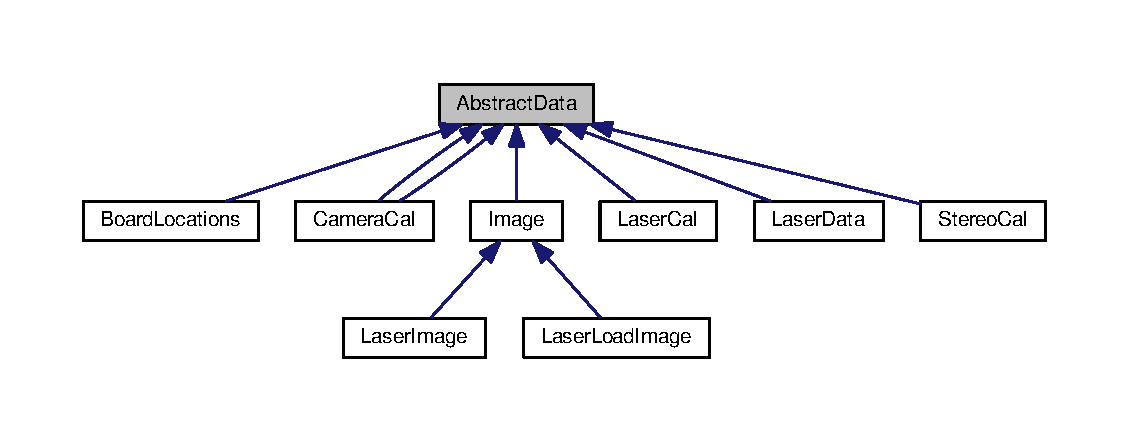
\includegraphics[width=350pt]{classAbstractData__inherit__graph}
\end{center}
\end{figure}
\subsection*{Public Member Functions}
\begin{DoxyCompactItemize}
\item 
virtual void \hyperlink{classAbstractData_ab43309236fd644fd303b4b1468a87d86}{read\+File} (std\+::string filename)
\begin{DoxyCompactList}\small\item\em abstract memeber to read data from a file using a filename \end{DoxyCompactList}\item 
virtual void \hyperlink{classAbstractData_a338dce47a9901032fd7b908a1c6df514}{write\+File} (std\+::string filename)
\begin{DoxyCompactList}\small\item\em abstract memeber to write data from a file using a filename \end{DoxyCompactList}\item 
virtual Q\+String\+List \hyperlink{classAbstractData_af9276f9e783765db82c8a7150c0ec632}{read\+D\+B\+Tables} ()
\begin{DoxyCompactList}\small\item\em abstract memeber to read data from a database \end{DoxyCompactList}\item 
virtual void \hyperlink{classAbstractData_a6eaaee3b3926d9044649249e7b665c66}{write\+DB} (std\+::string table)
\begin{DoxyCompactList}\small\item\em abstract memeber to write data to a database \end{DoxyCompactList}\item 
virtual std\+::string {\bfseries get\+D\+B\+Table\+Description} ()\hypertarget{classAbstractData_a09d6d5beb359c704c58d41d9710a167f}{}\label{classAbstractData_a09d6d5beb359c704c58d41d9710a167f}

\item 
virtual int \hyperlink{classAbstractData_a11dc7c98def9fb8b2c622d9af63cdd0e}{get\+Version} ()
\begin{DoxyCompactList}\small\item\em the version number of the datatype so that you can preserve backwards compatibility. \end{DoxyCompactList}\item 
virtual bool \hyperlink{classAbstractData_a8524756b3b36642ab007296da748b6db}{is\+Loaded} ()
\begin{DoxyCompactList}\small\item\em a simple check to determine if the data is loaded \end{DoxyCompactList}\end{DoxyCompactItemize}
\subsection*{Protected Attributes}
\begin{DoxyCompactItemize}
\item 
std\+::string \hyperlink{classAbstractData_a9e0d49b44dafbbb9db044d3b53dc7be2}{data\+Type}\hypertarget{classAbstractData_a9e0d49b44dafbbb9db044d3b53dc7be2}{}\label{classAbstractData_a9e0d49b44dafbbb9db044d3b53dc7be2}

\begin{DoxyCompactList}\small\item\em a brief description of what type of data this is. intended for use when reading human readble file formats like yaml, csv or xml. \end{DoxyCompactList}\item 
int \hyperlink{classAbstractData_a39401138096e4825fa782a7436efb3c8}{version}\hypertarget{classAbstractData_a39401138096e4825fa782a7436efb3c8}{}\label{classAbstractData_a39401138096e4825fa782a7436efb3c8}

\begin{DoxyCompactList}\small\item\em the version number see \hyperlink{classAbstractData_a11dc7c98def9fb8b2c622d9af63cdd0e}{Abstract\+Data\+::get\+Version()} \end{DoxyCompactList}\item 
bool \hyperlink{classAbstractData_a9c66c08ff8a48be7e194d30754e96dc0}{loaded}\hypertarget{classAbstractData_a9c66c08ff8a48be7e194d30754e96dc0}{}\label{classAbstractData_a9c66c08ff8a48be7e194d30754e96dc0}

\begin{DoxyCompactList}\small\item\em is the thing loaded see \hyperlink{classAbstractData_a8524756b3b36642ab007296da748b6db}{Abstract\+Data\+::is\+Loaded()} \end{DoxyCompactList}\end{DoxyCompactItemize}


\subsection{Member Function Documentation}
\index{Abstract\+Data@{Abstract\+Data}!get\+Version@{get\+Version}}
\index{get\+Version@{get\+Version}!Abstract\+Data@{Abstract\+Data}}
\subsubsection[{\texorpdfstring{get\+Version()}{getVersion()}}]{\setlength{\rightskip}{0pt plus 5cm}virtual int Abstract\+Data\+::get\+Version (
\begin{DoxyParamCaption}
{}
\end{DoxyParamCaption}
)\hspace{0.3cm}{\ttfamily [inline]}, {\ttfamily [virtual]}}\hypertarget{classAbstractData_a11dc7c98def9fb8b2c622d9af63cdd0e}{}\label{classAbstractData_a11dc7c98def9fb8b2c622d9af63cdd0e}


the version number of the datatype so that you can preserve backwards compatibility. 

\begin{DoxyReturn}{Returns}
the version number as an integer 
\end{DoxyReturn}
\index{Abstract\+Data@{Abstract\+Data}!is\+Loaded@{is\+Loaded}}
\index{is\+Loaded@{is\+Loaded}!Abstract\+Data@{Abstract\+Data}}
\subsubsection[{\texorpdfstring{is\+Loaded()}{isLoaded()}}]{\setlength{\rightskip}{0pt plus 5cm}virtual bool Abstract\+Data\+::is\+Loaded (
\begin{DoxyParamCaption}
{}
\end{DoxyParamCaption}
)\hspace{0.3cm}{\ttfamily [inline]}, {\ttfamily [virtual]}}\hypertarget{classAbstractData_a8524756b3b36642ab007296da748b6db}{}\label{classAbstractData_a8524756b3b36642ab007296da748b6db}


a simple check to determine if the data is loaded 

\begin{DoxyReturn}{Returns}
true if loaded otherwise false 
\end{DoxyReturn}


Reimplemented in \hyperlink{classImage_a7a3bf833c8e740d483f46eff90c90889}{Image}.

\index{Abstract\+Data@{Abstract\+Data}!read\+D\+B\+Tables@{read\+D\+B\+Tables}}
\index{read\+D\+B\+Tables@{read\+D\+B\+Tables}!Abstract\+Data@{Abstract\+Data}}
\subsubsection[{\texorpdfstring{read\+D\+B\+Tables()}{readDBTables()}}]{\setlength{\rightskip}{0pt plus 5cm}virtual Q\+String\+List Abstract\+Data\+::read\+D\+B\+Tables (
\begin{DoxyParamCaption}
{}
\end{DoxyParamCaption}
)\hspace{0.3cm}{\ttfamily [inline]}, {\ttfamily [virtual]}}\hypertarget{classAbstractData_af9276f9e783765db82c8a7150c0ec632}{}\label{classAbstractData_af9276f9e783765db82c8a7150c0ec632}


abstract memeber to read data from a database 


\begin{DoxyParams}{Parameters}
{\em table} & the table you want to write to \\
\hline
\end{DoxyParams}
\begin{DoxyNote}{Note}
unless overridden this function will just print an error to the screen 
\end{DoxyNote}
\index{Abstract\+Data@{Abstract\+Data}!read\+File@{read\+File}}
\index{read\+File@{read\+File}!Abstract\+Data@{Abstract\+Data}}
\subsubsection[{\texorpdfstring{read\+File(std\+::string filename)}{readFile(std::string filename)}}]{\setlength{\rightskip}{0pt plus 5cm}virtual void Abstract\+Data\+::read\+File (
\begin{DoxyParamCaption}
\item[{std\+::string}]{filename}
\end{DoxyParamCaption}
)\hspace{0.3cm}{\ttfamily [inline]}, {\ttfamily [virtual]}}\hypertarget{classAbstractData_ab43309236fd644fd303b4b1468a87d86}{}\label{classAbstractData_ab43309236fd644fd303b4b1468a87d86}


abstract memeber to read data from a file using a filename 


\begin{DoxyParams}{Parameters}
{\em filename} & the location of the file you wish to read from \\
\hline
\end{DoxyParams}
\begin{DoxyNote}{Note}
unless overridden this function will just print an error to the screen 
\end{DoxyNote}


Reimplemented in \hyperlink{classCameraCal_a2f47fc4ab16adcdd6269184340e087ed}{Camera\+Cal}, \hyperlink{classCameraCal_a2f47fc4ab16adcdd6269184340e087ed}{Camera\+Cal}, \hyperlink{classLaserData_ae7d37ab61d0ee00538c33740ac0ad7ab}{Laser\+Data}, \hyperlink{classStereoCal_a88808ab1dcc56daa4838bee7b4d1eadb}{Stereo\+Cal}, \hyperlink{classLaserCal_a8b046415d554ab9a0612a5f55f5e92ce}{Laser\+Cal}, and \hyperlink{classBoardLocations_aaf84c2db5212ae94ddece86c333befb8}{Board\+Locations}.

\index{Abstract\+Data@{Abstract\+Data}!write\+DB@{write\+DB}}
\index{write\+DB@{write\+DB}!Abstract\+Data@{Abstract\+Data}}
\subsubsection[{\texorpdfstring{write\+D\+B(std\+::string table)}{writeDB(std::string table)}}]{\setlength{\rightskip}{0pt plus 5cm}virtual void Abstract\+Data\+::write\+DB (
\begin{DoxyParamCaption}
\item[{std\+::string}]{table}
\end{DoxyParamCaption}
)\hspace{0.3cm}{\ttfamily [inline]}, {\ttfamily [virtual]}}\hypertarget{classAbstractData_a6eaaee3b3926d9044649249e7b665c66}{}\label{classAbstractData_a6eaaee3b3926d9044649249e7b665c66}


abstract memeber to write data to a database 


\begin{DoxyParams}{Parameters}
{\em table} & the table you want to read from \\
\hline
\end{DoxyParams}
\begin{DoxyNote}{Note}
unless overridden this function will just print an error to the screen 
\end{DoxyNote}
\index{Abstract\+Data@{Abstract\+Data}!write\+File@{write\+File}}
\index{write\+File@{write\+File}!Abstract\+Data@{Abstract\+Data}}
\subsubsection[{\texorpdfstring{write\+File(std\+::string filename)}{writeFile(std::string filename)}}]{\setlength{\rightskip}{0pt plus 5cm}virtual void Abstract\+Data\+::write\+File (
\begin{DoxyParamCaption}
\item[{std\+::string}]{filename}
\end{DoxyParamCaption}
)\hspace{0.3cm}{\ttfamily [inline]}, {\ttfamily [virtual]}}\hypertarget{classAbstractData_a338dce47a9901032fd7b908a1c6df514}{}\label{classAbstractData_a338dce47a9901032fd7b908a1c6df514}


abstract memeber to write data from a file using a filename 


\begin{DoxyParams}{Parameters}
{\em filename} & the location of the file you wish to write to \\
\hline
\end{DoxyParams}
\begin{DoxyNote}{Note}
unless overridden this function will just print an error to the screen 
\end{DoxyNote}


Reimplemented in \hyperlink{classCameraCal_aed026a2f07ceffeaf5591072cae13f99}{Camera\+Cal}, \hyperlink{classCameraCal_aed026a2f07ceffeaf5591072cae13f99}{Camera\+Cal}, \hyperlink{classLaserData_abef00b09c8ee06285c0683198de5a9e3}{Laser\+Data}, \hyperlink{classStereoCal_ac31d3a00ccfb336f0755a12053609710}{Stereo\+Cal}, \hyperlink{classLaserCal_a08ba4fb6840a73989f75d2ec4aea3fcd}{Laser\+Cal}, and \hyperlink{classBoardLocations_a9355491bd25943d2ad4f725fc8aae849}{Board\+Locations}.



The documentation for this class was generated from the following files\+:\begin{DoxyCompactItemize}
\item 
/home/labrat/\+Desktop/cam-\/proc/src/lib\+Cam/include/abstractdata.\+h\item 
/home/labrat/\+Desktop/cam-\/proc/src/lib\+Cam/include/abstractdata.\+cpp\end{DoxyCompactItemize}

\hypertarget{classAbstractToolbar}{}\section{Abstract\+Toolbar Class Reference}
\label{classAbstractToolbar}\index{Abstract\+Toolbar@{Abstract\+Toolbar}}


Inheritance diagram for Abstract\+Toolbar\+:\nopagebreak
\begin{figure}[H]
\begin{center}
\leavevmode
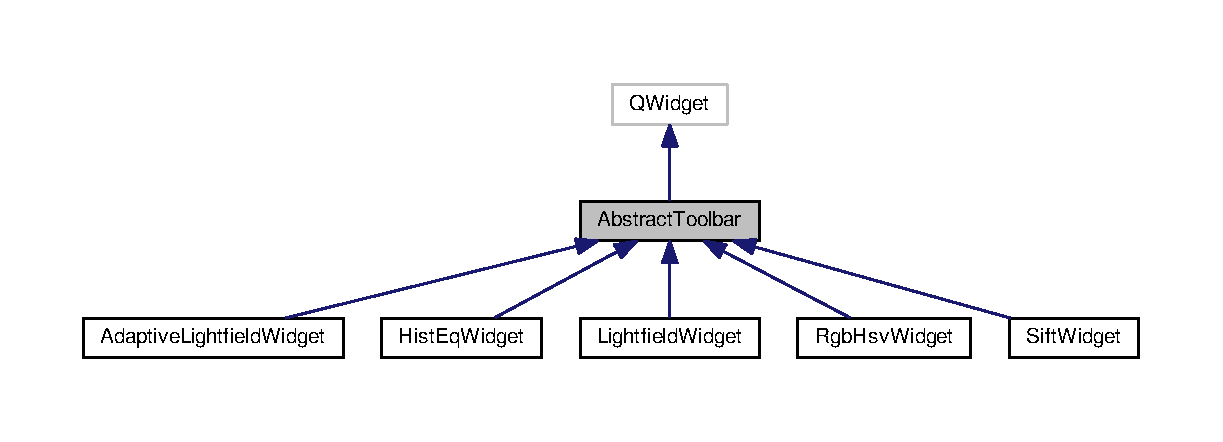
\includegraphics[width=350pt]{classAbstractToolbar__inherit__graph}
\end{center}
\end{figure}


Collaboration diagram for Abstract\+Toolbar\+:\nopagebreak
\begin{figure}[H]
\begin{center}
\leavevmode
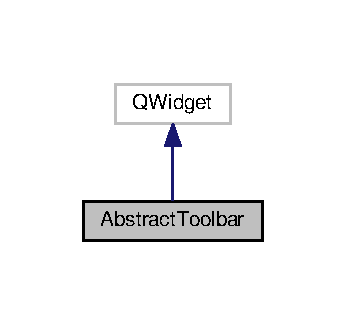
\includegraphics[width=166pt]{classAbstractToolbar__coll__graph}
\end{center}
\end{figure}
\subsection*{Public Member Functions}
\begin{DoxyCompactItemize}
\item 
{\bfseries Abstract\+Toolbar} (Q\+Widget $\ast$parent=0)\hypertarget{classAbstractToolbar_a9f7e3ff248be380c39f3370f585d356d}{}\label{classAbstractToolbar_a9f7e3ff248be380c39f3370f585d356d}

\item 
virtual \hyperlink{classImageProcessor}{Image\+Processor} \& {\bfseries get\+Processor} ()=0\hypertarget{classAbstractToolbar_adb5af62a3c4a558c69101bdd6f3d1dc1}{}\label{classAbstractToolbar_adb5af62a3c4a558c69101bdd6f3d1dc1}

\item 
virtual void {\bfseries update} ()=0\hypertarget{classAbstractToolbar_aac72f6530afd606e8f9d272f8459ef43}{}\label{classAbstractToolbar_aac72f6530afd606e8f9d272f8459ef43}

\item 
virtual std\+::string {\bfseries get\+Name} ()\hypertarget{classAbstractToolbar_ab367628bff78aa9fe6b31c2cf09c41d6}{}\label{classAbstractToolbar_ab367628bff78aa9fe6b31c2cf09c41d6}

\end{DoxyCompactItemize}


The documentation for this class was generated from the following files\+:\begin{DoxyCompactItemize}
\item 
/home/labrat/\+Desktop/cam-\/proc/src/lib\+Cam/qtinclude/abstracttoolbar.\+h\item 
/home/labrat/\+Desktop/cam-\/proc/src/lib\+Cam/qtinclude/abstracttoolbar.\+cpp\end{DoxyCompactItemize}

\hypertarget{classAdaptiveLightfield}{}\section{Adaptive\+Lightfield Class Reference}
\label{classAdaptiveLightfield}\index{Adaptive\+Lightfield@{Adaptive\+Lightfield}}


Inheritance diagram for Adaptive\+Lightfield\+:\nopagebreak
\begin{figure}[H]
\begin{center}
\leavevmode
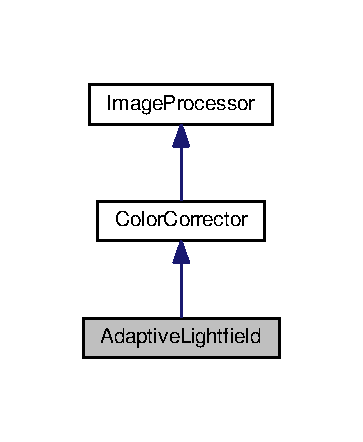
\includegraphics[width=174pt]{classAdaptiveLightfield__inherit__graph}
\end{center}
\end{figure}


Collaboration diagram for Adaptive\+Lightfield\+:\nopagebreak
\begin{figure}[H]
\begin{center}
\leavevmode
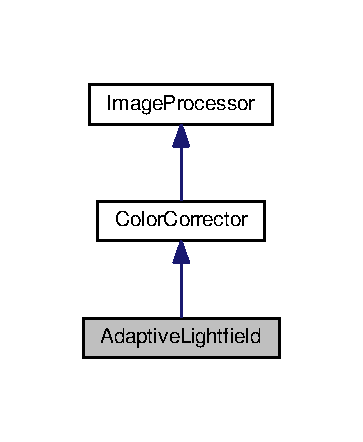
\includegraphics[width=174pt]{classAdaptiveLightfield__coll__graph}
\end{center}
\end{figure}
\subsection*{Public Member Functions}
\begin{DoxyCompactItemize}
\item 
void {\bfseries forward\+Directory} ()\hypertarget{classAdaptiveLightfield_a193b5267bd93c58fc303dfd8dd713c71}{}\label{classAdaptiveLightfield_a193b5267bd93c58fc303dfd8dd713c71}

\item 
\hyperlink{classImage}{Image} {\bfseries adaptive\+Background\+L\+F\+Corrector} (int ind)\hypertarget{classAdaptiveLightfield_af114596f625e67260c93e1ecdca42e07}{}\label{classAdaptiveLightfield_af114596f625e67260c93e1ecdca42e07}

\item 
void {\bfseries static\+Background\+L\+F\+Corrector} ()\hypertarget{classAdaptiveLightfield_ad824c77f245a5257ef9d63f1245790c2}{}\label{classAdaptiveLightfield_ad824c77f245a5257ef9d63f1245790c2}

\item 
void {\bfseries sliding\+Background\+L\+F\+Corrector} ()\hypertarget{classAdaptiveLightfield_a57da703b77df5798a858df348f8b9d11}{}\label{classAdaptiveLightfield_a57da703b77df5798a858df348f8b9d11}

\item 
void {\bfseries fixed\+Slide\+Background\+L\+F\+Corrector} ()\hypertarget{classAdaptiveLightfield_a4adca7182ab1c7bc9edb11998fe474b9}{}\label{classAdaptiveLightfield_a4adca7182ab1c7bc9edb11998fe474b9}

\item 
void {\bfseries set\+ContrastA} (float in)\hypertarget{classAdaptiveLightfield_a4c254a9f404bf7570189c8f88d0e03e9}{}\label{classAdaptiveLightfield_a4c254a9f404bf7570189c8f88d0e03e9}

\item 
void {\bfseries set\+BrightnessA} (float in)\hypertarget{classAdaptiveLightfield_a016cc9d5a5426053c7ad3f1ca6dea3a0}{}\label{classAdaptiveLightfield_a016cc9d5a5426053c7ad3f1ca6dea3a0}

\item 
void {\bfseries set\+ContrastB} (float in)\hypertarget{classAdaptiveLightfield_af82d6fd4ace796e51a504aa4b08865c4}{}\label{classAdaptiveLightfield_af82d6fd4ace796e51a504aa4b08865c4}

\item 
void {\bfseries set\+BrightnessB} (float in)\hypertarget{classAdaptiveLightfield_aed74c18f2288a64236be497b42439df2}{}\label{classAdaptiveLightfield_aed74c18f2288a64236be497b42439df2}

\item 
void {\bfseries set\+Method} (L\+F\+Method in)\hypertarget{classAdaptiveLightfield_ae3c1a7140b6830b65fc56170a9b3953d}{}\label{classAdaptiveLightfield_ae3c1a7140b6830b65fc56170a9b3953d}

\item 
void {\bfseries set\+Mat\+Type} (int type)\hypertarget{classAdaptiveLightfield_a87ad5c9596afd7bf3d106fb332da926d}{}\label{classAdaptiveLightfield_a87ad5c9596afd7bf3d106fb332da926d}

\item 
void {\bfseries set\+Mat\+Out\+Type} (int type)\hypertarget{classAdaptiveLightfield_a2bc5c9ce2b52491a3954c767f89a4a24}{}\label{classAdaptiveLightfield_a2bc5c9ce2b52491a3954c767f89a4a24}

\item 
void {\bfseries set\+Blur\+Size} (int sz)\hypertarget{classAdaptiveLightfield_a741ac73e468db5fc8448fbdeadc1771d}{}\label{classAdaptiveLightfield_a741ac73e468db5fc8448fbdeadc1771d}

\item 
void {\bfseries set\+Cut\+Off\+SD} (double thresh)\hypertarget{classAdaptiveLightfield_a829937f1ff19df1bce0a8fb6e5815634}{}\label{classAdaptiveLightfield_a829937f1ff19df1bce0a8fb6e5815634}

\item 
void {\bfseries set\+Win\+Max} (double sz)\hypertarget{classAdaptiveLightfield_abaf686947c3ab45ce1845ec547d2d0fc}{}\label{classAdaptiveLightfield_abaf686947c3ab45ce1845ec547d2d0fc}

\item 
void {\bfseries log\+Run\+Params} (std\+::string fun)\hypertarget{classAdaptiveLightfield_a267f68acd001ce529cd55826fa0e048f}{}\label{classAdaptiveLightfield_a267f68acd001ce529cd55826fa0e048f}

\item 
void {\bfseries log\+Im\+Run\+Params} (std\+::string fun)\hypertarget{classAdaptiveLightfield_a451e1001a4490b48f6d6987bf1880e79}{}\label{classAdaptiveLightfield_a451e1001a4490b48f6d6987bf1880e79}

\item 
void {\bfseries log\+Im\+Stats} (std\+::string out)\hypertarget{classAdaptiveLightfield_a913705c26085937b00f40f7e9d54d03f}{}\label{classAdaptiveLightfield_a913705c26085937b00f40f7e9d54d03f}

\item 
virtual void {\bfseries save} ()\hypertarget{classAdaptiveLightfield_a098c869cd368f893cd08c228d28f58dd}{}\label{classAdaptiveLightfield_a098c869cd368f893cd08c228d28f58dd}

\end{DoxyCompactItemize}
\subsection*{Protected Member Functions}
\begin{DoxyCompactItemize}
\item 
void {\bfseries run\+Operations} ()\hypertarget{classAdaptiveLightfield_a5b060298ae68862e6f125a0c390ec229}{}\label{classAdaptiveLightfield_a5b060298ae68862e6f125a0c390ec229}

\end{DoxyCompactItemize}
\subsection*{Additional Inherited Members}


The documentation for this class was generated from the following files\+:\begin{DoxyCompactItemize}
\item 
/home/labrat/\+Desktop/cam-\/proc/src/color\+Corrector/src/adaptivelightfield.\+h\item 
/home/labrat/\+Desktop/cam-\/proc/src/color\+Corrector/src/adaptivelightfield.\+cpp\end{DoxyCompactItemize}

\hypertarget{classAdaptiveLightfieldWidget}{}\section{Adaptive\+Lightfield\+Widget Class Reference}
\label{classAdaptiveLightfieldWidget}\index{Adaptive\+Lightfield\+Widget@{Adaptive\+Lightfield\+Widget}}


Inheritance diagram for Adaptive\+Lightfield\+Widget\+:\nopagebreak
\begin{figure}[H]
\begin{center}
\leavevmode
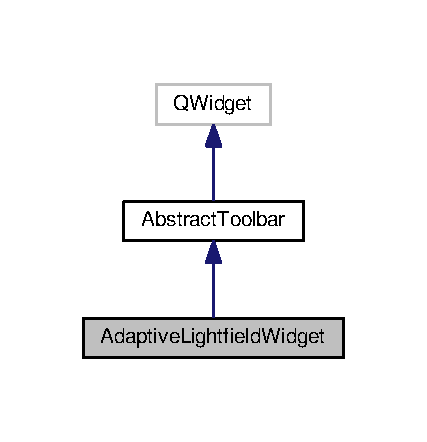
\includegraphics[width=205pt]{classAdaptiveLightfieldWidget__inherit__graph}
\end{center}
\end{figure}


Collaboration diagram for Adaptive\+Lightfield\+Widget\+:\nopagebreak
\begin{figure}[H]
\begin{center}
\leavevmode
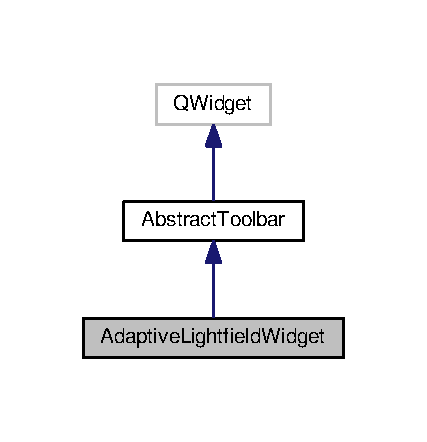
\includegraphics[width=205pt]{classAdaptiveLightfieldWidget__coll__graph}
\end{center}
\end{figure}
\subsection*{Public Member Functions}
\begin{DoxyCompactItemize}
\item 
{\bfseries Adaptive\+Lightfield\+Widget} (\hyperlink{classAbstractToolbar}{Abstract\+Toolbar} $\ast$parent=0)\hypertarget{classAdaptiveLightfieldWidget_ad32d99f265f24e082ad7f9a2d7bc50f9}{}\label{classAdaptiveLightfieldWidget_ad32d99f265f24e082ad7f9a2d7bc50f9}

\item 
void \hyperlink{classAdaptiveLightfieldWidget_ac1b36b7d01656ae440c7b4b7788fcf1a}{update} ()
\item 
\hyperlink{classAdaptiveLightfield}{Adaptive\+Lightfield} \& {\bfseries get\+Processor} ()\hypertarget{classAdaptiveLightfieldWidget_a1cd5d33f54de0a6bdd1dbca05c5c981e}{}\label{classAdaptiveLightfieldWidget_a1cd5d33f54de0a6bdd1dbca05c5c981e}

\item 
std\+::string {\bfseries get\+Name} ()\hypertarget{classAdaptiveLightfieldWidget_a820335b94b940e1d52a5ca1745d996b0}{}\label{classAdaptiveLightfieldWidget_a820335b94b940e1d52a5ca1745d996b0}

\end{DoxyCompactItemize}


\subsection{Member Function Documentation}
\index{Adaptive\+Lightfield\+Widget@{Adaptive\+Lightfield\+Widget}!update@{update}}
\index{update@{update}!Adaptive\+Lightfield\+Widget@{Adaptive\+Lightfield\+Widget}}
\subsubsection[{\texorpdfstring{update()}{update()}}]{\setlength{\rightskip}{0pt plus 5cm}void Adaptive\+Lightfield\+Widget\+::update (
\begin{DoxyParamCaption}
{}
\end{DoxyParamCaption}
)\hspace{0.3cm}{\ttfamily [virtual]}}\hypertarget{classAdaptiveLightfieldWidget_ac1b36b7d01656ae440c7b4b7788fcf1a}{}\label{classAdaptiveLightfieldWidget_ac1b36b7d01656ae440c7b4b7788fcf1a}
we need to override the \hyperlink{classAbstractToolbar}{Abstract\+Toolbar} stuff 

Implements \hyperlink{classAbstractToolbar}{Abstract\+Toolbar}.



The documentation for this class was generated from the following files\+:\begin{DoxyCompactItemize}
\item 
/home/labrat/\+Desktop/cam-\/proc/src/color\+Corrector/ui/adaptivelightfieldwidget.\+h\item 
/home/labrat/\+Desktop/cam-\/proc/src/color\+Corrector/ui/adaptivelightfieldwidget.\+cpp\end{DoxyCompactItemize}

\hypertarget{classaddDialogXmlExcelCsv}{}\section{add\+Dialog\+Xml\+Excel\+Csv Class Reference}
\label{classaddDialogXmlExcelCsv}\index{add\+Dialog\+Xml\+Excel\+Csv@{add\+Dialog\+Xml\+Excel\+Csv}}


Inheritance diagram for add\+Dialog\+Xml\+Excel\+Csv\+:\nopagebreak
\begin{figure}[H]
\begin{center}
\leavevmode
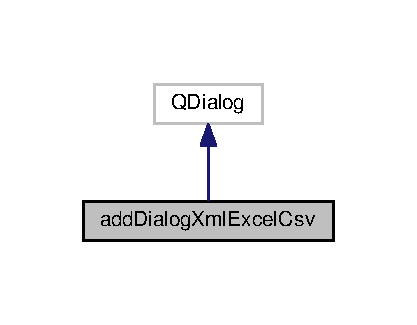
\includegraphics[width=200pt]{classaddDialogXmlExcelCsv__inherit__graph}
\end{center}
\end{figure}


Collaboration diagram for add\+Dialog\+Xml\+Excel\+Csv\+:\nopagebreak
\begin{figure}[H]
\begin{center}
\leavevmode
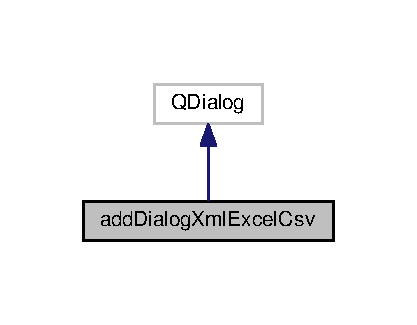
\includegraphics[width=200pt]{classaddDialogXmlExcelCsv__coll__graph}
\end{center}
\end{figure}
\subsection*{Public Member Functions}
\begin{DoxyCompactItemize}
\item 
{\bfseries add\+Dialog\+Xml\+Excel\+Csv} (Q\+Widget $\ast$parent=nullptr)\hypertarget{classaddDialogXmlExcelCsv_a47b3e548f9b75e2b1a7ba0ce38728d34}{}\label{classaddDialogXmlExcelCsv_a47b3e548f9b75e2b1a7ba0ce38728d34}

\item 
\hyperlink{classinsertValuesXmlExcelCsv}{insert\+Values\+Xml\+Excel\+Csv} {\bfseries getinsert\+Values\+Xml\+Excel\+Csv} () const \hypertarget{classaddDialogXmlExcelCsv_a2e04de20e93fe34c65430aab248b9614}{}\label{classaddDialogXmlExcelCsv_a2e04de20e93fe34c65430aab248b9614}

\item 
void {\bfseries set\+Model} (Q\+Abstract\+Item\+Model $\ast$model)\hypertarget{classaddDialogXmlExcelCsv_a179cd39836d5eb09a6c52a65490f8184}{}\label{classaddDialogXmlExcelCsv_a179cd39836d5eb09a6c52a65490f8184}

\end{DoxyCompactItemize}


The documentation for this class was generated from the following files\+:\begin{DoxyCompactItemize}
\item 
/home/labrat/\+Desktop/cam-\/proc/src/\+E\+R\+Database\+System/ui/adddialogxmlexcelcsv.\+h\item 
/home/labrat/\+Desktop/cam-\/proc/src/\+E\+R\+Database\+System/ui/adddialogxmlexcelcsv.\+cpp\end{DoxyCompactItemize}

\hypertarget{classaddItemFirstNestedTableDialog}{}\section{add\+Item\+First\+Nested\+Table\+Dialog Class Reference}
\label{classaddItemFirstNestedTableDialog}\index{add\+Item\+First\+Nested\+Table\+Dialog@{add\+Item\+First\+Nested\+Table\+Dialog}}


Inheritance diagram for add\+Item\+First\+Nested\+Table\+Dialog\+:\nopagebreak
\begin{figure}[H]
\begin{center}
\leavevmode
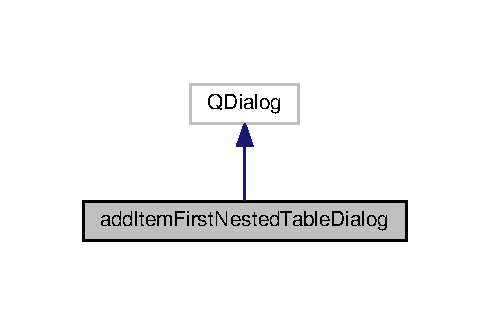
\includegraphics[width=235pt]{classaddItemFirstNestedTableDialog__inherit__graph}
\end{center}
\end{figure}


Collaboration diagram for add\+Item\+First\+Nested\+Table\+Dialog\+:\nopagebreak
\begin{figure}[H]
\begin{center}
\leavevmode
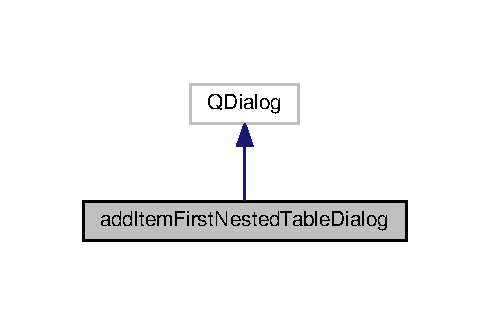
\includegraphics[width=235pt]{classaddItemFirstNestedTableDialog__coll__graph}
\end{center}
\end{figure}
\subsection*{Public Member Functions}
\begin{DoxyCompactItemize}
\item 
{\bfseries add\+Item\+First\+Nested\+Table\+Dialog} (Q\+Widget $\ast$parent=nullptr)\hypertarget{classaddItemFirstNestedTableDialog_a0562a4a6147c4b8db2cd1208399dbe35}{}\label{classaddItemFirstNestedTableDialog_a0562a4a6147c4b8db2cd1208399dbe35}

\item 
\hyperlink{classitem}{item} {\bfseries items} () const \hypertarget{classaddItemFirstNestedTableDialog_acb196230bb4ee8d22d19049d4ad66480}{}\label{classaddItemFirstNestedTableDialog_acb196230bb4ee8d22d19049d4ad66480}

\end{DoxyCompactItemize}


The documentation for this class was generated from the following files\+:\begin{DoxyCompactItemize}
\item 
/home/labrat/\+Desktop/cam-\/proc/src/\+E\+R\+Database\+System/ui/additemfirstnestedtabledialog.\+h\item 
/home/labrat/\+Desktop/cam-\/proc/src/\+E\+R\+Database\+System/ui/additemfirstnestedtabledialog.\+cpp\end{DoxyCompactItemize}

\hypertarget{classaddRoiDialog}{}\section{add\+Roi\+Dialog Class Reference}
\label{classaddRoiDialog}\index{add\+Roi\+Dialog@{add\+Roi\+Dialog}}


Inheritance diagram for add\+Roi\+Dialog\+:\nopagebreak
\begin{figure}[H]
\begin{center}
\leavevmode
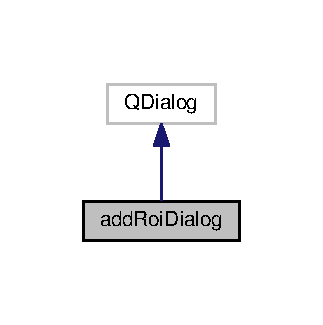
\includegraphics[width=155pt]{classaddRoiDialog__inherit__graph}
\end{center}
\end{figure}


Collaboration diagram for add\+Roi\+Dialog\+:\nopagebreak
\begin{figure}[H]
\begin{center}
\leavevmode
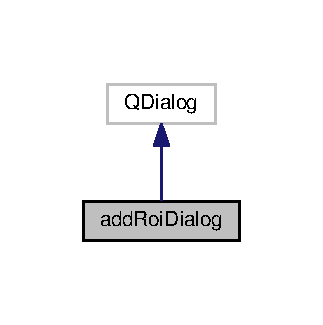
\includegraphics[width=155pt]{classaddRoiDialog__coll__graph}
\end{center}
\end{figure}
\subsection*{Public Member Functions}
\begin{DoxyCompactItemize}
\item 
{\bfseries add\+Roi\+Dialog} (Q\+Widget $\ast$parent=nullptr)\hypertarget{classaddRoiDialog_a8b7fc43685d1f03fdc1b46aa89747649}{}\label{classaddRoiDialog_a8b7fc43685d1f03fdc1b46aa89747649}

\item 
\hyperlink{classitemRoi}{item\+Roi} $\ast$ {\bfseries item} () const \hypertarget{classaddRoiDialog_a7317773bb81dbb977cc218bcde3ea818}{}\label{classaddRoiDialog_a7317773bb81dbb977cc218bcde3ea818}

\end{DoxyCompactItemize}


The documentation for this class was generated from the following files\+:\begin{DoxyCompactItemize}
\item 
/home/labrat/\+Desktop/cam-\/proc/src/\+E\+R\+Database\+System/ui/addroidialog.\+h\item 
/home/labrat/\+Desktop/cam-\/proc/src/\+E\+R\+Database\+System/ui/addroidialog.\+cpp\end{DoxyCompactItemize}

\hypertarget{classautoSizeBoard}{}\section{auto\+Size\+Board Class Reference}
\label{classautoSizeBoard}\index{auto\+Size\+Board@{auto\+Size\+Board}}
\subsection*{Public Member Functions}
\begin{DoxyCompactItemize}
\item 
void {\bfseries setup\+Chessboard} (int num\+Horizontal, int num\+Vertical, float cell\+Dim)\hypertarget{classautoSizeBoard_a78d5effbeb345ab558e3005bc647ea75}{}\label{classautoSizeBoard_a78d5effbeb345ab558e3005bc647ea75}

\item 
bool {\bfseries find\+Chessboard\+Corners} (Mat image, int flags)\hypertarget{classautoSizeBoard_a708bc58bb6378d1e68bdcd88f7fb6ce0}{}\label{classautoSizeBoard_a708bc58bb6378d1e68bdcd88f7fb6ce0}

\item 
int {\bfseries get\+Num\+Detected\+Squares} ()\hypertarget{classautoSizeBoard_a42ace17d6b62d29f479ba825c6ecfa13}{}\label{classautoSizeBoard_a42ace17d6b62d29f479ba825c6ecfa13}

\item 
Size {\bfseries get\+Detected\+Size} ()\hypertarget{classautoSizeBoard_aeb0f981b974051e6cdc4144483916163}{}\label{classautoSizeBoard_aeb0f981b974051e6cdc4144483916163}

\item 
Size {\bfseries get\+Physical\+Size} ()\hypertarget{classautoSizeBoard_ad8176f03e68c47c0cfe2113d3d8fdf12}{}\label{classautoSizeBoard_ad8176f03e68c47c0cfe2113d3d8fdf12}

\item 
int {\bfseries get\+Detected\+Rows} ()\hypertarget{classautoSizeBoard_a3b83e798ed4ebeefc17fb75268e5aa8a}{}\label{classautoSizeBoard_a3b83e798ed4ebeefc17fb75268e5aa8a}

\item 
int {\bfseries get\+Detected\+Cols} ()\hypertarget{classautoSizeBoard_a031e73274170e488ef06e6529d376f2b}{}\label{classautoSizeBoard_a031e73274170e488ef06e6529d376f2b}

\item 
vector$<$ Point2f $>$ {\bfseries get\+Detected\+Corners} ()\hypertarget{classautoSizeBoard_a092dfb83b61b64ad0c074c96335d8032}{}\label{classautoSizeBoard_a092dfb83b61b64ad0c074c96335d8032}

\item 
vector$<$ Point3f $>$ {\bfseries get\+Obj} ()\hypertarget{classautoSizeBoard_a89915a169a019d0e542386d81dbc2e66}{}\label{classautoSizeBoard_a89915a169a019d0e542386d81dbc2e66}

\item 
void {\bfseries set\+Min\+Board} (int row, int col)\hypertarget{classautoSizeBoard_aabf153bce08fd66c74c373d6641fd18e}{}\label{classautoSizeBoard_aabf153bce08fd66c74c373d6641fd18e}

\item 
float {\bfseries get\+Cell\+Size} ()\hypertarget{classautoSizeBoard_aab2271090efcd2fdbc2c4a7bfcd83865}{}\label{classautoSizeBoard_aab2271090efcd2fdbc2c4a7bfcd83865}

\item 
void {\bfseries setup\+Chessboard} (int num\+Horizontal, int num\+Vertical, float cell\+Dim)\hypertarget{classautoSizeBoard_a78d5effbeb345ab558e3005bc647ea75}{}\label{classautoSizeBoard_a78d5effbeb345ab558e3005bc647ea75}

\item 
bool {\bfseries find\+Chessboard\+Corners} (Mat image, int flags)\hypertarget{classautoSizeBoard_a708bc58bb6378d1e68bdcd88f7fb6ce0}{}\label{classautoSizeBoard_a708bc58bb6378d1e68bdcd88f7fb6ce0}

\item 
int {\bfseries get\+Num\+Detected\+Squares} ()\hypertarget{classautoSizeBoard_a42ace17d6b62d29f479ba825c6ecfa13}{}\label{classautoSizeBoard_a42ace17d6b62d29f479ba825c6ecfa13}

\item 
Size {\bfseries get\+Detected\+Size} ()\hypertarget{classautoSizeBoard_aeb0f981b974051e6cdc4144483916163}{}\label{classautoSizeBoard_aeb0f981b974051e6cdc4144483916163}

\item 
Size {\bfseries get\+Physical\+Size} ()\hypertarget{classautoSizeBoard_ad8176f03e68c47c0cfe2113d3d8fdf12}{}\label{classautoSizeBoard_ad8176f03e68c47c0cfe2113d3d8fdf12}

\item 
int {\bfseries get\+Detected\+Rows} ()\hypertarget{classautoSizeBoard_a3b83e798ed4ebeefc17fb75268e5aa8a}{}\label{classautoSizeBoard_a3b83e798ed4ebeefc17fb75268e5aa8a}

\item 
int {\bfseries get\+Detected\+Cols} ()\hypertarget{classautoSizeBoard_a031e73274170e488ef06e6529d376f2b}{}\label{classautoSizeBoard_a031e73274170e488ef06e6529d376f2b}

\item 
vector$<$ Point2f $>$ {\bfseries get\+Detected\+Corners} ()\hypertarget{classautoSizeBoard_ab12d594e334279331ef0e2fd7e99f8d8}{}\label{classautoSizeBoard_ab12d594e334279331ef0e2fd7e99f8d8}

\item 
vector$<$ Point3f $>$ {\bfseries get\+Obj} ()\hypertarget{classautoSizeBoard_a11b95ae883d8ddb99c63c66ed52cf60d}{}\label{classautoSizeBoard_a11b95ae883d8ddb99c63c66ed52cf60d}

\item 
void {\bfseries set\+Min\+Board} (int row, int col)\hypertarget{classautoSizeBoard_aabf153bce08fd66c74c373d6641fd18e}{}\label{classautoSizeBoard_aabf153bce08fd66c74c373d6641fd18e}

\item 
float {\bfseries get\+Cell\+Size} ()\hypertarget{classautoSizeBoard_aab2271090efcd2fdbc2c4a7bfcd83865}{}\label{classautoSizeBoard_aab2271090efcd2fdbc2c4a7bfcd83865}

\end{DoxyCompactItemize}
\subsection*{Public Attributes}
\begin{DoxyCompactItemize}
\item 
float {\bfseries progress}\hypertarget{classautoSizeBoard_a332ce853a9edac61639b8c2af34b6f7a}{}\label{classautoSizeBoard_a332ce853a9edac61639b8c2af34b6f7a}

\end{DoxyCompactItemize}
\subsection*{Protected Member Functions}
\begin{DoxyCompactItemize}
\item 
void {\bfseries generate\+Obj} ()\hypertarget{classautoSizeBoard_affac18fa6bb8553f401ccfd423c03fb0}{}\label{classautoSizeBoard_affac18fa6bb8553f401ccfd423c03fb0}

\item 
void {\bfseries generate\+Obj} ()\hypertarget{classautoSizeBoard_affac18fa6bb8553f401ccfd423c03fb0}{}\label{classautoSizeBoard_affac18fa6bb8553f401ccfd423c03fb0}

\end{DoxyCompactItemize}
\subsection*{Protected Attributes}
\begin{DoxyCompactItemize}
\item 
int {\bfseries physical\+Rows}\hypertarget{classautoSizeBoard_aae58c0a1f5e9ae76c9a31c04524ace57}{}\label{classautoSizeBoard_aae58c0a1f5e9ae76c9a31c04524ace57}

\item 
int {\bfseries physical\+Cols}\hypertarget{classautoSizeBoard_a1884b5cc7001ec76631501fa0737065f}{}\label{classautoSizeBoard_a1884b5cc7001ec76631501fa0737065f}

\item 
int {\bfseries min\+Row}\hypertarget{classautoSizeBoard_a6b3dd38b48698d625f642b12db43f56f}{}\label{classautoSizeBoard_a6b3dd38b48698d625f642b12db43f56f}

\item 
int {\bfseries min\+Col}\hypertarget{classautoSizeBoard_a217efd12c653eee72b9b013f13fc4ecd}{}\label{classautoSizeBoard_a217efd12c653eee72b9b013f13fc4ecd}

\item 
float {\bfseries cell\+Size}\hypertarget{classautoSizeBoard_ae0cd7700bd982b2d10e96bf3c7b4ee83}{}\label{classautoSizeBoard_ae0cd7700bd982b2d10e96bf3c7b4ee83}

\item 
int {\bfseries detected\+Cols}\hypertarget{classautoSizeBoard_aec5026e68f143093084d82fd3ddcbee5}{}\label{classautoSizeBoard_aec5026e68f143093084d82fd3ddcbee5}

\item 
int {\bfseries detected\+Rows}\hypertarget{classautoSizeBoard_a11d4099e4d545253ceaeb9562cd71432}{}\label{classautoSizeBoard_a11d4099e4d545253ceaeb9562cd71432}

\item 
vector$<$ Point3f $>$ {\bfseries obj}\hypertarget{classautoSizeBoard_a5f78ee36b8452d0e5a8467c091107c6d}{}\label{classautoSizeBoard_a5f78ee36b8452d0e5a8467c091107c6d}

\item 
vector$<$ Point2f $>$ {\bfseries detected\+Corners}\hypertarget{classautoSizeBoard_a53c3230fb22912aa96eeef9fd0382ab5}{}\label{classautoSizeBoard_a53c3230fb22912aa96eeef9fd0382ab5}

\end{DoxyCompactItemize}


The documentation for this class was generated from the following files\+:\begin{DoxyCompactItemize}
\item 
/home/labrat/\+Desktop/cam-\/proc/src/camera\+Cal2/src/autosizeboard.\+h\item 
/home/labrat/\+Desktop/cam-\/proc/src/camera\+Cal2/src/autosizeboard.\+cpp\end{DoxyCompactItemize}

\hypertarget{classBioDatabaseUI}{}\section{Bio\+Database\+UI Class Reference}
\label{classBioDatabaseUI}\index{Bio\+Database\+UI@{Bio\+Database\+UI}}


Inheritance diagram for Bio\+Database\+UI\+:\nopagebreak
\begin{figure}[H]
\begin{center}
\leavevmode
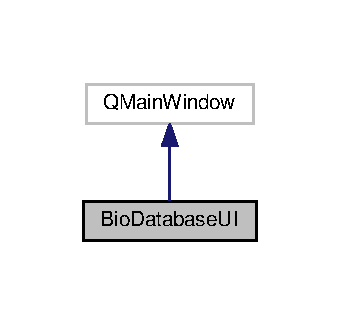
\includegraphics[width=163pt]{classBioDatabaseUI__inherit__graph}
\end{center}
\end{figure}


Collaboration diagram for Bio\+Database\+UI\+:\nopagebreak
\begin{figure}[H]
\begin{center}
\leavevmode
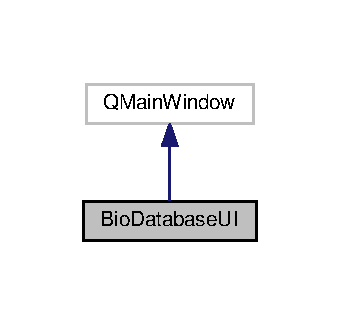
\includegraphics[width=163pt]{classBioDatabaseUI__coll__graph}
\end{center}
\end{figure}
\subsection*{Public Member Functions}
\begin{DoxyCompactItemize}
\item 
{\bfseries Bio\+Database\+UI} (Q\+Widget $\ast$parent=0)\hypertarget{classBioDatabaseUI_aec4e8a22e05dc5467acbec786ed384e5}{}\label{classBioDatabaseUI_aec4e8a22e05dc5467acbec786ed384e5}

\end{DoxyCompactItemize}


The documentation for this class was generated from the following files\+:\begin{DoxyCompactItemize}
\item 
/home/labrat/\+Desktop/cam-\/proc/src/bio\+Database/ui/biodatabaseui.\+h\item 
/home/labrat/\+Desktop/cam-\/proc/src/bio\+Database/ui/biodatabaseui.\+cpp\end{DoxyCompactItemize}

\hypertarget{classBoardLocations}{}\section{Board\+Locations Class Reference}
\label{classBoardLocations}\index{Board\+Locations@{Board\+Locations}}


Inheritance diagram for Board\+Locations\+:\nopagebreak
\begin{figure}[H]
\begin{center}
\leavevmode
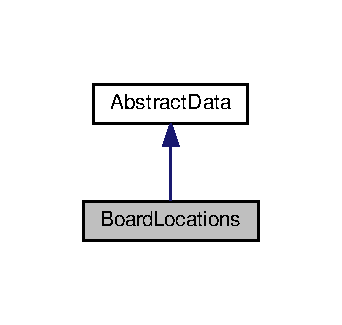
\includegraphics[width=164pt]{classBoardLocations__inherit__graph}
\end{center}
\end{figure}


Collaboration diagram for Board\+Locations\+:\nopagebreak
\begin{figure}[H]
\begin{center}
\leavevmode
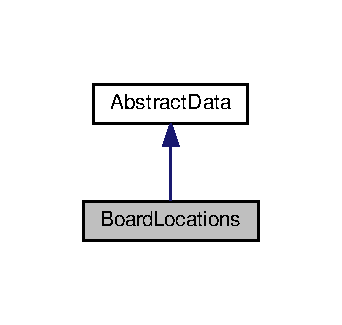
\includegraphics[width=164pt]{classBoardLocations__coll__graph}
\end{center}
\end{figure}
\subsection*{Public Member Functions}
\begin{DoxyCompactItemize}
\item 
void \hyperlink{classBoardLocations_aaf84c2db5212ae94ddece86c333befb8}{read\+File} (std\+::string filename)
\begin{DoxyCompactList}\small\item\em abstract memeber to read data from a file using a filename \end{DoxyCompactList}\item 
void \hyperlink{classBoardLocations_a9355491bd25943d2ad4f725fc8aae849}{write\+File} (std\+::string filename)
\begin{DoxyCompactList}\small\item\em abstract memeber to write data from a file using a filename \end{DoxyCompactList}\end{DoxyCompactItemize}
\subsection*{Public Attributes}
\begin{DoxyCompactItemize}
\item 
std\+::vector$<$ cv\+::\+Point2f $>$ {\bfseries get\+Board\+Points}\hypertarget{classBoardLocations_a66ae9db9985e92ab8466f96a46e96afb}{}\label{classBoardLocations_a66ae9db9985e92ab8466f96a46e96afb}

\item 
std\+::vector$<$ std\+::string $>$ {\bfseries filenames}\hypertarget{classBoardLocations_a7a970e1854031f1265817a7a471eca6b}{}\label{classBoardLocations_a7a970e1854031f1265817a7a471eca6b}

\item 
std\+::vector$<$ cv\+::\+Mat $>$ {\bfseries translation\+Vectors}\hypertarget{classBoardLocations_a7f9e70f9b8f4e44a2da6db33ad278441}{}\label{classBoardLocations_a7f9e70f9b8f4e44a2da6db33ad278441}

\item 
std\+::vector$<$ cv\+::\+Mat $>$ {\bfseries rotation\+Mats}\hypertarget{classBoardLocations_a2350b56ba0d12a29128192e9cf6924b5}{}\label{classBoardLocations_a2350b56ba0d12a29128192e9cf6924b5}

\item 
std\+::vector$<$ cv\+::\+Mat $>$ {\bfseries U\+Vs}\hypertarget{classBoardLocations_a0036498864042a1b8e9e70409eb6d7c7}{}\label{classBoardLocations_a0036498864042a1b8e9e70409eb6d7c7}

\item 
std\+::vector$<$ cv\+::\+Mat $>$ {\bfseries board\+Points}\hypertarget{classBoardLocations_a1590e9edb7bc6362d16a5abeb5246983}{}\label{classBoardLocations_a1590e9edb7bc6362d16a5abeb5246983}

\end{DoxyCompactItemize}
\subsection*{Additional Inherited Members}


\subsection{Member Function Documentation}
\index{Board\+Locations@{Board\+Locations}!read\+File@{read\+File}}
\index{read\+File@{read\+File}!Board\+Locations@{Board\+Locations}}
\subsubsection[{\texorpdfstring{read\+File(std\+::string filename)}{readFile(std::string filename)}}]{\setlength{\rightskip}{0pt plus 5cm}void Board\+Locations\+::read\+File (
\begin{DoxyParamCaption}
\item[{std\+::string}]{filename}
\end{DoxyParamCaption}
)\hspace{0.3cm}{\ttfamily [virtual]}}\hypertarget{classBoardLocations_aaf84c2db5212ae94ddece86c333befb8}{}\label{classBoardLocations_aaf84c2db5212ae94ddece86c333befb8}


abstract memeber to read data from a file using a filename 


\begin{DoxyParams}{Parameters}
{\em filename} & the location of the file you wish to read from \\
\hline
\end{DoxyParams}
\begin{DoxyNote}{Note}
unless overridden this function will just print an error to the screen 
\end{DoxyNote}


Reimplemented from \hyperlink{classAbstractData_ab43309236fd644fd303b4b1468a87d86}{Abstract\+Data}.

\index{Board\+Locations@{Board\+Locations}!write\+File@{write\+File}}
\index{write\+File@{write\+File}!Board\+Locations@{Board\+Locations}}
\subsubsection[{\texorpdfstring{write\+File(std\+::string filename)}{writeFile(std::string filename)}}]{\setlength{\rightskip}{0pt plus 5cm}void Board\+Locations\+::write\+File (
\begin{DoxyParamCaption}
\item[{std\+::string}]{filename}
\end{DoxyParamCaption}
)\hspace{0.3cm}{\ttfamily [virtual]}}\hypertarget{classBoardLocations_a9355491bd25943d2ad4f725fc8aae849}{}\label{classBoardLocations_a9355491bd25943d2ad4f725fc8aae849}


abstract memeber to write data from a file using a filename 


\begin{DoxyParams}{Parameters}
{\em filename} & the location of the file you wish to write to \\
\hline
\end{DoxyParams}
\begin{DoxyNote}{Note}
unless overridden this function will just print an error to the screen 
\end{DoxyNote}


Reimplemented from \hyperlink{classAbstractData_a338dce47a9901032fd7b908a1c6df514}{Abstract\+Data}.



The documentation for this class was generated from the following files\+:\begin{DoxyCompactItemize}
\item 
/home/labrat/\+Desktop/cam-\/proc/src/camera\+Cal2/src/boardlocations.\+h\item 
/home/labrat/\+Desktop/cam-\/proc/src/camera\+Cal2/src/boardlocations.\+cpp\end{DoxyCompactItemize}

\hypertarget{classBoardLocator}{}\section{Board\+Locator Class Reference}
\label{classBoardLocator}\index{Board\+Locator@{Board\+Locator}}


Inheritance diagram for Board\+Locator\+:\nopagebreak
\begin{figure}[H]
\begin{center}
\leavevmode
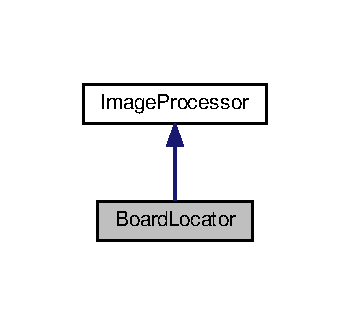
\includegraphics[width=168pt]{classBoardLocator__inherit__graph}
\end{center}
\end{figure}


Collaboration diagram for Board\+Locator\+:\nopagebreak
\begin{figure}[H]
\begin{center}
\leavevmode
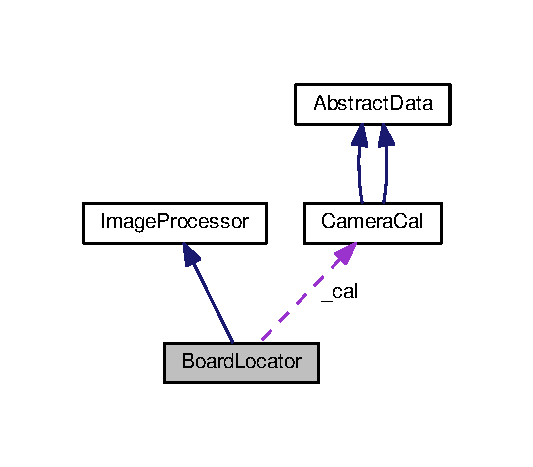
\includegraphics[width=256pt]{classBoardLocator__coll__graph}
\end{center}
\end{figure}
\subsection*{Public Member Functions}
\begin{DoxyCompactItemize}
\item 
void {\bfseries set\+Output\+Dir} (boost\+::filesystem\+::path dir)\hypertarget{classBoardLocator_afec0b2b2ed20d6d88df974cb70dd9068}{}\label{classBoardLocator_afec0b2b2ed20d6d88df974cb70dd9068}

\item 
void {\bfseries save} ()\hypertarget{classBoardLocator_aa2aa939df52f013a6b1536349cad40c6}{}\label{classBoardLocator_aa2aa939df52f013a6b1536349cad40c6}

\item 
void {\bfseries set\+List} (std\+::shared\+\_\+ptr$<$ \hyperlink{classImageList}{Image\+List}$<$ \hyperlink{classImage}{Image} $>$ $>$ in\+List, std\+::shared\+\_\+ptr$<$ \hyperlink{classImageList}{Image\+List}$<$ \hyperlink{classImage}{Image} $>$ $>$ out\+List)\hypertarget{classBoardLocator_ab2c61c79c92766cb63b2c88709f9ddb9}{}\label{classBoardLocator_ab2c61c79c92766cb63b2c88709f9ddb9}

\item 
void {\bfseries set\+Camera\+Cal} (\hyperlink{classCameraCal}{Camera\+Cal} cal)\hypertarget{classBoardLocator_a2711154066601fa30ea260b5f063ea34}{}\label{classBoardLocator_a2711154066601fa30ea260b5f063ea34}

\item 
void {\bfseries setup\+Board} (int num\+Horizontal, int num\+Vertical, float cell\+Dim)\hypertarget{classBoardLocator_aed856a6d3da376ef415f06fa58436be0}{}\label{classBoardLocator_aed856a6d3da376ef415f06fa58436be0}

\item 
void {\bfseries set\+Min\+Board} (int row, int col)\hypertarget{classBoardLocator_a975c6ea16a45ecbe1db48494beeb1f38}{}\label{classBoardLocator_a975c6ea16a45ecbe1db48494beeb1f38}

\item 
\hyperlink{classautoSizeBoard}{auto\+Size\+Board} \& {\bfseries get\+Board} (unsigned int i)\hypertarget{classBoardLocator_af5516dabace68531b4723e807916f630}{}\label{classBoardLocator_af5516dabace68531b4723e807916f630}

\item 
void {\bfseries find\+Board} (unsigned int i)\hypertarget{classBoardLocator_a90d2b37d862f255be0d8de4a8eb68764}{}\label{classBoardLocator_a90d2b37d862f255be0d8de4a8eb68764}

\end{DoxyCompactItemize}
\subsection*{Protected Member Functions}
\begin{DoxyCompactItemize}
\item 
void {\bfseries run\+Operations} ()\hypertarget{classBoardLocator_a08ec97bb3b5a5228c8e9090d525c2816}{}\label{classBoardLocator_a08ec97bb3b5a5228c8e9090d525c2816}

\end{DoxyCompactItemize}
\subsection*{Protected Attributes}
\begin{DoxyCompactItemize}
\item 
boost\+::filesystem\+::path {\bfseries \+\_\+save\+Path}\hypertarget{classBoardLocator_a80885202ff22cfc4fee337d29c61047b}{}\label{classBoardLocator_a80885202ff22cfc4fee337d29c61047b}

\item 
std\+::vector$<$ \hyperlink{classautoSizeBoard}{auto\+Size\+Board} $>$ {\bfseries \+\_\+boards}\hypertarget{classBoardLocator_a486f5e1573f84e3c8af5169855e4909c}{}\label{classBoardLocator_a486f5e1573f84e3c8af5169855e4909c}

\item 
\hyperlink{classCameraCal}{Camera\+Cal} {\bfseries \+\_\+cal}\hypertarget{classBoardLocator_a608463a44ef3dd90634277115203bd61}{}\label{classBoardLocator_a608463a44ef3dd90634277115203bd61}

\item 
int {\bfseries \+\_\+num\+Horizontal}\hypertarget{classBoardLocator_a5fe2fc7e06c6774bf195ab0a05282dac}{}\label{classBoardLocator_a5fe2fc7e06c6774bf195ab0a05282dac}

\item 
int {\bfseries \+\_\+num\+Vertical}\hypertarget{classBoardLocator_a80b5c8ff6a8f3b7aea19ef3545fa487c}{}\label{classBoardLocator_a80b5c8ff6a8f3b7aea19ef3545fa487c}

\item 
float {\bfseries \+\_\+cell\+Dim}\hypertarget{classBoardLocator_a79404e4c68c077a5eac599fb7e7c2c90}{}\label{classBoardLocator_a79404e4c68c077a5eac599fb7e7c2c90}

\item 
int {\bfseries \+\_\+row}\hypertarget{classBoardLocator_a4d3182d946b8b3baa1f9662e82a50190}{}\label{classBoardLocator_a4d3182d946b8b3baa1f9662e82a50190}

\item 
int {\bfseries \+\_\+col}\hypertarget{classBoardLocator_aaf12e063957845af1561ca008f92de4e}{}\label{classBoardLocator_aaf12e063957845af1561ca008f92de4e}

\end{DoxyCompactItemize}


The documentation for this class was generated from the following files\+:\begin{DoxyCompactItemize}
\item 
/home/labrat/\+Desktop/cam-\/proc/src/camera\+Cal2/src/boardlocator.\+h\item 
/home/labrat/\+Desktop/cam-\/proc/src/camera\+Cal2/src/boardlocator.\+cpp\end{DoxyCompactItemize}

\hypertarget{classcalibrator2d}{}\section{calibrator2d Class Reference}
\label{classcalibrator2d}\index{calibrator2d@{calibrator2d}}


Collaboration diagram for calibrator2d\+:\nopagebreak
\begin{figure}[H]
\begin{center}
\leavevmode
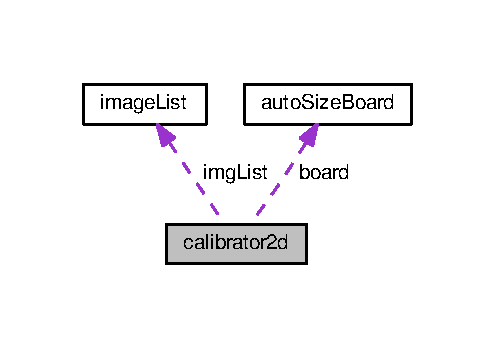
\includegraphics[width=238pt]{classcalibrator2d__coll__graph}
\end{center}
\end{figure}
\subsection*{Public Member Functions}
\begin{DoxyCompactItemize}
\item 
void {\bfseries setup\+Board} (int num\+Horizontal, int num\+Vertical, float grid\+Size)\hypertarget{classcalibrator2d_af7ea8fea2fe2f4dddaabf53eaeb627f0}{}\label{classcalibrator2d_af7ea8fea2fe2f4dddaabf53eaeb627f0}

\item 
void {\bfseries setup\+Asym\+Circ\+Board} (int num\+Horizontal, int num\+Vertical, float grid\+Size)\hypertarget{classcalibrator2d_a054356794a38491ec50d5f00de6921d8}{}\label{classcalibrator2d_a054356794a38491ec50d5f00de6921d8}

\item 
bool {\bfseries find\+Corners} ()\hypertarget{classcalibrator2d_ae21a633c8fdbc9d1d985780100688147}{}\label{classcalibrator2d_ae21a633c8fdbc9d1d985780100688147}

\item 
bool {\bfseries store\+Points} ()\hypertarget{classcalibrator2d_a9c7c8404911a25bca21ea6ee03152528}{}\label{classcalibrator2d_a9c7c8404911a25bca21ea6ee03152528}

\item 
bool {\bfseries unstore\+Points} ()\hypertarget{classcalibrator2d_abe2a5a7eb62731f43f6f8343ab37aa15}{}\label{classcalibrator2d_abe2a5a7eb62731f43f6f8343ab37aa15}

\item 
void {\bfseries calibrate} ()\hypertarget{classcalibrator2d_ac25ed63af6de3722155eda9b0844f977}{}\label{classcalibrator2d_ac25ed63af6de3722155eda9b0844f977}

\item 
void {\bfseries undistort\+Image} ()\hypertarget{classcalibrator2d_a96d83df2b7d366d42bf61547358c9af5}{}\label{classcalibrator2d_a96d83df2b7d366d42bf61547358c9af5}

\item 
bool {\bfseries next\+Image} ()\hypertarget{classcalibrator2d_a2d7e0a23afbc322ca77d628f34ab0613}{}\label{classcalibrator2d_a2d7e0a23afbc322ca77d628f34ab0613}

\item 
bool {\bfseries prev\+Image} ()\hypertarget{classcalibrator2d_af1a3bf827f11c6737b8369eae4789c62}{}\label{classcalibrator2d_af1a3bf827f11c6737b8369eae4789c62}

\item 
void {\bfseries goto\+Image} (int index)\hypertarget{classcalibrator2d_a9fd8b766132a7ce73343865ec06fcc0c}{}\label{classcalibrator2d_a9fd8b766132a7ce73343865ec06fcc0c}

\item 
int {\bfseries get\+Index} ()\hypertarget{classcalibrator2d_a4fa946638fe84cb015904af249d383c8}{}\label{classcalibrator2d_a4fa946638fe84cb015904af249d383c8}

\item 
\hyperlink{classcalImage}{cal\+Image} {\bfseries get\+Image} ()\hypertarget{classcalibrator2d_aebf7e6f254b50edef6dadea24d7095ce}{}\label{classcalibrator2d_aebf7e6f254b50edef6dadea24d7095ce}

\item 
\hyperlink{classcalImage}{cal\+Image} {\bfseries get\+Image} (int index)\hypertarget{classcalibrator2d_a73eb66d400663b1693188c9798364773}{}\label{classcalibrator2d_a73eb66d400663b1693188c9798364773}

\item 
double {\bfseries compute\+Reprojection\+Errors} ()\hypertarget{classcalibrator2d_a7cc23e9a343e0acef95e6b83dda108fd}{}\label{classcalibrator2d_a7cc23e9a343e0acef95e6b83dda108fd}

\item 
vector$<$ vector$<$ Point3f $>$ $>$ {\bfseries get\+Object\+Point\+Vect} ()\hypertarget{classcalibrator2d_a4e1d16dcb976d268985032a42bf627ad}{}\label{classcalibrator2d_a4e1d16dcb976d268985032a42bf627ad}

\item 
vector$<$ vector$<$ Point2f $>$ $>$ {\bfseries get\+Image\+Point\+Vect} ()\hypertarget{classcalibrator2d_a3861a75680988cb9bb098832faba0133}{}\label{classcalibrator2d_a3861a75680988cb9bb098832faba0133}

\item 
\hyperlink{classcalImage}{cal\+Image} \& {\bfseries current\+Image} ()\hypertarget{classcalibrator2d_a5e693cda283906f1077e89117c11a34c}{}\label{classcalibrator2d_a5e693cda283906f1077e89117c11a34c}

\item 
void {\bfseries write\+Y\+A\+ML} (string Filename)\hypertarget{classcalibrator2d_ace320844475a379524b8dd18ff037036}{}\label{classcalibrator2d_ace320844475a379524b8dd18ff037036}

\item 
Mat {\bfseries get\+Image\+Undistorted} ()\hypertarget{classcalibrator2d_a679d99c79f8a8d499a896c60e1734f20}{}\label{classcalibrator2d_a679d99c79f8a8d499a896c60e1734f20}

\item 
bool {\bfseries is\+Calibrated} ()\hypertarget{classcalibrator2d_a3e84790c9d4fcd23202f02b3d6917f5d}{}\label{classcalibrator2d_a3e84790c9d4fcd23202f02b3d6917f5d}

\item 
Mat {\bfseries get\+Board\+Position} (\hyperlink{classcalImage}{cal\+Image} image)\hypertarget{classcalibrator2d_addc5eb020d5b77d46dcc9cc3a6e619cf}{}\label{classcalibrator2d_addc5eb020d5b77d46dcc9cc3a6e619cf}

\end{DoxyCompactItemize}
\subsection*{Public Attributes}
\begin{DoxyCompactItemize}
\item 
string {\bfseries name}\hypertarget{classcalibrator2d_a88560863cdfd0d2e43e44e6b241dc505}{}\label{classcalibrator2d_a88560863cdfd0d2e43e44e6b241dc505}

\item 
int {\bfseries num\+Boards}\hypertarget{classcalibrator2d_abe280c775f9ba89aae38d95435d3a6da}{}\label{classcalibrator2d_abe280c775f9ba89aae38d95435d3a6da}

\item 
int {\bfseries num\+Corners\+Hor}\hypertarget{classcalibrator2d_aa538c957784bdff0ba0c84cdc34e8f92}{}\label{classcalibrator2d_aa538c957784bdff0ba0c84cdc34e8f92}

\item 
int {\bfseries num\+Corners\+Ver}\hypertarget{classcalibrator2d_a2f7c137e6f18e1df5702c4b4d21a0040}{}\label{classcalibrator2d_a2f7c137e6f18e1df5702c4b4d21a0040}

\item 
int {\bfseries current\+Index}\hypertarget{classcalibrator2d_a85569cbf4f68929d9989c57c3f9c9bea}{}\label{classcalibrator2d_a85569cbf4f68929d9989c57c3f9c9bea}

\item 
\hyperlink{classautoSizeBoard}{auto\+Size\+Board} {\bfseries board}\hypertarget{classcalibrator2d_a54283621abdd58143b09ef4356c4b081}{}\label{classcalibrator2d_a54283621abdd58143b09ef4356c4b081}

\item 
int {\bfseries num\+Squares}\hypertarget{classcalibrator2d_a65b53307b8031572b5a819581e1a2e8a}{}\label{classcalibrator2d_a65b53307b8031572b5a819581e1a2e8a}

\item 
Size {\bfseries board\+\_\+sz}\hypertarget{classcalibrator2d_a1a9af4fba61d04293e061956e3349c78}{}\label{classcalibrator2d_a1a9af4fba61d04293e061956e3349c78}

\item 
\hyperlink{classimageList}{image\+List} {\bfseries img\+List}\hypertarget{classcalibrator2d_a612fa12b74f6ef630b49155e4f576f52}{}\label{classcalibrator2d_a612fa12b74f6ef630b49155e4f576f52}

\item 
vector$<$ Point2f $>$ {\bfseries corners}\hypertarget{classcalibrator2d_adb97aedf68f6c16c34270e70cf92d202}{}\label{classcalibrator2d_adb97aedf68f6c16c34270e70cf92d202}

\item 
int {\bfseries successes}\hypertarget{classcalibrator2d_a37a24fb3cef873171c031aeca8111a5c}{}\label{classcalibrator2d_a37a24fb3cef873171c031aeca8111a5c}

\item 
Mat {\bfseries intrinsic}\hypertarget{classcalibrator2d_a75914e9fea74ae658e6e3a7f9481cf8c}{}\label{classcalibrator2d_a75914e9fea74ae658e6e3a7f9481cf8c}

\item 
Mat {\bfseries dist\+Coeffs}\hypertarget{classcalibrator2d_ab179ebea2e60550d890bd0aeb3bd6510}{}\label{classcalibrator2d_ab179ebea2e60550d890bd0aeb3bd6510}

\item 
vector$<$ Mat $>$ {\bfseries rvecs}\hypertarget{classcalibrator2d_a58a3c5ca197092e320f4faeced4e26c5}{}\label{classcalibrator2d_a58a3c5ca197092e320f4faeced4e26c5}

\item 
vector$<$ Mat $>$ {\bfseries tvecs}\hypertarget{classcalibrator2d_afcd4858c26c63659ea2f59653f044b7c}{}\label{classcalibrator2d_afcd4858c26c63659ea2f59653f044b7c}

\item 
double {\bfseries fovx}\hypertarget{classcalibrator2d_ab620f4085345c447c5680e51b6bbbb17}{}\label{classcalibrator2d_ab620f4085345c447c5680e51b6bbbb17}

\item 
double {\bfseries fovy}\hypertarget{classcalibrator2d_acf74a3b93886b97c4e8a4784bef34bc9}{}\label{classcalibrator2d_acf74a3b93886b97c4e8a4784bef34bc9}

\item 
double {\bfseries focal\+Length}\hypertarget{classcalibrator2d_a6a1758714a608f3a9b24ec2f2b870acd}{}\label{classcalibrator2d_a6a1758714a608f3a9b24ec2f2b870acd}

\item 
Point2d {\bfseries principal\+Point}\hypertarget{classcalibrator2d_af7316fcff2d727265af2cea6e87edbc5}{}\label{classcalibrator2d_af7316fcff2d727265af2cea6e87edbc5}

\item 
Mat {\bfseries rectification}\hypertarget{classcalibrator2d_a00ce904d0010879ed738efee7738e51a}{}\label{classcalibrator2d_a00ce904d0010879ed738efee7738e51a}

\item 
Mat {\bfseries projection}\hypertarget{classcalibrator2d_a6818a2c5dd7db159bc06e7a1b4c362b2}{}\label{classcalibrator2d_a6818a2c5dd7db159bc06e7a1b4c362b2}

\item 
Mat {\bfseries mapX}\hypertarget{classcalibrator2d_adc87f58a631730999b9b02567796faba}{}\label{classcalibrator2d_adc87f58a631730999b9b02567796faba}

\item 
Mat {\bfseries mapY}\hypertarget{classcalibrator2d_a55c46dbb0e93fa42dc9ab53e91a893a7}{}\label{classcalibrator2d_a55c46dbb0e93fa42dc9ab53e91a893a7}

\item 
Mat {\bfseries imgU}\hypertarget{classcalibrator2d_a41559c6c5924c0df9bfda1ce354d9f03}{}\label{classcalibrator2d_a41559c6c5924c0df9bfda1ce354d9f03}

\item 
vector$<$ float $>$ {\bfseries per\+View\+Errors}\hypertarget{classcalibrator2d_a66bff8908a002c37e915454b99b0738d}{}\label{classcalibrator2d_a66bff8908a002c37e915454b99b0738d}

\item 
vector$<$ vector$<$ double $>$ $>$ {\bfseries per\+ViewX}\hypertarget{classcalibrator2d_aa8bd4480acaf1cb660f1c28b60f2da28}{}\label{classcalibrator2d_aa8bd4480acaf1cb660f1c28b60f2da28}

\item 
vector$<$ vector$<$ double $>$ $>$ {\bfseries per\+ViewY}\hypertarget{classcalibrator2d_a9f423a039647698693269ec55d63cdd9}{}\label{classcalibrator2d_a9f423a039647698693269ec55d63cdd9}

\item 
double {\bfseries total\+Error}\hypertarget{classcalibrator2d_a77f577df3c8ad43cab3d751c621188e5}{}\label{classcalibrator2d_a77f577df3c8ad43cab3d751c621188e5}

\end{DoxyCompactItemize}


The documentation for this class was generated from the following files\+:\begin{DoxyCompactItemize}
\item 
/home/labrat/\+Desktop/cam-\/proc/src/camera\+Calibration/calibrator2d.\+h\item 
/home/labrat/\+Desktop/cam-\/proc/src/camera\+Calibration/calibrator2d.\+cpp\end{DoxyCompactItemize}

\hypertarget{classcalibrator3d}{}\section{calibrator3d Class Reference}
\label{classcalibrator3d}\index{calibrator3d@{calibrator3d}}
\subsection*{Public Member Functions}
\begin{DoxyCompactItemize}
\item 
void {\bfseries setup\+Board} (int num\+Horizontal, int num\+Vertical, float grid\+Size)\hypertarget{classcalibrator3d_aecb62318e30c38f8b2204596ea9ec9ee}{}\label{classcalibrator3d_aecb62318e30c38f8b2204596ea9ec9ee}

\item 
bool {\bfseries find\+Corners} ()\hypertarget{classcalibrator3d_ab9d0a808ef3aa58e82079b6f97e512b0}{}\label{classcalibrator3d_ab9d0a808ef3aa58e82079b6f97e512b0}

\item 
bool {\bfseries store\+Points} ()\hypertarget{classcalibrator3d_af42cc19f1960c3a56dcb7f9ccdfeae29}{}\label{classcalibrator3d_af42cc19f1960c3a56dcb7f9ccdfeae29}

\item 
bool {\bfseries unstore\+Points} ()\hypertarget{classcalibrator3d_a46bdca4abe7a6e489092d01c85616211}{}\label{classcalibrator3d_a46bdca4abe7a6e489092d01c85616211}

\item 
void {\bfseries calibrate} ()\hypertarget{classcalibrator3d_a80e384f11c6a626ecc2872de97bf1724}{}\label{classcalibrator3d_a80e384f11c6a626ecc2872de97bf1724}

\item 
void {\bfseries write\+Y\+A\+ML} (string Filename)\hypertarget{classcalibrator3d_ab6ec3752c125a089ee5c595fce7d8e43}{}\label{classcalibrator3d_ab6ec3752c125a089ee5c595fce7d8e43}

\item 
void {\bfseries undistort\+Image} ()\hypertarget{classcalibrator3d_a52aa09a9535d0d59134bb2d552b14b50}{}\label{classcalibrator3d_a52aa09a9535d0d59134bb2d552b14b50}

\item 
void {\bfseries set\+Image} (int cam, Mat img)\hypertarget{classcalibrator3d_aada8c2f3bd578c79892ab90a3a443aa2}{}\label{classcalibrator3d_aada8c2f3bd578c79892ab90a3a443aa2}

\item 
\hyperlink{classcalImage}{cal\+Image} {\bfseries get\+Image} (int cam, int index)\hypertarget{classcalibrator3d_ac27182045d9ac747149a18ca1f48b644}{}\label{classcalibrator3d_ac27182045d9ac747149a18ca1f48b644}

\item 
\hyperlink{classcalImage}{cal\+Image} {\bfseries get\+Image} (int cam)\hypertarget{classcalibrator3d_aba41be909e1c63e718a57e94aeda4296}{}\label{classcalibrator3d_aba41be909e1c63e718a57e94aeda4296}

\item 
bool {\bfseries next\+Image} ()\hypertarget{classcalibrator3d_a21bfd66de8a89b4558b90ba77544417f}{}\label{classcalibrator3d_a21bfd66de8a89b4558b90ba77544417f}

\item 
bool {\bfseries prev\+Image} ()\hypertarget{classcalibrator3d_a7f40bb67446f78cfda48b566bb808c10}{}\label{classcalibrator3d_a7f40bb67446f78cfda48b566bb808c10}

\item 
void {\bfseries goto\+Image} (int index)\hypertarget{classcalibrator3d_a3f0c08b97eb5160eeee236e1752fdae0}{}\label{classcalibrator3d_a3f0c08b97eb5160eeee236e1752fdae0}

\item 
int {\bfseries get\+Index} ()\hypertarget{classcalibrator3d_aaee1a1f6b595dd24e1835117c5336552}{}\label{classcalibrator3d_aaee1a1f6b595dd24e1835117c5336552}

\item 
float {\bfseries compare\+Detected\+Boards} ()\hypertarget{classcalibrator3d_a97bb110d3a556aaf5b5a317f00063c9c}{}\label{classcalibrator3d_a97bb110d3a556aaf5b5a317f00063c9c}

\end{DoxyCompactItemize}
\subsection*{Public Attributes}
\begin{DoxyCompactItemize}
\item 
vector$<$ \hyperlink{classcalibrator2d}{calibrator2d} $>$ {\bfseries cals}\hypertarget{classcalibrator3d_a4b8160b2c6c63e36e7caca6c7c7cfd20}{}\label{classcalibrator3d_a4b8160b2c6c63e36e7caca6c7c7cfd20}

\item 
int {\bfseries current\+Index}\hypertarget{classcalibrator3d_a123b6e46f2c82eade099783c5f84f3c8}{}\label{classcalibrator3d_a123b6e46f2c82eade099783c5f84f3c8}

\item 
bool {\bfseries board\+Found}\hypertarget{classcalibrator3d_a074d9de4f674b7ad31134b6d667e48dc}{}\label{classcalibrator3d_a074d9de4f674b7ad31134b6d667e48dc}

\item 
bool {\bfseries board\+Match}\hypertarget{classcalibrator3d_a531d16869b1113de631e8337a26a445f}{}\label{classcalibrator3d_a531d16869b1113de631e8337a26a445f}

\item 
int {\bfseries successes}\hypertarget{classcalibrator3d_a99f1552b106064d2139286a2244d679d}{}\label{classcalibrator3d_a99f1552b106064d2139286a2244d679d}

\item 
double {\bfseries total\+Error}\hypertarget{classcalibrator3d_ad8f51a15aebf584d2f47a2db0ea66888}{}\label{classcalibrator3d_ad8f51a15aebf584d2f47a2db0ea66888}

\item 
bool {\bfseries calibrated}\hypertarget{classcalibrator3d_afa23b323b9331541cd178730a62ddd0b}{}\label{classcalibrator3d_afa23b323b9331541cd178730a62ddd0b}

\item 
Mat {\bfseries R}\hypertarget{classcalibrator3d_a2c86fd41c790b69943d0b9c0f8cdf748}{}\label{classcalibrator3d_a2c86fd41c790b69943d0b9c0f8cdf748}

\item 
Mat {\bfseries T}\hypertarget{classcalibrator3d_abc81d70f1cc72f72ca4725b822499f17}{}\label{classcalibrator3d_abc81d70f1cc72f72ca4725b822499f17}

\item 
Mat {\bfseries E}\hypertarget{classcalibrator3d_a433708cbf86b2538429fe482c4630f9e}{}\label{classcalibrator3d_a433708cbf86b2538429fe482c4630f9e}

\item 
Mat {\bfseries F}\hypertarget{classcalibrator3d_aa6a857d10361437976e6de1e194bd8b3}{}\label{classcalibrator3d_aa6a857d10361437976e6de1e194bd8b3}

\item 
Mat {\bfseries Q}\hypertarget{classcalibrator3d_a846de3ef785d34d958ede8ce24c8896b}{}\label{classcalibrator3d_a846de3ef785d34d958ede8ce24c8896b}

\end{DoxyCompactItemize}


The documentation for this class was generated from the following files\+:\begin{DoxyCompactItemize}
\item 
/home/labrat/\+Desktop/cam-\/proc/src/camera\+Calibration/calibrator3d.\+h\item 
/home/labrat/\+Desktop/cam-\/proc/src/camera\+Calibration/calibrator3d.\+cpp\end{DoxyCompactItemize}

\hypertarget{classcalImage}{}\section{cal\+Image Class Reference}
\label{classcalImage}\index{cal\+Image@{cal\+Image}}
\subsection*{Public Member Functions}
\begin{DoxyCompactItemize}
\item 
{\bfseries cal\+Image} (string f\+Name)\hypertarget{classcalImage_a3259ab84fa9fe3580ace31fcbf530355}{}\label{classcalImage_a3259ab84fa9fe3580ace31fcbf530355}

\item 
void {\bfseries load\+File} ()\hypertarget{classcalImage_a25a15922791df037d2bf8cbd1554caab}{}\label{classcalImage_a25a15922791df037d2bf8cbd1554caab}

\item 
Mat {\bfseries get\+Display\+Image} ()\hypertarget{classcalImage_a6b5eb7212ffa855e94b73c4db4299e7d}{}\label{classcalImage_a6b5eb7212ffa855e94b73c4db4299e7d}

\item 
void {\bfseries remove\+Top} ()\hypertarget{classcalImage_ac2405b1109353fbc18c5c52f95ecab02}{}\label{classcalImage_ac2405b1109353fbc18c5c52f95ecab02}

\item 
void {\bfseries remove\+Btm} ()\hypertarget{classcalImage_ac871f35ecbe839979420a3180ab449cf}{}\label{classcalImage_ac871f35ecbe839979420a3180ab449cf}

\item 
void {\bfseries remove\+Right} ()\hypertarget{classcalImage_afc32b4e199f9ede93c8caef1258a6808}{}\label{classcalImage_afc32b4e199f9ede93c8caef1258a6808}

\item 
void {\bfseries remove\+Left} ()\hypertarget{classcalImage_ae27dc9e5fc7a7568027674d6fd26d9b5}{}\label{classcalImage_ae27dc9e5fc7a7568027674d6fd26d9b5}

\end{DoxyCompactItemize}
\subsection*{Public Attributes}
\begin{DoxyCompactItemize}
\item 
string {\bfseries filename}\hypertarget{classcalImage_a8fd18e3c9e81289afacf67ce22e331e3}{}\label{classcalImage_a8fd18e3c9e81289afacf67ce22e331e3}

\item 
Mat {\bfseries raw\+Mat}\hypertarget{classcalImage_ae674e9be7d896119514a4ed145c80998}{}\label{classcalImage_ae674e9be7d896119514a4ed145c80998}

\item 
Mat {\bfseries corners\+Mat}\hypertarget{classcalImage_a4b6fd3a65815e477a9f193b1d85df0d9}{}\label{classcalImage_a4b6fd3a65815e477a9f193b1d85df0d9}

\item 
vector$<$ Point3f $>$ {\bfseries object\+Points}\hypertarget{classcalImage_a406fc0391ee929dfcf3e754030c6872c}{}\label{classcalImage_a406fc0391ee929dfcf3e754030c6872c}

\item 
vector$<$ Point2f $>$ {\bfseries image\+Points}\hypertarget{classcalImage_a89c04d6e73b4dd191012bdce26107d75}{}\label{classcalImage_a89c04d6e73b4dd191012bdce26107d75}

\item 
Size {\bfseries board\+Size}\hypertarget{classcalImage_a2f6a06bb79979d589a098e9c63747e39}{}\label{classcalImage_a2f6a06bb79979d589a098e9c63747e39}

\item 
bool {\bfseries stored}\hypertarget{classcalImage_a0aef3196e33b17f4d195112584c96a25}{}\label{classcalImage_a0aef3196e33b17f4d195112584c96a25}

\item 
bool {\bfseries calibrated}\hypertarget{classcalImage_af99b7ce653bf83e954cb7697383b5d1a}{}\label{classcalImage_af99b7ce653bf83e954cb7697383b5d1a}

\item 
bool {\bfseries board\+Found}\hypertarget{classcalImage_a0d0309664b85fcf317563ba06d1ad618}{}\label{classcalImage_a0d0309664b85fcf317563ba06d1ad618}

\item 
bool {\bfseries search\+Attempted}\hypertarget{classcalImage_aa4df698416085d78784de08c4d06f6a7}{}\label{classcalImage_aa4df698416085d78784de08c4d06f6a7}

\item 
int {\bfseries rescale}\hypertarget{classcalImage_ae560d69a693664c1e17ae504db1c87ea}{}\label{classcalImage_ae560d69a693664c1e17ae504db1c87ea}

\end{DoxyCompactItemize}


The documentation for this class was generated from the following files\+:\begin{DoxyCompactItemize}
\item 
/home/labrat/\+Desktop/cam-\/proc/src/camera\+Calibration/imagelist.\+h\item 
/home/labrat/\+Desktop/cam-\/proc/src/camera\+Calibration/imagelist.\+cpp\end{DoxyCompactItemize}

\hypertarget{classCameraCal}{}\section{Camera\+Cal Class Reference}
\label{classCameraCal}\index{Camera\+Cal@{Camera\+Cal}}


Inheritance diagram for Camera\+Cal\+:\nopagebreak
\begin{figure}[H]
\begin{center}
\leavevmode
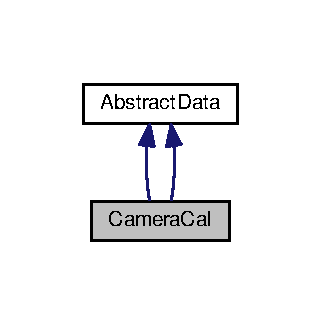
\includegraphics[width=154pt]{classCameraCal__inherit__graph}
\end{center}
\end{figure}


Collaboration diagram for Camera\+Cal\+:\nopagebreak
\begin{figure}[H]
\begin{center}
\leavevmode
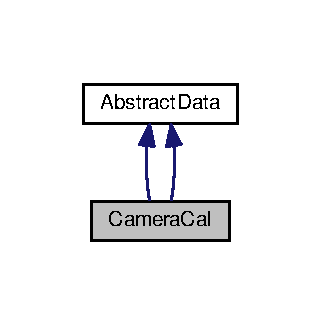
\includegraphics[width=154pt]{classCameraCal__coll__graph}
\end{center}
\end{figure}
\subsection*{Public Member Functions}
\begin{DoxyCompactItemize}
\item 
void \hyperlink{classCameraCal_a2f47fc4ab16adcdd6269184340e087ed}{read\+File} (std\+::string filename)
\begin{DoxyCompactList}\small\item\em abstract memeber to read data from a file using a filename \end{DoxyCompactList}\item 
void \hyperlink{classCameraCal_aed026a2f07ceffeaf5591072cae13f99}{write\+File} (std\+::string filename)
\begin{DoxyCompactList}\small\item\em abstract memeber to write data from a file using a filename \end{DoxyCompactList}\item 
void {\bfseries undistort\+Points} (cv\+::\+Mat \&input, cv\+::\+Mat \&output)\hypertarget{classCameraCal_a9190758a8a5759f1d6b312ad3d97a093}{}\label{classCameraCal_a9190758a8a5759f1d6b312ad3d97a093}

\item 
void {\bfseries undistort\+Points} (const std\+::vector$<$ float $>$ \&u\+In, const std\+::vector$<$ float $>$ \&v\+In, std\+::vector$<$ float $>$ \&u\+Out, std\+::vector$<$ float $>$ \&v\+Out)\hypertarget{classCameraCal_abdfe8dff383368dc307cac7428bc9ec3}{}\label{classCameraCal_abdfe8dff383368dc307cac7428bc9ec3}

\item 
void {\bfseries undistort\+Points} (const std\+::vector$<$ float $>$ \&u\+In, const std\+::vector$<$ float $>$ \&v\+In, cv\+::\+Mat \&output)\hypertarget{classCameraCal_afa30ca95ccf257c211274dc0ebc8d707}{}\label{classCameraCal_afa30ca95ccf257c211274dc0ebc8d707}

\item 
void \hyperlink{classCameraCal_aa1cc38014e07e74f9eaf139b72e55d09}{project\+Points} (std\+::vector$<$ cv\+::\+Point3f $>$ object\+Points, cv\+::\+Mat R, cv\+::\+Mat T, std\+::vector$<$ cv\+::\+Point2f $>$ \&output)
\begin{DoxyCompactList}\small\item\em \hyperlink{classCameraCal_aa1cc38014e07e74f9eaf139b72e55d09}{Camera\+Cal\+::project\+Points} Projects points from 3d space into the image frame. \end{DoxyCompactList}\item 
cv\+::\+Mat {\bfseries undistort\+Mat} (cv\+::\+Mat \&in)\hypertarget{classCameraCal_a61ac0d332a40375867c9f445e2bf62ce}{}\label{classCameraCal_a61ac0d332a40375867c9f445e2bf62ce}

\item 
\hyperlink{classImage}{Image} {\bfseries undistort\+Image} (\hyperlink{classImage}{Image} \&in)\hypertarget{classCameraCal_ad305161d3bb04ec8df1366d32dfd9c8d}{}\label{classCameraCal_ad305161d3bb04ec8df1366d32dfd9c8d}

\item 
void {\bfseries cam2world} (cv\+::\+Mat \&input\+Points, cv\+::\+Mat \&output\+Points)\hypertarget{classCameraCal_af768f460fecd28f833c6663c298719d4}{}\label{classCameraCal_af768f460fecd28f833c6663c298719d4}

\item 
void \hyperlink{classCameraCal_a2f47fc4ab16adcdd6269184340e087ed}{read\+File} (std\+::string filename)
\begin{DoxyCompactList}\small\item\em abstract memeber to read data from a file using a filename \end{DoxyCompactList}\item 
void \hyperlink{classCameraCal_aed026a2f07ceffeaf5591072cae13f99}{write\+File} (std\+::string filename)
\begin{DoxyCompactList}\small\item\em abstract memeber to write data from a file using a filename \end{DoxyCompactList}\item 
void {\bfseries undistort\+Points} (cv\+::\+Mat \&input, cv\+::\+Mat \&output)\hypertarget{classCameraCal_a9190758a8a5759f1d6b312ad3d97a093}{}\label{classCameraCal_a9190758a8a5759f1d6b312ad3d97a093}

\item 
void {\bfseries undistort\+Points} (const std\+::vector$<$ float $>$ \&u\+In, const std\+::vector$<$ float $>$ \&v\+In, std\+::vector$<$ float $>$ \&u\+Out, std\+::vector$<$ float $>$ \&v\+Out)\hypertarget{classCameraCal_abdfe8dff383368dc307cac7428bc9ec3}{}\label{classCameraCal_abdfe8dff383368dc307cac7428bc9ec3}

\item 
void {\bfseries undistort\+Points} (const std\+::vector$<$ float $>$ \&u\+In, const std\+::vector$<$ float $>$ \&v\+In, cv\+::\+Mat \&output)\hypertarget{classCameraCal_afa30ca95ccf257c211274dc0ebc8d707}{}\label{classCameraCal_afa30ca95ccf257c211274dc0ebc8d707}

\item 
cv\+::\+Mat {\bfseries undistort\+Mat} (cv\+::\+Mat \&in)\hypertarget{classCameraCal_a61ac0d332a40375867c9f445e2bf62ce}{}\label{classCameraCal_a61ac0d332a40375867c9f445e2bf62ce}

\item 
\hyperlink{classImage}{Image} {\bfseries undistort\+Image} (\hyperlink{classImage}{Image} \&in)\hypertarget{classCameraCal_ad305161d3bb04ec8df1366d32dfd9c8d}{}\label{classCameraCal_ad305161d3bb04ec8df1366d32dfd9c8d}

\item 
void {\bfseries cam2world} (cv\+::\+Mat \&input\+Points, cv\+::\+Mat \&output\+Points)\hypertarget{classCameraCal_af768f460fecd28f833c6663c298719d4}{}\label{classCameraCal_af768f460fecd28f833c6663c298719d4}

\end{DoxyCompactItemize}
\subsection*{Public Attributes}
\begin{DoxyCompactItemize}
\item 
std\+::string {\bfseries camera\+Name}\hypertarget{classCameraCal_a6b5eb4c36c863701cff34e9ba2d6f64b}{}\label{classCameraCal_a6b5eb4c36c863701cff34e9ba2d6f64b}

\item 
double {\bfseries reporjection\+Error}\hypertarget{classCameraCal_a7f1f8fbe6975378cc8ffec8338e379ba}{}\label{classCameraCal_a7f1f8fbe6975378cc8ffec8338e379ba}

\item 
cv\+::\+Mat {\bfseries camera\+Matrix}\hypertarget{classCameraCal_abe31c21ecea3289f2e103acb6cc1208a}{}\label{classCameraCal_abe31c21ecea3289f2e103acb6cc1208a}

\item 
cv\+::\+Mat {\bfseries dist\+Coeffs}\hypertarget{classCameraCal_a55d562412415e341ef76bcb9c80f67f4}{}\label{classCameraCal_a55d562412415e341ef76bcb9c80f67f4}

\item 
double {\bfseries fovx}\hypertarget{classCameraCal_ae2db6a3f823cc793317eae41c8681065}{}\label{classCameraCal_ae2db6a3f823cc793317eae41c8681065}

\item 
double {\bfseries fovy}\hypertarget{classCameraCal_a2348222df74031059d634835d5325411}{}\label{classCameraCal_a2348222df74031059d634835d5325411}

\item 
double {\bfseries focal\+Length}\hypertarget{classCameraCal_ae821e874698bde0d95f99bd80d9891af}{}\label{classCameraCal_ae821e874698bde0d95f99bd80d9891af}

\item 
cv\+::\+Point2d {\bfseries principal\+Point}\hypertarget{classCameraCal_a41774b2252dc7e1517728b579d0a48db}{}\label{classCameraCal_a41774b2252dc7e1517728b579d0a48db}

\end{DoxyCompactItemize}
\subsection*{Additional Inherited Members}


\subsection{Member Function Documentation}
\index{Camera\+Cal@{Camera\+Cal}!project\+Points@{project\+Points}}
\index{project\+Points@{project\+Points}!Camera\+Cal@{Camera\+Cal}}
\subsubsection[{\texorpdfstring{project\+Points(std\+::vector$<$ cv\+::\+Point3f $>$ object\+Points, cv\+::\+Mat R, cv\+::\+Mat T, std\+::vector$<$ cv\+::\+Point2f $>$ \&output)}{projectPoints(std::vector< cv::Point3f > objectPoints, cv::Mat R, cv::Mat T, std::vector< cv::Point2f > &output)}}]{\setlength{\rightskip}{0pt plus 5cm}void Camera\+Cal\+::project\+Points (
\begin{DoxyParamCaption}
\item[{std\+::vector$<$ cv\+::\+Point3f $>$}]{object\+Points, }
\item[{cv\+::\+Mat}]{R, }
\item[{cv\+::\+Mat}]{T, }
\item[{std\+::vector$<$ cv\+::\+Point2f $>$ \&}]{output}
\end{DoxyParamCaption}
)}\hypertarget{classCameraCal_aa1cc38014e07e74f9eaf139b72e55d09}{}\label{classCameraCal_aa1cc38014e07e74f9eaf139b72e55d09}


\hyperlink{classCameraCal_aa1cc38014e07e74f9eaf139b72e55d09}{Camera\+Cal\+::project\+Points} Projects points from 3d space into the image frame. 


\begin{DoxyParams}{Parameters}
{\em object\+Points} & the points in the the object (ie a checkerboard) \\
\hline
{\em R} & the rotation matrix of the object frame \\
\hline
{\em T} & the translation vector of the object frame \\
\hline
{\em output} & A referecne perameter that will be filled with the the points projected to the image frame; \\
\hline
\end{DoxyParams}
\index{Camera\+Cal@{Camera\+Cal}!read\+File@{read\+File}}
\index{read\+File@{read\+File}!Camera\+Cal@{Camera\+Cal}}
\subsubsection[{\texorpdfstring{read\+File(std\+::string filename)}{readFile(std::string filename)}}]{\setlength{\rightskip}{0pt plus 5cm}void Camera\+Cal\+::read\+File (
\begin{DoxyParamCaption}
\item[{std\+::string}]{filename}
\end{DoxyParamCaption}
)\hspace{0.3cm}{\ttfamily [virtual]}}\hypertarget{classCameraCal_a2f47fc4ab16adcdd6269184340e087ed}{}\label{classCameraCal_a2f47fc4ab16adcdd6269184340e087ed}


abstract memeber to read data from a file using a filename 


\begin{DoxyParams}{Parameters}
{\em filename} & the location of the file you wish to read from \\
\hline
\end{DoxyParams}
\begin{DoxyNote}{Note}
unless overridden this function will just print an error to the screen 
\end{DoxyNote}


Reimplemented from \hyperlink{classAbstractData_ab43309236fd644fd303b4b1468a87d86}{Abstract\+Data}.

\index{Camera\+Cal@{Camera\+Cal}!read\+File@{read\+File}}
\index{read\+File@{read\+File}!Camera\+Cal@{Camera\+Cal}}
\subsubsection[{\texorpdfstring{read\+File(std\+::string filename)}{readFile(std::string filename)}}]{\setlength{\rightskip}{0pt plus 5cm}void Camera\+Cal\+::read\+File (
\begin{DoxyParamCaption}
\item[{std\+::string}]{filename}
\end{DoxyParamCaption}
)\hspace{0.3cm}{\ttfamily [virtual]}}\hypertarget{classCameraCal_a2f47fc4ab16adcdd6269184340e087ed}{}\label{classCameraCal_a2f47fc4ab16adcdd6269184340e087ed}


abstract memeber to read data from a file using a filename 


\begin{DoxyParams}{Parameters}
{\em filename} & the location of the file you wish to read from \\
\hline
\end{DoxyParams}
\begin{DoxyNote}{Note}
unless overridden this function will just print an error to the screen 
\end{DoxyNote}


Reimplemented from \hyperlink{classAbstractData_ab43309236fd644fd303b4b1468a87d86}{Abstract\+Data}.

\index{Camera\+Cal@{Camera\+Cal}!write\+File@{write\+File}}
\index{write\+File@{write\+File}!Camera\+Cal@{Camera\+Cal}}
\subsubsection[{\texorpdfstring{write\+File(std\+::string filename)}{writeFile(std::string filename)}}]{\setlength{\rightskip}{0pt plus 5cm}void Camera\+Cal\+::write\+File (
\begin{DoxyParamCaption}
\item[{std\+::string}]{filename}
\end{DoxyParamCaption}
)\hspace{0.3cm}{\ttfamily [virtual]}}\hypertarget{classCameraCal_aed026a2f07ceffeaf5591072cae13f99}{}\label{classCameraCal_aed026a2f07ceffeaf5591072cae13f99}


abstract memeber to write data from a file using a filename 


\begin{DoxyParams}{Parameters}
{\em filename} & the location of the file you wish to write to \\
\hline
\end{DoxyParams}
\begin{DoxyNote}{Note}
unless overridden this function will just print an error to the screen 
\end{DoxyNote}


Reimplemented from \hyperlink{classAbstractData_a338dce47a9901032fd7b908a1c6df514}{Abstract\+Data}.

\index{Camera\+Cal@{Camera\+Cal}!write\+File@{write\+File}}
\index{write\+File@{write\+File}!Camera\+Cal@{Camera\+Cal}}
\subsubsection[{\texorpdfstring{write\+File(std\+::string filename)}{writeFile(std::string filename)}}]{\setlength{\rightskip}{0pt plus 5cm}void Camera\+Cal\+::write\+File (
\begin{DoxyParamCaption}
\item[{std\+::string}]{filename}
\end{DoxyParamCaption}
)\hspace{0.3cm}{\ttfamily [virtual]}}\hypertarget{classCameraCal_aed026a2f07ceffeaf5591072cae13f99}{}\label{classCameraCal_aed026a2f07ceffeaf5591072cae13f99}


abstract memeber to write data from a file using a filename 


\begin{DoxyParams}{Parameters}
{\em filename} & the location of the file you wish to write to \\
\hline
\end{DoxyParams}
\begin{DoxyNote}{Note}
unless overridden this function will just print an error to the screen 
\end{DoxyNote}


Reimplemented from \hyperlink{classAbstractData_a338dce47a9901032fd7b908a1c6df514}{Abstract\+Data}.



The documentation for this class was generated from the following files\+:\begin{DoxyCompactItemize}
\item 
/home/labrat/\+Desktop/cam-\/proc/src/camera\+Cal2/src/cameracal.\+h\item 
/home/labrat/\+Desktop/cam-\/proc/src/camera\+Cal2/src/cameracal.\+cpp\end{DoxyCompactItemize}

\hypertarget{classColorCorrector}{}\section{Color\+Corrector Class Reference}
\label{classColorCorrector}\index{Color\+Corrector@{Color\+Corrector}}


Inheritance diagram for Color\+Corrector\+:\nopagebreak
\begin{figure}[H]
\begin{center}
\leavevmode
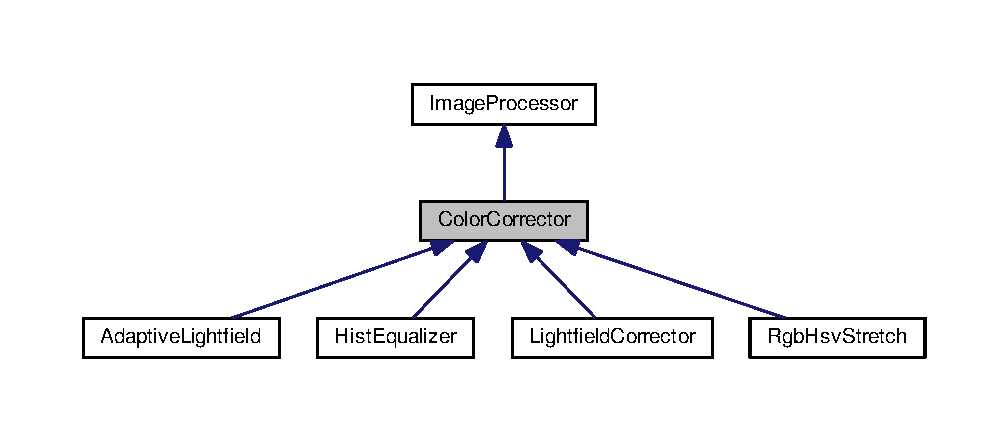
\includegraphics[width=350pt]{classColorCorrector__inherit__graph}
\end{center}
\end{figure}


Collaboration diagram for Color\+Corrector\+:\nopagebreak
\begin{figure}[H]
\begin{center}
\leavevmode
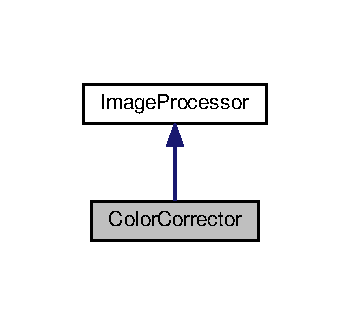
\includegraphics[width=168pt]{classColorCorrector__coll__graph}
\end{center}
\end{figure}
\subsection*{Additional Inherited Members}


The documentation for this class was generated from the following files\+:\begin{DoxyCompactItemize}
\item 
/home/labrat/\+Desktop/cam-\/proc/src/lib\+Cam/include/colorcorrector.\+h\item 
/home/labrat/\+Desktop/cam-\/proc/src/lib\+Cam/include/colorcorrector.\+cpp\end{DoxyCompactItemize}

\hypertarget{classconnectionBrowser}{}\section{connection\+Browser Class Reference}
\label{classconnectionBrowser}\index{connection\+Browser@{connection\+Browser}}


Inheritance diagram for connection\+Browser\+:
\nopagebreak
\begin{figure}[H]
\begin{center}
\leavevmode
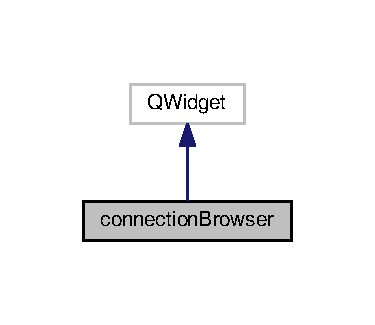
\includegraphics[width=180pt]{classconnectionBrowser__inherit__graph}
\end{center}
\end{figure}


Collaboration diagram for connection\+Browser\+:
\nopagebreak
\begin{figure}[H]
\begin{center}
\leavevmode
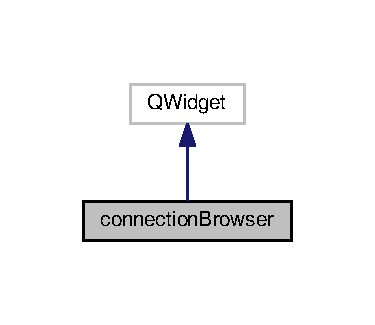
\includegraphics[width=180pt]{classconnectionBrowser__coll__graph}
\end{center}
\end{figure}
\subsection*{Public Member Functions}
\begin{DoxyCompactItemize}
\item 
{\bfseries connection\+Browser} (Q\+Widget $\ast$parent=nullptr)\hypertarget{classconnectionBrowser_a4d19db001fa9c839818765fdb2d88c58}{}\label{classconnectionBrowser_a4d19db001fa9c839818765fdb2d88c58}

\end{DoxyCompactItemize}


The documentation for this class was generated from the following files\+:\begin{DoxyCompactItemize}
\item 
/home/labrat/\+Desktop/cam-\/proc/src/lib\+Cam/qtinclude/connectionbrowser.\+h\item 
/home/labrat/\+Desktop/cam-\/proc/src/lib\+Cam/qtinclude/connectionbrowser.\+cpp\end{DoxyCompactItemize}

\hypertarget{classconnectionMenu}{}\section{connection\+Menu Class Reference}
\label{classconnectionMenu}\index{connection\+Menu@{connection\+Menu}}


Inheritance diagram for connection\+Menu\+:\nopagebreak
\begin{figure}[H]
\begin{center}
\leavevmode
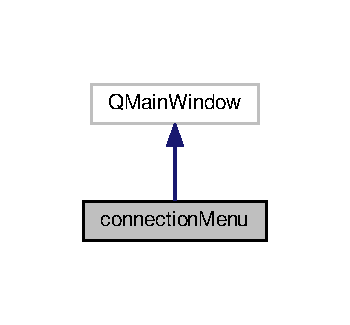
\includegraphics[width=168pt]{classconnectionMenu__inherit__graph}
\end{center}
\end{figure}


Collaboration diagram for connection\+Menu\+:\nopagebreak
\begin{figure}[H]
\begin{center}
\leavevmode
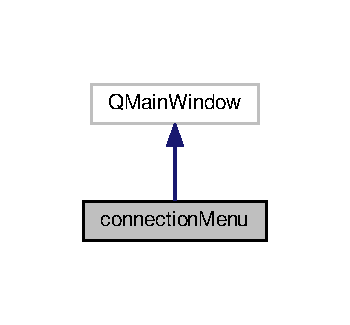
\includegraphics[width=168pt]{classconnectionMenu__coll__graph}
\end{center}
\end{figure}
\subsection*{Public Slots}
\begin{DoxyCompactItemize}
\item 
void {\bfseries refresh} ()\hypertarget{classconnectionMenu_a2ba8cffd81c1999c1dc02d3c915aa0fd}{}\label{classconnectionMenu_a2ba8cffd81c1999c1dc02d3c915aa0fd}

\item 
void {\bfseries show\+Meta\+Data} ()\hypertarget{classconnectionMenu_a4f1bc8eef79553047e8f00bbac27cb7b}{}\label{classconnectionMenu_a4f1bc8eef79553047e8f00bbac27cb7b}

\item 
void {\bfseries on\+\_\+tree\+Widget\+\_\+item\+Activated} (Q\+Tree\+Widget\+Item $\ast$\hyperlink{classitem}{item}, int column)\hypertarget{classconnectionMenu_aa51b970037b45ebdfe48efcb8d38fa23}{}\label{classconnectionMenu_aa51b970037b45ebdfe48efcb8d38fa23}

\item 
void {\bfseries on\+\_\+tree\+Widget\+\_\+current\+Item\+Changed} (Q\+Tree\+Widget\+Item $\ast$current, Q\+Tree\+Widget\+Item $\ast$previous)\hypertarget{classconnectionMenu_abfedee549afa5443963d10f9b5635e56}{}\label{classconnectionMenu_abfedee549afa5443963d10f9b5635e56}

\end{DoxyCompactItemize}
\subsection*{Signals}
\begin{DoxyCompactItemize}
\item 
void {\bfseries table\+Activated} (const Q\+String \&table)\hypertarget{classconnectionMenu_adfabb4075809b77b3c2ac9cd4188db35}{}\label{classconnectionMenu_adfabb4075809b77b3c2ac9cd4188db35}

\item 
void {\bfseries meta\+Data\+Requested} (const Q\+String \&table\+Name)\hypertarget{classconnectionMenu_ab48ece3cff2996fb996d05935211af0c}{}\label{classconnectionMenu_ab48ece3cff2996fb996d05935211af0c}

\end{DoxyCompactItemize}
\subsection*{Public Member Functions}
\begin{DoxyCompactItemize}
\item 
{\bfseries connection\+Menu} (Q\+Widget $\ast$parent=nullptr)\hypertarget{classconnectionMenu_aa87f3d2c274a8d29ed3c6dd553add391}{}\label{classconnectionMenu_aa87f3d2c274a8d29ed3c6dd553add391}

\item 
void {\bfseries set\+Output\+Images} (\hyperlink{classImageList}{Image\+List}$<$ \hyperlink{classImage}{Image} $>$\+::Ptr outimg)\hypertarget{classconnectionMenu_a6f950d2d62ea36a66b3a776b130635ab}{}\label{classconnectionMenu_a6f950d2d62ea36a66b3a776b130635ab}

\item 
Q\+String {\bfseries driver\+Name} () const \hypertarget{classconnectionMenu_aef48e171811f69a2bd079e8cd9db4ea2}{}\label{classconnectionMenu_aef48e171811f69a2bd079e8cd9db4ea2}

\item 
Q\+String {\bfseries database\+Name} () const \hypertarget{classconnectionMenu_a0f1d61138b91d54483d051151cf5b5f3}{}\label{classconnectionMenu_a0f1d61138b91d54483d051151cf5b5f3}

\item 
Q\+String {\bfseries user\+Name} () const \hypertarget{classconnectionMenu_ab9e9165781c77b19ba1a05a5a62c5b9c}{}\label{classconnectionMenu_ab9e9165781c77b19ba1a05a5a62c5b9c}

\item 
Q\+String {\bfseries password} () const \hypertarget{classconnectionMenu_afb7cbc2f5029567824451afcb5ba0206}{}\label{classconnectionMenu_afb7cbc2f5029567824451afcb5ba0206}

\item 
Q\+String {\bfseries host\+Name} () const \hypertarget{classconnectionMenu_a79d183c4750d3a2d4c1b3316b05ab1da}{}\label{classconnectionMenu_a79d183c4750d3a2d4c1b3316b05ab1da}

\item 
int {\bfseries port} () const \hypertarget{classconnectionMenu_a8f6a9bb6f4d515b068d2aacebd772c9f}{}\label{classconnectionMenu_a8f6a9bb6f4d515b068d2aacebd772c9f}

\item 
bool {\bfseries use\+In\+Memory\+Database} () const \hypertarget{classconnectionMenu_a38652ab512e0df213b9b13e1b21c2a2c}{}\label{classconnectionMenu_a38652ab512e0df213b9b13e1b21c2a2c}

\item 
Q\+Sql\+Database {\bfseries current\+Database} () const \hypertarget{classconnectionMenu_aaa8aaf26ba2626c8a3cc395e42bcd68c}{}\label{classconnectionMenu_aaa8aaf26ba2626c8a3cc395e42bcd68c}

\end{DoxyCompactItemize}


The documentation for this class was generated from the following files\+:\begin{DoxyCompactItemize}
\item 
/home/labrat/\+Desktop/cam-\/proc/src/lib\+Cam/qtinclude/connectionmenu.\+h\item 
/home/labrat/\+Desktop/cam-\/proc/src/lib\+Cam/qtinclude/connectionmenu.\+cpp\end{DoxyCompactItemize}

\hypertarget{classdataBase}{}\section{data\+Base Class Reference}
\label{classdataBase}\index{data\+Base@{data\+Base}}


Inheritance diagram for data\+Base\+:\nopagebreak
\begin{figure}[H]
\begin{center}
\leavevmode
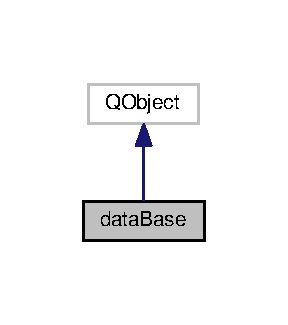
\includegraphics[width=138pt]{classdataBase__inherit__graph}
\end{center}
\end{figure}


Collaboration diagram for data\+Base\+:\nopagebreak
\begin{figure}[H]
\begin{center}
\leavevmode
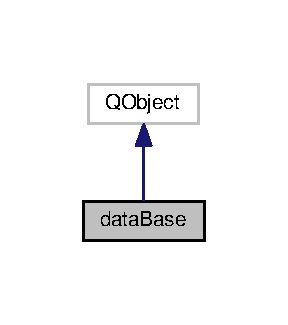
\includegraphics[width=138pt]{classdataBase__coll__graph}
\end{center}
\end{figure}
\subsection*{Public Member Functions}
\begin{DoxyCompactItemize}
\item 
{\bfseries data\+Base} (Q\+Object $\ast$parent=nullptr)\hypertarget{classdataBase_a53197521a30c3075260da045b7575f93}{}\label{classdataBase_a53197521a30c3075260da045b7575f93}

\item 
bool {\bfseries inizialization\+Data\+Base} (const Q\+String \&name\+Data\+Base)\hypertarget{classdataBase_a8f005ba00f5a3545baba1e304639bfbf}{}\label{classdataBase_a8f005ba00f5a3545baba1e304639bfbf}

\item 
bool {\bfseries configure\+Data\+Base} ()\hypertarget{classdataBase_ab1570d0f909bbb94288e87f1c9888929}{}\label{classdataBase_ab1570d0f909bbb94288e87f1c9888929}

\item 
Q\+String {\bfseries get\+Error} () const \hypertarget{classdataBase_a4c4bb9533d9f659d2fdc2d53f77b8ea0}{}\label{classdataBase_a4c4bb9533d9f659d2fdc2d53f77b8ea0}

\item 
bool {\bfseries add\+Item} (const \hyperlink{classitem}{item} \&items)\hypertarget{classdataBase_ab6e108898b0d9ddf48922457432e8b41}{}\label{classdataBase_ab6e108898b0d9ddf48922457432e8b41}

\end{DoxyCompactItemize}


The documentation for this class was generated from the following files\+:\begin{DoxyCompactItemize}
\item 
/home/labrat/\+Desktop/cam-\/proc/src/\+E\+R\+Database\+System/src/database.\+h\item 
/home/labrat/\+Desktop/cam-\/proc/src/\+E\+R\+Database\+System/src/database.\+cpp\end{DoxyCompactItemize}

\hypertarget{classdatabaseRoi}{}\section{database\+Roi Class Reference}
\label{classdatabaseRoi}\index{database\+Roi@{database\+Roi}}


Inheritance diagram for database\+Roi\+:\nopagebreak
\begin{figure}[H]
\begin{center}
\leavevmode
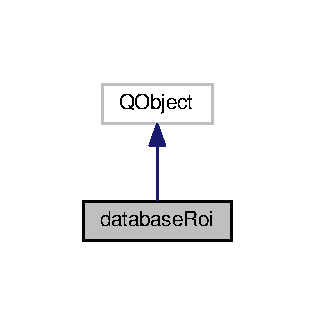
\includegraphics[width=151pt]{classdatabaseRoi__inherit__graph}
\end{center}
\end{figure}


Collaboration diagram for database\+Roi\+:\nopagebreak
\begin{figure}[H]
\begin{center}
\leavevmode
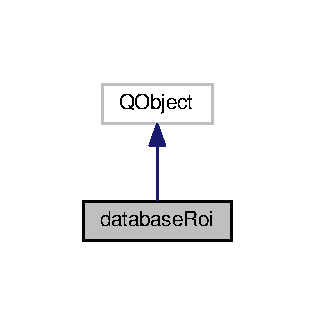
\includegraphics[width=151pt]{classdatabaseRoi__coll__graph}
\end{center}
\end{figure}
\subsection*{Public Member Functions}
\begin{DoxyCompactItemize}
\item 
{\bfseries database\+Roi} (Q\+Object $\ast$parent=nullptr)\hypertarget{classdatabaseRoi_a72439aded96c23105d78bb9461d3c60b}{}\label{classdatabaseRoi_a72439aded96c23105d78bb9461d3c60b}

\item 
bool {\bfseries inizialization\+Database\+Roi} (const Q\+String \&name\+Data\+Base)\hypertarget{classdatabaseRoi_a68f89be2b5aedfe17a5a0b7553f976f3}{}\label{classdatabaseRoi_a68f89be2b5aedfe17a5a0b7553f976f3}

\item 
bool {\bfseries configuration\+Database\+Roi} ()\hypertarget{classdatabaseRoi_a5a8aa4df2cae5ae3b8e7cfb863014d78}{}\label{classdatabaseRoi_a5a8aa4df2cae5ae3b8e7cfb863014d78}

\item 
Q\+String {\bfseries get\+Error} () const \hypertarget{classdatabaseRoi_a37fd6d6c60daca94cc9b4233ddcff017}{}\label{classdatabaseRoi_a37fd6d6c60daca94cc9b4233ddcff017}

\item 
bool {\bfseries add\+Item} (const \hyperlink{classitemRoi}{item\+Roi} $\ast$\hyperlink{classitem}{item})\hypertarget{classdatabaseRoi_a3746a6ef5f1d230d6c5a37a1f57df969}{}\label{classdatabaseRoi_a3746a6ef5f1d230d6c5a37a1f57df969}

\end{DoxyCompactItemize}


The documentation for this class was generated from the following files\+:\begin{DoxyCompactItemize}
\item 
/home/labrat/\+Desktop/cam-\/proc/src/\+E\+R\+Database\+System/src/databaseroi.\+h\item 
/home/labrat/\+Desktop/cam-\/proc/src/\+E\+R\+Database\+System/src/databaseroi.\+cpp\end{DoxyCompactItemize}

\hypertarget{classdatabaseSearch}{}\section{database\+Search Class Reference}
\label{classdatabaseSearch}\index{database\+Search@{database\+Search}}


Inheritance diagram for database\+Search\+:\nopagebreak
\begin{figure}[H]
\begin{center}
\leavevmode
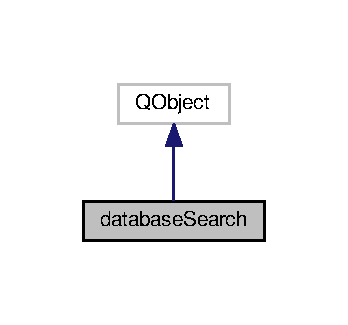
\includegraphics[width=167pt]{classdatabaseSearch__inherit__graph}
\end{center}
\end{figure}


Collaboration diagram for database\+Search\+:\nopagebreak
\begin{figure}[H]
\begin{center}
\leavevmode
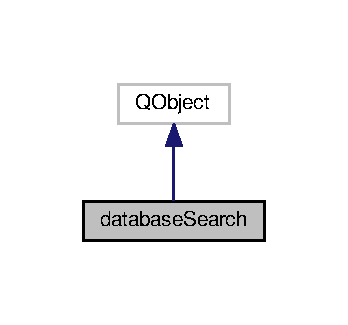
\includegraphics[width=167pt]{classdatabaseSearch__coll__graph}
\end{center}
\end{figure}
\subsection*{Public Member Functions}
\begin{DoxyCompactItemize}
\item 
{\bfseries database\+Search} (Q\+Object $\ast$parent=nullptr)\hypertarget{classdatabaseSearch_aae8e0eccc5ea8b298c0898468e72b542}{}\label{classdatabaseSearch_aae8e0eccc5ea8b298c0898468e72b542}

\item 
Q\+String {\bfseries get\+Error} () const \hypertarget{classdatabaseSearch_a2591c168f976c214de6112280df05fe5}{}\label{classdatabaseSearch_a2591c168f976c214de6112280df05fe5}

\item 
bool {\bfseries add\+Item} (const \hyperlink{classitemSearch}{item\+Search} \&\hyperlink{classitem}{item})\hypertarget{classdatabaseSearch_a97c19d28a7180382f7ec6e9d357a4d7e}{}\label{classdatabaseSearch_a97c19d28a7180382f7ec6e9d357a4d7e}

\end{DoxyCompactItemize}


The documentation for this class was generated from the following files\+:\begin{DoxyCompactItemize}
\item 
/home/labrat/\+Desktop/cam-\/proc/src/\+E\+R\+Database\+System/src/databasesearch.\+h\item 
/home/labrat/\+Desktop/cam-\/proc/src/\+E\+R\+Database\+System/src/databasesearch.\+cpp\end{DoxyCompactItemize}

\hypertarget{classedittabledialog}{}\section{edittabledialog Class Reference}
\label{classedittabledialog}\index{edittabledialog@{edittabledialog}}


Inheritance diagram for edittabledialog\+:\nopagebreak
\begin{figure}[H]
\begin{center}
\leavevmode
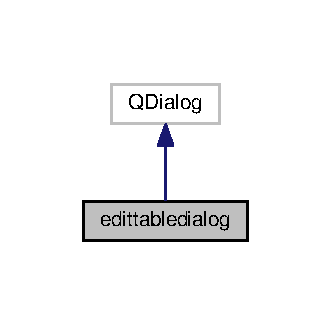
\includegraphics[width=159pt]{classedittabledialog__inherit__graph}
\end{center}
\end{figure}


Collaboration diagram for edittabledialog\+:\nopagebreak
\begin{figure}[H]
\begin{center}
\leavevmode
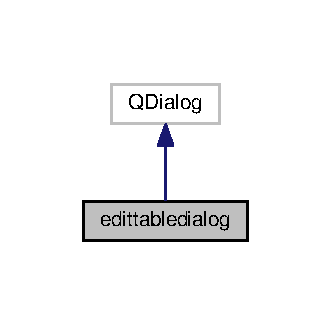
\includegraphics[width=159pt]{classedittabledialog__coll__graph}
\end{center}
\end{figure}
\subsection*{Public Member Functions}
\begin{DoxyCompactItemize}
\item 
{\bfseries edittabledialog} (const Q\+String \&table\+Name, Q\+Widget $\ast$parent=nullptr)\hypertarget{classedittabledialog_a8d51b98098349acbb11c8d3606f7bed2}{}\label{classedittabledialog_a8d51b98098349acbb11c8d3606f7bed2}

\end{DoxyCompactItemize}


The documentation for this class was generated from the following files\+:\begin{DoxyCompactItemize}
\item 
/home/labrat/\+Desktop/cam-\/proc/src/\+E\+R\+Database\+System/ui/edittabledialog.\+h\item 
/home/labrat/\+Desktop/cam-\/proc/src/\+E\+R\+Database\+System/ui/edittabledialog.\+cpp\end{DoxyCompactItemize}

\hypertarget{classERPreferencesDialog}{}\section{E\+R\+Preferences\+Dialog Class Reference}
\label{classERPreferencesDialog}\index{E\+R\+Preferences\+Dialog@{E\+R\+Preferences\+Dialog}}


Inheritance diagram for E\+R\+Preferences\+Dialog\+:\nopagebreak
\begin{figure}[H]
\begin{center}
\leavevmode
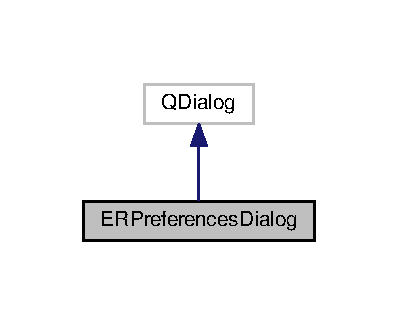
\includegraphics[width=191pt]{classERPreferencesDialog__inherit__graph}
\end{center}
\end{figure}


Collaboration diagram for E\+R\+Preferences\+Dialog\+:\nopagebreak
\begin{figure}[H]
\begin{center}
\leavevmode
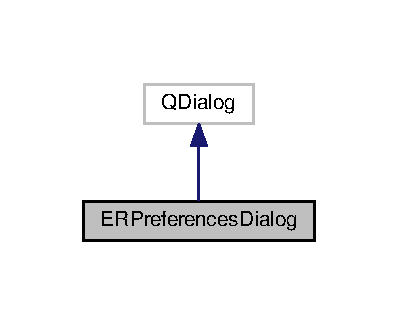
\includegraphics[width=191pt]{classERPreferencesDialog__coll__graph}
\end{center}
\end{figure}
\subsection*{Signals}
\begin{DoxyCompactItemize}
\item 
void {\bfseries font\+Selected} (Q\+Font)\hypertarget{classERPreferencesDialog_a3d144f0765745dc2eac4509f83e459d4}{}\label{classERPreferencesDialog_a3d144f0765745dc2eac4509f83e459d4}

\end{DoxyCompactItemize}
\subsection*{Public Member Functions}
\begin{DoxyCompactItemize}
\item 
{\bfseries E\+R\+Preferences\+Dialog} (Q\+Widget $\ast$parent=nullptr)\hypertarget{classERPreferencesDialog_aa29da15cfbe2a357aecb79f5e06f28ee}{}\label{classERPreferencesDialog_aa29da15cfbe2a357aecb79f5e06f28ee}

\end{DoxyCompactItemize}


The documentation for this class was generated from the following files\+:\begin{DoxyCompactItemize}
\item 
/home/labrat/\+Desktop/cam-\/proc/src/\+E\+R\+Database\+System/ui/erpreferencesdialog.\+h\item 
/home/labrat/\+Desktop/cam-\/proc/src/\+E\+R\+Database\+System/ui/erpreferencesdialog.\+cpp\end{DoxyCompactItemize}

\hypertarget{classERTreeWidget}{}\section{E\+R\+Tree\+Widget Class Reference}
\label{classERTreeWidget}\index{E\+R\+Tree\+Widget@{E\+R\+Tree\+Widget}}


Inheritance diagram for E\+R\+Tree\+Widget\+:\nopagebreak
\begin{figure}[H]
\begin{center}
\leavevmode
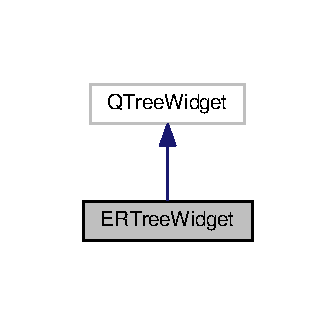
\includegraphics[width=161pt]{classERTreeWidget__inherit__graph}
\end{center}
\end{figure}


Collaboration diagram for E\+R\+Tree\+Widget\+:\nopagebreak
\begin{figure}[H]
\begin{center}
\leavevmode
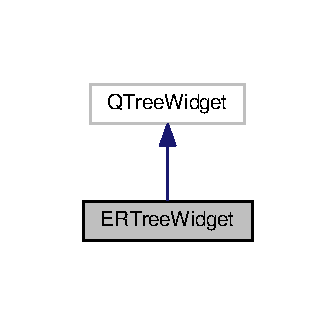
\includegraphics[width=161pt]{classERTreeWidget__coll__graph}
\end{center}
\end{figure}
\subsection*{Public Types}
\begin{DoxyCompactItemize}
\item 
enum {\bfseries Type} \{ {\bfseries N\+U\+L\+L\+P\+TR}, 
{\bfseries T\+A\+B\+LE}, 
{\bfseries B\+A\+SE}
 \}\hypertarget{classERTreeWidget_a45164f300024715be7e05e0424cf3978}{}\label{classERTreeWidget_a45164f300024715be7e05e0424cf3978}

\end{DoxyCompactItemize}
\subsection*{Signals}
\begin{DoxyCompactItemize}
\item 
void {\bfseries new\+Table} ()\hypertarget{classERTreeWidget_a58c1c59c25654e89556761adb57db518}{}\label{classERTreeWidget_a58c1c59c25654e89556761adb57db518}

\item 
void {\bfseries new\+Reference\+Table} ()\hypertarget{classERTreeWidget_a04d9ccc2dac42fb658860a0211bb9d46}{}\label{classERTreeWidget_a04d9ccc2dac42fb658860a0211bb9d46}

\item 
void {\bfseries remove\+Table} ()\hypertarget{classERTreeWidget_af3713c67d63adb1b909e377b2f5f5a42}{}\label{classERTreeWidget_af3713c67d63adb1b909e377b2f5f5a42}

\item 
void {\bfseries remove\+Database} ()\hypertarget{classERTreeWidget_a0e0c49fe2dbe0e1719fee91e84c5f8af}{}\label{classERTreeWidget_a0e0c49fe2dbe0e1719fee91e84c5f8af}

\item 
void {\bfseries select\+From} ()\hypertarget{classERTreeWidget_a4c4aa16739354a4f7dc499bf7c882971}{}\label{classERTreeWidget_a4c4aa16739354a4f7dc499bf7c882971}

\item 
void {\bfseries edit\+Table} ()\hypertarget{classERTreeWidget_ace19498a48a18de9c47cf0ddc881a9d1}{}\label{classERTreeWidget_ace19498a48a18de9c47cf0ddc881a9d1}

\end{DoxyCompactItemize}
\subsection*{Public Member Functions}
\begin{DoxyCompactItemize}
\item 
{\bfseries E\+R\+Tree\+Widget} (Q\+Widget $\ast$parent=nullptr)\hypertarget{classERTreeWidget_a4cdfac985b0386a7397ccadf8ff9a856}{}\label{classERTreeWidget_a4cdfac985b0386a7397ccadf8ff9a856}

\item 
Type {\bfseries type} (E\+R\+Tree\+Item $\ast$\hyperlink{classitem}{item}) const \hypertarget{classERTreeWidget_a5a5345b4b399db8379dd424af030ae15}{}\label{classERTreeWidget_a5a5345b4b399db8379dd424af030ae15}

\item 
Type {\bfseries type} () const \hypertarget{classERTreeWidget_af3bd5caed839e908692deff27072ec88}{}\label{classERTreeWidget_af3bd5caed839e908692deff27072ec88}

\end{DoxyCompactItemize}


The documentation for this class was generated from the following files\+:\begin{DoxyCompactItemize}
\item 
/home/labrat/\+Desktop/cam-\/proc/src/\+E\+R\+Database\+System/src/ertreewidget.\+h\item 
/home/labrat/\+Desktop/cam-\/proc/src/\+E\+R\+Database\+System/src/ertreewidget.\+cpp\end{DoxyCompactItemize}

\hypertarget{classFeatureExtractor}{}\section{Feature\+Extractor Class Reference}
\label{classFeatureExtractor}\index{Feature\+Extractor@{Feature\+Extractor}}


Inheritance diagram for Feature\+Extractor\+:\nopagebreak
\begin{figure}[H]
\begin{center}
\leavevmode
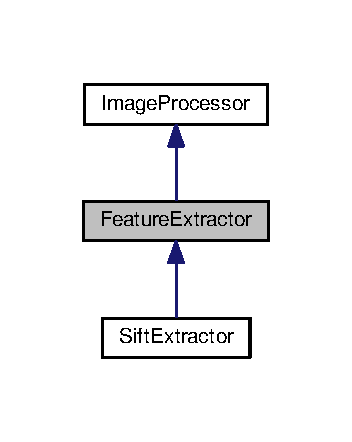
\includegraphics[width=169pt]{classFeatureExtractor__inherit__graph}
\end{center}
\end{figure}


Collaboration diagram for Feature\+Extractor\+:\nopagebreak
\begin{figure}[H]
\begin{center}
\leavevmode
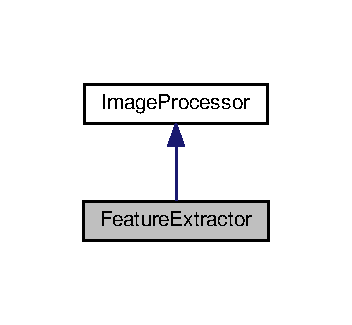
\includegraphics[width=169pt]{classFeatureExtractor__coll__graph}
\end{center}
\end{figure}
\subsection*{Public Member Functions}
\begin{DoxyCompactItemize}
\item 
const std\+::vector$<$ cv\+::\+Key\+Point $>$ \& {\bfseries get\+Keypoints} (unsigned int i)\hypertarget{classFeatureExtractor_af1efab93c025c4fa7702d5f3030162ca}{}\label{classFeatureExtractor_af1efab93c025c4fa7702d5f3030162ca}

\item 
const std\+::vector$<$ std\+::vector$<$ cv\+::\+Key\+Point $>$ $>$ \& {\bfseries get\+Keypoints\+Vect} ()\hypertarget{classFeatureExtractor_a4d60e9785ebdd8f3cd9ec4376b42c76a}{}\label{classFeatureExtractor_a4d60e9785ebdd8f3cd9ec4376b42c76a}

\item 
const cv\+::\+Mat {\bfseries get\+Descriptors} (unsigned int i)\hypertarget{classFeatureExtractor_ad66314da10ac655a7aa0a84240358e0a}{}\label{classFeatureExtractor_ad66314da10ac655a7aa0a84240358e0a}

\item 
const std\+::vector$<$ cv\+::\+Mat $>$ {\bfseries get\+Descriptors\+Vect} ()\hypertarget{classFeatureExtractor_a5993cd368b58cba1e4d7e1ebfba8150a}{}\label{classFeatureExtractor_a5993cd368b58cba1e4d7e1ebfba8150a}

\item 
void {\bfseries save} ()\hypertarget{classFeatureExtractor_a77bddef3bcc6abb2a8931234caeb78d1}{}\label{classFeatureExtractor_a77bddef3bcc6abb2a8931234caeb78d1}

\item 
virtual std\+::vector$<$ cv\+::\+Key\+Point $>$ {\bfseries get\+Features} (\hyperlink{classImage}{Image} \&in, cv\+::\+Mat \&descriptor)=0\hypertarget{classFeatureExtractor_a948b80d2c80b27d7a75332adb47495b0}{}\label{classFeatureExtractor_a948b80d2c80b27d7a75332adb47495b0}

\end{DoxyCompactItemize}
\subsection*{Protected Attributes}
\begin{DoxyCompactItemize}
\item 
std\+::vector$<$ std\+::vector$<$ cv\+::\+Key\+Point $>$ $>$ {\bfseries key\+Points}\hypertarget{classFeatureExtractor_aa3af21a7f3fa538dce8f66242d9ad58a}{}\label{classFeatureExtractor_aa3af21a7f3fa538dce8f66242d9ad58a}

\item 
std\+::vector$<$ cv\+::\+Mat $>$ {\bfseries descriptors}\hypertarget{classFeatureExtractor_a084b6eef4805aae1bc01568ae8420029}{}\label{classFeatureExtractor_a084b6eef4805aae1bc01568ae8420029}

\end{DoxyCompactItemize}
\subsection*{Additional Inherited Members}


The documentation for this class was generated from the following files\+:\begin{DoxyCompactItemize}
\item 
/home/labrat/\+Desktop/cam-\/proc/src/feature\+Extractor/featureextractor.\+h\item 
/home/labrat/\+Desktop/cam-\/proc/src/feature\+Extractor/featureextractor.\+cpp\end{DoxyCompactItemize}

\hypertarget{classFeatureMatcher}{}\section{Feature\+Matcher Class Reference}
\label{classFeatureMatcher}\index{Feature\+Matcher@{Feature\+Matcher}}


Inheritance diagram for Feature\+Matcher\+:\nopagebreak
\begin{figure}[H]
\begin{center}
\leavevmode
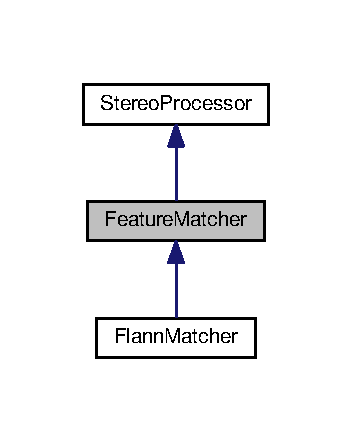
\includegraphics[width=169pt]{classFeatureMatcher__inherit__graph}
\end{center}
\end{figure}


Collaboration diagram for Feature\+Matcher\+:\nopagebreak
\begin{figure}[H]
\begin{center}
\leavevmode
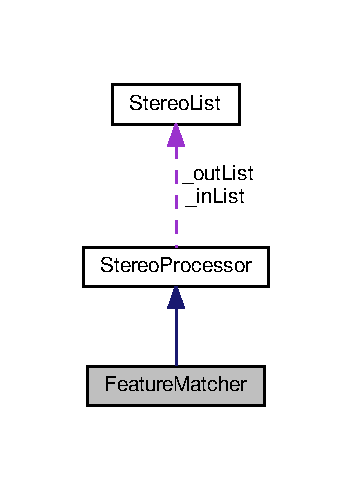
\includegraphics[width=169pt]{classFeatureMatcher__coll__graph}
\end{center}
\end{figure}
\subsection*{Public Member Functions}
\begin{DoxyCompactItemize}
\item 
{\bfseries Feature\+Matcher} (\hyperlink{classFeatureExtractor}{Feature\+Extractor} $\ast$a, \hyperlink{classFeatureExtractor}{Feature\+Extractor} $\ast$b)\hypertarget{classFeatureMatcher_a4ed4522a8ea2a0abfb4089ade947143a}{}\label{classFeatureMatcher_a4ed4522a8ea2a0abfb4089ade947143a}

\item 
std\+::shared\+\_\+ptr$<$ \hyperlink{classFeatureExtractor}{Feature\+Extractor} $>$ {\bfseries get\+ExtractorA} ()\hypertarget{classFeatureMatcher_a82d67143f4902c670faeafe6e2d07a2b}{}\label{classFeatureMatcher_a82d67143f4902c670faeafe6e2d07a2b}

\item 
std\+::shared\+\_\+ptr$<$ \hyperlink{classFeatureExtractor}{Feature\+Extractor} $>$ {\bfseries get\+ExtractorB} ()\hypertarget{classFeatureMatcher_a110a03a18df2c9b2c8db2b95b496d8ce}{}\label{classFeatureMatcher_a110a03a18df2c9b2c8db2b95b496d8ce}

\item 
void {\bfseries set\+Stereo\+List} (\hyperlink{classStereoList}{Stereo\+List} in\+List, \hyperlink{classStereoList}{Stereo\+List} out\+List)\hypertarget{classFeatureMatcher_a926e27d29ed7d9a3af6e2a056e28e24f}{}\label{classFeatureMatcher_a926e27d29ed7d9a3af6e2a056e28e24f}

\item 
void {\bfseries set\+Extractors} (std\+::shared\+\_\+ptr$<$ \hyperlink{classFeatureExtractor}{Feature\+Extractor} $>$ extractorA, std\+::shared\+\_\+ptr$<$ \hyperlink{classFeatureExtractor}{Feature\+Extractor} $>$ extractorB)\hypertarget{classFeatureMatcher_a667e67882a4183d024b16e14e04d39ad}{}\label{classFeatureMatcher_a667e67882a4183d024b16e14e04d39ad}

\item 
void {\bfseries set\+Save\+Dir} (boost\+::filesystem\+::path dir)\hypertarget{classFeatureMatcher_a7f3a131bc9fe33ca73afe8666bad9084}{}\label{classFeatureMatcher_a7f3a131bc9fe33ca73afe8666bad9084}

\item 
void {\bfseries save} ()\hypertarget{classFeatureMatcher_a4429195ec81c1a15e4cb606f8cd9efa2}{}\label{classFeatureMatcher_a4429195ec81c1a15e4cb606f8cd9efa2}

\end{DoxyCompactItemize}
\subsection*{Protected Attributes}
\begin{DoxyCompactItemize}
\item 
std\+::shared\+\_\+ptr$<$ \hyperlink{classFeatureExtractor}{Feature\+Extractor} $>$ {\bfseries \+\_\+extractorA}\hypertarget{classFeatureMatcher_a830a58174a72a7887152f393e17f76fb}{}\label{classFeatureMatcher_a830a58174a72a7887152f393e17f76fb}

\item 
std\+::shared\+\_\+ptr$<$ \hyperlink{classFeatureExtractor}{Feature\+Extractor} $>$ {\bfseries \+\_\+extractorB}\hypertarget{classFeatureMatcher_a623222ed94856a26d76b9b1195b0d7ed}{}\label{classFeatureMatcher_a623222ed94856a26d76b9b1195b0d7ed}

\item 
boost\+::filesystem\+::path {\bfseries \+\_\+output\+Dir}\hypertarget{classFeatureMatcher_a82a41101ee2fa1a9980757070ec47132}{}\label{classFeatureMatcher_a82a41101ee2fa1a9980757070ec47132}

\item 
std\+::vector$<$ std\+::vector$<$ cv\+::\+D\+Match $>$ $>$ {\bfseries \+\_\+matches}\hypertarget{classFeatureMatcher_a5b6c1aec66dc09e5eb709dce4b5635dd}{}\label{classFeatureMatcher_a5b6c1aec66dc09e5eb709dce4b5635dd}

\end{DoxyCompactItemize}
\subsection*{Additional Inherited Members}


The documentation for this class was generated from the following files\+:\begin{DoxyCompactItemize}
\item 
/home/labrat/\+Desktop/cam-\/proc/src/feature\+Matcher/featurematcher.\+h\item 
/home/labrat/\+Desktop/cam-\/proc/src/feature\+Matcher/featurematcher.\+cpp\end{DoxyCompactItemize}

\hypertarget{classFeatureOps}{}\section{Feature\+Ops Class Reference}
\label{classFeatureOps}\index{Feature\+Ops@{Feature\+Ops}}
\subsection*{Public Member Functions}
\begin{DoxyCompactItemize}
\item 
std\+::vector$<$ cv\+::\+Key\+Point $>$ {\bfseries proc\+S\+I\+F\+Tkps} (\hyperlink{classImage}{Image} in)\hypertarget{classFeatureOps_abac47f19af7ca46525960cb561fafb7d}{}\label{classFeatureOps_abac47f19af7ca46525960cb561fafb7d}

\item 
cv\+::\+Mat {\bfseries proc\+S\+I\+F\+T\+Descrip} (std\+::vector$<$ cv\+::\+Key\+Point $>$ kps, \hyperlink{classImage}{Image} in)\hypertarget{classFeatureOps_a2e39c668b5db23aca71505d3db7161ba}{}\label{classFeatureOps_a2e39c668b5db23aca71505d3db7161ba}

\item 
\hyperlink{structStereoContainer}{Stereo\+Container} {\bfseries proc\+S\+I\+F\+T\+Stereo\+KP} (\hyperlink{structStereoContainer}{Stereo\+Container} cont, \hyperlink{classStereoImage}{Stereo\+Image} in)\hypertarget{classFeatureOps_a5b8f9899922e638bf004306c0ad95e6a}{}\label{classFeatureOps_a5b8f9899922e638bf004306c0ad95e6a}

\item 
\hyperlink{structStereoContainer}{Stereo\+Container} {\bfseries proc\+S\+I\+F\+T\+Stereo\+Desc} (\hyperlink{structStereoContainer}{Stereo\+Container} cont, \hyperlink{classStereoImage}{Stereo\+Image} in)\hypertarget{classFeatureOps_abeef0f8042b2026190ce2ebb76fa935d}{}\label{classFeatureOps_abeef0f8042b2026190ce2ebb76fa935d}

\item 
\hyperlink{structStereoContainer}{Stereo\+Container} {\bfseries proc\+S\+I\+F\+T\+Stereo\+Desc\+Raw} (\hyperlink{structStereoContainer}{Stereo\+Container} cont, \hyperlink{classStereoImage}{Stereo\+Image} in)\hypertarget{classFeatureOps_a3a372e7bc77b18075a5ca7ff91d5d295}{}\label{classFeatureOps_a3a372e7bc77b18075a5ca7ff91d5d295}

\item 
\hyperlink{structStereoContainer}{Stereo\+Container} {\bfseries proc\+S\+I\+F\+T\+Stereo\+Desc\+Surv} (\hyperlink{structStereoContainer}{Stereo\+Container} cont, \hyperlink{classStereoImage}{Stereo\+Image} in)\hypertarget{classFeatureOps_af80aae84e9210cd7996db89773c7b39e}{}\label{classFeatureOps_af80aae84e9210cd7996db89773c7b39e}

\item 
std\+::vector$<$ cv\+::\+Key\+Point $>$ {\bfseries proc\+S\+U\+R\+Fkps} (\hyperlink{classImage}{Image} in)\hypertarget{classFeatureOps_aa3005b999d599ff0506741759adedddd}{}\label{classFeatureOps_aa3005b999d599ff0506741759adedddd}

\item 
cv\+::\+Mat {\bfseries proc\+S\+U\+R\+F\+Descriptor} (std\+::vector$<$ cv\+::\+Key\+Point $>$ kps, \hyperlink{classImage}{Image} in)\hypertarget{classFeatureOps_a9d4378d80684e42ff60385a22fa34da9}{}\label{classFeatureOps_a9d4378d80684e42ff60385a22fa34da9}

\item 
cv\+::\+Mat {\bfseries get\+S\+I\+F\+T\+Descriptor} ()\hypertarget{classFeatureOps_a5bc49020817c2ee8f662c646e4a52323}{}\label{classFeatureOps_a5bc49020817c2ee8f662c646e4a52323}

\item 
cv\+::\+Mat {\bfseries get\+S\+U\+R\+F\+Descriptor} ()\hypertarget{classFeatureOps_ae57a97bb375302e2050ea8723f152a23}{}\label{classFeatureOps_ae57a97bb375302e2050ea8723f152a23}

\end{DoxyCompactItemize}
\subsection*{Public Attributes}
\begin{DoxyCompactItemize}
\item 
int {\bfseries n\+Features}\hypertarget{classFeatureOps_a12a778e9a981bcf18b01ef9c27353e8b}{}\label{classFeatureOps_a12a778e9a981bcf18b01ef9c27353e8b}

\item 
int {\bfseries n\+Octave\+Layers}\hypertarget{classFeatureOps_a549c81bfcf4adfec6a7fa4f83610ee3f}{}\label{classFeatureOps_a549c81bfcf4adfec6a7fa4f83610ee3f}

\item 
double {\bfseries contrast\+Threshold}\hypertarget{classFeatureOps_a2b7ad53bcbc3dd13616fede2ba864631}{}\label{classFeatureOps_a2b7ad53bcbc3dd13616fede2ba864631}

\item 
double {\bfseries edge\+Threshold}\hypertarget{classFeatureOps_a843e1aa0f4c24ad7f708aa254954c518}{}\label{classFeatureOps_a843e1aa0f4c24ad7f708aa254954c518}

\item 
double {\bfseries sigma}\hypertarget{classFeatureOps_aaa707cfb31bb78a5b71679a12db8ccae}{}\label{classFeatureOps_aaa707cfb31bb78a5b71679a12db8ccae}

\end{DoxyCompactItemize}


The documentation for this class was generated from the following files\+:\begin{DoxyCompactItemize}
\item 
/home/labrat/\+Desktop/cam-\/proc/src/roi\+Proc/featureops.\+h\item 
/home/labrat/\+Desktop/cam-\/proc/src/roi\+Proc/featureops.\+cpp\end{DoxyCompactItemize}

\hypertarget{classFilters}{}\section{Filters Class Reference}
\label{classFilters}\index{Filters@{Filters}}
\subsection*{Public Member Functions}
\begin{DoxyCompactItemize}
\item 
void \hyperlink{classFilters_a6f5b5774525467f08d95f0d6730bd1fd}{set\+Img} (std\+::string pa, Color\+Space cs)\hypertarget{classFilters_a6f5b5774525467f08d95f0d6730bd1fd}{}\label{classFilters_a6f5b5774525467f08d95f0d6730bd1fd}

\begin{DoxyCompactList}\small\item\em \hyperlink{classImage}{Image}. \end{DoxyCompactList}\item 
void {\bfseries set\+Out\+Directory} (std\+::string pa)\hypertarget{classFilters_a096463b2b9f280a5061fe899fd3a9d7d}{}\label{classFilters_a096463b2b9f280a5061fe899fd3a9d7d}

\item 
void {\bfseries set\+Contr\+Bright} (float cont, float bright)\hypertarget{classFilters_a77e100fe8260a41ccde330410ea93209}{}\label{classFilters_a77e100fe8260a41ccde330410ea93209}

\item 
void {\bfseries set\+Color\+Space} (Color\+Space cs)\hypertarget{classFilters_ac71f55e185b1ebbc29a2091132c0c08a}{}\label{classFilters_ac71f55e185b1ebbc29a2091132c0c08a}

\item 
std\+::vector$<$ cv\+::\+Mat $>$ {\bfseries get\+Im\+Chans} (cv\+::\+Mat in)\hypertarget{classFilters_a7248724e2f55b467dbd1db731946f98e}{}\label{classFilters_a7248724e2f55b467dbd1db731946f98e}

\item 
cv\+::\+Mat \hyperlink{classFilters_a57b50d0698fd7602a021e99fdc4c88bb}{get\+Gaussian\+Kernel} ()\hypertarget{classFilters_a57b50d0698fd7602a021e99fdc4c88bb}{}\label{classFilters_a57b50d0698fd7602a021e99fdc4c88bb}

\begin{DoxyCompactList}\small\item\em Make Kernels. \end{DoxyCompactList}\item 
cv\+::\+Mat {\bfseries get\+Gx} ()\hypertarget{classFilters_adebade550c3d0c65a963d8d29f7fc143}{}\label{classFilters_adebade550c3d0c65a963d8d29f7fc143}

\item 
cv\+::\+Mat {\bfseries get\+Gy} ()\hypertarget{classFilters_af7dacd92c7fe33930ce750d71a78c180}{}\label{classFilters_af7dacd92c7fe33930ce750d71a78c180}

\item 
cv\+::\+Mat {\bfseries get\+LoG} ()\hypertarget{classFilters_aaa60a7d6c730f64d8392e392faa07357}{}\label{classFilters_aaa60a7d6c730f64d8392e392faa07357}

\item 
cv\+::\+Mat \hyperlink{classFilters_a9473f368864da7596853b1c854ca52e5}{proc\+Filter} (cv\+::\+Mat in, cv\+::\+Mat kernel)\hypertarget{classFilters_a9473f368864da7596853b1c854ca52e5}{}\label{classFilters_a9473f368864da7596853b1c854ca52e5}

\begin{DoxyCompactList}\small\item\em Convolve image with kernel. \end{DoxyCompactList}\item 
cv\+::\+Mat \hyperlink{classFilters_a0adccec7973e15417195ebb495f27230}{proc\+Gauss} (int ksize, float sigma, int c)\hypertarget{classFilters_a0adccec7973e15417195ebb495f27230}{}\label{classFilters_a0adccec7973e15417195ebb495f27230}

\begin{DoxyCompactList}\small\item\em Run Filter. \end{DoxyCompactList}\item 
cv\+::\+Mat {\bfseries proc\+Gx} (cv\+::\+Mat in, int ksize, float sigma, int c)\hypertarget{classFilters_aec450acf6d2f8fa0e5150b45f359ce8d}{}\label{classFilters_aec450acf6d2f8fa0e5150b45f359ce8d}

\item 
cv\+::\+Mat {\bfseries proc\+Gy} (cv\+::\+Mat in, int ksize, float sigma, int c)\hypertarget{classFilters_a059ddcbe357b61d9202e4d371ffcc496}{}\label{classFilters_a059ddcbe357b61d9202e4d371ffcc496}

\item 
cv\+::\+Mat {\bfseries proc\+LoG} (int ksize, float sigma, int c)\hypertarget{classFilters_a47863aa8d5b323578753dff10ec16d05}{}\label{classFilters_a47863aa8d5b323578753dff10ec16d05}

\item 
cv\+::\+Mat {\bfseries proc\+Norm\+Gradient} (cv\+::\+Mat in, int ksize, float sigma, int c)\hypertarget{classFilters_af5c6d1d4edef0cdde6d7baa18ad66e33}{}\label{classFilters_af5c6d1d4edef0cdde6d7baa18ad66e33}

\item 
void \hyperlink{classFilters_af92c67a7f21ffdff4b22eac19547fd45}{proc\+Edge\+Detection} (int ksize, float sigma, int c)\hypertarget{classFilters_af92c67a7f21ffdff4b22eac19547fd45}{}\label{classFilters_af92c67a7f21ffdff4b22eac19547fd45}

\begin{DoxyCompactList}\small\item\em Detect Zero Crossings. \end{DoxyCompactList}\item 
void \hyperlink{classFilters_aaa048935a8173b4b3d9d1b48167e9850}{set\+Params} (int ksize, float sigma, int c)\hypertarget{classFilters_aaa048935a8173b4b3d9d1b48167e9850}{}\label{classFilters_aaa048935a8173b4b3d9d1b48167e9850}

\begin{DoxyCompactList}\small\item\em Kernel Param Setters. \end{DoxyCompactList}\end{DoxyCompactItemize}


The documentation for this class was generated from the following files\+:\begin{DoxyCompactItemize}
\item 
/home/labrat/\+Desktop/cam-\/proc/src/roi\+Proc/filters.\+h\item 
/home/labrat/\+Desktop/cam-\/proc/src/roi\+Proc/filters.\+cpp\end{DoxyCompactItemize}

\hypertarget{classFindDialog}{}\section{Find\+Dialog Class Reference}
\label{classFindDialog}\index{Find\+Dialog@{Find\+Dialog}}


Inheritance diagram for Find\+Dialog\+:\nopagebreak
\begin{figure}[H]
\begin{center}
\leavevmode
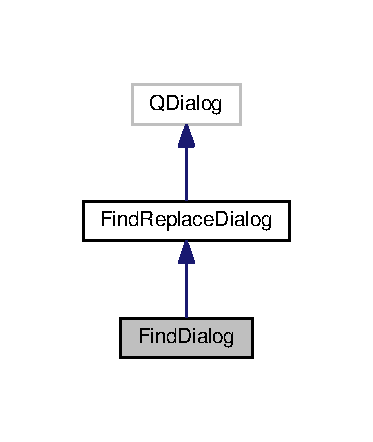
\includegraphics[width=179pt]{classFindDialog__inherit__graph}
\end{center}
\end{figure}


Collaboration diagram for Find\+Dialog\+:\nopagebreak
\begin{figure}[H]
\begin{center}
\leavevmode
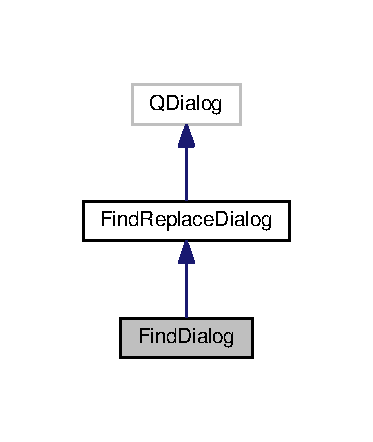
\includegraphics[width=179pt]{classFindDialog__coll__graph}
\end{center}
\end{figure}
\subsection*{Public Member Functions}
\begin{DoxyCompactItemize}
\item 
{\bfseries Find\+Dialog} (Q\+Widget $\ast$parent=nullptr)\hypertarget{classFindDialog_aa5ec2e3278ccf89baeb33dc396ea1f79}{}\label{classFindDialog_aa5ec2e3278ccf89baeb33dc396ea1f79}

\item 
virtual void {\bfseries write\+Settings} (Q\+Settings \&settings, const Q\+String \&prefix=\char`\"{}Find\+Dialog\char`\"{})\hypertarget{classFindDialog_a8d54b1576e6325b41e5989fa2cec0d26}{}\label{classFindDialog_a8d54b1576e6325b41e5989fa2cec0d26}

\item 
virtual void {\bfseries read\+Settings} (Q\+Settings \&settings, const Q\+String \&prefix=\char`\"{}Find\+Dialog\char`\"{})\hypertarget{classFindDialog_adcb3b60f3a1a4a41f7edddf7b203ba44}{}\label{classFindDialog_adcb3b60f3a1a4a41f7edddf7b203ba44}

\end{DoxyCompactItemize}
\subsection*{Additional Inherited Members}


The documentation for this class was generated from the following files\+:\begin{DoxyCompactItemize}
\item 
/home/labrat/\+Desktop/cam-\/proc/src/\+E\+R\+Database\+System/src/finddialog.\+h\item 
/home/labrat/\+Desktop/cam-\/proc/src/\+E\+R\+Database\+System/src/finddialog.\+cpp\end{DoxyCompactItemize}

\hypertarget{classFindForm}{}\section{Find\+Form Class Reference}
\label{classFindForm}\index{Find\+Form@{Find\+Form}}


Inheritance diagram for Find\+Form\+:\nopagebreak
\begin{figure}[H]
\begin{center}
\leavevmode
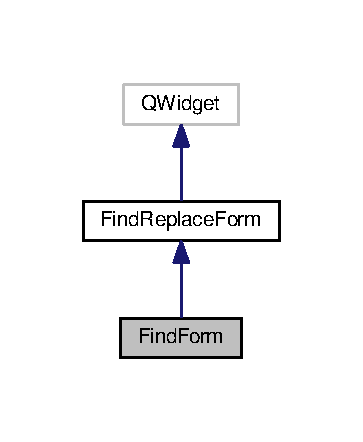
\includegraphics[width=174pt]{classFindForm__inherit__graph}
\end{center}
\end{figure}


Collaboration diagram for Find\+Form\+:\nopagebreak
\begin{figure}[H]
\begin{center}
\leavevmode
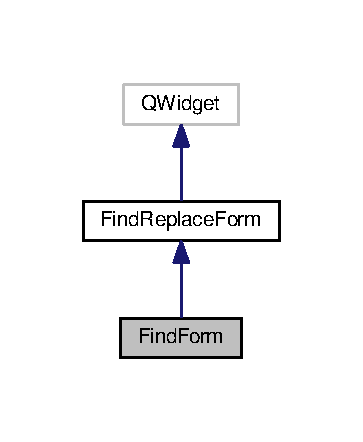
\includegraphics[width=174pt]{classFindForm__coll__graph}
\end{center}
\end{figure}
\subsection*{Public Member Functions}
\begin{DoxyCompactItemize}
\item 
{\bfseries Find\+Form} (Q\+Widget $\ast$parent=nullptr)\hypertarget{classFindForm_ae75466b4fcaff9d34d3f47eeb868e869}{}\label{classFindForm_ae75466b4fcaff9d34d3f47eeb868e869}

\item 
virtual void {\bfseries write\+Settings} (Q\+Settings \&settings, const Q\+String \&prefix=\char`\"{}Find\+Dialog\char`\"{})\hypertarget{classFindForm_a8d9f1b06d14a58d2d2a91d1d82205b4d}{}\label{classFindForm_a8d9f1b06d14a58d2d2a91d1d82205b4d}

\item 
virtual void {\bfseries read\+Settings} (Q\+Settings \&settings, const Q\+String \&prefix=\char`\"{}Find\+Dialog\char`\"{})\hypertarget{classFindForm_abfa26fe2e262103bbd9d694e748c0884}{}\label{classFindForm_abfa26fe2e262103bbd9d694e748c0884}

\end{DoxyCompactItemize}
\subsection*{Protected Member Functions}
\begin{DoxyCompactItemize}
\item 
void {\bfseries change\+Event} (Q\+Event $\ast$e)\hypertarget{classFindForm_aa1ee766531453cc558ff1a8efbfd9bf6}{}\label{classFindForm_aa1ee766531453cc558ff1a8efbfd9bf6}

\end{DoxyCompactItemize}
\subsection*{Additional Inherited Members}


The documentation for this class was generated from the following files\+:\begin{DoxyCompactItemize}
\item 
/home/labrat/\+Desktop/cam-\/proc/src/\+E\+R\+Database\+System/src/findform.\+h\item 
/home/labrat/\+Desktop/cam-\/proc/src/\+E\+R\+Database\+System/src/findform.\+cpp\end{DoxyCompactItemize}

\hypertarget{classFindReplaceDialog}{}\section{Find\+Replace\+Dialog Class Reference}
\label{classFindReplaceDialog}\index{Find\+Replace\+Dialog@{Find\+Replace\+Dialog}}


Inheritance diagram for Find\+Replace\+Dialog\+:\nopagebreak
\begin{figure}[H]
\begin{center}
\leavevmode
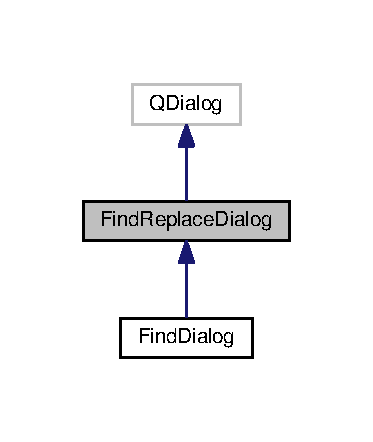
\includegraphics[width=179pt]{classFindReplaceDialog__inherit__graph}
\end{center}
\end{figure}


Collaboration diagram for Find\+Replace\+Dialog\+:\nopagebreak
\begin{figure}[H]
\begin{center}
\leavevmode
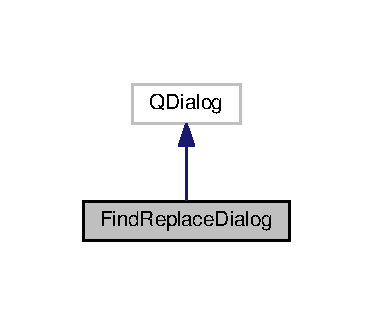
\includegraphics[width=179pt]{classFindReplaceDialog__coll__graph}
\end{center}
\end{figure}
\subsection*{Public Slots}
\begin{DoxyCompactItemize}
\item 
void {\bfseries find\+Next} ()\hypertarget{classFindReplaceDialog_ac4d4fa5eb9fdda240d855f05b5b6df68}{}\label{classFindReplaceDialog_ac4d4fa5eb9fdda240d855f05b5b6df68}

\item 
void {\bfseries find\+Prev} ()\hypertarget{classFindReplaceDialog_af48970c4a221387bc4df6b7f521af693}{}\label{classFindReplaceDialog_af48970c4a221387bc4df6b7f521af693}

\end{DoxyCompactItemize}
\subsection*{Public Member Functions}
\begin{DoxyCompactItemize}
\item 
{\bfseries Find\+Replace\+Dialog} (Q\+Widget $\ast$parent=nullptr)\hypertarget{classFindReplaceDialog_aa5a98a2773539b366980489436400357}{}\label{classFindReplaceDialog_aa5a98a2773539b366980489436400357}

\item 
void {\bfseries set\+Text\+Edit} (Q\+Text\+Edit $\ast$text\+Edit)\hypertarget{classFindReplaceDialog_a3d3cd91477be5d6529e9aa3de21958a6}{}\label{classFindReplaceDialog_a3d3cd91477be5d6529e9aa3de21958a6}

\item 
virtual void {\bfseries write\+Settings} (Q\+Settings \&settings, const Q\+String \&prefix=\char`\"{}Find\+Replace\+Dialog\char`\"{})\hypertarget{classFindReplaceDialog_ad9216d8059c559596baa5ddcbda3ec0b}{}\label{classFindReplaceDialog_ad9216d8059c559596baa5ddcbda3ec0b}

\item 
virtual void {\bfseries read\+Settings} (Q\+Settings \&settings, const Q\+String \&prefix=\char`\"{}Find\+Replace\+Dialog\char`\"{})\hypertarget{classFindReplaceDialog_a2be8b8724a5f9a7e6dff30348f94761c}{}\label{classFindReplaceDialog_a2be8b8724a5f9a7e6dff30348f94761c}

\end{DoxyCompactItemize}
\subsection*{Protected Member Functions}
\begin{DoxyCompactItemize}
\item 
void {\bfseries change\+Event} (Q\+Event $\ast$e)\hypertarget{classFindReplaceDialog_a793bc999abeaedd4262d39161f521f35}{}\label{classFindReplaceDialog_a793bc999abeaedd4262d39161f521f35}

\end{DoxyCompactItemize}
\subsection*{Protected Attributes}
\begin{DoxyCompactItemize}
\item 
Ui\+::\+Find\+Replace\+Dialog $\ast$ {\bfseries ui}\hypertarget{classFindReplaceDialog_ab2511239f2c08d5c564db4939326bfa5}{}\label{classFindReplaceDialog_ab2511239f2c08d5c564db4939326bfa5}

\end{DoxyCompactItemize}


The documentation for this class was generated from the following files\+:\begin{DoxyCompactItemize}
\item 
/home/labrat/\+Desktop/cam-\/proc/src/\+E\+R\+Database\+System/ui/findreplacedialog.\+h\item 
/home/labrat/\+Desktop/cam-\/proc/src/\+E\+R\+Database\+System/ui/findreplacedialog.\+cpp\end{DoxyCompactItemize}

\hypertarget{classFindReplaceForm}{}\section{Find\+Replace\+Form Class Reference}
\label{classFindReplaceForm}\index{Find\+Replace\+Form@{Find\+Replace\+Form}}


Inheritance diagram for Find\+Replace\+Form\+:\nopagebreak
\begin{figure}[H]
\begin{center}
\leavevmode
\includegraphics[width=174pt]{classFindReplaceForm__inherit__graph}
\end{center}
\end{figure}


Collaboration diagram for Find\+Replace\+Form\+:\nopagebreak
\begin{figure}[H]
\begin{center}
\leavevmode
\includegraphics[width=174pt]{classFindReplaceForm__coll__graph}
\end{center}
\end{figure}
\subsection*{Public Slots}
\begin{DoxyCompactItemize}
\item 
void {\bfseries find} (bool down)\hypertarget{classFindReplaceForm_af049cb8244954e17c792dc960ce544a0}{}\label{classFindReplaceForm_af049cb8244954e17c792dc960ce544a0}

\item 
void {\bfseries find} ()\hypertarget{classFindReplaceForm_ad2f83207e2b70f30680049286033915b}{}\label{classFindReplaceForm_ad2f83207e2b70f30680049286033915b}

\item 
void {\bfseries find\+Next} ()\hypertarget{classFindReplaceForm_a4aa85cfca1753dd04c1a118ac17257d9}{}\label{classFindReplaceForm_a4aa85cfca1753dd04c1a118ac17257d9}

\item 
void {\bfseries find\+Prev} ()\hypertarget{classFindReplaceForm_a98ff3bc6e591f268bb44ce02c5e70663}{}\label{classFindReplaceForm_a98ff3bc6e591f268bb44ce02c5e70663}

\item 
void {\bfseries replace} ()\hypertarget{classFindReplaceForm_abe7bcb37012970be0e5bc6e7016cb0a3}{}\label{classFindReplaceForm_abe7bcb37012970be0e5bc6e7016cb0a3}

\item 
void {\bfseries replace\+All} ()\hypertarget{classFindReplaceForm_aec41613e2aaac883f638d032d4d90d55}{}\label{classFindReplaceForm_aec41613e2aaac883f638d032d4d90d55}

\end{DoxyCompactItemize}
\subsection*{Public Member Functions}
\begin{DoxyCompactItemize}
\item 
{\bfseries Find\+Replace\+Form} (Q\+Widget $\ast$parent=nullptr)\hypertarget{classFindReplaceForm_ae873449e492183b9c3ddee64b288e4e6}{}\label{classFindReplaceForm_ae873449e492183b9c3ddee64b288e4e6}

\item 
void {\bfseries set\+Text\+Edit} (Q\+Text\+Edit $\ast$text\+Edit\+\_\+)\hypertarget{classFindReplaceForm_ad621f91f15f0902a050c67e66c839d6f}{}\label{classFindReplaceForm_ad621f91f15f0902a050c67e66c839d6f}

\item 
void {\bfseries hide\+Replace\+Widgets} ()\hypertarget{classFindReplaceForm_acd7c42b7ef674ca414d0e47158fdad31}{}\label{classFindReplaceForm_acd7c42b7ef674ca414d0e47158fdad31}

\item 
virtual void {\bfseries write\+Settings} (Q\+Settings \&settings, const Q\+String \&prefix=\char`\"{}Find\+Replace\+Dialog\char`\"{})\hypertarget{classFindReplaceForm_a8746401be4fbab54b6019a76e05e7b43}{}\label{classFindReplaceForm_a8746401be4fbab54b6019a76e05e7b43}

\item 
virtual void {\bfseries read\+Settings} (Q\+Settings \&settings, const Q\+String \&prefix=\char`\"{}Find\+Replace\+Dialog\char`\"{})\hypertarget{classFindReplaceForm_a87e0f16b427e570ede2a219b16300c2a}{}\label{classFindReplaceForm_a87e0f16b427e570ede2a219b16300c2a}

\end{DoxyCompactItemize}
\subsection*{Protected Slots}
\begin{DoxyCompactItemize}
\item 
void {\bfseries text\+To\+Find\+Changed} ()\hypertarget{classFindReplaceForm_a0fd7fa8014c190857e5c3be4392fc96a}{}\label{classFindReplaceForm_a0fd7fa8014c190857e5c3be4392fc96a}

\item 
void {\bfseries validate\+Reg\+Exp} (const Q\+String \&text)\hypertarget{classFindReplaceForm_a2867ac36c3f8c9accb7f0c010ee74522}{}\label{classFindReplaceForm_a2867ac36c3f8c9accb7f0c010ee74522}

\item 
void {\bfseries regexp\+Selected} (bool sel)\hypertarget{classFindReplaceForm_acbde49b9b3e2efd6940f8d2e16b9172c}{}\label{classFindReplaceForm_acbde49b9b3e2efd6940f8d2e16b9172c}

\end{DoxyCompactItemize}
\subsection*{Protected Member Functions}
\begin{DoxyCompactItemize}
\item 
void {\bfseries change\+Event} (Q\+Event $\ast$e)\hypertarget{classFindReplaceForm_a67f57e1f82d146cd0019cd64aa147e4b}{}\label{classFindReplaceForm_a67f57e1f82d146cd0019cd64aa147e4b}

\item 
void {\bfseries show\+Error} (const Q\+String \&error)\hypertarget{classFindReplaceForm_a49bcdfa2193f0fb5fa8ccbbf1875d893}{}\label{classFindReplaceForm_a49bcdfa2193f0fb5fa8ccbbf1875d893}

\item 
void {\bfseries show\+Message} (const Q\+String \&message)\hypertarget{classFindReplaceForm_a39929b108e4e85a9d64366777e9fde22}{}\label{classFindReplaceForm_a39929b108e4e85a9d64366777e9fde22}

\end{DoxyCompactItemize}
\subsection*{Protected Attributes}
\begin{DoxyCompactItemize}
\item 
Ui\+::\+Find\+Replace\+Form $\ast$ {\bfseries ui}\hypertarget{classFindReplaceForm_a9bf9e9096feff863dcd6c2a989e07d2c}{}\label{classFindReplaceForm_a9bf9e9096feff863dcd6c2a989e07d2c}

\item 
Q\+Text\+Cursor {\bfseries text\+Cursor}\hypertarget{classFindReplaceForm_acbbc970423e9e4dfcee99d53e02d8eb2}{}\label{classFindReplaceForm_acbbc970423e9e4dfcee99d53e02d8eb2}

\item 
Q\+Text\+Edit $\ast$ {\bfseries text\+Edit}\hypertarget{classFindReplaceForm_a6ddb6c32035bcafdd085c457c1ac125c}{}\label{classFindReplaceForm_a6ddb6c32035bcafdd085c457c1ac125c}

\end{DoxyCompactItemize}


The documentation for this class was generated from the following files\+:\begin{DoxyCompactItemize}
\item 
/home/labrat/\+Desktop/cam-\/proc/src/\+E\+R\+Database\+System/ui/findreplaceform.\+h\item 
/home/labrat/\+Desktop/cam-\/proc/src/\+E\+R\+Database\+System/ui/findreplaceform.\+cpp\end{DoxyCompactItemize}

\hypertarget{classfirstNestedTable}{}\section{first\+Nested\+Table Class Reference}
\label{classfirstNestedTable}\index{first\+Nested\+Table@{first\+Nested\+Table}}


Inheritance diagram for first\+Nested\+Table\+:\nopagebreak
\begin{figure}[H]
\begin{center}
\leavevmode
\includegraphics[width=169pt]{classfirstNestedTable__inherit__graph}
\end{center}
\end{figure}


Collaboration diagram for first\+Nested\+Table\+:\nopagebreak
\begin{figure}[H]
\begin{center}
\leavevmode
\includegraphics[width=169pt]{classfirstNestedTable__coll__graph}
\end{center}
\end{figure}
\subsection*{Public Types}
\begin{DoxyCompactItemize}
\item 
enum {\bfseries Opening} \{ {\bfseries O\+P\+E\+N\+I\+NG}, 
{\bfseries S\+A\+V\+I\+NG}
 \}\hypertarget{classfirstNestedTable_afb790c3fd0e9a06e01ba62e50f04039c}{}\label{classfirstNestedTable_afb790c3fd0e9a06e01ba62e50f04039c}

\end{DoxyCompactItemize}
\subsection*{Public Member Functions}
\begin{DoxyCompactItemize}
\item 
{\bfseries first\+Nested\+Table} (Q\+Widget $\ast$parent=nullptr)\hypertarget{classfirstNestedTable_a8eeeb1d32c3e24a6c028c4dd374df3b6}{}\label{classfirstNestedTable_a8eeeb1d32c3e24a6c028c4dd374df3b6}

\item 
void {\bfseries set\+Name} (Q\+String table)\hypertarget{classfirstNestedTable_adcd2612cb8f46d9c223b7d89f08286e6}{}\label{classfirstNestedTable_adcd2612cb8f46d9c223b7d89f08286e6}

\item 
void {\bfseries update\+Images} ()\hypertarget{classfirstNestedTable_ac1625ffee7e65e0b168b642326353ad2}{}\label{classfirstNestedTable_ac1625ffee7e65e0b168b642326353ad2}

\end{DoxyCompactItemize}


The documentation for this class was generated from the following files\+:\begin{DoxyCompactItemize}
\item 
/home/labrat/\+Desktop/cam-\/proc/src/\+E\+R\+Database\+System/ui/firstnestedtable.\+h\item 
/home/labrat/\+Desktop/cam-\/proc/src/\+E\+R\+Database\+System/ui/firstnestedtable.\+cpp\end{DoxyCompactItemize}

\hypertarget{classfirstTableXmlExcelCSV}{}\section{first\+Table\+Xml\+Excel\+C\+SV Class Reference}
\label{classfirstTableXmlExcelCSV}\index{first\+Table\+Xml\+Excel\+C\+SV@{first\+Table\+Xml\+Excel\+C\+SV}}


Inheritance diagram for first\+Table\+Xml\+Excel\+C\+SV\+:\nopagebreak
\begin{figure}[H]
\begin{center}
\leavevmode
\includegraphics[width=200pt]{classfirstTableXmlExcelCSV__inherit__graph}
\end{center}
\end{figure}


Collaboration diagram for first\+Table\+Xml\+Excel\+C\+SV\+:\nopagebreak
\begin{figure}[H]
\begin{center}
\leavevmode
\includegraphics[width=200pt]{classfirstTableXmlExcelCSV__coll__graph}
\end{center}
\end{figure}
\subsection*{Public Member Functions}
\begin{DoxyCompactItemize}
\item 
{\bfseries first\+Table\+Xml\+Excel\+C\+SV} (Q\+Widget $\ast$parent=nullptr)\hypertarget{classfirstTableXmlExcelCSV_ab444fbb8fb7e7433889875f0db199277}{}\label{classfirstTableXmlExcelCSV_ab444fbb8fb7e7433889875f0db199277}

\item 
void \hyperlink{classfirstTableXmlExcelCSV_a301b1fa4836f679d59b62a4785d69f32}{set\+Model} (Q\+String table, Q\+Abstract\+Item\+Model $\ast$model)
\end{DoxyCompactItemize}


\subsection{Member Function Documentation}
\index{first\+Table\+Xml\+Excel\+C\+SV@{first\+Table\+Xml\+Excel\+C\+SV}!set\+Model@{set\+Model}}
\index{set\+Model@{set\+Model}!first\+Table\+Xml\+Excel\+C\+SV@{first\+Table\+Xml\+Excel\+C\+SV}}
\subsubsection[{\texorpdfstring{set\+Model(\+Q\+String table, Q\+Abstract\+Item\+Model $\ast$model)}{setModel(QString table, QAbstractItemModel *model)}}]{\setlength{\rightskip}{0pt plus 5cm}void first\+Table\+Xml\+Excel\+C\+S\+V\+::set\+Model (
\begin{DoxyParamCaption}
\item[{Q\+String}]{table, }
\item[{Q\+Abstract\+Item\+Model $\ast$}]{model}
\end{DoxyParamCaption}
)}\hypertarget{classfirstTableXmlExcelCSV_a301b1fa4836f679d59b62a4785d69f32}{}\label{classfirstTableXmlExcelCSV_a301b1fa4836f679d59b62a4785d69f32}
call for struct 

The documentation for this class was generated from the following files\+:\begin{DoxyCompactItemize}
\item 
/home/labrat/\+Desktop/cam-\/proc/src/\+E\+R\+Database\+System/ui/firsttablexmlexcelcsv.\+h\item 
/home/labrat/\+Desktop/cam-\/proc/src/\+E\+R\+Database\+System/ui/firsttablexmlexcelcsv.\+cpp\end{DoxyCompactItemize}

\hypertarget{classFlannMatcher}{}\section{Flann\+Matcher Class Reference}
\label{classFlannMatcher}\index{Flann\+Matcher@{Flann\+Matcher}}


Inheritance diagram for Flann\+Matcher\+:\nopagebreak
\begin{figure}[H]
\begin{center}
\leavevmode
\includegraphics[width=169pt]{classFlannMatcher__inherit__graph}
\end{center}
\end{figure}


Collaboration diagram for Flann\+Matcher\+:\nopagebreak
\begin{figure}[H]
\begin{center}
\leavevmode
\includegraphics[width=169pt]{classFlannMatcher__coll__graph}
\end{center}
\end{figure}
\subsection*{Public Member Functions}
\begin{DoxyCompactItemize}
\item 
\hyperlink{classImage}{Image} {\bfseries match\+Preview} (unsigned int i)\hypertarget{classFlannMatcher_a37b2e9dbfff55df6acea295e333ae33d}{}\label{classFlannMatcher_a37b2e9dbfff55df6acea295e333ae33d}

\item 
std\+::vector$<$ cv\+::\+D\+Match $>$ {\bfseries find\+Maches} (cv\+::\+Mat descA, cv\+::\+Mat descB)\hypertarget{classFlannMatcher_ac7540ea9a30c3b87d14d39a5ba130266}{}\label{classFlannMatcher_ac7540ea9a30c3b87d14d39a5ba130266}

\item 
std\+::vector$<$ cv\+::\+D\+Match $>$ {\bfseries find\+Maches} (unsigned int i)\hypertarget{classFlannMatcher_a0d1ed99600a58b8da8a9dabf8fb22eab}{}\label{classFlannMatcher_a0d1ed99600a58b8da8a9dabf8fb22eab}

\item 
void {\bfseries find\+Features} ()\hypertarget{classFlannMatcher_aa9610e702c5d0ed9e1565ad0e514afd1}{}\label{classFlannMatcher_aa9610e702c5d0ed9e1565ad0e514afd1}

\item 
void {\bfseries set\+Tolerance} (float tolerance)\hypertarget{classFlannMatcher_a42ddfde49e5cbda63ab8d5efbd1b8600}{}\label{classFlannMatcher_a42ddfde49e5cbda63ab8d5efbd1b8600}

\end{DoxyCompactItemize}
\subsection*{Protected Member Functions}
\begin{DoxyCompactItemize}
\item 
void {\bfseries run\+Operations} ()\hypertarget{classFlannMatcher_a67308488c12bbd3408b4aca3016e66a1}{}\label{classFlannMatcher_a67308488c12bbd3408b4aca3016e66a1}

\end{DoxyCompactItemize}
\subsection*{Protected Attributes}
\begin{DoxyCompactItemize}
\item 
cv\+::\+Flann\+Based\+Matcher {\bfseries \+\_\+matcher}\hypertarget{classFlannMatcher_a187d368edc6a237718516f3010cc7bf9}{}\label{classFlannMatcher_a187d368edc6a237718516f3010cc7bf9}

\item 
float {\bfseries \+\_\+tolerance}\hypertarget{classFlannMatcher_a60a1d4356fec7c52f888a17729d11270}{}\label{classFlannMatcher_a60a1d4356fec7c52f888a17729d11270}

\end{DoxyCompactItemize}


The documentation for this class was generated from the following files\+:\begin{DoxyCompactItemize}
\item 
/home/labrat/\+Desktop/cam-\/proc/src/feature\+Matcher/flannmatcher.\+h\item 
/home/labrat/\+Desktop/cam-\/proc/src/feature\+Matcher/flannmatcher.\+cpp\end{DoxyCompactItemize}

\hypertarget{classFlannWidget}{}\section{Flann\+Widget Class Reference}
\label{classFlannWidget}\index{Flann\+Widget@{Flann\+Widget}}


Inheritance diagram for Flann\+Widget\+:\nopagebreak
\begin{figure}[H]
\begin{center}
\leavevmode
\includegraphics[width=157pt]{classFlannWidget__inherit__graph}
\end{center}
\end{figure}


Collaboration diagram for Flann\+Widget\+:\nopagebreak
\begin{figure}[H]
\begin{center}
\leavevmode
\includegraphics[width=157pt]{classFlannWidget__coll__graph}
\end{center}
\end{figure}
\subsection*{Public Member Functions}
\begin{DoxyCompactItemize}
\item 
{\bfseries Flann\+Widget} (\hyperlink{classStereoToolbar}{Stereo\+Toolbar} $\ast$parent=0)\hypertarget{classFlannWidget_ac76c1cd3d8ad93c983845722064ff428}{}\label{classFlannWidget_ac76c1cd3d8ad93c983845722064ff428}

\item 
\hyperlink{classFlannMatcher}{Flann\+Matcher} \& {\bfseries get\+Processor} ()\hypertarget{classFlannWidget_ae4043b465aed916fa0464e179fa41843}{}\label{classFlannWidget_ae4043b465aed916fa0464e179fa41843}

\item 
void {\bfseries update} ()\hypertarget{classFlannWidget_a6e48067006112ce8b317552833a6cbd5}{}\label{classFlannWidget_a6e48067006112ce8b317552833a6cbd5}

\end{DoxyCompactItemize}


The documentation for this class was generated from the following files\+:\begin{DoxyCompactItemize}
\item 
/home/labrat/\+Desktop/cam-\/proc/src/feature\+Matcher/flannwidget.\+h\item 
/home/labrat/\+Desktop/cam-\/proc/src/feature\+Matcher/flannwidget.\+cpp\end{DoxyCompactItemize}

\hypertarget{classgreyifyer}{}\section{greyifyer Class Reference}
\label{classgreyifyer}\index{greyifyer@{greyifyer}}
\subsection*{Public Member Functions}
\begin{DoxyCompactItemize}
\item 
void {\bfseries set\+Image\+Dir} (std\+::string path)\hypertarget{classgreyifyer_a65bb66356ffbb4ab2d353b5b8570e4aa}{}\label{classgreyifyer_a65bb66356ffbb4ab2d353b5b8570e4aa}

\item 
std\+::shared\+\_\+ptr$<$ \hyperlink{classImageList}{Image\+List}$<$ \hyperlink{classImage}{Image} $>$ $>$ {\bfseries get\+Image\+List} ()\hypertarget{classgreyifyer_a2e649c47dee46bbfab3657775b1c802e}{}\label{classgreyifyer_a2e649c47dee46bbfab3657775b1c802e}

\item 
void {\bfseries convert\+To\+Grey} ()\hypertarget{classgreyifyer_a8e9e7e3087f18385676263068115916f}{}\label{classgreyifyer_a8e9e7e3087f18385676263068115916f}

\end{DoxyCompactItemize}


The documentation for this class was generated from the following files\+:\begin{DoxyCompactItemize}
\item 
/home/labrat/\+Desktop/cam-\/proc/src/bio\+Database/src/greyifyer.\+h\item 
/home/labrat/\+Desktop/cam-\/proc/src/bio\+Database/src/greyifyer.\+cpp\end{DoxyCompactItemize}

\hypertarget{classGreyifyer}{}\section{Greyifyer Class Reference}
\label{classGreyifyer}\index{Greyifyer@{Greyifyer}}
\subsection*{Public Member Functions}
\begin{DoxyCompactItemize}
\item 
void {\bfseries set\+Image\+Dir} (std\+::string path)\hypertarget{classGreyifyer_a3ecc65a618fe1f7ed2788ee9f2ba5c66}{}\label{classGreyifyer_a3ecc65a618fe1f7ed2788ee9f2ba5c66}

\item 
std\+::shared\+\_\+ptr$<$ \hyperlink{classImageList}{Image\+List}$<$ \hyperlink{classImage}{Image} $>$ $>$ {\bfseries get\+Image\+List} ()\hypertarget{classGreyifyer_ad024a91d058b89e314f5c5a4118bfdce}{}\label{classGreyifyer_ad024a91d058b89e314f5c5a4118bfdce}

\item 
void {\bfseries convert\+To\+Grey} ()\hypertarget{classGreyifyer_a58554aa7ec682f2c335de41392e8f0b4}{}\label{classGreyifyer_a58554aa7ec682f2c335de41392e8f0b4}

\end{DoxyCompactItemize}


The documentation for this class was generated from the following files\+:\begin{DoxyCompactItemize}
\item 
/home/labrat/\+Desktop/cam-\/proc/src/hello\+Lib\+Cam\+U\+I/src/greyifyer.\+h\item 
/home/labrat/\+Desktop/cam-\/proc/src/hello\+Lib\+Cam\+U\+I/src/greyifyer.\+cpp\end{DoxyCompactItemize}

\hypertarget{classHistEqualizer}{}\section{Hist\+Equalizer Class Reference}
\label{classHistEqualizer}\index{Hist\+Equalizer@{Hist\+Equalizer}}


Inheritance diagram for Hist\+Equalizer\+:\nopagebreak
\begin{figure}[H]
\begin{center}
\leavevmode
\includegraphics[width=168pt]{classHistEqualizer__inherit__graph}
\end{center}
\end{figure}


Collaboration diagram for Hist\+Equalizer\+:\nopagebreak
\begin{figure}[H]
\begin{center}
\leavevmode
\includegraphics[width=168pt]{classHistEqualizer__coll__graph}
\end{center}
\end{figure}
\subsection*{Public Member Functions}
\begin{DoxyCompactItemize}
\item 
void {\bfseries eqalize} (\hyperlink{classImage}{Image} \&img)\hypertarget{classHistEqualizer_ad26e0836fde98f6152bfe060a45fd6d4}{}\label{classHistEqualizer_ad26e0836fde98f6152bfe060a45fd6d4}

\end{DoxyCompactItemize}
\subsection*{Public Attributes}
\begin{DoxyCompactItemize}
\item 
int {\bfseries chan}\hypertarget{classHistEqualizer_a734bad8d5c068aa61c4be3234059c4fb}{}\label{classHistEqualizer_a734bad8d5c068aa61c4be3234059c4fb}

\item 
std\+::vector$<$ int $>$ {\bfseries upper}\hypertarget{classHistEqualizer_a278935336e7f82453ce167c9c678e183}{}\label{classHistEqualizer_a278935336e7f82453ce167c9c678e183}

\item 
std\+::vector$<$ int $>$ {\bfseries lower}\hypertarget{classHistEqualizer_a5a2d6be17250463714a57d47775b2379}{}\label{classHistEqualizer_a5a2d6be17250463714a57d47775b2379}

\end{DoxyCompactItemize}
\subsection*{Protected Member Functions}
\begin{DoxyCompactItemize}
\item 
void {\bfseries run\+Operations} ()\hypertarget{classHistEqualizer_a9364b0f5e615b7623a029400b710c06a}{}\label{classHistEqualizer_a9364b0f5e615b7623a029400b710c06a}

\end{DoxyCompactItemize}
\subsection*{Additional Inherited Members}


The documentation for this class was generated from the following files\+:\begin{DoxyCompactItemize}
\item 
/home/labrat/\+Desktop/cam-\/proc/src/color\+Corrector/src/histequalizer.\+h\item 
/home/labrat/\+Desktop/cam-\/proc/src/color\+Corrector/src/histequalizer.\+cpp\end{DoxyCompactItemize}

\hypertarget{classHistEqWidget}{}\section{Hist\+Eq\+Widget Class Reference}
\label{classHistEqWidget}\index{Hist\+Eq\+Widget@{Hist\+Eq\+Widget}}


Inheritance diagram for Hist\+Eq\+Widget\+:\nopagebreak
\begin{figure}[H]
\begin{center}
\leavevmode
\includegraphics[width=166pt]{classHistEqWidget__inherit__graph}
\end{center}
\end{figure}


Collaboration diagram for Hist\+Eq\+Widget\+:\nopagebreak
\begin{figure}[H]
\begin{center}
\leavevmode
\includegraphics[width=166pt]{classHistEqWidget__coll__graph}
\end{center}
\end{figure}
\subsection*{Public Member Functions}
\begin{DoxyCompactItemize}
\item 
{\bfseries Hist\+Eq\+Widget} (\hyperlink{classAbstractToolbar}{Abstract\+Toolbar} $\ast$parent=0)\hypertarget{classHistEqWidget_ae317f920e5f91a03416bba6c49f0c007}{}\label{classHistEqWidget_ae317f920e5f91a03416bba6c49f0c007}

\item 
\hyperlink{classHistEqualizer}{Hist\+Equalizer} \& {\bfseries get\+Processor} ()\hypertarget{classHistEqWidget_a6bfdd913cab30f0e38fdd31bd2c236df}{}\label{classHistEqWidget_a6bfdd913cab30f0e38fdd31bd2c236df}

\item 
void {\bfseries update} ()\hypertarget{classHistEqWidget_a4e638f807b015ff30d7f861093cda2b3}{}\label{classHistEqWidget_a4e638f807b015ff30d7f861093cda2b3}

\item 
void {\bfseries generate\+Preview} ()\hypertarget{classHistEqWidget_a3ca663bde2818e3249344e77c9517971}{}\label{classHistEqWidget_a3ca663bde2818e3249344e77c9517971}

\item 
std\+::string {\bfseries get\+Name} ()\hypertarget{classHistEqWidget_ae7a2b0b3ff48971b844b637ee9a1e7e9}{}\label{classHistEqWidget_ae7a2b0b3ff48971b844b637ee9a1e7e9}

\end{DoxyCompactItemize}


The documentation for this class was generated from the following files\+:\begin{DoxyCompactItemize}
\item 
/home/labrat/\+Desktop/cam-\/proc/src/color\+Corrector/ui/histeqwidget.\+h\item 
/home/labrat/\+Desktop/cam-\/proc/src/color\+Corrector/ui/histeqwidget.\+cpp\end{DoxyCompactItemize}

\hypertarget{classImage}{}\section{Image Class Reference}
\label{classImage}\index{Image@{Image}}


Inheritance diagram for Image\+:\nopagebreak
\begin{figure}[H]
\begin{center}
\leavevmode
\includegraphics[width=256pt]{classImage__inherit__graph}
\end{center}
\end{figure}


Collaboration diagram for Image\+:\nopagebreak
\begin{figure}[H]
\begin{center}
\leavevmode
\includegraphics[width=262pt]{classImage__coll__graph}
\end{center}
\end{figure}
\subsection*{Classes}
\begin{DoxyCompactItemize}
\item 
struct \hyperlink{structImage_1_1TiffTag__t}{Tiff\+Tag\+\_\+t}
\begin{DoxyCompactList}\small\item\em the values pulled from the proscillica tifftags \end{DoxyCompactList}\end{DoxyCompactItemize}
\subsection*{Public Member Functions}
\begin{DoxyCompactItemize}
\item 
void \hyperlink{classImage_ab5a21f84f8a2acda7a63567f1078e35c}{initialize} (Color\+Space cs)
\begin{DoxyCompactList}\small\item\em initialize an image with a specified Color\+Space \end{DoxyCompactList}\item 
void {\bfseries set\+Read\+Only} (bool x)\hypertarget{classImage_a091620a35574d2c404ae6a8946dae33e}{}\label{classImage_a091620a35574d2c404ae6a8946dae33e}

\item 
bool \hyperlink{classImage_a87e5728d527b4e28f8696a4f266f07e7}{set\+Bitmap} (cv\+::\+Mat bmp)
\begin{DoxyCompactList}\small\item\em Set the bitmap of the \hyperlink{classImage}{Image}. \end{DoxyCompactList}\item 
bool \hyperlink{classImage_ac0cc82352caee90c6faa9401663e16fd}{read\+From\+File} (std\+::string f\+Name, Color\+Space cs=B\+GR)
\begin{DoxyCompactList}\small\item\em Load an image from a file on disk. \end{DoxyCompactList}\item 
bool \hyperlink{classImage_aa2f3974b50f53aecfca04077b5ccadf6}{read\+From\+File} (boost\+::filesystem\+::path file\+Path, Color\+Space cs=B\+GR)
\begin{DoxyCompactList}\small\item\em Load an image from a file on disk. \end{DoxyCompactList}\item 
cv\+::\+Mat \& \hyperlink{classImage_a75c5976f165be3d79b745d3d0a297662}{get\+Bitmap} ()
\begin{DoxyCompactList}\small\item\em set the parameters for the image so that I can find it in the DB \end{DoxyCompactList}\item 
cv\+::\+Mat {\bfseries get8\+Bitmap} ()\hypertarget{classImage_a4a6e8b26ab1004190896faf55f0f7616}{}\label{classImage_a4a6e8b26ab1004190896faf55f0f7616}

\item 
cv\+::\+Mat {\bfseries get16\+Bitmap} ()\hypertarget{classImage_aa8aebc050b89bbaae627c12880b6088d}{}\label{classImage_aa8aebc050b89bbaae627c12880b6088d}

\item 
bool \hyperlink{classImage_a1a393960f7402515428bd982c32f59af}{load} ()
\begin{DoxyCompactList}\small\item\em loads stored filename into memory. Will N\+OT reload if image was already loaded \end{DoxyCompactList}\item 
bool \hyperlink{classImage_a37b7fbb0e61bf13f86557f507478ac38}{load\+From\+DB} ()
\begin{DoxyCompactList}\small\item\em populates the \+\_\+bitmap \end{DoxyCompactList}\item 
bool \hyperlink{classImage_a23899e8362a6755cc51f46fd490881ba}{load\+From\+File} ()
\item 
void \hyperlink{classImage_a4197ac415ed55494d21d9fae506ee806}{unload} ()
\begin{DoxyCompactList}\small\item\em Removes an image from R\+AM and stores (caches) it to the \+\_\+save\+Path. \end{DoxyCompactList}\item 
void \hyperlink{classImage_a643d9f46961e8372b6a573246aad66d1}{save} ()
\begin{DoxyCompactList}\small\item\em save an image to the save path set by Image\+::set\+Save\+Path \end{DoxyCompactList}\item 
void \hyperlink{classImage_a8d3bca1c0c20e4a8740b883f3f61bd87}{save\+To\+DB} ()
\item 
void \hyperlink{classImage_a94e5fcd0ba589d8187393d230d15b83d}{save\+To\+File} ()
\item 
boost\+::filesystem\+::path {\bfseries get\+Load\+Path} ()\hypertarget{classImage_a6269eaa2758e10a6644e68bc878fdec6}{}\label{classImage_a6269eaa2758e10a6644e68bc878fdec6}

\item 
boost\+::filesystem\+::path {\bfseries get\+Save\+Path} ()\hypertarget{classImage_ac6f982ea176c5d1fd95cfded780bb8de}{}\label{classImage_ac6f982ea176c5d1fd95cfded780bb8de}

\item 
void {\bfseries set\+Save\+Path} (boost\+::filesystem\+::path p)\hypertarget{classImage_ae7533f776abe2e1b4e6681985ba66aab}{}\label{classImage_ae7533f776abe2e1b4e6681985ba66aab}

\item 
void {\bfseries set\+Save\+D\+B\+Param} ()\hypertarget{classImage_a55ff7e2ed3f552f49f9ea139e4545718}{}\label{classImage_a55ff7e2ed3f552f49f9ea139e4545718}

\item 
std\+::string {\bfseries get\+Name} () const \hypertarget{classImage_acdd2b0d19aa5f00e1177e700db2bea5b}{}\label{classImage_acdd2b0d19aa5f00e1177e700db2bea5b}

\item 
unsigned long {\bfseries get\+U\+Time} ()\hypertarget{classImage_a1cb942960098498f91b180909913c10b}{}\label{classImage_a1cb942960098498f91b180909913c10b}

\item 
void {\bfseries set\+Name} (std\+::string str)\hypertarget{classImage_aa4e028c7e168f66d705b6e1a9072ee1d}{}\label{classImage_aa4e028c7e168f66d705b6e1a9072ee1d}

\item 
cv\+::\+Mat \hyperlink{classImage_ab5320afddf5e1f2f91de8b55d4c34f4f}{generate\+Hist} ()
\begin{DoxyCompactList}\small\item\em This function returns a Histogram inf the form of a cv\+::\+Mat. \end{DoxyCompactList}\item 
void {\bfseries display\+Hist} (std\+::string window\+Name)\hypertarget{classImage_ac90012db4bf46088777b9e03a9c20700}{}\label{classImage_ac90012db4bf46088777b9e03a9c20700}

\item 
std\+::vector$<$ std\+::string $>$ \& {\bfseries get\+Channels} ()\hypertarget{classImage_a52c5c706f2a5b87271b1d817b61f3b59}{}\label{classImage_a52c5c706f2a5b87271b1d817b61f3b59}

\item 
\hyperlink{classImage}{Image} {\bfseries get\+Copy} ()\hypertarget{classImage_a03bf7a24f3a8c010430384dde4e46304}{}\label{classImage_a03bf7a24f3a8c010430384dde4e46304}

\item 
bool \hyperlink{classImage_a7a3bf833c8e740d483f46eff90c90889}{is\+Loaded} ()
\begin{DoxyCompactList}\small\item\em a simple check to determine if the data is loaded \end{DoxyCompactList}\item 
void {\bfseries to8\+Bit} ()\hypertarget{classImage_abb27cf7805e76d571e8353b77c8f02a4}{}\label{classImage_abb27cf7805e76d571e8353b77c8f02a4}

\item 
void {\bfseries to\+Grey} ()\hypertarget{classImage_a708cddc0be49dc2a2fb5baeb8de7243d}{}\label{classImage_a708cddc0be49dc2a2fb5baeb8de7243d}

\item 
void {\bfseries to\+B\+GR} ()\hypertarget{classImage_a45ab66f3333a4269d96b8e4737c4b3dd}{}\label{classImage_a45ab66f3333a4269d96b8e4737c4b3dd}

\item 
void {\bfseries to\+R\+GB} ()\hypertarget{classImage_a36d5d12820681cc556f6424dace28592}{}\label{classImage_a36d5d12820681cc556f6424dace28592}

\item 
void {\bfseries to\+H\+SV} ()\hypertarget{classImage_ae0bbaf7bf9b4622ca7ee52912d9f47f2}{}\label{classImage_ae0bbaf7bf9b4622ca7ee52912d9f47f2}

\item 
void {\bfseries to8\+Bit\+Grey} ()\hypertarget{classImage_aede7554ad24dfc8d69e491d35a6d77d8}{}\label{classImage_aede7554ad24dfc8d69e491d35a6d77d8}

\item 
Color\+Space \& {\bfseries get\+Color\+Space} ()\hypertarget{classImage_a70d42eb45b552b08b2d4e91620a43479}{}\label{classImage_a70d42eb45b552b08b2d4e91620a43479}

\item 
{\bfseries Image} (const \hyperlink{classImage}{Image} \&other)\hypertarget{classImage_a5a3bc57bd7ba53f9ae55b1963b9ba0a1}{}\label{classImage_a5a3bc57bd7ba53f9ae55b1963b9ba0a1}

\item 
\hyperlink{classImage}{Image} \& {\bfseries operator=} (const \hyperlink{classImage}{Image} \&other)\hypertarget{classImage_a3037a583d17594b1835d9b6b8d09875c}{}\label{classImage_a3037a583d17594b1835d9b6b8d09875c}

\item 
bool {\bfseries operator$<$} (\hyperlink{classImage}{Image} const \&rhs) const \hypertarget{classImage_a084be7e5413180208d54077f17bf124f}{}\label{classImage_a084be7e5413180208d54077f17bf124f}

\item 
\hyperlink{structImage_1_1TiffTag__t}{Tiff\+Tag\+\_\+t} {\bfseries get\+Tiff\+Tag} ()\hypertarget{classImage_ac406cd1b38c6cadd4f93b8b40b64e258}{}\label{classImage_ac406cd1b38c6cadd4f93b8b40b64e258}

\item 
time\+\_\+t {\bfseries time} ()\hypertarget{classImage_a30253abde880671f30418829d8fba213}{}\label{classImage_a30253abde880671f30418829d8fba213}

\item 
long double {\bfseries img\+Float\+Time} ()\hypertarget{classImage_a26cd3cc2ba62c392421258788a2359e0}{}\label{classImage_a26cd3cc2ba62c392421258788a2359e0}

\item 
virtual void {\bfseries on\+File\+Set} ()\hypertarget{classImage_aac15594555d7479747ae0730444f89f2}{}\label{classImage_aac15594555d7479747ae0730444f89f2}

\item 
virtual void {\bfseries write\+DB} (std\+::string table, Q\+Sql\+Database m\+Database)\hypertarget{classImage_a2bc415e23666a6f85557cd270bcacae0}{}\label{classImage_a2bc415e23666a6f85557cd270bcacae0}

\item 
virtual Q\+String\+List {\bfseries read\+D\+B\+Tables} (Q\+Sql\+Database m\+Database)\hypertarget{classImage_a208498504b7aef66f5671596c3b99601}{}\label{classImage_a208498504b7aef66f5671596c3b99601}

\item 
virtual std\+::string {\bfseries get\+D\+B\+Table\+Description} (Q\+Sql\+Database m\+Database)\hypertarget{classImage_a4de05a161fa65cefbdc9a50f406c45a7}{}\label{classImage_a4de05a161fa65cefbdc9a50f406c45a7}

\end{DoxyCompactItemize}
\subsection*{Protected Member Functions}
\begin{DoxyCompactItemize}
\item 
void {\bfseries parse\+Time} ()\hypertarget{classImage_adf09c3545b003199640276db553efc30}{}\label{classImage_adf09c3545b003199640276db553efc30}

\item 
void {\bfseries read\+Tiff\+Tags} ()\hypertarget{classImage_a8b17b83fee9978e7595b491a53a50445}{}\label{classImage_a8b17b83fee9978e7595b491a53a50445}

\end{DoxyCompactItemize}
\subsection*{Protected Attributes}
\begin{DoxyCompactItemize}
\item 
std\+::mutex {\bfseries \+\_\+child\+Mutex}\hypertarget{classImage_a64bb7abc523a4788f67325e9546f6930}{}\label{classImage_a64bb7abc523a4788f67325e9546f6930}

\item 
std\+::mutex {\bfseries mtx}\hypertarget{classImage_a395fed1c28872b35071d1c20bd7e8d4a}{}\label{classImage_a395fed1c28872b35071d1c20bd7e8d4a}

\item 
Color\+Space {\bfseries \+\_\+color\+Space}\hypertarget{classImage_a7e53861a6bf28cc17f50b455b2e12870}{}\label{classImage_a7e53861a6bf28cc17f50b455b2e12870}

\item 
std\+::vector$<$ std\+::string $>$ {\bfseries \+\_\+channels}\hypertarget{classImage_ae124805d09fdb8a4c5949d26be8b5665}{}\label{classImage_ae124805d09fdb8a4c5949d26be8b5665}

\item 
cv\+::\+Mat {\bfseries \+\_\+bitmap}\hypertarget{classImage_aa6dccdccfa626658a905158033b94350}{}\label{classImage_aa6dccdccfa626658a905158033b94350}

\item 
bool {\bfseries \+\_\+pre\+Load\+On}\hypertarget{classImage_a34e92624409041b70f4f7e8178772daa}{}\label{classImage_a34e92624409041b70f4f7e8178772daa}

\item 
std\+::string {\bfseries \+\_\+name}\hypertarget{classImage_a710cbb535c1f1d4cfa084ee4e3bc5a94}{}\label{classImage_a710cbb535c1f1d4cfa084ee4e3bc5a94}

\item 
std\+::string {\bfseries \+\_\+filename}\hypertarget{classImage_a8a135e263fc865714385e3d8d79214b3}{}\label{classImage_a8a135e263fc865714385e3d8d79214b3}

\item 
boost\+::filesystem\+::path \hyperlink{classImage_a2c14564a147339a626465d6ced4f327c}{\+\_\+load\+Path}\hypertarget{classImage_a2c14564a147339a626465d6ced4f327c}{}\label{classImage_a2c14564a147339a626465d6ced4f327c}

\begin{DoxyCompactList}\small\item\em the location were we load the image when needed \end{DoxyCompactList}\item 
boost\+::filesystem\+::path \hyperlink{classImage_a4c9f29fea2927d0019d3c82c2faa9f9d}{\+\_\+save\+Path}\hypertarget{classImage_a4c9f29fea2927d0019d3c82c2faa9f9d}{}\label{classImage_a4c9f29fea2927d0019d3c82c2faa9f9d}

\begin{DoxyCompactList}\small\item\em the location where the image will be saved when save is called or when an image is cleared from the buffer \end{DoxyCompactList}\item 
std\+::string {\bfseries \+\_\+file\+Type}\hypertarget{classImage_a42dd30309b9f742238216a6322815728}{}\label{classImage_a42dd30309b9f742238216a6322815728}

\item 
bool {\bfseries \+\_\+read\+Only}\hypertarget{classImage_a9cd61367d13018402e79fdebfb0bf5bc}{}\label{classImage_a9cd61367d13018402e79fdebfb0bf5bc}

\item 
time\+\_\+t \hyperlink{classImage_a6c46324c22609a4e2eeca44f4f7eccd1}{\+\_\+img\+Time}\hypertarget{classImage_a6c46324c22609a4e2eeca44f4f7eccd1}{}\label{classImage_a6c46324c22609a4e2eeca44f4f7eccd1}

\begin{DoxyCompactList}\small\item\em ctime the image was taken \end{DoxyCompactList}\item 
long double \hyperlink{classImage_afb0940623e07e584db3ea1be35e152b4}{\+\_\+img\+Float\+Time}\hypertarget{classImage_afb0940623e07e584db3ea1be35e152b4}{}\label{classImage_afb0940623e07e584db3ea1be35e152b4}

\begin{DoxyCompactList}\small\item\em time the image was taken as a double (stored in DB) \end{DoxyCompactList}\item 
unsigned int \hyperlink{classImage_aacb7c47258bf05483114dc7787ebcbee}{\+\_\+image\+Num}\hypertarget{classImage_aacb7c47258bf05483114dc7787ebcbee}{}\label{classImage_aacb7c47258bf05483114dc7787ebcbee}

\begin{DoxyCompactList}\small\item\em image id \end{DoxyCompactList}\item 
\hyperlink{structImage_1_1TiffTag__t}{Tiff\+Tag\+\_\+t} \hyperlink{classImage_aa127a23a0ab1c7dc3004a96e2d159057}{\+\_\+tiff\+Tag}\hypertarget{classImage_aa127a23a0ab1c7dc3004a96e2d159057}{}\label{classImage_aa127a23a0ab1c7dc3004a96e2d159057}

\begin{DoxyCompactList}\small\item\em metadata stored in tiff tags of image \end{DoxyCompactList}\end{DoxyCompactItemize}


\subsection{Member Function Documentation}
\index{Image@{Image}!generate\+Hist@{generate\+Hist}}
\index{generate\+Hist@{generate\+Hist}!Image@{Image}}
\subsubsection[{\texorpdfstring{generate\+Hist()}{generateHist()}}]{\setlength{\rightskip}{0pt plus 5cm}cv\+::\+Mat Image\+::generate\+Hist (
\begin{DoxyParamCaption}
{}
\end{DoxyParamCaption}
)}\hypertarget{classImage_ab5320afddf5e1f2f91de8b55d4c34f4f}{}\label{classImage_ab5320afddf5e1f2f91de8b55d4c34f4f}


This function returns a Histogram inf the form of a cv\+::\+Mat. 

\begin{DoxyReturn}{Returns}
the cv\+::\+Mat histogram 
\end{DoxyReturn}
\index{Image@{Image}!get\+Bitmap@{get\+Bitmap}}
\index{get\+Bitmap@{get\+Bitmap}!Image@{Image}}
\subsubsection[{\texorpdfstring{get\+Bitmap()}{getBitmap()}}]{\setlength{\rightskip}{0pt plus 5cm}cv\+::\+Mat \& Image\+::get\+Bitmap (
\begin{DoxyParamCaption}
{}
\end{DoxyParamCaption}
)}\hypertarget{classImage_a75c5976f165be3d79b745d3d0a297662}{}\label{classImage_a75c5976f165be3d79b745d3d0a297662}


set the parameters for the image so that I can find it in the DB 

basically the columns field values \begin{DoxyReturn}{Returns}
true if success 
\end{DoxyReturn}
\begin{DoxyRefDesc}{Todo}
\item[\hyperlink{todo__todo000001}{Todo}]implement this \end{DoxyRefDesc}
\index{Image@{Image}!initialize@{initialize}}
\index{initialize@{initialize}!Image@{Image}}
\subsubsection[{\texorpdfstring{initialize(\+Color\+Space cs)}{initialize(ColorSpace cs)}}]{\setlength{\rightskip}{0pt plus 5cm}void Image\+::initialize (
\begin{DoxyParamCaption}
\item[{Color\+Space}]{cs}
\end{DoxyParamCaption}
)}\hypertarget{classImage_ab5a21f84f8a2acda7a63567f1078e35c}{}\label{classImage_ab5a21f84f8a2acda7a63567f1078e35c}


initialize an image with a specified Color\+Space 


\begin{DoxyParams}{Parameters}
{\em cs} & the Color\+Space you wish to set \\
\hline
\end{DoxyParams}
\index{Image@{Image}!is\+Loaded@{is\+Loaded}}
\index{is\+Loaded@{is\+Loaded}!Image@{Image}}
\subsubsection[{\texorpdfstring{is\+Loaded()}{isLoaded()}}]{\setlength{\rightskip}{0pt plus 5cm}bool Image\+::is\+Loaded (
\begin{DoxyParamCaption}
{}
\end{DoxyParamCaption}
)\hspace{0.3cm}{\ttfamily [virtual]}}\hypertarget{classImage_a7a3bf833c8e740d483f46eff90c90889}{}\label{classImage_a7a3bf833c8e740d483f46eff90c90889}


a simple check to determine if the data is loaded 

\begin{DoxyReturn}{Returns}
true if loaded otherwise false 
\end{DoxyReturn}


Reimplemented from \hyperlink{classAbstractData_a8524756b3b36642ab007296da748b6db}{Abstract\+Data}.

\index{Image@{Image}!load@{load}}
\index{load@{load}!Image@{Image}}
\subsubsection[{\texorpdfstring{load()}{load()}}]{\setlength{\rightskip}{0pt plus 5cm}bool Image\+::load (
\begin{DoxyParamCaption}
{}
\end{DoxyParamCaption}
)}\hypertarget{classImage_a1a393960f7402515428bd982c32f59af}{}\label{classImage_a1a393960f7402515428bd982c32f59af}


loads stored filename into memory. Will N\+OT reload if image was already loaded 

loads a an image into R\+AM

\begin{DoxyRefDesc}{Todo}
\item[\hyperlink{todo__todo000002}{Todo}]respond load Switch mode \end{DoxyRefDesc}


\begin{DoxyReturn}{Returns}
true if operation was successfull 
\end{DoxyReturn}
\index{Image@{Image}!load\+From\+DB@{load\+From\+DB}}
\index{load\+From\+DB@{load\+From\+DB}!Image@{Image}}
\subsubsection[{\texorpdfstring{load\+From\+D\+B()}{loadFromDB()}}]{\setlength{\rightskip}{0pt plus 5cm}bool Image\+::load\+From\+DB (
\begin{DoxyParamCaption}
{}
\end{DoxyParamCaption}
)}\hypertarget{classImage_a37b7fbb0e61bf13f86557f507478ac38}{}\label{classImage_a37b7fbb0e61bf13f86557f507478ac38}


populates the \+\_\+bitmap 

\begin{DoxyReturn}{Returns}

\end{DoxyReturn}
\begin{DoxyRefDesc}{Todo}
\item[\hyperlink{todo__todo000003}{Todo}]Implement \end{DoxyRefDesc}
\index{Image@{Image}!load\+From\+File@{load\+From\+File}}
\index{load\+From\+File@{load\+From\+File}!Image@{Image}}
\subsubsection[{\texorpdfstring{load\+From\+File()}{loadFromFile()}}]{\setlength{\rightskip}{0pt plus 5cm}bool Image\+::load\+From\+File (
\begin{DoxyParamCaption}
{}
\end{DoxyParamCaption}
)}\hypertarget{classImage_a23899e8362a6755cc51f46fd490881ba}{}\label{classImage_a23899e8362a6755cc51f46fd490881ba}
\begin{DoxyRefDesc}{Todo}
\item[\hyperlink{todo__todo000004}{Todo}]Implement \end{DoxyRefDesc}
\index{Image@{Image}!read\+From\+File@{read\+From\+File}}
\index{read\+From\+File@{read\+From\+File}!Image@{Image}}
\subsubsection[{\texorpdfstring{read\+From\+File(std\+::string f\+Name, Color\+Space cs=\+B\+G\+R)}{readFromFile(std::string fName, ColorSpace cs=BGR)}}]{\setlength{\rightskip}{0pt plus 5cm}bool Image\+::read\+From\+File (
\begin{DoxyParamCaption}
\item[{std\+::string}]{f\+Name, }
\item[{Color\+Space}]{cs = {\ttfamily BGR}}
\end{DoxyParamCaption}
)}\hypertarget{classImage_ac0cc82352caee90c6faa9401663e16fd}{}\label{classImage_ac0cc82352caee90c6faa9401663e16fd}


Load an image from a file on disk. 


\begin{DoxyParams}{Parameters}
{\em f\+Name} & std\+::string specifying the filename \\
\hline
{\em cs} & the colorspace you wish to initialize \\
\hline
\end{DoxyParams}
\begin{DoxyReturn}{Returns}

\end{DoxyReturn}
\index{Image@{Image}!read\+From\+File@{read\+From\+File}}
\index{read\+From\+File@{read\+From\+File}!Image@{Image}}
\subsubsection[{\texorpdfstring{read\+From\+File(boost\+::filesystem\+::path file\+Path, Color\+Space cs=\+B\+G\+R)}{readFromFile(boost::filesystem::path filePath, ColorSpace cs=BGR)}}]{\setlength{\rightskip}{0pt plus 5cm}bool Image\+::read\+From\+File (
\begin{DoxyParamCaption}
\item[{boost\+::filesystem\+::path}]{file\+Path, }
\item[{Color\+Space}]{cs = {\ttfamily BGR}}
\end{DoxyParamCaption}
)}\hypertarget{classImage_aa2f3974b50f53aecfca04077b5ccadf6}{}\label{classImage_aa2f3974b50f53aecfca04077b5ccadf6}


Load an image from a file on disk. 


\begin{DoxyParams}{Parameters}
{\em file\+Path} & the filepath in the form of a boost\+::filesystem\+::path \\
\hline
{\em cs} & the Color\+Space you wish to use \\
\hline
\end{DoxyParams}
\begin{DoxyReturn}{Returns}

\end{DoxyReturn}
\index{Image@{Image}!save@{save}}
\index{save@{save}!Image@{Image}}
\subsubsection[{\texorpdfstring{save()}{save()}}]{\setlength{\rightskip}{0pt plus 5cm}void Image\+::save (
\begin{DoxyParamCaption}
{}
\end{DoxyParamCaption}
)}\hypertarget{classImage_a643d9f46961e8372b6a573246aad66d1}{}\label{classImage_a643d9f46961e8372b6a573246aad66d1}


save an image to the save path set by Image\+::set\+Save\+Path 

\begin{DoxyRefDesc}{Todo}
\item[\hyperlink{todo__todo000005}{Todo}]respond load Switch mode \end{DoxyRefDesc}
\index{Image@{Image}!save\+To\+DB@{save\+To\+DB}}
\index{save\+To\+DB@{save\+To\+DB}!Image@{Image}}
\subsubsection[{\texorpdfstring{save\+To\+D\+B()}{saveToDB()}}]{\setlength{\rightskip}{0pt plus 5cm}void Image\+::save\+To\+DB (
\begin{DoxyParamCaption}
{}
\end{DoxyParamCaption}
)}\hypertarget{classImage_a8d3bca1c0c20e4a8740b883f3f61bd87}{}\label{classImage_a8d3bca1c0c20e4a8740b883f3f61bd87}
\begin{DoxyRefDesc}{Todo}
\item[\hyperlink{todo__todo000006}{Todo}]Implement \end{DoxyRefDesc}
\index{Image@{Image}!save\+To\+File@{save\+To\+File}}
\index{save\+To\+File@{save\+To\+File}!Image@{Image}}
\subsubsection[{\texorpdfstring{save\+To\+File()}{saveToFile()}}]{\setlength{\rightskip}{0pt plus 5cm}void Image\+::save\+To\+File (
\begin{DoxyParamCaption}
{}
\end{DoxyParamCaption}
)}\hypertarget{classImage_a94e5fcd0ba589d8187393d230d15b83d}{}\label{classImage_a94e5fcd0ba589d8187393d230d15b83d}
\begin{DoxyRefDesc}{Todo}
\item[\hyperlink{todo__todo000007}{Todo}]Implement \end{DoxyRefDesc}
\index{Image@{Image}!set\+Bitmap@{set\+Bitmap}}
\index{set\+Bitmap@{set\+Bitmap}!Image@{Image}}
\subsubsection[{\texorpdfstring{set\+Bitmap(cv\+::\+Mat bmp)}{setBitmap(cv::Mat bmp)}}]{\setlength{\rightskip}{0pt plus 5cm}bool Image\+::set\+Bitmap (
\begin{DoxyParamCaption}
\item[{cv\+::\+Mat}]{bmp}
\end{DoxyParamCaption}
)}\hypertarget{classImage_a87e5728d527b4e28f8696a4f266f07e7}{}\label{classImage_a87e5728d527b4e28f8696a4f266f07e7}


Set the bitmap of the \hyperlink{classImage}{Image}. 


\begin{DoxyParams}{Parameters}
{\em cv\+::\+Mat} & that that you want to set as your bitmap \\
\hline
\end{DoxyParams}
\begin{DoxyReturn}{Returns}

\end{DoxyReturn}
\index{Image@{Image}!unload@{unload}}
\index{unload@{unload}!Image@{Image}}
\subsubsection[{\texorpdfstring{unload()}{unload()}}]{\setlength{\rightskip}{0pt plus 5cm}void Image\+::unload (
\begin{DoxyParamCaption}
{}
\end{DoxyParamCaption}
)}\hypertarget{classImage_a4197ac415ed55494d21d9fae506ee806}{}\label{classImage_a4197ac415ed55494d21d9fae506ee806}


Removes an image from R\+AM and stores (caches) it to the \+\_\+save\+Path. 

\begin{DoxyNote}{Note}
N\+O\+TE\+: this function will not save if the image is read only! 
\end{DoxyNote}


The documentation for this class was generated from the following files\+:\begin{DoxyCompactItemize}
\item 
/home/labrat/\+Desktop/cam-\/proc/src/lib\+Cam/include/image.\+h\item 
/home/labrat/\+Desktop/cam-\/proc/src/lib\+Cam/include/image.\+cpp\end{DoxyCompactItemize}

\hypertarget{classImageDelegate}{}\section{Image\+Delegate Class Reference}
\label{classImageDelegate}\index{Image\+Delegate@{Image\+Delegate}}


Inheritance diagram for Image\+Delegate\+:\nopagebreak
\begin{figure}[H]
\begin{center}
\leavevmode
\includegraphics[width=190pt]{classImageDelegate__inherit__graph}
\end{center}
\end{figure}


Collaboration diagram for Image\+Delegate\+:\nopagebreak
\begin{figure}[H]
\begin{center}
\leavevmode
\includegraphics[width=190pt]{classImageDelegate__coll__graph}
\end{center}
\end{figure}
\subsection*{Public Member Functions}
\begin{DoxyCompactItemize}
\item 
{\bfseries Image\+Delegate} (Q\+Object $\ast$parent=0)\hypertarget{classImageDelegate_a97d330e9981a0d48ca2df25ce2b9ccb0}{}\label{classImageDelegate_a97d330e9981a0d48ca2df25ce2b9ccb0}

\item 
void {\bfseries paint} (Q\+Painter $\ast$painter, const Q\+Style\+Option\+View\+Item \&option, const Q\+Model\+Index \&index) const \hypertarget{classImageDelegate_a014addfd142a1c0e7ef4c817f629b123}{}\label{classImageDelegate_a014addfd142a1c0e7ef4c817f629b123}

\item 
Q\+Size {\bfseries size\+Hint} (const Q\+Style\+Option\+View\+Item \&option, const Q\+Model\+Index \&index) const \hypertarget{classImageDelegate_a54c1fd69665d86970bc3949749dc2804}{}\label{classImageDelegate_a54c1fd69665d86970bc3949749dc2804}

\end{DoxyCompactItemize}


The documentation for this class was generated from the following files\+:\begin{DoxyCompactItemize}
\item 
/home/labrat/\+Desktop/cam-\/proc/src/\+E\+R\+Database\+System/src/buttoncolumndelegate.\+h\item 
/home/labrat/\+Desktop/cam-\/proc/src/\+E\+R\+Database\+System/src/buttoncolumndelegate.\+cpp\end{DoxyCompactItemize}

\hypertarget{classImageLabel}{}\section{Image\+Label Class Reference}
\label{classImageLabel}\index{Image\+Label@{Image\+Label}}


Inheritance diagram for Image\+Label\+:\nopagebreak
\begin{figure}[H]
\begin{center}
\leavevmode
\includegraphics[width=147pt]{classImageLabel__inherit__graph}
\end{center}
\end{figure}


Collaboration diagram for Image\+Label\+:\nopagebreak
\begin{figure}[H]
\begin{center}
\leavevmode
\includegraphics[width=147pt]{classImageLabel__coll__graph}
\end{center}
\end{figure}
\subsection*{Public Member Functions}
\begin{DoxyCompactItemize}
\item 
{\bfseries Image\+Label} (Q\+Widget $\ast$parent=0)\hypertarget{classImageLabel_a01bf7ab77bbe3d5d3f58b1cdcccc8667}{}\label{classImageLabel_a01bf7ab77bbe3d5d3f58b1cdcccc8667}

\item 
void {\bfseries set\+Image} (\hyperlink{classImage}{Image} \&image)\hypertarget{classImageLabel_af04e4b40ac5eb1eb9b612540dd6466a1}{}\label{classImageLabel_af04e4b40ac5eb1eb9b612540dd6466a1}

\item 
void {\bfseries set\+Image} (\hyperlink{classImage}{Image} $\ast$image)\hypertarget{classImageLabel_a1960c3181366b630f54b36e50984f6fd}{}\label{classImageLabel_a1960c3181366b630f54b36e50984f6fd}

\item 
void {\bfseries update} ()\hypertarget{classImageLabel_a9831f92c604b3e847cd4c02cd861688c}{}\label{classImageLabel_a9831f92c604b3e847cd4c02cd861688c}

\item 
void {\bfseries resize\+Event} (Q\+Resize\+Event $\ast$event)\hypertarget{classImageLabel_a7b3da1fd9ca738eb988c7d5743bab2e4}{}\label{classImageLabel_a7b3da1fd9ca738eb988c7d5743bab2e4}

\item 
void {\bfseries set\+Consrain} (bool con)\hypertarget{classImageLabel_a43b166173e032a0b8558292f58200ae9}{}\label{classImageLabel_a43b166173e032a0b8558292f58200ae9}

\end{DoxyCompactItemize}
\subsection*{Public Attributes}
\begin{DoxyCompactItemize}
\item 
bool {\bfseries show\+Hist}\hypertarget{classImageLabel_a1f390a51abd622cb51c87dfc2a896cd3}{}\label{classImageLabel_a1f390a51abd622cb51c87dfc2a896cd3}

\end{DoxyCompactItemize}


The documentation for this class was generated from the following files\+:\begin{DoxyCompactItemize}
\item 
/home/labrat/\+Desktop/cam-\/proc/src/lib\+Cam/qtinclude/imagelabel.\+h\item 
/home/labrat/\+Desktop/cam-\/proc/src/lib\+Cam/qtinclude/imagelabel.\+cpp\end{DoxyCompactItemize}

\hypertarget{classImageList}{}\section{Image\+List$<$ T $>$ Class Template Reference}
\label{classImageList}\index{Image\+List$<$ T $>$@{Image\+List$<$ T $>$}}
\subsection*{Public Types}
\begin{DoxyCompactItemize}
\item 
typedef std\+::shared\+\_\+ptr$<$ \hyperlink{classImageList}{Image\+List} $>$ {\bfseries Ptr}\hypertarget{classImageList_a569597bdb53c7c387f93043494f981b5}{}\label{classImageList_a569597bdb53c7c387f93043494f981b5}

\item 
typedef std\+::shared\+\_\+ptr$<$ const \hyperlink{classImageList}{Image\+List} $>$ {\bfseries Const\+Ptr}\hypertarget{classImageList_a700bb19db02b13cb4ccd12603b3b5ad8}{}\label{classImageList_a700bb19db02b13cb4ccd12603b3b5ad8}

\end{DoxyCompactItemize}
\subsection*{Public Member Functions}
\begin{DoxyCompactItemize}
\item 
void {\bfseries set\+Read\+Only} (bool x)\hypertarget{classImageList_a9abadb57460441240166901a0b8994cb}{}\label{classImageList_a9abadb57460441240166901a0b8994cb}

\item 
void {\bfseries set\+Name} (std\+::string name)\hypertarget{classImageList_a790da2148cf5c1a99a16c398d5cf32b5}{}\label{classImageList_a790da2148cf5c1a99a16c398d5cf32b5}

\item 
void {\bfseries set\+Save\+Dir} (boost\+::filesystem\+::path p)\hypertarget{classImageList_a52c145334f0090f48805dd2c4d09d2e5}{}\label{classImageList_a52c145334f0090f48805dd2c4d09d2e5}

\item 
bool {\bfseries add\+Image} (cv\+::\+Mat img)\hypertarget{classImageList_aab2a4a06d796c6351a7e3c6289825245}{}\label{classImageList_aab2a4a06d796c6351a7e3c6289825245}

\item 
bool {\bfseries add\+Image} (cv\+::\+Mat img, unsigned int index)\hypertarget{classImageList_a5a9a560ec68b0606924bee2c4b84733f}{}\label{classImageList_a5a9a560ec68b0606924bee2c4b84733f}

\item 
bool {\bfseries add\+Image\+From\+File} (std\+::string f\+Name, Color\+Space cs=B\+GR)\hypertarget{classImageList_ae8092361c5a3615e4a0a9e5707b47d59}{}\label{classImageList_ae8092361c5a3615e4a0a9e5707b47d59}

\item 
bool {\bfseries add\+Images\+From\+Dir} (boost\+::filesystem\+::path p, Color\+Space cs=B\+GR)\hypertarget{classImageList_a20c7df9d1e81e9161d012e16027a4913}{}\label{classImageList_a20c7df9d1e81e9161d012e16027a4913}

\item 
void {\bfseries load\+All} ()\hypertarget{classImageList_a1965a189a9e9376582b9756b0b9cb08d}{}\label{classImageList_a1965a189a9e9376582b9756b0b9cb08d}

\item 
size\+\_\+t {\bfseries size} () const \hypertarget{classImageList_ac155eb69034ed8650256296cce2b2e2d}{}\label{classImageList_ac155eb69034ed8650256296cce2b2e2d}

\item 
T \& {\bfseries get\+Image} (unsigned int index)\hypertarget{classImageList_ae54a4a122c16cfbb0f9de6d696844b91}{}\label{classImageList_ae54a4a122c16cfbb0f9de6d696844b91}

\item 
T \& {\bfseries get\+Image} ()\hypertarget{classImageList_abf66959c2cffacd6cff55f555b5a0551}{}\label{classImageList_abf66959c2cffacd6cff55f555b5a0551}

\item 
std\+::shared\+\_\+ptr$<$ \hyperlink{classImageList}{Image\+List}$<$ T $>$ $>$ \hyperlink{classImageList_a9c64bdc0f3aaf5940318a06484ce026f}{get\+Sub\+List} (size\+\_\+t begin, size\+\_\+t end)
\begin{DoxyCompactList}\small\item\em returns a sublist of images. The returned list will is a shalow copy of the origional so you will have access to the origional images in the sublist. \end{DoxyCompactList}\item 
T \& {\bfseries operator\mbox{[}$\,$\mbox{]}} (unsigned int index)\hypertarget{classImageList_a5b0d566aade2b0af6bfcb82d5d82af4c}{}\label{classImageList_a5b0d566aade2b0af6bfcb82d5d82af4c}

\item 
unsigned int \& {\bfseries get\+Index} ()\hypertarget{classImageList_a9b9769c365a2ac5934c70d642b17eaac}{}\label{classImageList_a9b9769c365a2ac5934c70d642b17eaac}

\item 
void {\bfseries set\+Index} (unsigned int i)\hypertarget{classImageList_a0d9f0ce8e358968899bf15266e33cac7}{}\label{classImageList_a0d9f0ce8e358968899bf15266e33cac7}

\item 
bool {\bfseries next\+Image} ()\hypertarget{classImageList_a6a785b839c0440fcbd339402e2144a9c}{}\label{classImageList_a6a785b839c0440fcbd339402e2144a9c}

\item 
bool {\bfseries prev\+Image} ()\hypertarget{classImageList_af1005ad543dad08a543fc430b6edf183}{}\label{classImageList_af1005ad543dad08a543fc430b6edf183}

\item 
void {\bfseries resize} (size\+\_\+t size)\hypertarget{classImageList_a4b61745c57e406f90f1ca90dd06a015b}{}\label{classImageList_a4b61745c57e406f90f1ca90dd06a015b}

\item 
void {\bfseries save} (std\+::string dir)\hypertarget{classImageList_a86b8ee285adc50f1b4061a0744abbb69}{}\label{classImageList_a86b8ee285adc50f1b4061a0744abbb69}

\item 
void {\bfseries save} ()\hypertarget{classImageList_a91391438cd38f99bdb34d125da38ba84}{}\label{classImageList_a91391438cd38f99bdb34d125da38ba84}

\item 
void {\bfseries save\+Buffer} ()\hypertarget{classImageList_ac8b058585039d0ba98e2b40096064269}{}\label{classImageList_ac8b058585039d0ba98e2b40096064269}

\item 
void {\bfseries clear} ()\hypertarget{classImageList_ad8478a016fdb9dd68fde6dc8a3bd7ce3}{}\label{classImageList_ad8478a016fdb9dd68fde6dc8a3bd7ce3}

\item 
void {\bfseries push\+Back} (\hyperlink{classImage}{Image} img, std\+::string name=\char`\"{}untitled.\+tif\char`\"{})\hypertarget{classImageList_a44657c236acb5ada4ead2b5a73c6cbae}{}\label{classImageList_a44657c236acb5ada4ead2b5a73c6cbae}

\item 
void {\bfseries set\+Buffer\+Size} (size\+\_\+t size)\hypertarget{classImageList_aa0c79efb6e45be7074b25b69359807f6}{}\label{classImageList_aa0c79efb6e45be7074b25b69359807f6}

\item 
\hyperlink{classImageList}{Image\+List}$<$ T $>$ \& {\bfseries operator=} (const \hyperlink{classImageList}{Image\+List} \&other)\hypertarget{classImageList_a929bebd968dbe112223a1a963a407979}{}\label{classImageList_a929bebd968dbe112223a1a963a407979}

\end{DoxyCompactItemize}


\subsection{Member Function Documentation}
\index{Image\+List@{Image\+List}!get\+Sub\+List@{get\+Sub\+List}}
\index{get\+Sub\+List@{get\+Sub\+List}!Image\+List@{Image\+List}}
\subsubsection[{\texorpdfstring{get\+Sub\+List(size\+\_\+t begin, size\+\_\+t end)}{getSubList(size_t begin, size_t end)}}]{\setlength{\rightskip}{0pt plus 5cm}template$<$class T $>$ std\+::shared\+\_\+ptr$<$ {\bf Image\+List}$<$ T $>$ $>$ {\bf Image\+List}$<$ T $>$\+::get\+Sub\+List (
\begin{DoxyParamCaption}
\item[{size\+\_\+t}]{begin, }
\item[{size\+\_\+t}]{end}
\end{DoxyParamCaption}
)}\hypertarget{classImageList_a9c64bdc0f3aaf5940318a06484ce026f}{}\label{classImageList_a9c64bdc0f3aaf5940318a06484ce026f}


returns a sublist of images. The returned list will is a shalow copy of the origional so you will have access to the origional images in the sublist. 

This function is intended to be use where you want to work on a small section of a larger list. For example\+: trimming ends of an image survey or breaking into several lists for multithreading. 
\begin{DoxyParams}{Parameters}
{\em begin} & the fist image index you want to return \\
\hline
{\em end} & the index of the last image you want in your list \\
\hline
\end{DoxyParams}
\begin{DoxyReturn}{Returns}
a sublist with refrences to the images in the origional list\mbox{[}\mbox{]};\textquotesingle{} 
\end{DoxyReturn}


The documentation for this class was generated from the following files\+:\begin{DoxyCompactItemize}
\item 
/home/labrat/\+Desktop/cam-\/proc/src/lib\+Cam/include/imagelist.\+h\item 
/home/labrat/\+Desktop/cam-\/proc/src/lib\+Cam/include/imagelist.\+hpp\end{DoxyCompactItemize}

\hypertarget{classimageList}{}\section{image\+List Class Reference}
\label{classimageList}\index{image\+List@{image\+List}}
\subsection*{Public Member Functions}
\begin{DoxyCompactItemize}
\item 
void {\bfseries add\+Img\+From\+File} (string f\+Name)\hypertarget{classimageList_a5baeaa5ca189951833b7476910736f62}{}\label{classimageList_a5baeaa5ca189951833b7476910736f62}

\item 
\hyperlink{classcalImage}{cal\+Image} \& {\bfseries get\+Img} (int index)\hypertarget{classimageList_a92f4a237e89c78333012a7f1c62bfe52}{}\label{classimageList_a92f4a237e89c78333012a7f1c62bfe52}

\item 
vector$<$ vector$<$ Point3f $>$ $>$ {\bfseries get\+Object\+Point\+Vect} ()\hypertarget{classimageList_a914ba7c593ea46264697f0207f75b3b6}{}\label{classimageList_a914ba7c593ea46264697f0207f75b3b6}

\item 
vector$<$ vector$<$ Point2f $>$ $>$ {\bfseries get\+Image\+Point\+Vect} ()\hypertarget{classimageList_a8d28360a025bf44acb74e4b348651bf1}{}\label{classimageList_a8d28360a025bf44acb74e4b348651bf1}

\item 
vector$<$ Mat $>$ {\bfseries get\+Saved\+Mat\+Vect} ()\hypertarget{classimageList_a77fa0e75d8b1b7f54b1a057df40b5ea8}{}\label{classimageList_a77fa0e75d8b1b7f54b1a057df40b5ea8}

\item 
vector$<$ int $>$ {\bfseries get\+Image\+Index\+Vect} ()\hypertarget{classimageList_af2b450da04d8cd200c018915bb87296b}{}\label{classimageList_af2b450da04d8cd200c018915bb87296b}

\item 
void {\bfseries set\+All\+Stored\+As\+Calibrated} ()\hypertarget{classimageList_a9f4a56d7f7ade8381d59e9e88b6e0f59}{}\label{classimageList_a9f4a56d7f7ade8381d59e9e88b6e0f59}

\item 
size\+\_\+t {\bfseries size} ()\hypertarget{classimageList_a96122ae1fe63243d848daace8b8346e7}{}\label{classimageList_a96122ae1fe63243d848daace8b8346e7}

\end{DoxyCompactItemize}


The documentation for this class was generated from the following files\+:\begin{DoxyCompactItemize}
\item 
/home/labrat/\+Desktop/cam-\/proc/src/camera\+Calibration/imagelist.\+h\item 
/home/labrat/\+Desktop/cam-\/proc/src/camera\+Calibration/imagelist.\+cpp\end{DoxyCompactItemize}

\hypertarget{classImageListWidget}{}\section{Image\+List\+Widget Class Reference}
\label{classImageListWidget}\index{Image\+List\+Widget@{Image\+List\+Widget}}


Inheritance diagram for Image\+List\+Widget\+:\nopagebreak
\begin{figure}[H]
\begin{center}
\leavevmode
\includegraphics[width=170pt]{classImageListWidget__inherit__graph}
\end{center}
\end{figure}


Collaboration diagram for Image\+List\+Widget\+:\nopagebreak
\begin{figure}[H]
\begin{center}
\leavevmode
\includegraphics[width=170pt]{classImageListWidget__coll__graph}
\end{center}
\end{figure}
\subsection*{Public Slots}
\begin{DoxyCompactItemize}
\item 
void {\bfseries send\+Img\+Sig} ()\hypertarget{classImageListWidget_af072df1937a13d6477d65f9f0440b38b}{}\label{classImageListWidget_af072df1937a13d6477d65f9f0440b38b}

\end{DoxyCompactItemize}
\subsection*{Signals}
\begin{DoxyCompactItemize}
\item 
void {\bfseries img\+Changed} (\hyperlink{classImage}{Image} $\ast$img)\hypertarget{classImageListWidget_a2b1d6b5fb213f1f6dae7e34b979cde80}{}\label{classImageListWidget_a2b1d6b5fb213f1f6dae7e34b979cde80}

\end{DoxyCompactItemize}
\subsection*{Public Member Functions}
\begin{DoxyCompactItemize}
\item 
{\bfseries Image\+List\+Widget} (Q\+Widget $\ast$parent=0)\hypertarget{classImageListWidget_a1341f99cb74bce49ff7c88a276d8b47a}{}\label{classImageListWidget_a1341f99cb74bce49ff7c88a276d8b47a}

\item 
void {\bfseries set\+List} (\hyperlink{classImageList}{Image\+List}$<$ \hyperlink{classImage}{Image} $>$ \&list)\hypertarget{classImageListWidget_a082180b9fbd451361213cb7a58e54cb7}{}\label{classImageListWidget_a082180b9fbd451361213cb7a58e54cb7}

\item 
void {\bfseries set\+List} (\hyperlink{classImageList}{Image\+List}$<$ \hyperlink{classImage}{Image} $>$ $\ast$list)\hypertarget{classImageListWidget_a43a6fbb5237469ae5ee0e2c87cec9219}{}\label{classImageListWidget_a43a6fbb5237469ae5ee0e2c87cec9219}

\item 
void {\bfseries update} ()\hypertarget{classImageListWidget_acf3a054202f9e3ec174b3ce49bc4d18c}{}\label{classImageListWidget_acf3a054202f9e3ec174b3ce49bc4d18c}

\end{DoxyCompactItemize}


The documentation for this class was generated from the following files\+:\begin{DoxyCompactItemize}
\item 
/home/labrat/\+Desktop/cam-\/proc/src/lib\+Cam/qtinclude/imagelistwidget.\+h\item 
/home/labrat/\+Desktop/cam-\/proc/src/lib\+Cam/qtinclude/imagelistwidget.\+cpp\end{DoxyCompactItemize}

\hypertarget{classImageManager}{}\section{Image\+Manager Class Reference}
\label{classImageManager}\index{Image\+Manager@{Image\+Manager}}


Inheritance diagram for Image\+Manager\+:\nopagebreak
\begin{figure}[H]
\begin{center}
\leavevmode
\includegraphics[width=166pt]{classImageManager__inherit__graph}
\end{center}
\end{figure}


Collaboration diagram for Image\+Manager\+:\nopagebreak
\begin{figure}[H]
\begin{center}
\leavevmode
\includegraphics[width=288pt]{classImageManager__coll__graph}
\end{center}
\end{figure}
\subsection*{Public Member Functions}
\begin{DoxyCompactItemize}
\item 
{\bfseries Image\+Manager} (Q\+Widget $\ast$parent=0)\hypertarget{classImageManager_add597bba6d164dfd4dc40b4775414d48}{}\label{classImageManager_add597bba6d164dfd4dc40b4775414d48}

\item 
void {\bfseries resize\+Event} (Q\+Resize\+Event $\ast$event)\hypertarget{classImageManager_a7fd447691d098359eb7048579bdfd5d3}{}\label{classImageManager_a7fd447691d098359eb7048579bdfd5d3}

\item 
\hyperlink{classAbstractToolbar}{Abstract\+Toolbar} \& {\bfseries get\+Selected\+Tool} ()\hypertarget{classImageManager_a34d3377f775b22c2298447c81fd2dc26}{}\label{classImageManager_a34d3377f775b22c2298447c81fd2dc26}

\item 
void {\bfseries update\+Progress} ()\hypertarget{classImageManager_aec6bdbacd28f30680f03d3b66e217649}{}\label{classImageManager_aec6bdbacd28f30680f03d3b66e217649}

\item 
void {\bfseries run\+Process} ()\hypertarget{classImageManager_a71b09b8d79c52484d853738d50dea626}{}\label{classImageManager_a71b09b8d79c52484d853738d50dea626}

\item 
void {\bfseries disable\+Processing} ()\hypertarget{classImageManager_a0c3f061d23f4d93d40aa2e2138f153e6}{}\label{classImageManager_a0c3f061d23f4d93d40aa2e2138f153e6}

\item 
void {\bfseries finish\+Processing} ()\hypertarget{classImageManager_aef18f54f475d4846089485429b3d769c}{}\label{classImageManager_aef18f54f475d4846089485429b3d769c}

\item 
void {\bfseries add\+Tool} (\hyperlink{classAbstractToolbar}{Abstract\+Toolbar} $\ast$tool)\hypertarget{classImageManager_a44bd2e61708faa38ef676811f02550a9}{}\label{classImageManager_a44bd2e61708faa38ef676811f02550a9}

\end{DoxyCompactItemize}
\subsection*{Protected Member Functions}
\begin{DoxyCompactItemize}
\item 
void {\bfseries save} ()\hypertarget{classImageManager_a6e7c976a788766f38494a8ae2b9742d0}{}\label{classImageManager_a6e7c976a788766f38494a8ae2b9742d0}

\end{DoxyCompactItemize}
\subsection*{Protected Attributes}
\begin{DoxyCompactItemize}
\item 
Q\+String {\bfseries \+\_\+last\+Loaded\+Dir}\hypertarget{classImageManager_a431b9d2028e87f9e2de7598ea1fd0126}{}\label{classImageManager_a431b9d2028e87f9e2de7598ea1fd0126}

\item 
boost\+::thread {\bfseries calc\+Thread}\hypertarget{classImageManager_a5a9596a130499ca7cdb01a3288b26cce}{}\label{classImageManager_a5a9596a130499ca7cdb01a3288b26cce}

\item 
boost\+::thread {\bfseries update\+Prog}\hypertarget{classImageManager_a40f441562aba29f80326c64481b90be4}{}\label{classImageManager_a40f441562aba29f80326c64481b90be4}

\item 
boost\+::thread {\bfseries save\+Thread}\hypertarget{classImageManager_aa6fa36a5f712864b185d07e88ce16713}{}\label{classImageManager_aa6fa36a5f712864b185d07e88ce16713}

\item 
Ui\+::\+Image\+Manager $\ast$ {\bfseries ui}\hypertarget{classImageManager_aac7a0da284155ea2a3c7ad1d794c25db}{}\label{classImageManager_aac7a0da284155ea2a3c7ad1d794c25db}

\item 
\hyperlink{classImageList}{Image\+List}$<$ \hyperlink{classImage}{Image} $>$\+::Ptr {\bfseries \+\_\+im\+List}\hypertarget{classImageManager_acb3bf29229b6b7ce322301fd027bca79}{}\label{classImageManager_acb3bf29229b6b7ce322301fd027bca79}

\item 
\hyperlink{classImageList}{Image\+List}$<$ \hyperlink{classImage}{Image} $>$\+::Ptr {\bfseries \+\_\+cropped\+List}\hypertarget{classImageManager_af1be6b67382c51c0644ecf8b099a4c5f}{}\label{classImageManager_af1be6b67382c51c0644ecf8b099a4c5f}

\item 
size\+\_\+t {\bfseries lower\+Crop}\hypertarget{classImageManager_aa1a26ef032b956ac291c3e61b08071da}{}\label{classImageManager_aa1a26ef032b956ac291c3e61b08071da}

\item 
size\+\_\+t {\bfseries upper\+Crop}\hypertarget{classImageManager_a4073901ae2a2e73ea437a7ed31de4630}{}\label{classImageManager_a4073901ae2a2e73ea437a7ed31de4630}

\item 
std\+::shared\+\_\+ptr$<$ \hyperlink{classImageList}{Image\+List}$<$ \hyperlink{classImage}{Image} $>$ $>$ {\bfseries \+\_\+corrected\+List}\hypertarget{classImageManager_a742ff03c897fc7f8c70b4a1e0844047b}{}\label{classImageManager_a742ff03c897fc7f8c70b4a1e0844047b}

\item 
std\+::vector$<$ \hyperlink{classAbstractToolbar}{Abstract\+Toolbar} $\ast$ $>$ {\bfseries \+\_\+widgets}\hypertarget{classImageManager_ae6c8127792450450ea818ba41f7e092c}{}\label{classImageManager_ae6c8127792450450ea818ba41f7e092c}

\item 
int {\bfseries \+\_\+selected\+Processor}\hypertarget{classImageManager_a7ac3cb804746be1e5aec2a922f74d46d}{}\label{classImageManager_a7ac3cb804746be1e5aec2a922f74d46d}

\end{DoxyCompactItemize}


The documentation for this class was generated from the following files\+:\begin{DoxyCompactItemize}
\item 
/home/labrat/\+Desktop/cam-\/proc/src/lib\+Cam/qtinclude/imagemanager.\+h\item 
/home/labrat/\+Desktop/cam-\/proc/src/lib\+Cam/qtinclude/imagemanager.\+cpp\end{DoxyCompactItemize}

\hypertarget{classImageProcessor}{}\section{Image\+Processor Class Reference}
\label{classImageProcessor}\index{Image\+Processor@{Image\+Processor}}


Inheritance diagram for Image\+Processor\+:\nopagebreak
\begin{figure}[H]
\begin{center}
\leavevmode
\includegraphics[width=350pt]{classImageProcessor__inherit__graph}
\end{center}
\end{figure}
\subsection*{Public Member Functions}
\begin{DoxyCompactItemize}
\item 
void {\bfseries set\+List} (std\+::shared\+\_\+ptr$<$ \hyperlink{classImageList}{Image\+List}$<$ \hyperlink{classImage}{Image} $>$ $>$ in\+List)\hypertarget{classImageProcessor_a1942aba3eae508a9c7301e592274514c}{}\label{classImageProcessor_a1942aba3eae508a9c7301e592274514c}

\item 
virtual void {\bfseries set\+List} (std\+::shared\+\_\+ptr$<$ \hyperlink{classImageList}{Image\+List}$<$ \hyperlink{classImage}{Image} $>$ $>$ in\+List, std\+::shared\+\_\+ptr$<$ \hyperlink{classImageList}{Image\+List}$<$ \hyperlink{classImage}{Image} $>$ $>$ out\+List)\hypertarget{classImageProcessor_a5feb19d8e2f9a7fa2abb4c822e996b24}{}\label{classImageProcessor_a5feb19d8e2f9a7fa2abb4c822e996b24}

\item 
\hyperlink{classImageList}{Image\+List}$<$ \hyperlink{classImage}{Image} $>$ \& {\bfseries out\+List} ()\hypertarget{classImageProcessor_a4a14ddc4205547c86b8dead7b5f59a73}{}\label{classImageProcessor_a4a14ddc4205547c86b8dead7b5f59a73}

\item 
\hyperlink{classImageList}{Image\+List}$<$ \hyperlink{classImage}{Image} $>$ \& {\bfseries in\+List} ()\hypertarget{classImageProcessor_ac69924b36456820bc0c1ab396ded7c4e}{}\label{classImageProcessor_ac69924b36456820bc0c1ab396ded7c4e}

\item 
int {\bfseries get\+Run\+Progress} ()\hypertarget{classImageProcessor_a72fe69335c081b23b5d2f81df9275f5a}{}\label{classImageProcessor_a72fe69335c081b23b5d2f81df9275f5a}

\item 
virtual void {\bfseries set\+Output\+Dir} (boost\+::filesystem\+::path dir)\hypertarget{classImageProcessor_a1113f7c6ce91bef9611128b86449eaed}{}\label{classImageProcessor_a1113f7c6ce91bef9611128b86449eaed}

\item 
virtual void {\bfseries save} ()\hypertarget{classImageProcessor_a3bc034cb23d44256d020a189b55a5f9f}{}\label{classImageProcessor_a3bc034cb23d44256d020a189b55a5f9f}

\item 
void {\bfseries run} ()\hypertarget{classImageProcessor_a2f7b0040d90bda19ae2f0393fbe59abd}{}\label{classImageProcessor_a2f7b0040d90bda19ae2f0393fbe59abd}

\end{DoxyCompactItemize}
\subsection*{Protected Member Functions}
\begin{DoxyCompactItemize}
\item 
virtual void {\bfseries run\+Operations} ()\hypertarget{classImageProcessor_a941a4522d877b3f8f5e60decc8b2aabc}{}\label{classImageProcessor_a941a4522d877b3f8f5e60decc8b2aabc}

\end{DoxyCompactItemize}
\subsection*{Protected Attributes}
\begin{DoxyCompactItemize}
\item 
std\+::atomic$<$ int $>$ {\bfseries \+\_\+run\+Progress}\hypertarget{classImageProcessor_af0a4507f08cb0d46059f0f27210189b6}{}\label{classImageProcessor_af0a4507f08cb0d46059f0f27210189b6}

\item 
boost\+::filesystem\+::path {\bfseries \+\_\+output\+Dir}\hypertarget{classImageProcessor_a86cd22b7774c324d198866412a711c91}{}\label{classImageProcessor_a86cd22b7774c324d198866412a711c91}

\item 
std\+::shared\+\_\+ptr$<$ \hyperlink{classImageList}{Image\+List}$<$ \hyperlink{classImage}{Image} $>$ $>$ {\bfseries \+\_\+in\+List}\hypertarget{classImageProcessor_a2dfb4670e08306f65988776cac511e2b}{}\label{classImageProcessor_a2dfb4670e08306f65988776cac511e2b}

\item 
std\+::shared\+\_\+ptr$<$ \hyperlink{classImageList}{Image\+List}$<$ \hyperlink{classImage}{Image} $>$ $>$ {\bfseries \+\_\+out\+List}\hypertarget{classImageProcessor_a31872eb7998b43058f4c678ba24d1d31}{}\label{classImageProcessor_a31872eb7998b43058f4c678ba24d1d31}

\end{DoxyCompactItemize}


The documentation for this class was generated from the following files\+:\begin{DoxyCompactItemize}
\item 
/home/labrat/\+Desktop/cam-\/proc/src/lib\+Cam/include/imageprocessor.\+h\item 
/home/labrat/\+Desktop/cam-\/proc/src/lib\+Cam/include/imageprocessor.\+cpp\end{DoxyCompactItemize}

\hypertarget{classImagingWindow}{}\section{Imaging\+Window Class Reference}
\label{classImagingWindow}\index{Imaging\+Window@{Imaging\+Window}}


Inheritance diagram for Imaging\+Window\+:\nopagebreak
\begin{figure}[H]
\begin{center}
\leavevmode
\includegraphics[width=252pt]{classImagingWindow__inherit__graph}
\end{center}
\end{figure}


Collaboration diagram for Imaging\+Window\+:\nopagebreak
\begin{figure}[H]
\begin{center}
\leavevmode
\includegraphics[width=166pt]{classImagingWindow__coll__graph}
\end{center}
\end{figure}
\subsection*{Public Member Functions}
\begin{DoxyCompactItemize}
\item 
{\bfseries Imaging\+Window} (Q\+Widget $\ast$parent=0)\hypertarget{classImagingWindow_a2732036b2630581db7921396ecf84fd5}{}\label{classImagingWindow_a2732036b2630581db7921396ecf84fd5}

\end{DoxyCompactItemize}
\subsection*{Protected Member Functions}
\begin{DoxyCompactItemize}
\item 
void {\bfseries show\+Mat\+On\+Lbl} (cv\+::\+Mat img, Q\+Label $\ast$lbl, bool constrain=true)\hypertarget{classImagingWindow_ab563353010d3edd153300615836b3d17}{}\label{classImagingWindow_ab563353010d3edd153300615836b3d17}

\item 
void {\bfseries show\+Mat\+On\+G\+View} (cv\+::\+Mat img, Q\+Graphics\+View $\ast$g\+View)\hypertarget{classImagingWindow_aad9cc4bde1afac89025eabd312ea2552}{}\label{classImagingWindow_aad9cc4bde1afac89025eabd312ea2552}

\item 
{\footnotesize template$<$typename T $>$ }\\void {\bfseries show\+Image\+List\+On\+List\+Widget} (\hyperlink{classImageList}{Image\+List}$<$ T $>$ \&list, Q\+List\+Widget $\ast$list\+View)\hypertarget{classImagingWindow_a256a842ea3dbab9345ae8ec4d78e80bc}{}\label{classImagingWindow_a256a842ea3dbab9345ae8ec4d78e80bc}

\item 
Q\+Image {\bfseries Mat2\+Q\+Image} (cv\+::\+Mat const \&src)\hypertarget{classImagingWindow_acdc995ea9bc57acf8a3fd2ee246a5108}{}\label{classImagingWindow_acdc995ea9bc57acf8a3fd2ee246a5108}

\item 
Q\+Pixmap {\bfseries Mat2\+Q\+Pixmap} (cv\+::\+Mat const \&src)\hypertarget{classImagingWindow_a8cff4a00e84ccb08c3781a91e4160922}{}\label{classImagingWindow_a8cff4a00e84ccb08c3781a91e4160922}

\end{DoxyCompactItemize}


The documentation for this class was generated from the following files\+:\begin{DoxyCompactItemize}
\item 
/home/labrat/\+Desktop/cam-\/proc/src/lib\+Cam/include/imagingwindow.\+h\item 
/home/labrat/\+Desktop/cam-\/proc/src/lib\+Cam/include/imagingwindow.\+cpp\end{DoxyCompactItemize}

\hypertarget{structimgContours}{}\section{img\+Contours Struct Reference}
\label{structimgContours}\index{img\+Contours@{img\+Contours}}
\subsection*{Public Attributes}
\begin{DoxyCompactItemize}
\item 
std\+::vector$<$ std\+::vector$<$ cv\+::\+Point $>$ $>$ {\bfseries contours}\hypertarget{structimgContours_af411be2ac1cbed5a3b4643aa12967061}{}\label{structimgContours_af411be2ac1cbed5a3b4643aa12967061}

\item 
std\+::vector$<$ cv\+::\+Vec4i $>$ {\bfseries hierarchy}\hypertarget{structimgContours_ab1cb3c6e90a87f05e4f9a35ab534928a}{}\label{structimgContours_ab1cb3c6e90a87f05e4f9a35ab534928a}

\end{DoxyCompactItemize}


The documentation for this struct was generated from the following file\+:\begin{DoxyCompactItemize}
\item 
/home/labrat/\+Desktop/cam-\/proc/src/roi\+Proc/contourstruct.\+h\end{DoxyCompactItemize}

\hypertarget{classinsertValuesXmlExcelCsv}{}\section{insert\+Values\+Xml\+Excel\+Csv Class Reference}
\label{classinsertValuesXmlExcelCsv}\index{insert\+Values\+Xml\+Excel\+Csv@{insert\+Values\+Xml\+Excel\+Csv}}
\subsection*{Public Member Functions}
\begin{DoxyCompactItemize}
\item 
{\bfseries insert\+Values\+Xml\+Excel\+Csv} (const Q\+String \&id=\char`\"{}\char`\"{}, const Q\+String \&name=\char`\"{}\char`\"{}, const Q\+String \&image=\char`\"{}\char`\"{}, const Q\+String \&\hyperlink{classroi}{roi}=\char`\"{}\char`\"{})\hypertarget{classinsertValuesXmlExcelCsv_a35ec76cc1fe92d4c3b7c25bcfabb1aef}{}\label{classinsertValuesXmlExcelCsv_a35ec76cc1fe92d4c3b7c25bcfabb1aef}

\item 
void {\bfseries set\+Id} (const Q\+String \&id)\hypertarget{classinsertValuesXmlExcelCsv_a2942a82ebe78fe23e17cae814f725e87}{}\label{classinsertValuesXmlExcelCsv_a2942a82ebe78fe23e17cae814f725e87}

\item 
void {\bfseries set\+Name} (const Q\+String \&name)\hypertarget{classinsertValuesXmlExcelCsv_a980eac29fbaf765d8469311b03906724}{}\label{classinsertValuesXmlExcelCsv_a980eac29fbaf765d8469311b03906724}

\item 
void {\bfseries set\+Image} (const Q\+String \&image)\hypertarget{classinsertValuesXmlExcelCsv_a0b37ebf8c03a13aac35ddb30146b0b7f}{}\label{classinsertValuesXmlExcelCsv_a0b37ebf8c03a13aac35ddb30146b0b7f}

\item 
void {\bfseries set\+Roi} (const Q\+String \&\hyperlink{classroi}{roi})\hypertarget{classinsertValuesXmlExcelCsv_ae232125e9a588e1fb49620036ba3a144}{}\label{classinsertValuesXmlExcelCsv_ae232125e9a588e1fb49620036ba3a144}

\item 
Q\+String {\bfseries get\+Id} () const \hypertarget{classinsertValuesXmlExcelCsv_afbf975bb77cf34463fa94381ed685b68}{}\label{classinsertValuesXmlExcelCsv_afbf975bb77cf34463fa94381ed685b68}

\item 
Q\+String {\bfseries get\+Name} () const \hypertarget{classinsertValuesXmlExcelCsv_abddb61f5520555149bf08ec4d00d7f68}{}\label{classinsertValuesXmlExcelCsv_abddb61f5520555149bf08ec4d00d7f68}

\item 
Q\+String {\bfseries get\+Image} () const \hypertarget{classinsertValuesXmlExcelCsv_a6e78aee24e7e873d2c2eb03f7ff3095d}{}\label{classinsertValuesXmlExcelCsv_a6e78aee24e7e873d2c2eb03f7ff3095d}

\item 
Q\+String {\bfseries get\+Roi} () const \hypertarget{classinsertValuesXmlExcelCsv_a7bb93a9f889adebe8b9bf311a8bd3d7c}{}\label{classinsertValuesXmlExcelCsv_a7bb93a9f889adebe8b9bf311a8bd3d7c}

\end{DoxyCompactItemize}


The documentation for this class was generated from the following files\+:\begin{DoxyCompactItemize}
\item 
/home/labrat/\+Desktop/cam-\/proc/src/\+E\+R\+Database\+System/src/insertvaluesxmlexcelcsv.\+h\item 
/home/labrat/\+Desktop/cam-\/proc/src/\+E\+R\+Database\+System/src/insertvaluesxmlexcelcsv.\+cpp\end{DoxyCompactItemize}

\hypertarget{classitem}{}\section{item Class Reference}
\label{classitem}\index{item@{item}}
\subsection*{Public Member Functions}
\begin{DoxyCompactItemize}
\item 
{\bfseries item} (const Q\+String \&\hyperlink{classroi}{roi}=\char`\"{}\char`\"{}, const Q\+String \&name=\char`\"{}\char`\"{}, const Q\+String \&image=\char`\"{}\char`\"{}, const Q\+Byte\+Array \&images\+Data=Q\+Byte\+Array())\hypertarget{classitem_a724e1f69aab482afa7b1ea4afea2fab1}{}\label{classitem_a724e1f69aab482afa7b1ea4afea2fab1}

\item 
Q\+String {\bfseries roi} () const \hypertarget{classitem_a6676e6decbaa15ae2237722963ab4692}{}\label{classitem_a6676e6decbaa15ae2237722963ab4692}

\item 
Q\+String {\bfseries name} () const \hypertarget{classitem_adb32814e07c9e896c747a0c33a26e589}{}\label{classitem_adb32814e07c9e896c747a0c33a26e589}

\item 
Q\+String {\bfseries image} () const \hypertarget{classitem_ab9bc4dc7e95eab51a7a34f791709258f}{}\label{classitem_ab9bc4dc7e95eab51a7a34f791709258f}

\item 
Q\+Byte\+Array {\bfseries images\+Data} () const \hypertarget{classitem_a86e386deb91e8d607675cd30014415e3}{}\label{classitem_a86e386deb91e8d607675cd30014415e3}

\end{DoxyCompactItemize}


The documentation for this class was generated from the following files\+:\begin{DoxyCompactItemize}
\item 
/home/labrat/\+Desktop/cam-\/proc/src/\+E\+R\+Database\+System/src/item.\+h\item 
/home/labrat/\+Desktop/cam-\/proc/src/\+E\+R\+Database\+System/src/item.\+cpp\end{DoxyCompactItemize}

\hypertarget{classitemRoi}{}\section{item\+Roi Class Reference}
\label{classitemRoi}\index{item\+Roi@{item\+Roi}}
\subsection*{Public Member Functions}
\begin{DoxyCompactItemize}
\item 
{\bfseries item\+Roi} (const double size, const double three\+D\+Location, const double concavity, int color, int iddeployment, const Q\+Byte\+Array \&images\+Data1=Q\+Byte\+Array(), const Q\+Byte\+Array \&images\+Data2=Q\+Byte\+Array(), const Q\+Byte\+Array \&images\+Data3=Q\+Byte\+Array())\hypertarget{classitemRoi_ae73b0763b7cc0f07e0d54f7aa92e42d3}{}\label{classitemRoi_ae73b0763b7cc0f07e0d54f7aa92e42d3}

\item 
double {\bfseries size} () const \hypertarget{classitemRoi_ae05fd2acefea8ab8434f94ff87279331}{}\label{classitemRoi_ae05fd2acefea8ab8434f94ff87279331}

\item 
double {\bfseries three\+D\+Location} () const \hypertarget{classitemRoi_abb4c51da8f1a209a762ebfae041b6271}{}\label{classitemRoi_abb4c51da8f1a209a762ebfae041b6271}

\item 
double {\bfseries concavity} () const \hypertarget{classitemRoi_a0e243726bff89f888592adbc3b4e6949}{}\label{classitemRoi_a0e243726bff89f888592adbc3b4e6949}

\item 
int {\bfseries color} () const \hypertarget{classitemRoi_ae32960b7aa28d93daaa9b62831f016b3}{}\label{classitemRoi_ae32960b7aa28d93daaa9b62831f016b3}

\item 
Q\+Byte\+Array {\bfseries images\+Data1} () const \hypertarget{classitemRoi_acd53391d5c936a59be55460af39bb21f}{}\label{classitemRoi_acd53391d5c936a59be55460af39bb21f}

\item 
Q\+Byte\+Array {\bfseries images\+Data2} () const \hypertarget{classitemRoi_a4beb6176843dc63b7ff1b8556ac8ad9e}{}\label{classitemRoi_a4beb6176843dc63b7ff1b8556ac8ad9e}

\item 
Q\+Byte\+Array {\bfseries images\+Data3} () const \hypertarget{classitemRoi_ac62389ff0e10eb5370670f1a5882dc7c}{}\label{classitemRoi_ac62389ff0e10eb5370670f1a5882dc7c}

\item 
int {\bfseries iddeployment} () const \hypertarget{classitemRoi_a403a9c5e1acfa7bda09a957408d3dbbe}{}\label{classitemRoi_a403a9c5e1acfa7bda09a957408d3dbbe}

\end{DoxyCompactItemize}


The documentation for this class was generated from the following files\+:\begin{DoxyCompactItemize}
\item 
/home/labrat/\+Desktop/cam-\/proc/src/\+E\+R\+Database\+System/src/itemroi.\+h\item 
/home/labrat/\+Desktop/cam-\/proc/src/\+E\+R\+Database\+System/src/itemroi.\+cpp\end{DoxyCompactItemize}

\hypertarget{classitemSearch}{}\section{item\+Search Class Reference}
\label{classitemSearch}\index{item\+Search@{item\+Search}}
\subsection*{Public Member Functions}
\begin{DoxyCompactItemize}
\item 
{\bfseries item\+Search} (const Q\+String \&name, const Q\+String \&image\+Description, const Q\+String \&file\+Type, int color, int idsearch, const double size, const double three\+D\+Location, const double concavity, const Q\+Byte\+Array \&images\+Data1=Q\+Byte\+Array(), const Q\+Byte\+Array \&images\+Data2=Q\+Byte\+Array())\hypertarget{classitemSearch_a85c67b414c3c87a1bd7b996bc02aef5d}{}\label{classitemSearch_a85c67b414c3c87a1bd7b996bc02aef5d}

\item 
Q\+String {\bfseries name} () const \hypertarget{classitemSearch_a249682fe8a4947710ad71a1953a7091d}{}\label{classitemSearch_a249682fe8a4947710ad71a1953a7091d}

\item 
Q\+String {\bfseries image\+Description} () const \hypertarget{classitemSearch_adfd20da4a00f458f588fe10efd343fce}{}\label{classitemSearch_adfd20da4a00f458f588fe10efd343fce}

\item 
Q\+String {\bfseries file\+Type} () const \hypertarget{classitemSearch_a39f067ed6a2b31483f757b1ee6ad8c76}{}\label{classitemSearch_a39f067ed6a2b31483f757b1ee6ad8c76}

\item 
int {\bfseries color} () const \hypertarget{classitemSearch_acfb32785b9acaab5c16c89ea4bea8440}{}\label{classitemSearch_acfb32785b9acaab5c16c89ea4bea8440}

\item 
int {\bfseries idsearch} () const \hypertarget{classitemSearch_a347ab3b23d67c55e92a5d5dab6d27f34}{}\label{classitemSearch_a347ab3b23d67c55e92a5d5dab6d27f34}

\item 
double {\bfseries size} () const \hypertarget{classitemSearch_a786dab51fab18005710e164a58750dd9}{}\label{classitemSearch_a786dab51fab18005710e164a58750dd9}

\item 
double {\bfseries three\+D\+Location} () const \hypertarget{classitemSearch_a37429d84b3240e787e491430f61c2f91}{}\label{classitemSearch_a37429d84b3240e787e491430f61c2f91}

\item 
double {\bfseries concavity} () const \hypertarget{classitemSearch_a5b5a52a90d7b7b41789c010455dcc05c}{}\label{classitemSearch_a5b5a52a90d7b7b41789c010455dcc05c}

\item 
Q\+Byte\+Array {\bfseries images\+Data1} () const \hypertarget{classitemSearch_aaf476d641b2b093e2c4b6c9e13eb5902}{}\label{classitemSearch_aaf476d641b2b093e2c4b6c9e13eb5902}

\item 
Q\+Byte\+Array {\bfseries images\+Data2} () const \hypertarget{classitemSearch_aad4d7ea898c8ab70b471aeec4bafa803}{}\label{classitemSearch_aad4d7ea898c8ab70b471aeec4bafa803}

\end{DoxyCompactItemize}


The documentation for this class was generated from the following files\+:\begin{DoxyCompactItemize}
\item 
/home/labrat/\+Desktop/cam-\/proc/src/\+E\+R\+Database\+System/src/itemsearch.\+h\item 
/home/labrat/\+Desktop/cam-\/proc/src/\+E\+R\+Database\+System/src/itemsearch.\+cpp\end{DoxyCompactItemize}

\hypertarget{classLaserBackgroundLight}{}\section{Laser\+Background\+Light$<$ T $>$ Class Template Reference}
\label{classLaserBackgroundLight}\index{Laser\+Background\+Light$<$ T $>$@{Laser\+Background\+Light$<$ T $>$}}
\subsection*{Public Member Functions}
\begin{DoxyCompactItemize}
\item 
void {\bfseries set\+Size\+Limit} (size\+\_\+t size)\hypertarget{classLaserBackgroundLight_a037d4f561f0f3f9a478d15c4dd4e7ca2}{}\label{classLaserBackgroundLight_a037d4f561f0f3f9a478d15c4dd4e7ca2}

\item 
void {\bfseries set\+Image\+List} (std\+::shared\+\_\+ptr$<$ \hyperlink{classImageList}{Image\+List}$<$ T $>$$>$ imlist)\hypertarget{classLaserBackgroundLight_aebe854e4dca4699599ad49d5ac3d48a0}{}\label{classLaserBackgroundLight_aebe854e4dca4699599ad49d5ac3d48a0}

\item 
void {\bfseries add\+Val\+Vector} (unsigned int index)\hypertarget{classLaserBackgroundLight_ae8ef3881134af33746efa2dae62b71f2}{}\label{classLaserBackgroundLight_ae8ef3881134af33746efa2dae62b71f2}

\item 
void {\bfseries set\+Max\+Lighting\+Size} (size\+\_\+t size)\hypertarget{classLaserBackgroundLight_a01e0df3b8c433b94f280072f43b40097}{}\label{classLaserBackgroundLight_a01e0df3b8c433b94f280072f43b40097}

\item 
size\+\_\+t {\bfseries get\+Max\+Lighting\+Size} ()\hypertarget{classLaserBackgroundLight_a69abe465aa7ac94346998ffab412d37d}{}\label{classLaserBackgroundLight_a69abe465aa7ac94346998ffab412d37d}

\end{DoxyCompactItemize}


The documentation for this class was generated from the following files\+:\begin{DoxyCompactItemize}
\item 
/home/labrat/\+Desktop/cam-\/proc/src/laser\+Extractor/src/laserbackgroundlight.\+h\item 
/home/labrat/\+Desktop/cam-\/proc/src/laser\+Extractor/src/laserbackgroundlight.\+hpp\end{DoxyCompactItemize}

\hypertarget{classLaserCal}{}\section{Laser\+Cal Class Reference}
\label{classLaserCal}\index{Laser\+Cal@{Laser\+Cal}}


Inheritance diagram for Laser\+Cal\+:\nopagebreak
\begin{figure}[H]
\begin{center}
\leavevmode
\includegraphics[width=154pt]{classLaserCal__inherit__graph}
\end{center}
\end{figure}


Collaboration diagram for Laser\+Cal\+:\nopagebreak
\begin{figure}[H]
\begin{center}
\leavevmode
\includegraphics[width=154pt]{classLaserCal__coll__graph}
\end{center}
\end{figure}
\subsection*{Public Member Functions}
\begin{DoxyCompactItemize}
\item 
void \hyperlink{classLaserCal_a8b046415d554ab9a0612a5f55f5e92ce}{read\+File} (std\+::string filename)
\begin{DoxyCompactList}\small\item\em abstract memeber to read data from a file using a filename \end{DoxyCompactList}\item 
void \hyperlink{classLaserCal_a08ba4fb6840a73989f75d2ec4aea3fcd}{write\+File} (std\+::string filename)
\begin{DoxyCompactList}\small\item\em abstract memeber to write data from a file using a filename \end{DoxyCompactList}\end{DoxyCompactItemize}
\subsection*{Public Attributes}
\begin{DoxyCompactItemize}
\item 
std\+::vector$<$ double $>$ {\bfseries normal\+Vect}\hypertarget{classLaserCal_a05e96d2fbcc1e4409163542a6453781b}{}\label{classLaserCal_a05e96d2fbcc1e4409163542a6453781b}

\item 
std\+::vector$<$ double $>$ {\bfseries baseline}\hypertarget{classLaserCal_a447debd820386483bdbf03b971218958}{}\label{classLaserCal_a447debd820386483bdbf03b971218958}

\end{DoxyCompactItemize}
\subsection*{Additional Inherited Members}


\subsection{Member Function Documentation}
\index{Laser\+Cal@{Laser\+Cal}!read\+File@{read\+File}}
\index{read\+File@{read\+File}!Laser\+Cal@{Laser\+Cal}}
\subsubsection[{\texorpdfstring{read\+File(std\+::string filename)}{readFile(std::string filename)}}]{\setlength{\rightskip}{0pt plus 5cm}void Laser\+Cal\+::read\+File (
\begin{DoxyParamCaption}
\item[{std\+::string}]{filename}
\end{DoxyParamCaption}
)\hspace{0.3cm}{\ttfamily [virtual]}}\hypertarget{classLaserCal_a8b046415d554ab9a0612a5f55f5e92ce}{}\label{classLaserCal_a8b046415d554ab9a0612a5f55f5e92ce}


abstract memeber to read data from a file using a filename 


\begin{DoxyParams}{Parameters}
{\em filename} & the location of the file you wish to read from \\
\hline
\end{DoxyParams}
\begin{DoxyNote}{Note}
unless overridden this function will just print an error to the screen 
\end{DoxyNote}


Reimplemented from \hyperlink{classAbstractData_ab43309236fd644fd303b4b1468a87d86}{Abstract\+Data}.

\index{Laser\+Cal@{Laser\+Cal}!write\+File@{write\+File}}
\index{write\+File@{write\+File}!Laser\+Cal@{Laser\+Cal}}
\subsubsection[{\texorpdfstring{write\+File(std\+::string filename)}{writeFile(std::string filename)}}]{\setlength{\rightskip}{0pt plus 5cm}void Laser\+Cal\+::write\+File (
\begin{DoxyParamCaption}
\item[{std\+::string}]{filename}
\end{DoxyParamCaption}
)\hspace{0.3cm}{\ttfamily [virtual]}}\hypertarget{classLaserCal_a08ba4fb6840a73989f75d2ec4aea3fcd}{}\label{classLaserCal_a08ba4fb6840a73989f75d2ec4aea3fcd}


abstract memeber to write data from a file using a filename 


\begin{DoxyParams}{Parameters}
{\em filename} & the location of the file you wish to write to \\
\hline
\end{DoxyParams}
\begin{DoxyNote}{Note}
unless overridden this function will just print an error to the screen 
\end{DoxyNote}


Reimplemented from \hyperlink{classAbstractData_a338dce47a9901032fd7b908a1c6df514}{Abstract\+Data}.



The documentation for this class was generated from the following files\+:\begin{DoxyCompactItemize}
\item 
/home/labrat/\+Desktop/cam-\/proc/src/laser\+Extractor/src/lasercal.\+h\item 
/home/labrat/\+Desktop/cam-\/proc/src/laser\+Extractor/src/lasercal.\+cpp\end{DoxyCompactItemize}

\hypertarget{classLasercalDialog}{}\section{Lasercal\+Dialog Class Reference}
\label{classLasercalDialog}\index{Lasercal\+Dialog@{Lasercal\+Dialog}}


Inheritance diagram for Lasercal\+Dialog\+:\nopagebreak
\begin{figure}[H]
\begin{center}
\leavevmode
\includegraphics[width=161pt]{classLasercalDialog__inherit__graph}
\end{center}
\end{figure}


Collaboration diagram for Lasercal\+Dialog\+:\nopagebreak
\begin{figure}[H]
\begin{center}
\leavevmode
\includegraphics[width=161pt]{classLasercalDialog__coll__graph}
\end{center}
\end{figure}
\subsection*{Public Member Functions}
\begin{DoxyCompactItemize}
\item 
{\bfseries Lasercal\+Dialog} (Q\+Widget $\ast$parent=0)\hypertarget{classLasercalDialog_ae4613b4e67fad23d4eccf3c6d0c5ee1e}{}\label{classLasercalDialog_ae4613b4e67fad23d4eccf3c6d0c5ee1e}

\end{DoxyCompactItemize}


The documentation for this class was generated from the following files\+:\begin{DoxyCompactItemize}
\item 
/home/labrat/\+Desktop/cam-\/proc/src/laser\+Extractor/src/ui/lasercaldialog.\+h\item 
/home/labrat/\+Desktop/cam-\/proc/src/laser\+Extractor/src/ui/lasercaldialog.\+cpp\end{DoxyCompactItemize}

\hypertarget{classLaserData}{}\section{Laser\+Data Class Reference}
\label{classLaserData}\index{Laser\+Data@{Laser\+Data}}


Inheritance diagram for Laser\+Data\+:\nopagebreak
\begin{figure}[H]
\begin{center}
\leavevmode
\includegraphics[width=154pt]{classLaserData__inherit__graph}
\end{center}
\end{figure}


Collaboration diagram for Laser\+Data\+:\nopagebreak
\begin{figure}[H]
\begin{center}
\leavevmode
\includegraphics[width=154pt]{classLaserData__coll__graph}
\end{center}
\end{figure}
\subsection*{Public Member Functions}
\begin{DoxyCompactItemize}
\item 
void \hyperlink{classLaserData_ae7d37ab61d0ee00538c33740ac0ad7ab}{read\+File} (std\+::string filename)
\begin{DoxyCompactList}\small\item\em abstract memeber to read data from a file using a filename \end{DoxyCompactList}\item 
void \hyperlink{classLaserData_abef00b09c8ee06285c0683198de5a9e3}{write\+File} (std\+::string filename)
\begin{DoxyCompactList}\small\item\em abstract memeber to write data from a file using a filename \end{DoxyCompactList}\item 
void {\bfseries clear} ()\hypertarget{classLaserData_a6462ffa1c43147c6f8b86f1a2f0a88d5}{}\label{classLaserData_a6462ffa1c43147c6f8b86f1a2f0a88d5}

\item 
void \hyperlink{classLaserData_ab8e14af133eae966b6052cbd09a08109}{add\+C\+S\+V\+Headder} (std\+::ofstream \&file)
\item 
void \hyperlink{classLaserData_aea796bd61748189ccf1941389951935c}{add\+To\+C\+SV} (std\+::ofstream \&file)
\item 
void \hyperlink{classLaserData_ae206ddd7509d1120b189b7909f3868f1}{set\+BinX} (unsigned int binX)
\item 
void {\bfseries set\+OffsetY} (unsigned int offsetY)\hypertarget{classLaserData_a1c11124b5c9eacf10a7d55277338698c}{}\label{classLaserData_a1c11124b5c9eacf10a7d55277338698c}

\item 
time\+\_\+t {\bfseries rov\+Time} ()\hypertarget{classLaserData_a374a405b39ad33486f388e448dc2eeab}{}\label{classLaserData_a374a405b39ad33486f388e448dc2eeab}

\item 
void {\bfseries set\+Rov\+Time} (time\+\_\+t time)\hypertarget{classLaserData_aa92b06f057772ac6f47464406f43350d}{}\label{classLaserData_aa92b06f057772ac6f47464406f43350d}

\item 
std\+::string {\bfseries get\+Time\+String} ()\hypertarget{classLaserData_adf7b36dbe23e70c04258fe6b6acde00b}{}\label{classLaserData_adf7b36dbe23e70c04258fe6b6acde00b}

\item 
void {\bfseries set\+Time\+String} (std\+::string time)\hypertarget{classLaserData_a235e9b0d21c126b899e894cfcbc58b56}{}\label{classLaserData_a235e9b0d21c126b899e894cfcbc58b56}

\item 
unsigned int {\bfseries image\+Index} ()\hypertarget{classLaserData_a4fe36e4d909288cac808443692e5dbb4}{}\label{classLaserData_a4fe36e4d909288cac808443692e5dbb4}

\item 
void {\bfseries set\+Image\+Index} (unsigned int index)\hypertarget{classLaserData_a3d1a25ff94c1b8a4ecdd276bcb921b95}{}\label{classLaserData_a3d1a25ff94c1b8a4ecdd276bcb921b95}

\item 
unsigned int {\bfseries image\+Number} ()\hypertarget{classLaserData_a4e568927dff7b1ff99e55fdd96d62b61}{}\label{classLaserData_a4e568927dff7b1ff99e55fdd96d62b61}

\item 
void {\bfseries set\+Image\+Number} (unsigned int number)\hypertarget{classLaserData_a4ac9f1c41ffbefb4f742c2e6cecc906a}{}\label{classLaserData_a4ac9f1c41ffbefb4f742c2e6cecc906a}

\item 
std\+::string {\bfseries image\+Name} ()\hypertarget{classLaserData_a0a77f60dce173954f2f2731986412cd8}{}\label{classLaserData_a0a77f60dce173954f2f2731986412cd8}

\item 
void {\bfseries set\+Image\+Name} (std\+::string name)\hypertarget{classLaserData_a14cc63f0ed77169b30be7450584de688}{}\label{classLaserData_a14cc63f0ed77169b30be7450584de688}

\item 
unsigned int {\bfseries v\+Offset} ()\hypertarget{classLaserData_a30303c527ff03c222727b957a2541bce}{}\label{classLaserData_a30303c527ff03c222727b957a2541bce}

\item 
void {\bfseries set\+V\+Offset} (unsigned int v\+Offset)\hypertarget{classLaserData_ad434a5e9a47ff000f99eb8d89ed3dd65}{}\label{classLaserData_ad434a5e9a47ff000f99eb8d89ed3dd65}

\item 
const std\+::vector$<$ unsigned int $>$ \& {\bfseries v} ()\hypertarget{classLaserData_a4bfc6b8a83236db7d1ba0627e5cb7168}{}\label{classLaserData_a4bfc6b8a83236db7d1ba0627e5cb7168}

\item 
void {\bfseries setV} (const std\+::vector$<$ unsigned int $>$ \&v)\hypertarget{classLaserData_a17dfb8ccb5849a7a3bf515622dc8b3b9}{}\label{classLaserData_a17dfb8ccb5849a7a3bf515622dc8b3b9}

\item 
const std\+::vector$<$ unsigned int $>$ \& {\bfseries u} ()\hypertarget{classLaserData_abc1a434a56262a75d130eabd6ca7656d}{}\label{classLaserData_abc1a434a56262a75d130eabd6ca7656d}

\item 
void {\bfseries setU} (const std\+::vector$<$ unsigned int $>$ \&u)\hypertarget{classLaserData_a736f3846c951beaa88f871ec99fef8c6}{}\label{classLaserData_a736f3846c951beaa88f871ec99fef8c6}

\item 
const std\+::vector$<$ unsigned int $>$ \& {\bfseries val} ()\hypertarget{classLaserData_ae030badaffb68af0c9f41f56bfaf9391}{}\label{classLaserData_ae030badaffb68af0c9f41f56bfaf9391}

\item 
void {\bfseries set\+Val} (const std\+::vector$<$ unsigned int $>$ \&val)\hypertarget{classLaserData_a9b00f899e110b2b503108475073b16d6}{}\label{classLaserData_a9b00f899e110b2b503108475073b16d6}

\item 
const std\+::vector$<$ unsigned int $>$ \& {\bfseries val\+Normalized} ()\hypertarget{classLaserData_a26192f23f2611a05c9c79ab3f5b9a134}{}\label{classLaserData_a26192f23f2611a05c9c79ab3f5b9a134}

\item 
void {\bfseries set\+Val\+Normalized} (const std\+::vector$<$ unsigned int $>$ \&val\+Normalized)\hypertarget{classLaserData_ac4fce305a7df92cc2a837bad7e58e350}{}\label{classLaserData_ac4fce305a7df92cc2a837bad7e58e350}

\item 
const std\+::vector$<$ unsigned int $>$ \& {\bfseries val\+Balanced} ()\hypertarget{classLaserData_acb78797723f1e691428a256b9ee0b2fd}{}\label{classLaserData_acb78797723f1e691428a256b9ee0b2fd}

\item 
void {\bfseries set\+Val\+Balanced} (const std\+::vector$<$ unsigned int $>$ \&val\+Balanced)\hypertarget{classLaserData_aecbef6e42ca2eb686264677bbcccc438}{}\label{classLaserData_aecbef6e42ca2eb686264677bbcccc438}

\item 
const std\+::vector$<$ float $>$ \& {\bfseries spv} ()\hypertarget{classLaserData_af6101cbdd7405f2c2361277855df3a5d}{}\label{classLaserData_af6101cbdd7405f2c2361277855df3a5d}

\item 
void {\bfseries set\+Spv} (const std\+::vector$<$ float $>$ \&spv)\hypertarget{classLaserData_a58880371d0b0e2e1df814769debf3dfc}{}\label{classLaserData_a58880371d0b0e2e1df814769debf3dfc}

\item 
const std\+::vector$<$ unsigned int $>$ \& {\bfseries pix\+Per\+Col} ()\hypertarget{classLaserData_a8dff7d0e8d0c2f78b2e19bb751e57c37}{}\label{classLaserData_a8dff7d0e8d0c2f78b2e19bb751e57c37}

\item 
void {\bfseries set\+Pix\+Per\+Col} (const std\+::vector$<$ unsigned int $>$ \&pix\+Per\+Col)\hypertarget{classLaserData_a15d7ac4f1a1913dce08017156db84a59}{}\label{classLaserData_a15d7ac4f1a1913dce08017156db84a59}

\item 
const std\+::vector$<$ float $>$ \& {\bfseries median\+Pos} ()\hypertarget{classLaserData_ae4ac8277666d486de8c80295258e5e5e}{}\label{classLaserData_ae4ac8277666d486de8c80295258e5e5e}

\item 
void {\bfseries set\+Median\+Pos} (const std\+::vector$<$ float $>$ \&median\+Pos)\hypertarget{classLaserData_aae63077922dac9585ee9f6aeffcd5185}{}\label{classLaserData_aae63077922dac9585ee9f6aeffcd5185}

\item 
const std\+::vector$<$ float $>$ \& {\bfseries x\+Vect} ()\hypertarget{classLaserData_a966b3d6c9473b1676445bffece1c8f2a}{}\label{classLaserData_a966b3d6c9473b1676445bffece1c8f2a}

\item 
void {\bfseries set\+X\+Vect} (const std\+::vector$<$ float $>$ \&x)\hypertarget{classLaserData_a545fd93b31e498d536764da4c7606f32}{}\label{classLaserData_a545fd93b31e498d536764da4c7606f32}

\item 
const std\+::vector$<$ float $>$ \& {\bfseries y\+Vect} ()\hypertarget{classLaserData_a962d48969a89e416f078a2282f700713}{}\label{classLaserData_a962d48969a89e416f078a2282f700713}

\item 
void {\bfseries set\+Y\+Vect} (const std\+::vector$<$ float $>$ \&y)\hypertarget{classLaserData_acb28cb7f17cbcab67274c8a628339e91}{}\label{classLaserData_acb28cb7f17cbcab67274c8a628339e91}

\item 
const std\+::vector$<$ float $>$ \& {\bfseries z\+Vect} ()\hypertarget{classLaserData_a7473f9bda3a43ea2f43bd6f1df5884b8}{}\label{classLaserData_a7473f9bda3a43ea2f43bd6f1df5884b8}

\item 
void {\bfseries set\+Z\+Vect} (const std\+::vector$<$ float $>$ \&z)\hypertarget{classLaserData_a13ad16cdb96c1b00b6f7c8bdf2d77e63}{}\label{classLaserData_a13ad16cdb96c1b00b6f7c8bdf2d77e63}

\item 
const std\+::vector$<$ float $>$ \& {\bfseries vent\+Moment} ()\hypertarget{classLaserData_aa607966f256d543a285b0e0823af6ca5}{}\label{classLaserData_aa607966f256d543a285b0e0823af6ca5}

\item 
void {\bfseries set\+Vent\+Moment} (const std\+::vector$<$ float $>$ \&vent\+Moment)\hypertarget{classLaserData_a88743b5ab7119e10e3ac93fdd840e75c}{}\label{classLaserData_a88743b5ab7119e10e3ac93fdd840e75c}

\item 
const unsigned int {\bfseries get\+Full\+ImgU} (unsigned int i)\hypertarget{classLaserData_af506c8333b4faa94722a0682ec10ce09}{}\label{classLaserData_af506c8333b4faa94722a0682ec10ce09}

\item 
const unsigned int {\bfseries get\+Full\+ImgV} (unsigned int i)\hypertarget{classLaserData_ac52435fa31f562ff9f5418a016b3d997}{}\label{classLaserData_ac52435fa31f562ff9f5418a016b3d997}

\item 
const unsigned int {\bfseries get\+Full\+Img\+Spv} (unsigned int i)\hypertarget{classLaserData_a2cd6aa3eba2c08027b1e4a6fb4935e00}{}\label{classLaserData_a2cd6aa3eba2c08027b1e4a6fb4935e00}

\item 
const std\+::vector$<$ unsigned int $>$ {\bfseries vent\+Class} ()\hypertarget{classLaserData_ad776d9688a1963f839a2a7d2eb551660}{}\label{classLaserData_ad776d9688a1963f839a2a7d2eb551660}

\item 
float {\bfseries get\+Range} (unsigned int index)\hypertarget{classLaserData_af8870494408bdc3f9f2c8d38dbf33b72}{}\label{classLaserData_af8870494408bdc3f9f2c8d38dbf33b72}

\item 
void \hyperlink{classLaserData_ac1f48af1c563bdebda713e818349c2d6}{set\+Svm\+Params} (float m1, float b1, float m2, float b2)
\item 
unsigned int {\bfseries classify} (float intensity, float moment)\hypertarget{classLaserData_a8ef58919e903663010cefebc8f2f5de0}{}\label{classLaserData_a8ef58919e903663010cefebc8f2f5de0}

\end{DoxyCompactItemize}
\subsection*{Protected Attributes}
\begin{DoxyCompactItemize}
\item 
time\+\_\+t {\bfseries \+\_\+rov\+Time}\hypertarget{classLaserData_a2140cf25b9ac7ce20d6b540b20b99a7d}{}\label{classLaserData_a2140cf25b9ac7ce20d6b540b20b99a7d}

\item 
std\+::string {\bfseries \+\_\+time\+String}\hypertarget{classLaserData_aa45614462c6491caeeadb65943cbadd0}{}\label{classLaserData_aa45614462c6491caeeadb65943cbadd0}

\item 
unsigned int {\bfseries \+\_\+binX}\hypertarget{classLaserData_abb35aa1f1efc0dfac118b88089486edb}{}\label{classLaserData_abb35aa1f1efc0dfac118b88089486edb}

\item 
unsigned int {\bfseries \+\_\+offsetY}\hypertarget{classLaserData_a75e194db9bceaf11c08843ff80447fb1}{}\label{classLaserData_a75e194db9bceaf11c08843ff80447fb1}

\item 
unsigned int {\bfseries \+\_\+image\+Index}\hypertarget{classLaserData_ab05d3192dd1f9ff1c5c78a7615327c1f}{}\label{classLaserData_ab05d3192dd1f9ff1c5c78a7615327c1f}

\item 
unsigned int {\bfseries \+\_\+image\+Number}\hypertarget{classLaserData_af07e17529f55ccfedea786ce8ef0a07a}{}\label{classLaserData_af07e17529f55ccfedea786ce8ef0a07a}

\item 
unsigned long {\bfseries \+\_\+exposure\+Comp}\hypertarget{classLaserData_ac4c27dd390b8ba11b56fecaf5d8ffa3b}{}\label{classLaserData_ac4c27dd390b8ba11b56fecaf5d8ffa3b}

\item 
std\+::string {\bfseries \+\_\+image\+Name}\hypertarget{classLaserData_a4ecb08474180bc17d48c0a95c51ab1de}{}\label{classLaserData_a4ecb08474180bc17d48c0a95c51ab1de}

\item 
unsigned int {\bfseries \+\_\+v\+Offset}\hypertarget{classLaserData_a5c84579061d71307a242d75b35b2044f}{}\label{classLaserData_a5c84579061d71307a242d75b35b2044f}

\item 
std\+::vector$<$ unsigned int $>$ {\bfseries \+\_\+v}\hypertarget{classLaserData_a5c4ebb33fe698835a96816942c513eed}{}\label{classLaserData_a5c4ebb33fe698835a96816942c513eed}

\item 
std\+::vector$<$ unsigned int $>$ {\bfseries \+\_\+u}\hypertarget{classLaserData_ab27a18a599b0251dd2ba9654f7939965}{}\label{classLaserData_ab27a18a599b0251dd2ba9654f7939965}

\item 
std\+::vector$<$ unsigned int $>$ {\bfseries \+\_\+val}\hypertarget{classLaserData_ac709774b5b4618312b1400741efb0a1e}{}\label{classLaserData_ac709774b5b4618312b1400741efb0a1e}

\item 
std\+::vector$<$ unsigned int $>$ {\bfseries \+\_\+val\+Normalized}\hypertarget{classLaserData_ae80a6438d10d5f8330b0d9db65bc1f1d}{}\label{classLaserData_ae80a6438d10d5f8330b0d9db65bc1f1d}

\item 
std\+::vector$<$ unsigned int $>$ {\bfseries \+\_\+val\+Balanced}\hypertarget{classLaserData_aafea372e8ff8722dcd21c096047227a9}{}\label{classLaserData_aafea372e8ff8722dcd21c096047227a9}

\item 
std\+::vector$<$ float $>$ {\bfseries \+\_\+vent\+Moment}\hypertarget{classLaserData_a53b20ce99f11333b8a5d73dd5bd0b42e}{}\label{classLaserData_a53b20ce99f11333b8a5d73dd5bd0b42e}

\item 
std\+::vector$<$ float $>$ {\bfseries \+\_\+spv}\hypertarget{classLaserData_abdfa0a1645730ba76e4c2ee308ef4e6e}{}\label{classLaserData_abdfa0a1645730ba76e4c2ee308ef4e6e}

\item 
std\+::vector$<$ unsigned int $>$ {\bfseries \+\_\+pix\+Per\+Col}\hypertarget{classLaserData_aba7ca84cc24a7243498e948c615f3a9e}{}\label{classLaserData_aba7ca84cc24a7243498e948c615f3a9e}

\item 
std\+::vector$<$ float $>$ {\bfseries \+\_\+median\+Pos}\hypertarget{classLaserData_a62be581db140ce0db62e45da39b0d1b1}{}\label{classLaserData_a62be581db140ce0db62e45da39b0d1b1}

\item 
std\+::vector$<$ float $>$ {\bfseries \+\_\+x}\hypertarget{classLaserData_a3311c9d2df2169356639fc64b1ac4670}{}\label{classLaserData_a3311c9d2df2169356639fc64b1ac4670}

\item 
std\+::vector$<$ float $>$ {\bfseries \+\_\+y}\hypertarget{classLaserData_a23b516f406efca6a4f61832a16a2c11a}{}\label{classLaserData_a23b516f406efca6a4f61832a16a2c11a}

\item 
std\+::vector$<$ float $>$ {\bfseries \+\_\+z}\hypertarget{classLaserData_a22db10f704026dc077a20f36f3faed2e}{}\label{classLaserData_a22db10f704026dc077a20f36f3faed2e}

\item 
float \hyperlink{classLaserData_afe4fc743c3fdeb927428196399ef60e2}{\+\_\+m1}
\item 
float {\bfseries \+\_\+m2}\hypertarget{classLaserData_a8ed4737f95a8f494f7f3bbab397909be}{}\label{classLaserData_a8ed4737f95a8f494f7f3bbab397909be}

\item 
float {\bfseries \+\_\+b1}\hypertarget{classLaserData_a452d0b5c074ababf109daab4e2f14266}{}\label{classLaserData_a452d0b5c074ababf109daab4e2f14266}

\item 
float {\bfseries \+\_\+b2}\hypertarget{classLaserData_ad3b43914b5231ba98e3eb90ccebc394d}{}\label{classLaserData_ad3b43914b5231ba98e3eb90ccebc394d}

\end{DoxyCompactItemize}


\subsection{Member Function Documentation}
\index{Laser\+Data@{Laser\+Data}!add\+C\+S\+V\+Headder@{add\+C\+S\+V\+Headder}}
\index{add\+C\+S\+V\+Headder@{add\+C\+S\+V\+Headder}!Laser\+Data@{Laser\+Data}}
\subsubsection[{\texorpdfstring{add\+C\+S\+V\+Headder(std\+::ofstream \&file)}{addCSVHeadder(std::ofstream &file)}}]{\setlength{\rightskip}{0pt plus 5cm}void Laser\+Data\+::add\+C\+S\+V\+Headder (
\begin{DoxyParamCaption}
\item[{std\+::ofstream \&}]{file}
\end{DoxyParamCaption}
)}\hypertarget{classLaserData_ab8e14af133eae966b6052cbd09a08109}{}\label{classLaserData_ab8e14af133eae966b6052cbd09a08109}
output functions Time string

cropped U

cropped V

cropped sub pixel value

intensity of the line

intensity of the line after correction

x position of the extracted point

y position of the extracted point

z position of the extracted point \index{Laser\+Data@{Laser\+Data}!add\+To\+C\+SV@{add\+To\+C\+SV}}
\index{add\+To\+C\+SV@{add\+To\+C\+SV}!Laser\+Data@{Laser\+Data}}
\subsubsection[{\texorpdfstring{add\+To\+C\+S\+V(std\+::ofstream \&file)}{addToCSV(std::ofstream &file)}}]{\setlength{\rightskip}{0pt plus 5cm}void Laser\+Data\+::add\+To\+C\+SV (
\begin{DoxyParamCaption}
\item[{std\+::ofstream \&}]{file}
\end{DoxyParamCaption}
)}\hypertarget{classLaserData_aea796bd61748189ccf1941389951935c}{}\label{classLaserData_aea796bd61748189ccf1941389951935c}
Time string

cropped U

cropped V

cropped sub pixel value

intensity of the line

intensity of the line after correction

x position of the extracted point

y position of the extracted point

z position of the extracted point \index{Laser\+Data@{Laser\+Data}!read\+File@{read\+File}}
\index{read\+File@{read\+File}!Laser\+Data@{Laser\+Data}}
\subsubsection[{\texorpdfstring{read\+File(std\+::string filename)}{readFile(std::string filename)}}]{\setlength{\rightskip}{0pt plus 5cm}void Laser\+Data\+::read\+File (
\begin{DoxyParamCaption}
\item[{std\+::string}]{filename}
\end{DoxyParamCaption}
)\hspace{0.3cm}{\ttfamily [virtual]}}\hypertarget{classLaserData_ae7d37ab61d0ee00538c33740ac0ad7ab}{}\label{classLaserData_ae7d37ab61d0ee00538c33740ac0ad7ab}


abstract memeber to read data from a file using a filename 


\begin{DoxyParams}{Parameters}
{\em filename} & the location of the file you wish to read from \\
\hline
\end{DoxyParams}
\begin{DoxyNote}{Note}
unless overridden this function will just print an error to the screen 
\end{DoxyNote}


Reimplemented from \hyperlink{classAbstractData_ab43309236fd644fd303b4b1468a87d86}{Abstract\+Data}.

\index{Laser\+Data@{Laser\+Data}!set\+BinX@{set\+BinX}}
\index{set\+BinX@{set\+BinX}!Laser\+Data@{Laser\+Data}}
\subsubsection[{\texorpdfstring{set\+Bin\+X(unsigned int bin\+X)}{setBinX(unsigned int binX)}}]{\setlength{\rightskip}{0pt plus 5cm}void Laser\+Data\+::set\+BinX (
\begin{DoxyParamCaption}
\item[{unsigned int}]{binX}
\end{DoxyParamCaption}
)\hspace{0.3cm}{\ttfamily [inline]}}\hypertarget{classLaserData_ae206ddd7509d1120b189b7909f3868f1}{}\label{classLaserData_ae206ddd7509d1120b189b7909f3868f1}
getters and setters \index{Laser\+Data@{Laser\+Data}!set\+Svm\+Params@{set\+Svm\+Params}}
\index{set\+Svm\+Params@{set\+Svm\+Params}!Laser\+Data@{Laser\+Data}}
\subsubsection[{\texorpdfstring{set\+Svm\+Params(float m1, float b1, float m2, float b2)}{setSvmParams(float m1, float b1, float m2, float b2)}}]{\setlength{\rightskip}{0pt plus 5cm}void Laser\+Data\+::set\+Svm\+Params (
\begin{DoxyParamCaption}
\item[{float}]{m1, }
\item[{float}]{b1, }
\item[{float}]{m2, }
\item[{float}]{b2}
\end{DoxyParamCaption}
)\hspace{0.3cm}{\ttfamily [inline]}}\hypertarget{classLaserData_ac1f48af1c563bdebda713e818349c2d6}{}\label{classLaserData_ac1f48af1c563bdebda713e818349c2d6}
helper functions \index{Laser\+Data@{Laser\+Data}!write\+File@{write\+File}}
\index{write\+File@{write\+File}!Laser\+Data@{Laser\+Data}}
\subsubsection[{\texorpdfstring{write\+File(std\+::string filename)}{writeFile(std::string filename)}}]{\setlength{\rightskip}{0pt plus 5cm}void Laser\+Data\+::write\+File (
\begin{DoxyParamCaption}
\item[{std\+::string}]{filename}
\end{DoxyParamCaption}
)\hspace{0.3cm}{\ttfamily [virtual]}}\hypertarget{classLaserData_abef00b09c8ee06285c0683198de5a9e3}{}\label{classLaserData_abef00b09c8ee06285c0683198de5a9e3}


abstract memeber to write data from a file using a filename 


\begin{DoxyParams}{Parameters}
{\em filename} & the location of the file you wish to write to \\
\hline
\end{DoxyParams}
\begin{DoxyNote}{Note}
unless overridden this function will just print an error to the screen 
\end{DoxyNote}


Reimplemented from \hyperlink{classAbstractData_a338dce47a9901032fd7b908a1c6df514}{Abstract\+Data}.



\subsection{Member Data Documentation}
\index{Laser\+Data@{Laser\+Data}!\+\_\+m1@{\+\_\+m1}}
\index{\+\_\+m1@{\+\_\+m1}!Laser\+Data@{Laser\+Data}}
\subsubsection[{\texorpdfstring{\+\_\+m1}{_m1}}]{\setlength{\rightskip}{0pt plus 5cm}float Laser\+Data\+::\+\_\+m1\hspace{0.3cm}{\ttfamily [protected]}}\hypertarget{classLaserData_afe4fc743c3fdeb927428196399ef60e2}{}\label{classLaserData_afe4fc743c3fdeb927428196399ef60e2}
S\+PV Parameters 

The documentation for this class was generated from the following files\+:\begin{DoxyCompactItemize}
\item 
/home/labrat/\+Desktop/cam-\/proc/src/laser\+Extractor/src/laserdata.\+h\item 
/home/labrat/\+Desktop/cam-\/proc/src/laser\+Extractor/src/laserdata.\+cpp\end{DoxyCompactItemize}

\hypertarget{classLaserImage}{}\section{Laser\+Image Class Reference}
\label{classLaserImage}\index{Laser\+Image@{Laser\+Image}}


Inheritance diagram for Laser\+Image\+:\nopagebreak
\begin{figure}[H]
\begin{center}
\leavevmode
\includegraphics[width=154pt]{classLaserImage__inherit__graph}
\end{center}
\end{figure}


Collaboration diagram for Laser\+Image\+:\nopagebreak
\begin{figure}[H]
\begin{center}
\leavevmode
\includegraphics[width=262pt]{classLaserImage__coll__graph}
\end{center}
\end{figure}
\subsection*{Additional Inherited Members}


The documentation for this class was generated from the following files\+:\begin{DoxyCompactItemize}
\item 
/home/labrat/\+Desktop/cam-\/proc/src/laserimage.\+h\item 
/home/labrat/\+Desktop/cam-\/proc/src/laserimage.\+cpp\end{DoxyCompactItemize}

\hypertarget{classLaserLoadImage}{}\section{Laser\+Load\+Image Class Reference}
\label{classLaserLoadImage}\index{Laser\+Load\+Image@{Laser\+Load\+Image}}


Inheritance diagram for Laser\+Load\+Image\+:\nopagebreak
\begin{figure}[H]
\begin{center}
\leavevmode
\includegraphics[width=169pt]{classLaserLoadImage__inherit__graph}
\end{center}
\end{figure}


Collaboration diagram for Laser\+Load\+Image\+:\nopagebreak
\begin{figure}[H]
\begin{center}
\leavevmode
\includegraphics[width=262pt]{classLaserLoadImage__coll__graph}
\end{center}
\end{figure}
\subsection*{Public Member Functions}
\begin{DoxyCompactItemize}
\item 
void \hyperlink{classLaserLoadImage_ad69e4575ad9c23a50e9a9003da3c23c4}{extract\+Line} ()\hypertarget{classLaserLoadImage_ad69e4575ad9c23a50e9a9003da3c23c4}{}\label{classLaserLoadImage_ad69e4575ad9c23a50e9a9003da3c23c4}

\begin{DoxyCompactList}\small\item\em \hyperlink{classLaserLoadImage_ad69e4575ad9c23a50e9a9003da3c23c4}{Laser\+Load\+Image\+::extract\+Line} this is the main function that should be called by a user, its ultimate goal is to find V and S\+PV. \end{DoxyCompactList}\item 
void {\bfseries exposure\+Comp} ()\hypertarget{classLaserLoadImage_a128ae8a030aab7de5624c9dbc95138bb}{}\label{classLaserLoadImage_a128ae8a030aab7de5624c9dbc95138bb}

\item 
void \hyperlink{classLaserLoadImage_afaf089991d1c4c7292485a3775293c44}{threshold} ()
\begin{DoxyCompactList}\small\item\em \hyperlink{classLaserLoadImage_afaf089991d1c4c7292485a3775293c44}{Laser\+Load\+Image\+::threshold} threashold the image using otsu\textquotesingle{}s method. \end{DoxyCompactList}\item 
void \hyperlink{classLaserLoadImage_ae86bd81ae6b5aaaf2dd0ef524a2f75f0}{compute\+Cluster\+Metrics} ()\hypertarget{classLaserLoadImage_ae86bd81ae6b5aaaf2dd0ef524a2f75f0}{}\label{classLaserLoadImage_ae86bd81ae6b5aaaf2dd0ef524a2f75f0}

\begin{DoxyCompactList}\small\item\em computes the follwoing\+: mean location of the laser line\+: \+\_\+line\+Mean median pos vector(per column)\+: \+\_\+laser\+Data.\+\_\+median\+Pos a vector containing the number of thresholded pixels per column\+: \+\_\+laser\+Data.\+\_\+\+P\+PC \end{DoxyCompactList}\item 
void \hyperlink{classLaserLoadImage_a552e5903040d7216fe002af7780e558e}{find\+Filtered\+Clusters} ()\hypertarget{classLaserLoadImage_a552e5903040d7216fe002af7780e558e}{}\label{classLaserLoadImage_a552e5903040d7216fe002af7780e558e}

\begin{DoxyCompactList}\small\item\em this function will populate the \+\_\+filtered\+Clusters class variable by using \hyperlink{classLaserLoadImage_a52449eec749ada197fe003cc3a84d4ac}{filter\+Clusters()} on each column \end{DoxyCompactList}\item 
void \hyperlink{classLaserLoadImage_aef969dd632105811e0d50888523377ad}{findV} ()\hypertarget{classLaserLoadImage_aef969dd632105811e0d50888523377ad}{}\label{classLaserLoadImage_aef969dd632105811e0d50888523377ad}

\begin{DoxyCompactList}\small\item\em uses filtered clusters as windows and finds the maximum value within. the output will be pushed to \+\_\+laser\+Data.\+V \end{DoxyCompactList}\item 
\hyperlink{classImage}{Image} \hyperlink{classLaserLoadImage_a942c3c8c57686f22f97f8a31c3449710}{displayV} ()\hypertarget{classLaserLoadImage_a942c3c8c57686f22f97f8a31c3449710}{}\label{classLaserLoadImage_a942c3c8c57686f22f97f8a31c3449710}

\begin{DoxyCompactList}\small\item\em generates an opencv imshow of the calculated V \end{DoxyCompactList}\item 
void {\bfseries find\+S\+PV} ()\hypertarget{classLaserLoadImage_a1523df713b4695ad9c7fb3c5470c7e48}{}\label{classLaserLoadImage_a1523df713b4695ad9c7fb3c5470c7e48}

\item 
float {\bfseries find\+S\+PV} (unsigned int col)\hypertarget{classLaserLoadImage_a8190901295b250ebe2e0e4786522ce55}{}\label{classLaserLoadImage_a8190901295b250ebe2e0e4786522ce55}

\item 
\hyperlink{classImage}{Image} {\bfseries display\+S\+PV} (unsigned int height, unsigned int v\+Stretch)\hypertarget{classLaserLoadImage_a63e9d5a7f55a8a567c0f166f572b2dbc}{}\label{classLaserLoadImage_a63e9d5a7f55a8a567c0f166f572b2dbc}

\item 
void {\bfseries find\+World\+Points} ()\hypertarget{classLaserLoadImage_a70213542b7599c5162136dad26f0f9cf}{}\label{classLaserLoadImage_a70213542b7599c5162136dad26f0f9cf}

\item 
void {\bfseries range\+Normalize} ()\hypertarget{classLaserLoadImage_ad9b7b4f8800f37ff89f986ca4af8a7bf}{}\label{classLaserLoadImage_ad9b7b4f8800f37ff89f986ca4af8a7bf}

\item 
float {\bfseries find\+Vent\+Moment} (unsigned int col)\hypertarget{classLaserLoadImage_a08fde3030797b4f14d8cffa9db54f907}{}\label{classLaserLoadImage_a08fde3030797b4f14d8cffa9db54f907}

\item 
void {\bfseries find\+Vent\+Moments} ()\hypertarget{classLaserLoadImage_a70ba3d146434d777c01767899d66f568}{}\label{classLaserLoadImage_a70ba3d146434d777c01767899d66f568}

\item 
unsigned int {\bfseries classify} (float intensity, float moment)\hypertarget{classLaserLoadImage_ad7e054d5777b2321b61a3cf93367715c}{}\label{classLaserLoadImage_ad7e054d5777b2321b61a3cf93367715c}

\item 
bool {\bfseries read\+From\+File} (boost\+::filesystem\+::path file\+Path, Color\+Space cs=Grey)\hypertarget{classLaserLoadImage_a6178e09e1ccd0722efb3a8ac5bc4d645}{}\label{classLaserLoadImage_a6178e09e1ccd0722efb3a8ac5bc4d645}

\item 
void \hyperlink{classLaserLoadImage_ac8a2c4419ce1ce434ee4326c806d5d15}{set\+Window\+Size} (unsigned int size)
\item 
void {\bfseries set\+Threshold} (float thresh)\hypertarget{classLaserLoadImage_aa38909a755d671d8a84194dcd2265170}{}\label{classLaserLoadImage_aa38909a755d671d8a84194dcd2265170}

\item 
void {\bfseries set\+Survey\+Alt} (float alt)\hypertarget{classLaserLoadImage_a474d701a87924e779cebd0ecf9415745}{}\label{classLaserLoadImage_a474d701a87924e779cebd0ecf9415745}

\item 
std\+::vector$<$ unsigned int $>$ \hyperlink{classLaserLoadImage_a6fab08d0290afb2d0abe8dd6cf7ee591}{get\+Cluster\+Intensity} (unsigned int col)
\item 
std\+::vector$<$ unsigned int $>$ {\bfseries get\+Window\+Intensity} (unsigned int col)\hypertarget{classLaserLoadImage_aed823a660fc4aaf28aa5237abb71384b}{}\label{classLaserLoadImage_aed823a660fc4aaf28aa5237abb71384b}

\item 
std\+::vector$<$ unsigned int $>$ {\bfseries get\+ClusterV} (unsigned int col)\hypertarget{classLaserLoadImage_a5f041db40eacf0aedc64ffa4262f3f92}{}\label{classLaserLoadImage_a5f041db40eacf0aedc64ffa4262f3f92}

\item 
std\+::vector$<$ unsigned int $>$ {\bfseries get\+Window\+Vect} (unsigned int col)\hypertarget{classLaserLoadImage_a5baa426e2a545cd10ecacd015658ac7b}{}\label{classLaserLoadImage_a5baa426e2a545cd10ecacd015658ac7b}

\item 
\hyperlink{classImage}{Image} {\bfseries get\+Thresh} ()\hypertarget{classLaserLoadImage_ac7e693fde607c976c0082ac8630909e7}{}\label{classLaserLoadImage_ac7e693fde607c976c0082ac8630909e7}

\item 
float {\bfseries get\+Median\+LineV} ()\hypertarget{classLaserLoadImage_af59c73a542cba2dcf79b9b434d2ef732}{}\label{classLaserLoadImage_af59c73a542cba2dcf79b9b434d2ef732}

\item 
\hyperlink{classLaserData}{Laser\+Data} \& {\bfseries get\+Laser\+Data} ()\hypertarget{classLaserLoadImage_a1f674f7012f2709fa33192f7650cbf97}{}\label{classLaserLoadImage_a1f674f7012f2709fa33192f7650cbf97}

\item 
void {\bfseries unload} ()\hypertarget{classLaserLoadImage_a795a35b98cab62422739efe6eb4d2fa5}{}\label{classLaserLoadImage_a795a35b98cab62422739efe6eb4d2fa5}

\item 
float {\bfseries get\+Line\+Mean} ()\hypertarget{classLaserLoadImage_ab854e861fb3c5bdd148a8b4a3c61a1af}{}\label{classLaserLoadImage_ab854e861fb3c5bdd148a8b4a3c61a1af}

\end{DoxyCompactItemize}
\subsection*{Public Attributes}
\begin{DoxyCompactItemize}
\item 
std\+::shared\+\_\+ptr$<$ \hyperlink{classCameraCal}{Camera\+Cal} $>$ {\bfseries camera\+Cal}\hypertarget{classLaserLoadImage_a2727aa8348ef7f6c9ae3ace78ddd3219}{}\label{classLaserLoadImage_a2727aa8348ef7f6c9ae3ace78ddd3219}

\item 
std\+::shared\+\_\+ptr$<$ \hyperlink{classLaserCal}{Laser\+Cal} $>$ {\bfseries laser\+Cal}\hypertarget{classLaserLoadImage_a3d0120ef420c233eed3ef72436981164}{}\label{classLaserLoadImage_a3d0120ef420c233eed3ef72436981164}

\end{DoxyCompactItemize}
\subsection*{Protected Member Functions}
\begin{DoxyCompactItemize}
\item 
void {\bfseries on\+File\+Set} ()\hypertarget{classLaserLoadImage_a8823ec67ba386ed13602b9ec7647cd45}{}\label{classLaserLoadImage_a8823ec67ba386ed13602b9ec7647cd45}

\item 
std\+::vector$<$ std\+::vector$<$ unsigned int $>$ $>$ \hyperlink{classLaserLoadImage_ab8290a8c7d2eb46979b7e09f5293102a}{find\+Cluster\+In\+Col} (int j)
\begin{DoxyCompactList}\small\item\em finds clusters of pixels $>$ 0 in a column of the threholded image \end{DoxyCompactList}\item 
std\+::vector$<$ unsigned int $>$ \hyperlink{classLaserLoadImage_a52449eec749ada197fe003cc3a84d4ac}{filter\+Clusters} (std\+::vector$<$ std\+::vector$<$ unsigned int $>$$>$ cluster\+List)
\begin{DoxyCompactList}\small\item\em this is the fucntion that is called to filter out sets of multiple clusters currently it will select the cluster closest to the median of the entire laser line Note\+: this works P\+E\+R-\/\+C\+O\+L\+U\+MN \end{DoxyCompactList}\end{DoxyCompactItemize}
\subsection*{Protected Attributes}
\begin{DoxyCompactItemize}
\item 
\hyperlink{classLaserData}{Laser\+Data} {\bfseries \+\_\+laser\+Data}\hypertarget{classLaserLoadImage_a20ccad5730f328187aa2ea6ebbd4593a}{}\label{classLaserLoadImage_a20ccad5730f328187aa2ea6ebbd4593a}

\item 
cv\+::\+Mat {\bfseries \+\_\+threshold}\hypertarget{classLaserLoadImage_aeb5996250313d036392ff988d1e84d8d}{}\label{classLaserLoadImage_aeb5996250313d036392ff988d1e84d8d}

\item 
unsigned int {\bfseries \+\_\+window\+Size}\hypertarget{classLaserLoadImage_ac0e8f5931a32a78468afcf1a15425d44}{}\label{classLaserLoadImage_ac0e8f5931a32a78468afcf1a15425d44}

\item 
std\+::vector$<$ std\+::vector$<$ unsigned int $>$ $>$ {\bfseries \+\_\+filtered\+Clusters}\hypertarget{classLaserLoadImage_af3fca1d9756d7cf5d304d5b813ff1b45}{}\label{classLaserLoadImage_af3fca1d9756d7cf5d304d5b813ff1b45}

\item 
float {\bfseries \+\_\+line\+Mean}\hypertarget{classLaserLoadImage_a90ff3111ee60ba50a9dcaf90b9a2734a}{}\label{classLaserLoadImage_a90ff3111ee60ba50a9dcaf90b9a2734a}

\item 
unsigned int {\bfseries \+\_\+threshold\+Limit}\hypertarget{classLaserLoadImage_a1d24ebe33a3d2ea1b9f2aa9c7e42caf4}{}\label{classLaserLoadImage_a1d24ebe33a3d2ea1b9f2aa9c7e42caf4}

\item 
bool {\bfseries \+\_\+debug}\hypertarget{classLaserLoadImage_a2c9ccd7fba113ebb52c6e5824d05daeb}{}\label{classLaserLoadImage_a2c9ccd7fba113ebb52c6e5824d05daeb}

\item 
float {\bfseries \+\_\+survey\+Alt}\hypertarget{classLaserLoadImage_a33091b991b7a53293f9d4a766583cdc7}{}\label{classLaserLoadImage_a33091b991b7a53293f9d4a766583cdc7}

\item 
float {\bfseries \+\_\+thresh\+Adjust}\hypertarget{classLaserLoadImage_ab51fd66959c5f55b562fafecbc71998a}{}\label{classLaserLoadImage_ab51fd66959c5f55b562fafecbc71998a}

\end{DoxyCompactItemize}


\subsection{Member Function Documentation}
\index{Laser\+Load\+Image@{Laser\+Load\+Image}!filter\+Clusters@{filter\+Clusters}}
\index{filter\+Clusters@{filter\+Clusters}!Laser\+Load\+Image@{Laser\+Load\+Image}}
\subsubsection[{\texorpdfstring{filter\+Clusters(std\+::vector$<$ std\+::vector$<$ unsigned int $>$$>$ cluster\+List)}{filterClusters(std::vector< std::vector< unsigned int >> clusterList)}}]{\setlength{\rightskip}{0pt plus 5cm}std\+::vector$<$ unsigned int $>$ Laser\+Load\+Image\+::filter\+Clusters (
\begin{DoxyParamCaption}
\item[{std\+::vector$<$ std\+::vector$<$ unsigned int $>$$>$}]{cluster\+List}
\end{DoxyParamCaption}
)\hspace{0.3cm}{\ttfamily [protected]}}\hypertarget{classLaserLoadImage_a52449eec749ada197fe003cc3a84d4ac}{}\label{classLaserLoadImage_a52449eec749ada197fe003cc3a84d4ac}


this is the fucntion that is called to filter out sets of multiple clusters currently it will select the cluster closest to the median of the entire laser line Note\+: this works P\+E\+R-\/\+C\+O\+L\+U\+MN 


\begin{DoxyParams}{Parameters}
{\em cluster\+List} & \\
\hline
\end{DoxyParams}
\begin{DoxyReturn}{Returns}
a vector of ints represnting index of the points in the cluster 
\end{DoxyReturn}
\index{Laser\+Load\+Image@{Laser\+Load\+Image}!find\+Cluster\+In\+Col@{find\+Cluster\+In\+Col}}
\index{find\+Cluster\+In\+Col@{find\+Cluster\+In\+Col}!Laser\+Load\+Image@{Laser\+Load\+Image}}
\subsubsection[{\texorpdfstring{find\+Cluster\+In\+Col(int j)}{findClusterInCol(int j)}}]{\setlength{\rightskip}{0pt plus 5cm}std\+::vector$<$ std\+::vector$<$ unsigned int $>$ $>$ Laser\+Load\+Image\+::find\+Cluster\+In\+Col (
\begin{DoxyParamCaption}
\item[{int}]{j}
\end{DoxyParamCaption}
)\hspace{0.3cm}{\ttfamily [protected]}}\hypertarget{classLaserLoadImage_ab8290a8c7d2eb46979b7e09f5293102a}{}\label{classLaserLoadImage_ab8290a8c7d2eb46979b7e09f5293102a}


finds clusters of pixels $>$ 0 in a column of the threholded image 


\begin{DoxyParams}{Parameters}
{\em j} & the j-\/th col that you want to find the clusters in \\
\hline
\end{DoxyParams}
\begin{DoxyReturn}{Returns}
a vector of clusters (clusters are represented as vectors$<$unsigned int$>$) 
\end{DoxyReturn}
\index{Laser\+Load\+Image@{Laser\+Load\+Image}!get\+Cluster\+Intensity@{get\+Cluster\+Intensity}}
\index{get\+Cluster\+Intensity@{get\+Cluster\+Intensity}!Laser\+Load\+Image@{Laser\+Load\+Image}}
\subsubsection[{\texorpdfstring{get\+Cluster\+Intensity(unsigned int col)}{getClusterIntensity(unsigned int col)}}]{\setlength{\rightskip}{0pt plus 5cm}std\+::vector$<$ unsigned int $>$ Laser\+Load\+Image\+::get\+Cluster\+Intensity (
\begin{DoxyParamCaption}
\item[{unsigned int}]{col}
\end{DoxyParamCaption}
)}\hypertarget{classLaserLoadImage_a6fab08d0290afb2d0abe8dd6cf7ee591}{}\label{classLaserLoadImage_a6fab08d0290afb2d0abe8dd6cf7ee591}
\textbackslash{}/\textbackslash{}/\textbackslash{}/\textbackslash{}/\textbackslash{}/\textbackslash{}/\textbackslash{}/\textbackslash{}/\textbackslash{}/\textbackslash{}/\textbackslash{}/\textbackslash{}/ Handy Getter functions \textbackslash{}/\textbackslash{}/\textbackslash{}/\textbackslash{}/\textbackslash{}/\textbackslash{}/\textbackslash{}/\textbackslash{}/\textbackslash{}/\textbackslash{}/\textbackslash{}/\textbackslash{}/ \index{Laser\+Load\+Image@{Laser\+Load\+Image}!set\+Window\+Size@{set\+Window\+Size}}
\index{set\+Window\+Size@{set\+Window\+Size}!Laser\+Load\+Image@{Laser\+Load\+Image}}
\subsubsection[{\texorpdfstring{set\+Window\+Size(unsigned int size)}{setWindowSize(unsigned int size)}}]{\setlength{\rightskip}{0pt plus 5cm}void Laser\+Load\+Image\+::set\+Window\+Size (
\begin{DoxyParamCaption}
\item[{unsigned int}]{size}
\end{DoxyParamCaption}
)\hspace{0.3cm}{\ttfamily [inline]}}\hypertarget{classLaserLoadImage_ac8a2c4419ce1ce434ee4326c806d5d15}{}\label{classLaserLoadImage_ac8a2c4419ce1ce434ee4326c806d5d15}
\textbackslash{}/\textbackslash{}/\textbackslash{}/\textbackslash{}/\textbackslash{}/\textbackslash{}/\textbackslash{}/\textbackslash{}/\textbackslash{}/\textbackslash{}/\textbackslash{}/\textbackslash{}/ configuration functions \textbackslash{}/\textbackslash{}/\textbackslash{}/\textbackslash{}/\textbackslash{}/\textbackslash{}/\textbackslash{}/\textbackslash{}/\textbackslash{}/\textbackslash{}/\textbackslash{}/\textbackslash{}/ \index{Laser\+Load\+Image@{Laser\+Load\+Image}!threshold@{threshold}}
\index{threshold@{threshold}!Laser\+Load\+Image@{Laser\+Load\+Image}}
\subsubsection[{\texorpdfstring{threshold()}{threshold()}}]{\setlength{\rightskip}{0pt plus 5cm}void Laser\+Load\+Image\+::threshold (
\begin{DoxyParamCaption}
{}
\end{DoxyParamCaption}
)}\hypertarget{classLaserLoadImage_afaf089991d1c4c7292485a3775293c44}{}\label{classLaserLoadImage_afaf089991d1c4c7292485a3775293c44}


\hyperlink{classLaserLoadImage_afaf089991d1c4c7292485a3775293c44}{Laser\+Load\+Image\+::threshold} threashold the image using otsu\textquotesingle{}s method. 

N\+O\+TE\+: if \+\_\+debug flag is on this will show an image of the origional image and the threasholded image 

The documentation for this class was generated from the following files\+:\begin{DoxyCompactItemize}
\item 
/home/labrat/\+Desktop/cam-\/proc/src/laser\+Extractor/src/laserimage.\+h\item 
/home/labrat/\+Desktop/cam-\/proc/src/laser\+Extractor/src/laserimage.\+cpp\end{DoxyCompactItemize}

\hypertarget{classLaserWaterfall}{}\section{Laser\+Waterfall$<$ T $>$ Class Template Reference}
\label{classLaserWaterfall}\index{Laser\+Waterfall$<$ T $>$@{Laser\+Waterfall$<$ T $>$}}
\subsection*{Public Member Functions}
\begin{DoxyCompactItemize}
\item 
void {\bfseries set\+List} (std\+::shared\+\_\+ptr$<$ \hyperlink{classImageList}{Image\+List}$<$ T $>$ $>$ in\+List)\hypertarget{classLaserWaterfall_aa47637b350f6a84efc213d2fb3af69f3}{}\label{classLaserWaterfall_aa47637b350f6a84efc213d2fb3af69f3}

\item 
void {\bfseries set\+Image\+Dir} (boost\+::filesystem\+::path p)\hypertarget{classLaserWaterfall_ab7ac5a97ae90d6a007c6d7be0a2bae42}{}\label{classLaserWaterfall_ab7ac5a97ae90d6a007c6d7be0a2bae42}

\item 
void {\bfseries add\+Image\+From\+File} (std\+::string file)\hypertarget{classLaserWaterfall_a5a1223d30238b0f857d437c6871753cb}{}\label{classLaserWaterfall_a5a1223d30238b0f857d437c6871753cb}

\item 
void {\bfseries set\+Laser\+Cal} (\hyperlink{classLaserCal}{Laser\+Cal} cal)\hypertarget{classLaserWaterfall_a5c51b2f9776c279784dd8cd04d3770e7}{}\label{classLaserWaterfall_a5c51b2f9776c279784dd8cd04d3770e7}

\item 
void {\bfseries set\+Camera\+Cal} (\hyperlink{classCameraCal}{Camera\+Cal} cal)\hypertarget{classLaserWaterfall_ac9aa185cf2259b265ffa6679ebf22118}{}\label{classLaserWaterfall_ac9aa185cf2259b265ffa6679ebf22118}

\item 
void {\bfseries set\+Laser\+Cal} (std\+::shared\+\_\+ptr$<$ \hyperlink{classLaserCal}{Laser\+Cal} $>$ cal)\hypertarget{classLaserWaterfall_a8293a170e6f2b9ffe3320802b9d67449}{}\label{classLaserWaterfall_a8293a170e6f2b9ffe3320802b9d67449}

\item 
void {\bfseries set\+Camera\+Cal} (std\+::shared\+\_\+ptr$<$ \hyperlink{classCameraCal}{Camera\+Cal} $>$ cal)\hypertarget{classLaserWaterfall_acd0c34bb7f8d6962c3c97f782536acbc}{}\label{classLaserWaterfall_acd0c34bb7f8d6962c3c97f782536acbc}

\item 
void {\bfseries load\+Laser\+Cal} (std\+::string filename)\hypertarget{classLaserWaterfall_ab151837565a5fdd04c85b460cd38a3a4}{}\label{classLaserWaterfall_ab151837565a5fdd04c85b460cd38a3a4}

\item 
void {\bfseries load\+Camera\+Cal} (std\+::string filename)\hypertarget{classLaserWaterfall_af4d12184d7c827a6dc7b632742be6b36}{}\label{classLaserWaterfall_af4d12184d7c827a6dc7b632742be6b36}

\item 
\hyperlink{classCameraCal}{Camera\+Cal} {\bfseries get\+Camera\+Cal} ()\hypertarget{classLaserWaterfall_aeefda605acb879bd3081ecb73942e171}{}\label{classLaserWaterfall_aeefda605acb879bd3081ecb73942e171}

\item 
\hyperlink{classLaserCal}{Laser\+Cal} {\bfseries get\+Laser\+Cal} ()\hypertarget{classLaserWaterfall_a0208156ed7159acb5f1532b0cab7daab}{}\label{classLaserWaterfall_a0208156ed7159acb5f1532b0cab7daab}

\item 
std\+::shared\+\_\+ptr$<$ \hyperlink{classImageList}{Image\+List}$<$ T $>$ $>$ {\bfseries get\+Image\+List} ()\hypertarget{classLaserWaterfall_a3eec9a9b1d8db536696251ce937c01f0}{}\label{classLaserWaterfall_a3eec9a9b1d8db536696251ce937c01f0}

\item 
bool {\bfseries next\+Image} ()\hypertarget{classLaserWaterfall_ac11ac0811c2d8ac1c31d8fc575892756}{}\label{classLaserWaterfall_ac11ac0811c2d8ac1c31d8fc575892756}

\item 
void {\bfseries process\+Image} (unsigned int i)\hypertarget{classLaserWaterfall_a58920dba080341d697a825977603f597}{}\label{classLaserWaterfall_a58920dba080341d697a825977603f597}

\item 
bool \hyperlink{classLaserWaterfall_a5a51ba6a7277355d1f30d5d9ba321619}{next\+Thread\+Batch} ()
\item 
T {\bfseries current\+Image} ()\hypertarget{classLaserWaterfall_af4888167b7f3b1506f8d94a4f7b3bd19}{}\label{classLaserWaterfall_af4888167b7f3b1506f8d94a4f7b3bd19}

\item 
T \& {\bfseries get\+Image} (unsigned int i)\hypertarget{classLaserWaterfall_ab715d101c696649254e9fc0e5d35a9f0}{}\label{classLaserWaterfall_ab715d101c696649254e9fc0e5d35a9f0}

\item 
unsigned int {\bfseries get\+Thread\+Count} ()\hypertarget{classLaserWaterfall_aeb49cf721c7e9752ec8107ae6d1108b7}{}\label{classLaserWaterfall_aeb49cf721c7e9752ec8107ae6d1108b7}

\item 
void {\bfseries begin\+Waterfall} ()\hypertarget{classLaserWaterfall_a9062f904f8921e80d93c4d5d97a7184a}{}\label{classLaserWaterfall_a9062f904f8921e80d93c4d5d97a7184a}

\item 
void {\bfseries set\+Buffer\+Size} (unsigned int size)\hypertarget{classLaserWaterfall_a3ad83037775dd720c6c1316158e89b9a}{}\label{classLaserWaterfall_a3ad83037775dd720c6c1316158e89b9a}

\item 
unsigned int {\bfseries get\+Buffer\+Size} ()\hypertarget{classLaserWaterfall_a335ab2cd8359df8d8b2b657630d932d1}{}\label{classLaserWaterfall_a335ab2cd8359df8d8b2b657630d932d1}

\item 
unsigned int {\bfseries get\+End\+Of\+Queue} ()\hypertarget{classLaserWaterfall_aace8c130f4040a5351d8b152d2304796}{}\label{classLaserWaterfall_aace8c130f4040a5351d8b152d2304796}

\item 
void {\bfseries set\+Thread\+Count} (unsigned int count)\hypertarget{classLaserWaterfall_a42972869b31a7b5be75ad5ba6605bfc9}{}\label{classLaserWaterfall_a42972869b31a7b5be75ad5ba6605bfc9}

\item 
size\+\_\+t {\bfseries size} ()\hypertarget{classLaserWaterfall_ac41048d9e49c7711503eaa34acfbc09b}{}\label{classLaserWaterfall_ac41048d9e49c7711503eaa34acfbc09b}

\item 
void {\bfseries set\+Threshold\+Limit} (float limit)\hypertarget{classLaserWaterfall_a083228a85fe6923305469b40a45bc787}{}\label{classLaserWaterfall_a083228a85fe6923305469b40a45bc787}

\item 
void {\bfseries open\+F\+Stream} (std\+::string fname)\hypertarget{classLaserWaterfall_ad6046775676d85d1b45c5ba29610c1e6}{}\label{classLaserWaterfall_ad6046775676d85d1b45c5ba29610c1e6}

\item 
void {\bfseries close\+F\+Stream} ()\hypertarget{classLaserWaterfall_a36d4e347cbf9f8b383eb02aa1ece9d85}{}\label{classLaserWaterfall_a36d4e347cbf9f8b383eb02aa1ece9d85}

\item 
bool {\bfseries outfile\+Set} ()\hypertarget{classLaserWaterfall_a6a7cd3ffd99813242d89b38de9020417}{}\label{classLaserWaterfall_a6a7cd3ffd99813242d89b38de9020417}

\end{DoxyCompactItemize}
\subsection*{Public Attributes}
\begin{DoxyCompactItemize}
\item 
long {\bfseries last\+Processed\+Image}\hypertarget{classLaserWaterfall_a0ee5520a12c33277a1d7bd47225c013c}{}\label{classLaserWaterfall_a0ee5520a12c33277a1d7bd47225c013c}

\end{DoxyCompactItemize}


\subsection{Member Function Documentation}
\index{Laser\+Waterfall@{Laser\+Waterfall}!next\+Thread\+Batch@{next\+Thread\+Batch}}
\index{next\+Thread\+Batch@{next\+Thread\+Batch}!Laser\+Waterfall@{Laser\+Waterfall}}
\subsubsection[{\texorpdfstring{next\+Thread\+Batch()}{nextThreadBatch()}}]{\setlength{\rightskip}{0pt plus 5cm}template$<$class T $>$ bool {\bf Laser\+Waterfall}$<$ T $>$\+::next\+Thread\+Batch (
\begin{DoxyParamCaption}
{}
\end{DoxyParamCaption}
)}\hypertarget{classLaserWaterfall_a5a51ba6a7277355d1f30d5d9ba321619}{}\label{classLaserWaterfall_a5a51ba6a7277355d1f30d5d9ba321619}
clear out laser data that is beyond queue 

The documentation for this class was generated from the following files\+:\begin{DoxyCompactItemize}
\item 
/home/labrat/\+Desktop/cam-\/proc/src/laser\+Extractor/src/laserwaterfall.\+h\item 
/home/labrat/\+Desktop/cam-\/proc/src/laser\+Extractor/src/laserwaterfall.\+hpp\end{DoxyCompactItemize}

\hypertarget{classLaserWaterfallGui}{}\section{Laser\+Waterfall\+Gui Class Reference}
\label{classLaserWaterfallGui}\index{Laser\+Waterfall\+Gui@{Laser\+Waterfall\+Gui}}


Inheritance diagram for Laser\+Waterfall\+Gui\+:\nopagebreak
\begin{figure}[H]
\begin{center}
\leavevmode
\includegraphics[width=175pt]{classLaserWaterfallGui__inherit__graph}
\end{center}
\end{figure}


Collaboration diagram for Laser\+Waterfall\+Gui\+:\nopagebreak
\begin{figure}[H]
\begin{center}
\leavevmode
\includegraphics[width=175pt]{classLaserWaterfallGui__coll__graph}
\end{center}
\end{figure}
\subsection*{Public Member Functions}
\begin{DoxyCompactItemize}
\item 
{\bfseries Laser\+Waterfall\+Gui} (Q\+Widget $\ast$parent=0)\hypertarget{classLaserWaterfallGui_a91cf374c6c4eb453799557dc645cb78b}{}\label{classLaserWaterfallGui_a91cf374c6c4eb453799557dc645cb78b}

\item 
void {\bfseries close\+Event} (Q\+Close\+Event $\ast$event)\hypertarget{classLaserWaterfallGui_a35d8566bdc885146ad7e25a75f1be808}{}\label{classLaserWaterfallGui_a35d8566bdc885146ad7e25a75f1be808}

\item 
void {\bfseries setup\+L\+CM} ()\hypertarget{classLaserWaterfallGui_a6d6ca7b49cd38713c9b86026d1e4a504}{}\label{classLaserWaterfallGui_a6d6ca7b49cd38713c9b86026d1e4a504}

\item 
void {\bfseries image\+Info\+Callback} (const lcm\+::\+Receive\+Buffer $\ast$rbuf, const std\+::string \&chan, const herc\+\_\+acq\+::image\+\_\+info\+\_\+t $\ast$msg)\hypertarget{classLaserWaterfallGui_a54124a8f6088e7a2b3d52be9908f04c1}{}\label{classLaserWaterfallGui_a54124a8f6088e7a2b3d52be9908f04c1}

\item 
void {\bfseries run} ()\hypertarget{classLaserWaterfallGui_a58aefa7c4c0f9044813e5a7c58a82c74}{}\label{classLaserWaterfallGui_a58aefa7c4c0f9044813e5a7c58a82c74}

\item 
void {\bfseries run\+Plot} ()\hypertarget{classLaserWaterfallGui_a6fa986bd4e35f18191073b608a75654a}{}\label{classLaserWaterfallGui_a6fa986bd4e35f18191073b608a75654a}

\item 
void {\bfseries update\+Buttons} ()\hypertarget{classLaserWaterfallGui_a096e26ceb5215a08526e58209a2522a2}{}\label{classLaserWaterfallGui_a096e26ceb5215a08526e58209a2522a2}

\item 
void {\bfseries spin\+L\+CM} ()\hypertarget{classLaserWaterfallGui_a67a5bbe1a76979ea8f1c3bb7c380608b}{}\label{classLaserWaterfallGui_a67a5bbe1a76979ea8f1c3bb7c380608b}

\item 
void {\bfseries update\+UI} ()\hypertarget{classLaserWaterfallGui_ad3ec36cceab31f2bcccdaf8b05f6a5ab}{}\label{classLaserWaterfallGui_ad3ec36cceab31f2bcccdaf8b05f6a5ab}

\item 
std\+::vector$<$ float $>$ {\bfseries get\+Selected\+Data} (unsigned int i)\hypertarget{classLaserWaterfallGui_a5dce966715af6cfb0f3739d327d5df43}{}\label{classLaserWaterfallGui_a5dce966715af6cfb0f3739d327d5df43}

\item 
Q\+C\+P\+Range \& {\bfseries get\+Data\+Range} ()\hypertarget{classLaserWaterfallGui_abb5da79779a84e89f7820ecd9c42a028}{}\label{classLaserWaterfallGui_abb5da79779a84e89f7820ecd9c42a028}

\end{DoxyCompactItemize}


The documentation for this class was generated from the following files\+:\begin{DoxyCompactItemize}
\item 
/home/labrat/\+Desktop/cam-\/proc/src/laser\+Extractor/src/ui/laserwaterfallgui.\+h\item 
/home/labrat/\+Desktop/cam-\/proc/src/laser\+Extractor/src/ui/laserwaterfallgui.\+cpp\end{DoxyCompactItemize}

\hypertarget{classLibCam}{}\section{Lib\+Cam Class Reference}
\label{classLibCam}\index{Lib\+Cam@{Lib\+Cam}}


The documentation for this class was generated from the following files\+:\begin{DoxyCompactItemize}
\item 
/home/labrat/\+Desktop/cam-\/proc/src/lib\+Cam/libcam.\+h\item 
/home/labrat/\+Desktop/cam-\/proc/src/lib\+Cam/libcam.\+cpp\end{DoxyCompactItemize}

\hypertarget{classLightfield}{}\section{Lightfield Class Reference}
\label{classLightfield}\index{Lightfield@{Lightfield}}
\subsection*{Public Member Functions}
\begin{DoxyCompactItemize}
\item 
void {\bfseries set\+Directory} (std\+::shared\+\_\+ptr$<$ \hyperlink{classImageList}{Image\+List}$<$ \hyperlink{classImage}{Image} $>$ $>$ in\+List)\hypertarget{classLightfield_a9f85ec2466de24a6846de0a93fe8e570}{}\label{classLightfield_a9f85ec2466de24a6846de0a93fe8e570}

\item 
\hyperlink{classImage}{Image} {\bfseries calculate\+Sliding\+Window\+LF} (int ind)\hypertarget{classLightfield_a00541cb8a4280ebf724aac202fb6d389}{}\label{classLightfield_a00541cb8a4280ebf724aac202fb6d389}

\item 
\hyperlink{classImage}{Image} {\bfseries calculate\+Fixed\+Sliding\+Window\+LF} (int ind)\hypertarget{classLightfield_ace1887a29a7e850ea3a162142f1768c3}{}\label{classLightfield_ace1887a29a7e850ea3a162142f1768c3}

\item 
\hyperlink{classImage}{Image} {\bfseries calculate\+Adaptive\+Window\+LF} (int ind)\hypertarget{classLightfield_a096deb07564b1fddff0d837f623e0288}{}\label{classLightfield_a096deb07564b1fddff0d837f623e0288}

\item 
void {\bfseries calculate\+Zero\+Mean\+Pf\+LF} ()\hypertarget{classLightfield_a42be1d3c9eca89f90a004d721475e388}{}\label{classLightfield_a42be1d3c9eca89f90a004d721475e388}

\item 
void {\bfseries initialize\+LF} ()\hypertarget{classLightfield_a06f1e802ec94f9fe4562b597e8de6442}{}\label{classLightfield_a06f1e802ec94f9fe4562b597e8de6442}

\item 
void {\bfseries calculate\+Bright\+Stats} ()\hypertarget{classLightfield_ada31f20ddaf91ba1b2bbd6fcfaa57558}{}\label{classLightfield_ada31f20ddaf91ba1b2bbd6fcfaa57558}

\item 
void {\bfseries assign\+Image\+Dev} ()\hypertarget{classLightfield_a2e2ce8efa2f7ae07155414f3cc1e1485}{}\label{classLightfield_a2e2ce8efa2f7ae07155414f3cc1e1485}

\item 
void {\bfseries fix\+Window\+Size} ()\hypertarget{classLightfield_a3cd49b8935450d3fc448d44d92717f5c}{}\label{classLightfield_a3cd49b8935450d3fc448d44d92717f5c}

\item 
void {\bfseries calculate\+Min\+Err\+Win} (int ind)\hypertarget{classLightfield_af7885b6dd73a593cf3f8e2d0c747ebfd}{}\label{classLightfield_af7885b6dd73a593cf3f8e2d0c747ebfd}

\item 
void {\bfseries add\+L\+F\+Ims} ()\hypertarget{classLightfield_a8039d89e9e81202f6e875073f6dba917}{}\label{classLightfield_a8039d89e9e81202f6e875073f6dba917}

\item 
void {\bfseries subtract\+L\+F\+Ims} ()\hypertarget{classLightfield_a19566281f8bdb8a332243fd7352533d1}{}\label{classLightfield_a19566281f8bdb8a332243fd7352533d1}

\item 
void {\bfseries scale\+LF} ()\hypertarget{classLightfield_a1e781a6364a5cb848aed05d6a7246070}{}\label{classLightfield_a1e781a6364a5cb848aed05d6a7246070}

\item 
std\+::vector$<$ cv\+::\+Mat $>$ {\bfseries get\+Win\+L\+F\+Channels} ()\hypertarget{classLightfield_a1c477d74a229e4a90bbfa59360c41163}{}\label{classLightfield_a1c477d74a229e4a90bbfa59360c41163}

\item 
cv\+::\+Mat {\bfseries get\+Win\+L\+F\+Chan} (int ind)\hypertarget{classLightfield_a35944f792940a847cb6444897f01d6f7}{}\label{classLightfield_a35944f792940a847cb6444897f01d6f7}

\item 
std\+::vector$<$ cv\+::\+Mat $>$ {\bfseries get\+Im\+Channels} (cv\+::\+Mat in)\hypertarget{classLightfield_a3f0e5049e23ca98310d0c835b85449ab}{}\label{classLightfield_a3f0e5049e23ca98310d0c835b85449ab}

\item 
cv\+::\+Mat {\bfseries get\+Im\+Chan} (cv\+::\+Mat in, int ind)\hypertarget{classLightfield_a5001ad2bdf1bde074ab4575d7fc02554}{}\label{classLightfield_a5001ad2bdf1bde074ab4575d7fc02554}

\item 
void {\bfseries set\+Window\+Size} (int ind)\hypertarget{classLightfield_a70008fe6f77212e40c7d9627de36a7b9}{}\label{classLightfield_a70008fe6f77212e40c7d9627de36a7b9}

\item 
void {\bfseries set\+Window\+Limits} (int ind)\hypertarget{classLightfield_a63500a582c7e888a8889019b94ec835d}{}\label{classLightfield_a63500a582c7e888a8889019b94ec835d}

\item 
void {\bfseries set\+Prev\+Win\+Params} ()\hypertarget{classLightfield_a239fc39c98231f2853cfeef6e376e056}{}\label{classLightfield_a239fc39c98231f2853cfeef6e376e056}

\item 
void {\bfseries set\+Delta\+Win\+Params} ()\hypertarget{classLightfield_a277d969921e3c0b1cdbd8cd917bbd0e2}{}\label{classLightfield_a277d969921e3c0b1cdbd8cd917bbd0e2}

\item 
void {\bfseries set\+Weights} ()\hypertarget{classLightfield_a7b121196c3353d6b767825847aac2e1a}{}\label{classLightfield_a7b121196c3353d6b767825847aac2e1a}

\item 
void {\bfseries set\+Window\+Edges} (int ind)\hypertarget{classLightfield_a269507f61b069535ee3d582d36d2242d}{}\label{classLightfield_a269507f61b069535ee3d582d36d2242d}

\item 
void {\bfseries set\+Zero\+Mean\+LF} (\hyperlink{classImage}{Image} zmlf)\hypertarget{classLightfield_aeb0c1a70e08e42c227f1ed3397ad7bbf}{}\label{classLightfield_aeb0c1a70e08e42c227f1ed3397ad7bbf}

\item 
void {\bfseries set\+Window\+LF} (\hyperlink{classImage}{Image} lf)\hypertarget{classLightfield_ae4a2bccbbcb49a364094a36ad4910d3e}{}\label{classLightfield_ae4a2bccbbcb49a364094a36ad4910d3e}

\item 
void {\bfseries set\+Win\+Size\+Max} (int sz)\hypertarget{classLightfield_a846193c79d7a16094525f02876f1532a}{}\label{classLightfield_a846193c79d7a16094525f02876f1532a}

\item 
void {\bfseries set\+Mat\+Type} (int type)\hypertarget{classLightfield_a304004f97c91ce47274cbe2b427c7897}{}\label{classLightfield_a304004f97c91ce47274cbe2b427c7897}

\item 
void {\bfseries set\+L\+F\+Blur\+Size} (int sz)\hypertarget{classLightfield_a27269cee0e31f2501ae1a04b0e15b53e}{}\label{classLightfield_a27269cee0e31f2501ae1a04b0e15b53e}

\item 
void {\bfseries set\+Cut\+Off} (int cutoff)\hypertarget{classLightfield_a6dfe1c28085a0371fe611f8310a9dc3b}{}\label{classLightfield_a6dfe1c28085a0371fe611f8310a9dc3b}

\item 
int {\bfseries get\+Win\+Start} ()\hypertarget{classLightfield_a0dde164f5427c882f29e78d028d62e7a}{}\label{classLightfield_a0dde164f5427c882f29e78d028d62e7a}

\item 
int {\bfseries get\+Win\+End} ()\hypertarget{classLightfield_af9d4d435a6bc701bd5cade7dcf2ec6ba}{}\label{classLightfield_af9d4d435a6bc701bd5cade7dcf2ec6ba}

\item 
float {\bfseries get\+Win\+Weight} ()\hypertarget{classLightfield_aa6a8df32785aad53aee5341339aec38d}{}\label{classLightfield_aa6a8df32785aad53aee5341339aec38d}

\item 
float {\bfseries get\+Scale\+Win\+Weights} ()\hypertarget{classLightfield_ada94369c8fe1f02cbacfb241f4591828}{}\label{classLightfield_ada94369c8fe1f02cbacfb241f4591828}

\item 
int {\bfseries get\+Delta\+Win\+Start} ()\hypertarget{classLightfield_aee32e4214030dab67fe3ee5a77f9459c}{}\label{classLightfield_aee32e4214030dab67fe3ee5a77f9459c}

\item 
int {\bfseries get\+Delta\+Win\+End} ()\hypertarget{classLightfield_a19e84afc7d98dba8ea6a9d9eedd0640f}{}\label{classLightfield_a19e84afc7d98dba8ea6a9d9eedd0640f}

\item 
float {\bfseries get\+Survived\+Weight} ()\hypertarget{classLightfield_a44b6f95974c9d59d3acbf5f8afca66a3}{}\label{classLightfield_a44b6f95974c9d59d3acbf5f8afca66a3}

\item 
int {\bfseries get\+Survived\+Size} ()\hypertarget{classLightfield_acc21913bc13ec9e07df208be96b49ad2}{}\label{classLightfield_acc21913bc13ec9e07df208be96b49ad2}

\item 
int {\bfseries get\+Win\+Size\+Max} ()\hypertarget{classLightfield_a6ba4ad9f8ac178d393e70cd5d85dfc9e}{}\label{classLightfield_a6ba4ad9f8ac178d393e70cd5d85dfc9e}

\item 
\hyperlink{classImage}{Image} {\bfseries get\+Zero\+Mean\+LF} ()\hypertarget{classLightfield_ae2c5aed82e49b6603c1034f3281a71f2}{}\label{classLightfield_ae2c5aed82e49b6603c1034f3281a71f2}

\item 
cv\+::\+Mat {\bfseries get\+Zero\+Mean\+L\+F\+Mat} ()\hypertarget{classLightfield_aedb63558cdf3415bcf6357f2a79e6feb}{}\label{classLightfield_aedb63558cdf3415bcf6357f2a79e6feb}

\item 
\hyperlink{classImage}{Image} {\bfseries get\+Win\+LF} ()\hypertarget{classLightfield_a1e2333a695147bd472dbfc869ca20c18}{}\label{classLightfield_a1e2333a695147bd472dbfc869ca20c18}

\item 
double {\bfseries get\+Mean\+Intensity} ()\hypertarget{classLightfield_a6a2b000243cf11ae70d7239f459d6a66}{}\label{classLightfield_a6a2b000243cf11ae70d7239f459d6a66}

\item 
double {\bfseries get\+Profile\+SD} ()\hypertarget{classLightfield_ac683a8188858ff4e59a5cade56cbfbb5}{}\label{classLightfield_ac683a8188858ff4e59a5cade56cbfbb5}

\item 
double {\bfseries get\+S\+D\+Cutoff} ()\hypertarget{classLightfield_ae067ae7e0711e9355370be009510bf57}{}\label{classLightfield_ae067ae7e0711e9355370be009510bf57}

\item 
std\+::vector$<$ cv\+::\+Scalar $>$ {\bfseries get\+Im\+Means} ()\hypertarget{classLightfield_a901089b01f9107e28ad35008299df133}{}\label{classLightfield_a901089b01f9107e28ad35008299df133}

\item 
std\+::vector$<$ double $>$ {\bfseries get\+Im\+S\+Ds} ()\hypertarget{classLightfield_a21811dcec4b34a9ee27647fa66730ebd}{}\label{classLightfield_a21811dcec4b34a9ee27647fa66730ebd}

\item 
std\+::vector$<$ int $>$ {\bfseries get\+Win\+Sizes} ()\hypertarget{classLightfield_a0d8e36cdc7dde3f23fa5f0d98448f528}{}\label{classLightfield_a0d8e36cdc7dde3f23fa5f0d98448f528}

\end{DoxyCompactItemize}


The documentation for this class was generated from the following files\+:\begin{DoxyCompactItemize}
\item 
/home/labrat/\+Desktop/cam-\/proc/src/color\+Corrector/src/lightfield.\+h\item 
/home/labrat/\+Desktop/cam-\/proc/src/color\+Corrector/src/lightfield.\+cpp\end{DoxyCompactItemize}

\hypertarget{classLightfieldCorrector}{}\section{Lightfield\+Corrector Class Reference}
\label{classLightfieldCorrector}\index{Lightfield\+Corrector@{Lightfield\+Corrector}}


Inheritance diagram for Lightfield\+Corrector\+:\nopagebreak
\begin{figure}[H]
\begin{center}
\leavevmode
\includegraphics[width=176pt]{classLightfieldCorrector__inherit__graph}
\end{center}
\end{figure}


Collaboration diagram for Lightfield\+Corrector\+:\nopagebreak
\begin{figure}[H]
\begin{center}
\leavevmode
\includegraphics[width=176pt]{classLightfieldCorrector__coll__graph}
\end{center}
\end{figure}
\subsection*{Public Types}
\begin{DoxyCompactItemize}
\item 
typedef void($\ast$ {\bfseries v\+Function\+Call}) (int args)\hypertarget{classLightfieldCorrector_a614fd7c6b30293d3e5d026300bd32384}{}\label{classLightfieldCorrector_a614fd7c6b30293d3e5d026300bd32384}

\end{DoxyCompactItemize}
\subsection*{Public Member Functions}
\begin{DoxyCompactItemize}
\item 
\hyperlink{classImage}{Image} {\bfseries calculate\+Lightfield} ()\hypertarget{classLightfieldCorrector_abbb5d0f456cd709210ae6ab1a7f30856}{}\label{classLightfieldCorrector_abbb5d0f456cd709210ae6ab1a7f30856}

\item 
\hyperlink{classImage}{Image} \& {\bfseries get\+Lightfield} ()\hypertarget{classLightfieldCorrector_a14d07f12320475f587d578c1ae0ac03a}{}\label{classLightfieldCorrector_a14d07f12320475f587d578c1ae0ac03a}

\item 
\hyperlink{classImage}{Image} \& {\bfseries get\+Blur\+Light} (int kernel\+Size)\hypertarget{classLightfieldCorrector_a1275c6d9c4ff099f6d227c925fa30cf3}{}\label{classLightfieldCorrector_a1275c6d9c4ff099f6d227c925fa30cf3}

\item 
\hyperlink{classImage}{Image} \& {\bfseries get\+Blur\+Light} ()\hypertarget{classLightfieldCorrector_aadc807f89b358c62746f5cd9b6eb7195}{}\label{classLightfieldCorrector_aadc807f89b358c62746f5cd9b6eb7195}

\item 
\hyperlink{classImage}{Image} \& {\bfseries generate\+Preview} ()\hypertarget{classLightfieldCorrector_aad927f44926eb6d3d6ba7d31c31c300f}{}\label{classLightfieldCorrector_aad927f44926eb6d3d6ba7d31c31c300f}

\item 
void {\bfseries correct\+Image} (\hyperlink{classImage}{Image} \&in)\hypertarget{classLightfieldCorrector_a13a7932eff8edd3c22404f912c5cdc87}{}\label{classLightfieldCorrector_a13a7932eff8edd3c22404f912c5cdc87}

\item 
float \& {\bfseries get\+Application\+Intensity} ()\hypertarget{classLightfieldCorrector_af3e3136dca6d960339d5a9933d3f7f89}{}\label{classLightfieldCorrector_af3e3136dca6d960339d5a9933d3f7f89}

\item 
float \& {\bfseries get\+Contrast\+Intensity} ()\hypertarget{classLightfieldCorrector_a4f204342c578de9a4f24e30f1eeb28fc}{}\label{classLightfieldCorrector_a4f204342c578de9a4f24e30f1eeb28fc}

\item 
void {\bfseries set\+Contrast} (float contrast)\hypertarget{classLightfieldCorrector_ae72105b1355293324bac10c60117a1e5}{}\label{classLightfieldCorrector_ae72105b1355293324bac10c60117a1e5}

\item 
void {\bfseries set\+Brightness} (float brightness)\hypertarget{classLightfieldCorrector_a9c5cac0108c1402ce23d2ed18210fc7f}{}\label{classLightfieldCorrector_a9c5cac0108c1402ce23d2ed18210fc7f}

\item 
int {\bfseries get\+Light\+Progress} ()\hypertarget{classLightfieldCorrector_a0871454067e61cd73c9963eb19124776}{}\label{classLightfieldCorrector_a0871454067e61cd73c9963eb19124776}

\item 
void {\bfseries update\+Progress} ()\hypertarget{classLightfieldCorrector_a146332f64b11dadfdf7ff66b9c6e9f61}{}\label{classLightfieldCorrector_a146332f64b11dadfdf7ff66b9c6e9f61}

\item 
void {\bfseries reset\+Overflow\+Warning} ()\hypertarget{classLightfieldCorrector_a58cda57140cd520d557dfe02cc22e1c6}{}\label{classLightfieldCorrector_a58cda57140cd520d557dfe02cc22e1c6}

\item 
bool {\bfseries did\+Hist\+Overflow} ()\hypertarget{classLightfieldCorrector_ad14fc305d597c8909f8e37b5b07ffbb0}{}\label{classLightfieldCorrector_ad14fc305d597c8909f8e37b5b07ffbb0}

\item 
void {\bfseries set\+Light\+Progress\+Callback} (void($\ast$f)(int))\hypertarget{classLightfieldCorrector_a1cf23d3cb70e754725a3060463a1b7d0}{}\label{classLightfieldCorrector_a1cf23d3cb70e754725a3060463a1b7d0}

\item 
void {\bfseries save} ()\hypertarget{classLightfieldCorrector_af65ee3f55a3a5f0813646c793a5c0d4f}{}\label{classLightfieldCorrector_af65ee3f55a3a5f0813646c793a5c0d4f}

\end{DoxyCompactItemize}
\subsection*{Public Attributes}
\begin{DoxyCompactItemize}
\item 
float {\bfseries \+\_\+per\+Chan\+Adjust}\hypertarget{classLightfieldCorrector_a06a4a68160d5a8530b337d0d9b395356}{}\label{classLightfieldCorrector_a06a4a68160d5a8530b337d0d9b395356}

\end{DoxyCompactItemize}
\subsection*{Protected Member Functions}
\begin{DoxyCompactItemize}
\item 
void {\bfseries run\+Operations} ()\hypertarget{classLightfieldCorrector_ab3454d4370a7a6ccf5adaeecf585762d}{}\label{classLightfieldCorrector_ab3454d4370a7a6ccf5adaeecf585762d}

\item 
void {\bfseries calculate\+Lightfield\+List} (std\+::shared\+\_\+ptr$<$ \hyperlink{classImageList}{Image\+List}$<$ \hyperlink{classImage}{Image} $>$ $>$ list, unsigned int i)\hypertarget{classLightfieldCorrector_abdcad14f0dff4627f45f3634759a1a6d}{}\label{classLightfieldCorrector_abdcad14f0dff4627f45f3634759a1a6d}

\item 
\hyperlink{classImage}{Image} {\bfseries calculate\+Lightfield} (\hyperlink{classImageList}{Image\+List}$<$ \hyperlink{classImage}{Image} $>$ \&list)\hypertarget{classLightfieldCorrector_a2d534d2f6f426ef9b3ff81e3b2db64d0}{}\label{classLightfieldCorrector_a2d534d2f6f426ef9b3ff81e3b2db64d0}

\item 
void {\bfseries run\+Thread} (std\+::shared\+\_\+ptr$<$ \hyperlink{classImageList}{Image\+List}$<$ \hyperlink{classImage}{Image} $>$ $>$ list)\hypertarget{classLightfieldCorrector_a9d518d89298053ce0b7a67d1ea541fb8}{}\label{classLightfieldCorrector_a9d518d89298053ce0b7a67d1ea541fb8}

\end{DoxyCompactItemize}
\subsection*{Additional Inherited Members}


The documentation for this class was generated from the following files\+:\begin{DoxyCompactItemize}
\item 
/home/labrat/\+Desktop/cam-\/proc/src/color\+Corrector/src/lightfieldcorrector.\+h\item 
/home/labrat/\+Desktop/cam-\/proc/src/color\+Corrector/src/lightfieldcorrector.\+cpp\end{DoxyCompactItemize}

\hypertarget{classLightfieldWidget}{}\section{Lightfield\+Widget Class Reference}
\label{classLightfieldWidget}\index{Lightfield\+Widget@{Lightfield\+Widget}}


Inheritance diagram for Lightfield\+Widget\+:\nopagebreak
\begin{figure}[H]
\begin{center}
\leavevmode
\includegraphics[width=166pt]{classLightfieldWidget__inherit__graph}
\end{center}
\end{figure}


Collaboration diagram for Lightfield\+Widget\+:\nopagebreak
\begin{figure}[H]
\begin{center}
\leavevmode
\includegraphics[width=166pt]{classLightfieldWidget__coll__graph}
\end{center}
\end{figure}
\subsection*{Public Member Functions}
\begin{DoxyCompactItemize}
\item 
{\bfseries Lightfield\+Widget} (\hyperlink{classAbstractToolbar}{Abstract\+Toolbar} $\ast$parent=0)\hypertarget{classLightfieldWidget_ad3ffa7a60e19da469a17038fd24f3fee}{}\label{classLightfieldWidget_ad3ffa7a60e19da469a17038fd24f3fee}

\item 
void {\bfseries update} ()\hypertarget{classLightfieldWidget_a06a0b39dbd125a63c9434de22b22dcb1}{}\label{classLightfieldWidget_a06a0b39dbd125a63c9434de22b22dcb1}

\item 
\hyperlink{classLightfieldCorrector}{Lightfield\+Corrector} \& {\bfseries get\+Processor} ()\hypertarget{classLightfieldWidget_aa4a167773d494db6ff2fa248cd45c072}{}\label{classLightfieldWidget_aa4a167773d494db6ff2fa248cd45c072}

\item 
std\+::string {\bfseries get\+Name} ()\hypertarget{classLightfieldWidget_a34c7fbf97fe0def91db5ea5059989af0}{}\label{classLightfieldWidget_a34c7fbf97fe0def91db5ea5059989af0}

\item 
void {\bfseries on\+Progress\+Update} (int progress)\hypertarget{classLightfieldWidget_a8b53aacacbd981a4ded45600407a165e}{}\label{classLightfieldWidget_a8b53aacacbd981a4ded45600407a165e}

\item 
void {\bfseries update\+Progress} ()\hypertarget{classLightfieldWidget_a7f0dc3d73963f754f3b3d12445e981ba}{}\label{classLightfieldWidget_a7f0dc3d73963f754f3b3d12445e981ba}

\item 
void {\bfseries calc\+Light} ()\hypertarget{classLightfieldWidget_a49357ff36af4f2dcc0435a33af5d3b25}{}\label{classLightfieldWidget_a49357ff36af4f2dcc0435a33af5d3b25}

\item 
void {\bfseries progress\+Callback} (int p)\hypertarget{classLightfieldWidget_a44d5a59889898b55528aa13ac15e0e8d}{}\label{classLightfieldWidget_a44d5a59889898b55528aa13ac15e0e8d}

\end{DoxyCompactItemize}


The documentation for this class was generated from the following files\+:\begin{DoxyCompactItemize}
\item 
/home/labrat/\+Desktop/cam-\/proc/src/color\+Corrector/ui/lightfieldwidget.\+h\item 
/home/labrat/\+Desktop/cam-\/proc/src/color\+Corrector/ui/lightfieldwidget.\+cpp\end{DoxyCompactItemize}

\hypertarget{classMainWindow}{}\section{Main\+Window Class Reference}
\label{classMainWindow}\index{Main\+Window@{Main\+Window}}


Inheritance diagram for Main\+Window\+:\nopagebreak
\begin{figure}[H]
\begin{center}
\leavevmode
\includegraphics[width=252pt]{classMainWindow__inherit__graph}
\end{center}
\end{figure}


Collaboration diagram for Main\+Window\+:\nopagebreak
\begin{figure}[H]
\begin{center}
\leavevmode
\includegraphics[width=350pt]{classMainWindow__coll__graph}
\end{center}
\end{figure}
\subsection*{Public Member Functions}
\begin{DoxyCompactItemize}
\item 
{\bfseries Main\+Window} (Q\+Widget $\ast$parent=0)\hypertarget{classMainWindow_a8b244be8b7b7db1b08de2a2acb9409db}{}\label{classMainWindow_a8b244be8b7b7db1b08de2a2acb9409db}

\item 
void {\bfseries draw\+Error\+Plot} ()\hypertarget{classMainWindow_a2d705b25b2921410f444b1dcb2aee17a}{}\label{classMainWindow_a2d705b25b2921410f444b1dcb2aee17a}

\item 
void {\bfseries find\+Corners} ()\hypertarget{classMainWindow_a55021f364c7c30a12a666d00381ede26}{}\label{classMainWindow_a55021f364c7c30a12a666d00381ede26}

\item 
void {\bfseries run\+Find\+Progress} ()\hypertarget{classMainWindow_a499be32b4af6e367284443fd92b53533}{}\label{classMainWindow_a499be32b4af6e367284443fd92b53533}

\item 
void {\bfseries store\+Points} ()\hypertarget{classMainWindow_a3ba7eeb08e9afb1a8aef441dc96c8724}{}\label{classMainWindow_a3ba7eeb08e9afb1a8aef441dc96c8724}

\item 
void {\bfseries auto\+Calibrate} ()\hypertarget{classMainWindow_a2a02ddbec29a67a4c73c0ad169e485b4}{}\label{classMainWindow_a2a02ddbec29a67a4c73c0ad169e485b4}

\item 
{\bfseries Main\+Window} (Q\+Widget $\ast$parent=0)\hypertarget{classMainWindow_a8b244be8b7b7db1b08de2a2acb9409db}{}\label{classMainWindow_a8b244be8b7b7db1b08de2a2acb9409db}

\item 
void {\bfseries resize\+Event} (Q\+Resize\+Event $\ast$event)\hypertarget{classMainWindow_ae12f8f63791595567b6250f8bb002bda}{}\label{classMainWindow_ae12f8f63791595567b6250f8bb002bda}

\item 
\hyperlink{classAbstractToolbar}{Abstract\+Toolbar} \& {\bfseries get\+Selected\+Tool} ()\hypertarget{classMainWindow_aef52d149d1d1594243305f9898d489ef}{}\label{classMainWindow_aef52d149d1d1594243305f9898d489ef}

\item 
void {\bfseries update\+Progress} ()\hypertarget{classMainWindow_a9c7b9ea401ee936062d089aeca0b5636}{}\label{classMainWindow_a9c7b9ea401ee936062d089aeca0b5636}

\item 
void {\bfseries run\+Process} ()\hypertarget{classMainWindow_a468abd7d3bb11e93016dc02f9f8a3d5a}{}\label{classMainWindow_a468abd7d3bb11e93016dc02f9f8a3d5a}

\item 
void {\bfseries disable\+Processing} ()\hypertarget{classMainWindow_ab79016e1c28ee0b2e9e30ad24bbe5c90}{}\label{classMainWindow_ab79016e1c28ee0b2e9e30ad24bbe5c90}

\item 
void {\bfseries finish\+Processing} ()\hypertarget{classMainWindow_a3ef0357cabe8d15fa799b8355f22379f}{}\label{classMainWindow_a3ef0357cabe8d15fa799b8355f22379f}

\item 
{\bfseries Main\+Window} (Q\+Widget $\ast$parent=nullptr)\hypertarget{classMainWindow_a996c5a2b6f77944776856f08ec30858d}{}\label{classMainWindow_a996c5a2b6f77944776856f08ec30858d}

\item 
{\bfseries Main\+Window} (Q\+Widget $\ast$parent=0)\hypertarget{classMainWindow_a8b244be8b7b7db1b08de2a2acb9409db}{}\label{classMainWindow_a8b244be8b7b7db1b08de2a2acb9409db}

\end{DoxyCompactItemize}
\subsection*{Public Attributes}
\begin{DoxyCompactItemize}
\item 
\hyperlink{classcalibrator2d}{calibrator2d} {\bfseries calibrator}\hypertarget{classMainWindow_a68187b8612ef897ac71aa165e0298f5f}{}\label{classMainWindow_a68187b8612ef897ac71aa165e0298f5f}

\end{DoxyCompactItemize}
\subsection*{Protected Member Functions}
\begin{DoxyCompactItemize}
\item 
void {\bfseries save} ()\hypertarget{classMainWindow_a3ba1a371fb10e731ae0926ae85efeb4f}{}\label{classMainWindow_a3ba1a371fb10e731ae0926ae85efeb4f}

\item 
void {\bfseries drag\+Enter\+Event} (Q\+Drag\+Enter\+Event $\ast$e)\hypertarget{classMainWindow_a5ae38bc4de99d7ea1234c37697d5908c}{}\label{classMainWindow_a5ae38bc4de99d7ea1234c37697d5908c}

\item 
void {\bfseries drag\+Leave\+Event} (Q\+Drag\+Leave\+Event $\ast$e)\hypertarget{classMainWindow_a4dbcf48c14295e78b3016e2d99d9ee91}{}\label{classMainWindow_a4dbcf48c14295e78b3016e2d99d9ee91}

\item 
void {\bfseries drag\+Move\+Event} (Q\+Drag\+Move\+Event $\ast$e)\hypertarget{classMainWindow_aa869107942e906c33003c01cb56a6881}{}\label{classMainWindow_aa869107942e906c33003c01cb56a6881}

\item 
void {\bfseries drop\+Event} (Q\+Drop\+Event $\ast$e)\hypertarget{classMainWindow_aae0d7740b8934fb20d7d49d485e99b2c}{}\label{classMainWindow_aae0d7740b8934fb20d7d49d485e99b2c}

\end{DoxyCompactItemize}
\subsection*{Protected Attributes}
\begin{DoxyCompactItemize}
\item 
boost\+::thread {\bfseries calc\+Thread}\hypertarget{classMainWindow_adc1fa10e43820fcd4579f3ddfbde6243}{}\label{classMainWindow_adc1fa10e43820fcd4579f3ddfbde6243}

\item 
boost\+::thread {\bfseries update\+Prog}\hypertarget{classMainWindow_a766dac64a7d67b83e098a2b66623773a}{}\label{classMainWindow_a766dac64a7d67b83e098a2b66623773a}

\item 
boost\+::thread {\bfseries save\+Thread}\hypertarget{classMainWindow_ab5839043c7dd669d2e4a97b1e8cb5b21}{}\label{classMainWindow_ab5839043c7dd669d2e4a97b1e8cb5b21}

\item 
\hyperlink{classImageList}{Image\+List}$<$ \hyperlink{classImage}{Image} $>$\+::Ptr {\bfseries \+\_\+im\+List}\hypertarget{classMainWindow_a3e0701c021c78ddd038d4ba20a3c1c3e}{}\label{classMainWindow_a3e0701c021c78ddd038d4ba20a3c1c3e}

\item 
\hyperlink{classImageList}{Image\+List}$<$ \hyperlink{classImage}{Image} $>$\+::Ptr {\bfseries \+\_\+corrected\+List}\hypertarget{classMainWindow_aec6cbd9577a214b0f5da368e5202a5fd}{}\label{classMainWindow_aec6cbd9577a214b0f5da368e5202a5fd}

\item 
\hyperlink{classHistEqualizer}{Hist\+Equalizer} {\bfseries \+\_\+color\+Corrector}\hypertarget{classMainWindow_acaa184eb1afcde34cf2261ff7543789d}{}\label{classMainWindow_acaa184eb1afcde34cf2261ff7543789d}

\item 
\hyperlink{classHistEqWidget}{Hist\+Eq\+Widget} {\bfseries \+\_\+hist\+Eq\+Widget}\hypertarget{classMainWindow_a7fd1fcd285f6022dcd3e2b8edf2b9546}{}\label{classMainWindow_a7fd1fcd285f6022dcd3e2b8edf2b9546}

\item 
std\+::vector$<$ \hyperlink{classAbstractToolbar}{Abstract\+Toolbar} $\ast$ $>$ {\bfseries \+\_\+widgets}\hypertarget{classMainWindow_a3e3be31da9bff548ad7ce576f68cfe44}{}\label{classMainWindow_a3e3be31da9bff548ad7ce576f68cfe44}

\item 
int {\bfseries \+\_\+selected\+Processor}\hypertarget{classMainWindow_ad327c5d0e4c369c783a26dcb619d71b7}{}\label{classMainWindow_ad327c5d0e4c369c783a26dcb619d71b7}

\end{DoxyCompactItemize}


The documentation for this class was generated from the following files\+:\begin{DoxyCompactItemize}
\item 
/home/labrat/\+Desktop/cam-\/proc/src/camera\+Calibration/mainwindow.\+h\item 
/home/labrat/\+Desktop/cam-\/proc/src/camera\+Calibration/mainwindow.\+cpp\end{DoxyCompactItemize}

\hypertarget{classMorphOps}{}\section{Morph\+Ops Class Reference}
\label{classMorphOps}\index{Morph\+Ops@{Morph\+Ops}}
\subsection*{Public Member Functions}
\begin{DoxyCompactItemize}
\item 
void {\bfseries runner} ()\hypertarget{classMorphOps_a525552ba49d5d3fb5fd02f7be008a30c}{}\label{classMorphOps_a525552ba49d5d3fb5fd02f7be008a30c}

\item 
void {\bfseries set\+In\+Directory} (boost\+::filesystem\+::path pa)\hypertarget{classMorphOps_afbbc9b689e24e4161ab2ca54f806950b}{}\label{classMorphOps_afbbc9b689e24e4161ab2ca54f806950b}

\item 
void {\bfseries set\+Im\+List} (std\+::shared\+\_\+ptr$<$ \hyperlink{classImageList}{Image\+List}$<$ \hyperlink{classImage}{Image} $>$ $>$ inL)\hypertarget{classMorphOps_ae6090157a5acb5913ec4f716b537d644}{}\label{classMorphOps_ae6090157a5acb5913ec4f716b537d644}

\item 
void {\bfseries set\+Output\+Directory} (boost\+::filesystem\+::path pa)\hypertarget{classMorphOps_a2d5347a94e5f5fca9d78676501138f69}{}\label{classMorphOps_a2d5347a94e5f5fca9d78676501138f69}

\item 
void {\bfseries set\+Seg\+Directory} (std\+::string pa)\hypertarget{classMorphOps_ac8d816e9ab14af83095b8e8e2b5507e6}{}\label{classMorphOps_ac8d816e9ab14af83095b8e8e2b5507e6}

\item 
void {\bfseries set\+Color\+Space} (Color\+Space cl)\hypertarget{classMorphOps_a6e913dc39633faa5841f0b66d6b1e2c2}{}\label{classMorphOps_a6e913dc39633faa5841f0b66d6b1e2c2}

\item 
void {\bfseries log\+Pipeline} ()\hypertarget{classMorphOps_a54bc83f7f5a0db999f38c0df1ec117e2}{}\label{classMorphOps_a54bc83f7f5a0db999f38c0df1ec117e2}

\item 
\hyperlink{classImage}{Image} {\bfseries fourier\+Transform} (\hyperlink{classImage}{Image} \&in)\hypertarget{classMorphOps_aef2a2deb7a0abd8c89526ac46a208f94}{}\label{classMorphOps_aef2a2deb7a0abd8c89526ac46a208f94}

\item 
\hyperlink{classImage}{Image} {\bfseries thresh\+Adapt\+Gauss\+Proc} (\hyperlink{classImage}{Image} \&in)\hypertarget{classMorphOps_a5ae1e857382a662fff54c632a7d7b5e5}{}\label{classMorphOps_a5ae1e857382a662fff54c632a7d7b5e5}

\item 
\hyperlink{classImage}{Image} {\bfseries thresh\+Adapt\+Mean\+Proc} (\hyperlink{classImage}{Image} \&in)\hypertarget{classMorphOps_aaa1e5a43536ac12ef135050de4e7fd66}{}\label{classMorphOps_aaa1e5a43536ac12ef135050de4e7fd66}

\item 
\hyperlink{classImage}{Image} {\bfseries thresh\+O\+T\+S\+U\+Proc} (\hyperlink{classImage}{Image} \&in)\hypertarget{classMorphOps_a5f898ce4f35742c9af1054b7da4722b8}{}\label{classMorphOps_a5f898ce4f35742c9af1054b7da4722b8}

\item 
\hyperlink{classImage}{Image} {\bfseries thresh\+Static\+Proc} (\hyperlink{classImage}{Image} \&in, double thresh\+Val)\hypertarget{classMorphOps_a7add19cc2ec7544307d224d96f7f1b92}{}\label{classMorphOps_a7add19cc2ec7544307d224d96f7f1b92}

\item 
\hyperlink{classImage}{Image} {\bfseries get\+Win\+Img} (int ind, int win\+Size)\hypertarget{classMorphOps_a08a10a68676b2f430b73ca7297a2756b}{}\label{classMorphOps_a08a10a68676b2f430b73ca7297a2756b}

\item 
double {\bfseries get\+O\+T\+U\+S\+Thresh\+Val} (int ind, int win\+Size)\hypertarget{classMorphOps_ac970742a2d1ee15059a8df3ebcd55ff1}{}\label{classMorphOps_ac970742a2d1ee15059a8df3ebcd55ff1}

\item 
\hyperlink{classImage}{Image} {\bfseries hist\+Equalization} (\hyperlink{classImage}{Image} \&in)\hypertarget{classMorphOps_a4f480cefe21011569ecaaa2d19c90e2f}{}\label{classMorphOps_a4f480cefe21011569ecaaa2d19c90e2f}

\item 
\hyperlink{classImage}{Image} {\bfseries hist\+Normalization} (\hyperlink{classImage}{Image} \&in)\hypertarget{classMorphOps_a17ee1e01c8b2e9fd7d5730a0a03a8380}{}\label{classMorphOps_a17ee1e01c8b2e9fd7d5730a0a03a8380}

\item 
\hyperlink{classImage}{Image} {\bfseries bilateral\+Filter\+Proc} (\hyperlink{classImage}{Image} \&in, int kern)\hypertarget{classMorphOps_aa12dced8212555a43e3494f4f521045c}{}\label{classMorphOps_aa12dced8212555a43e3494f4f521045c}

\item 
\hyperlink{classImage}{Image} {\bfseries gaussian\+Filter\+Proc} (\hyperlink{classImage}{Image} \&in, int kern)\hypertarget{classMorphOps_af6cdc8e855e01fffdd878ce8e1728c78}{}\label{classMorphOps_af6cdc8e855e01fffdd878ce8e1728c78}

\item 
\hyperlink{classImage}{Image} {\bfseries laplacian\+Filter\+Proc} (\hyperlink{classImage}{Image} \&in, int kern)\hypertarget{classMorphOps_a86aa16737196420ba30e29acb9225ace}{}\label{classMorphOps_a86aa16737196420ba30e29acb9225ace}

\item 
\hyperlink{classImage}{Image} {\bfseries sharpen\+Proc} (\hyperlink{classImage}{Image} \&in)\hypertarget{classMorphOps_a5dc563f2d6b90340275ac68a7719182c}{}\label{classMorphOps_a5dc563f2d6b90340275ac68a7719182c}

\item 
\hyperlink{classImage}{Image} {\bfseries find\+Canny\+Edges} (\hyperlink{classImage}{Image} \&in, int thresh1, int thresh2)\hypertarget{classMorphOps_ac4618978f3e7b6fd8535c2f84e880a08}{}\label{classMorphOps_ac4618978f3e7b6fd8535c2f84e880a08}

\item 
\hyperlink{classImage}{Image} {\bfseries dist\+Transform\+Proc} (\hyperlink{classImage}{Image} \&in)\hypertarget{classMorphOps_ae8e8726798045784f44676d5b6635182}{}\label{classMorphOps_ae8e8726798045784f44676d5b6635182}

\item 
\hyperlink{classImage}{Image} {\bfseries norm\+Go\+G\+Proc} (\hyperlink{classImage}{Image} in, int ksize, float sigma, int c)\hypertarget{classMorphOps_ab3bc60547764643733b21cfe1c873725}{}\label{classMorphOps_ab3bc60547764643733b21cfe1c873725}

\item 
\hyperlink{classImage}{Image} {\bfseries dilate\+Proc} (\hyperlink{classImage}{Image} \&in, int iter)\hypertarget{classMorphOps_aefa28b4e640acee86331894ec46923f8}{}\label{classMorphOps_aefa28b4e640acee86331894ec46923f8}

\item 
\hyperlink{classImage}{Image} {\bfseries erode\+Proc} (\hyperlink{classImage}{Image} \&in, int iter)\hypertarget{classMorphOps_a856e2bce7c779f3f7eb98c53e5944724}{}\label{classMorphOps_a856e2bce7c779f3f7eb98c53e5944724}

\item 
\hyperlink{classImage}{Image} {\bfseries open\+Proc} (\hyperlink{classImage}{Image} \&in)\hypertarget{classMorphOps_a01ece2ee35bff1e72c79bf3ce44f4cee}{}\label{classMorphOps_a01ece2ee35bff1e72c79bf3ce44f4cee}

\item 
\hyperlink{classImage}{Image} {\bfseries close\+Proc} (\hyperlink{classImage}{Image} \&in)\hypertarget{classMorphOps_aad8386eb84b08dbbdf551803e20045aa}{}\label{classMorphOps_aad8386eb84b08dbbdf551803e20045aa}

\item 
\hyperlink{classImage}{Image} {\bfseries open\+Kernel\+Proc} (\hyperlink{classImage}{Image} \&in)\hypertarget{classMorphOps_a2cc4924131cfe8bd948b74217b5f5d58}{}\label{classMorphOps_a2cc4924131cfe8bd948b74217b5f5d58}

\item 
\hyperlink{classImage}{Image} {\bfseries close\+Kernel\+Proc} (\hyperlink{classImage}{Image} \&in)\hypertarget{classMorphOps_a7315f4fde63c25565a836f9f4154f7f8}{}\label{classMorphOps_a7315f4fde63c25565a836f9f4154f7f8}

\item 
\hyperlink{classImage}{Image} {\bfseries black\+Hat\+Proc} (\hyperlink{classImage}{Image} \&in)\hypertarget{classMorphOps_a76a0d537bbc54fb7b7407f7123dcfd2b}{}\label{classMorphOps_a76a0d537bbc54fb7b7407f7123dcfd2b}

\item 
\hyperlink{classImage}{Image} {\bfseries morph\+Grad\+Proc} (\hyperlink{classImage}{Image} \&in)\hypertarget{classMorphOps_ab798269fc109f69dde88cc65821d5ce4}{}\label{classMorphOps_ab798269fc109f69dde88cc65821d5ce4}

\item 
\hyperlink{classImage}{Image} {\bfseries invert\+Im} (\hyperlink{classImage}{Image} \&in)\hypertarget{classMorphOps_ada9c91424d39e94a7291dd9fa2e5c15b}{}\label{classMorphOps_ada9c91424d39e94a7291dd9fa2e5c15b}

\item 
\hyperlink{classStereoImage}{Stereo\+Image} {\bfseries hist\+Equalization\+Stereo} (\hyperlink{classStereoImage}{Stereo\+Image} \&in)\hypertarget{classMorphOps_a6ebac4745c30ed9b2e33c139fe1c947d}{}\label{classMorphOps_a6ebac4745c30ed9b2e33c139fe1c947d}

\item 
\hyperlink{classStereoImage}{Stereo\+Image} {\bfseries hist\+Normalization\+Stereo} (\hyperlink{classStereoImage}{Stereo\+Image} \&in)\hypertarget{classMorphOps_acdace4d7df6c24f48e88db6b7abdcaa5}{}\label{classMorphOps_acdace4d7df6c24f48e88db6b7abdcaa5}

\item 
\hyperlink{classStereoImage}{Stereo\+Image} {\bfseries dist\+Transform\+Proc\+Stereo} (\hyperlink{classStereoImage}{Stereo\+Image} \&in)\hypertarget{classMorphOps_a07b53aa5e4be0b5e4aa3142a63b874dd}{}\label{classMorphOps_a07b53aa5e4be0b5e4aa3142a63b874dd}

\item 
\hyperlink{classStereoImage}{Stereo\+Image} {\bfseries thresh\+Adapt\+Gauss\+Proc\+Stereo} (\hyperlink{classStereoImage}{Stereo\+Image} \&in)\hypertarget{classMorphOps_a2d05a7def8abecdb3c02712db72b789c}{}\label{classMorphOps_a2d05a7def8abecdb3c02712db72b789c}

\item 
\hyperlink{classStereoImage}{Stereo\+Image} {\bfseries thresh\+Adapt\+Mean\+Proc\+Stereo} (\hyperlink{classStereoImage}{Stereo\+Image} \&in)\hypertarget{classMorphOps_a10a99bfdfb44d16cefc99ac1b787dc1c}{}\label{classMorphOps_a10a99bfdfb44d16cefc99ac1b787dc1c}

\item 
\hyperlink{classStereoImage}{Stereo\+Image} {\bfseries thresh\+Static\+Proc\+Stereo} (\hyperlink{classStereoImage}{Stereo\+Image} \&in, double thresh\+Val)\hypertarget{classMorphOps_ae92708fd4d4ad05588103c24912df25e}{}\label{classMorphOps_ae92708fd4d4ad05588103c24912df25e}

\item 
\hyperlink{classStereoImage}{Stereo\+Image} {\bfseries thresh\+O\+T\+S\+U\+Proc\+Stereo} (\hyperlink{classStereoImage}{Stereo\+Image} \&in)\hypertarget{classMorphOps_ae3d0dbe4231d13af0002a406476d7617}{}\label{classMorphOps_ae3d0dbe4231d13af0002a406476d7617}

\item 
\hyperlink{classStereoImage}{Stereo\+Image} {\bfseries gaussian\+Filter\+Proc\+Stereo} (\hyperlink{classStereoImage}{Stereo\+Image} \&in, int kern)\hypertarget{classMorphOps_a84c304f798a1011bd737bcf113332734}{}\label{classMorphOps_a84c304f798a1011bd737bcf113332734}

\item 
\hyperlink{classStereoImage}{Stereo\+Image} {\bfseries laplacian\+Filter\+Proc\+Stereo} (\hyperlink{classStereoImage}{Stereo\+Image} \&in, int kern)\hypertarget{classMorphOps_aaeb822e46a359a735280ca46cfda557f}{}\label{classMorphOps_aaeb822e46a359a735280ca46cfda557f}

\item 
\hyperlink{classStereoImage}{Stereo\+Image} {\bfseries bilateral\+Filter\+Proc\+Stereo} (\hyperlink{classStereoImage}{Stereo\+Image} \&in, int kern)\hypertarget{classMorphOps_a30012ada0a9b24a1226552bc9eb5a201}{}\label{classMorphOps_a30012ada0a9b24a1226552bc9eb5a201}

\item 
\hyperlink{classStereoImage}{Stereo\+Image} {\bfseries norm\+Go\+G\+Proc\+Stereo} (\hyperlink{classStereoImage}{Stereo\+Image} \&in, int ksize, float sigma, int c)\hypertarget{classMorphOps_ab309bf19cd2335a4e3142408507d0a90}{}\label{classMorphOps_ab309bf19cd2335a4e3142408507d0a90}

\item 
\hyperlink{classStereoImage}{Stereo\+Image} {\bfseries sharpen\+Proc\+Stereo} (\hyperlink{classStereoImage}{Stereo\+Image} \&in)\hypertarget{classMorphOps_afb943d959353aed23c44c9e4093601b6}{}\label{classMorphOps_afb943d959353aed23c44c9e4093601b6}

\item 
\hyperlink{classStereoImage}{Stereo\+Image} {\bfseries dilate\+Proc\+Stereo} (\hyperlink{classStereoImage}{Stereo\+Image} \&in, int iter)\hypertarget{classMorphOps_a4e97a8a1b8c9bf9a13a758b8f2c33d4b}{}\label{classMorphOps_a4e97a8a1b8c9bf9a13a758b8f2c33d4b}

\item 
\hyperlink{classStereoImage}{Stereo\+Image} {\bfseries erode\+Proc\+Stereo} (\hyperlink{classStereoImage}{Stereo\+Image} \&in, int iter)\hypertarget{classMorphOps_ab3864ad3b5e0a2bf91bce74d50ebd745}{}\label{classMorphOps_ab3864ad3b5e0a2bf91bce74d50ebd745}

\item 
\hyperlink{classStereoImage}{Stereo\+Image} {\bfseries open\+Proc\+Stereo} (\hyperlink{classStereoImage}{Stereo\+Image} \&in)\hypertarget{classMorphOps_a6fad306f5c27eff5ce405f430c097f50}{}\label{classMorphOps_a6fad306f5c27eff5ce405f430c097f50}

\item 
\hyperlink{classStereoImage}{Stereo\+Image} {\bfseries close\+Proc\+Stereo} (\hyperlink{classStereoImage}{Stereo\+Image} \&in)\hypertarget{classMorphOps_ac8232d9bf4749fd6cd96998b1226cdcf}{}\label{classMorphOps_ac8232d9bf4749fd6cd96998b1226cdcf}

\item 
\hyperlink{classStereoImage}{Stereo\+Image} {\bfseries black\+Hat\+Proc\+Stereo} (\hyperlink{classStereoImage}{Stereo\+Image} \&in)\hypertarget{classMorphOps_a58d127c08c61c0192d487792dfa8b5f4}{}\label{classMorphOps_a58d127c08c61c0192d487792dfa8b5f4}

\item 
\hyperlink{classStereoImage}{Stereo\+Image} {\bfseries morph\+Grad\+Proc\+Stereo} (\hyperlink{classStereoImage}{Stereo\+Image} \&in)\hypertarget{classMorphOps_adda4744ac9e1dec36bb2010232f28aa7}{}\label{classMorphOps_adda4744ac9e1dec36bb2010232f28aa7}

\item 
\hyperlink{classStereoImage}{Stereo\+Image} {\bfseries find\+Canny\+Edges\+Stereo} (\hyperlink{classStereoImage}{Stereo\+Image} \&in, int thresh1, int thresh2)\hypertarget{classMorphOps_a25345d78872fb006b1c0b9ae0e730220}{}\label{classMorphOps_a25345d78872fb006b1c0b9ae0e730220}

\item 
\hyperlink{classStereoImage}{Stereo\+Image} {\bfseries invert\+Im\+Stereo} (\hyperlink{classStereoImage}{Stereo\+Image} \&in)\hypertarget{classMorphOps_a1ae86e1832c976736197f5296118e0e2}{}\label{classMorphOps_a1ae86e1832c976736197f5296118e0e2}

\end{DoxyCompactItemize}


The documentation for this class was generated from the following files\+:\begin{DoxyCompactItemize}
\item 
/home/labrat/\+Desktop/cam-\/proc/src/roi\+Proc/morphops.\+h\item 
/home/labrat/\+Desktop/cam-\/proc/src/roi\+Proc/morphops.\+cpp\end{DoxyCompactItemize}

\hypertarget{classnewTableDialog}{}\section{new\+Table\+Dialog Class Reference}
\label{classnewTableDialog}\index{new\+Table\+Dialog@{new\+Table\+Dialog}}


Inheritance diagram for new\+Table\+Dialog\+:\nopagebreak
\begin{figure}[H]
\begin{center}
\leavevmode
\includegraphics[width=166pt]{classnewTableDialog__inherit__graph}
\end{center}
\end{figure}


Collaboration diagram for new\+Table\+Dialog\+:\nopagebreak
\begin{figure}[H]
\begin{center}
\leavevmode
\includegraphics[width=166pt]{classnewTableDialog__coll__graph}
\end{center}
\end{figure}
\subsection*{Public Member Functions}
\begin{DoxyCompactItemize}
\item 
{\bfseries new\+Table\+Dialog} (Q\+Widget $\ast$parent=nullptr)\hypertarget{classnewTableDialog_a7a25df73a8ea0e006f792b8b43eac977}{}\label{classnewTableDialog_a7a25df73a8ea0e006f792b8b43eac977}

\item 
Q\+String {\bfseries result} () const \hypertarget{classnewTableDialog_ac0de03f51c710bf1cf145eed430960fd}{}\label{classnewTableDialog_ac0de03f51c710bf1cf145eed430960fd}

\item 
void {\bfseries set\+Name} (Q\+String new\+Name)\hypertarget{classnewTableDialog_a2fc35c47ae2fb5d3676e0107214b1f26}{}\label{classnewTableDialog_a2fc35c47ae2fb5d3676e0107214b1f26}

\end{DoxyCompactItemize}


The documentation for this class was generated from the following files\+:\begin{DoxyCompactItemize}
\item 
/home/labrat/\+Desktop/cam-\/proc/src/\+E\+R\+Database\+System/ui/newtabledialog.\+h\item 
/home/labrat/\+Desktop/cam-\/proc/src/\+E\+R\+Database\+System/ui/newtabledialog.\+cpp\end{DoxyCompactItemize}

\hypertarget{classpreProc}{}\section{pre\+Proc Class Reference}
\label{classpreProc}\index{pre\+Proc@{pre\+Proc}}
\subsection*{Public Member Functions}
\begin{DoxyCompactItemize}
\item 
void {\bfseries set\+Directory} (boost\+::filesystem\+::path pa)\hypertarget{classpreProc_a16a97a7ce0592290bfbaece440309da8}{}\label{classpreProc_a16a97a7ce0592290bfbaece440309da8}

\item 
void {\bfseries set\+Output\+Path} (boost\+::filesystem\+::path pa)\hypertarget{classpreProc_a4b6e3fcf913ce6271f8b3973a513e04b}{}\label{classpreProc_a4b6e3fcf913ce6271f8b3973a513e04b}

\item 
void {\bfseries set\+Color\+Space} (Color\+Space cl)\hypertarget{classpreProc_ab8fc0a76a2227fa289a1cb0d028aca92}{}\label{classpreProc_ab8fc0a76a2227fa289a1cb0d028aca92}

\item 
void {\bfseries proc\+Adaptive\+L\+F\+Corrector} ()\hypertarget{classpreProc_ab8f18f3943a2b1a8a3d477bf79e30d85}{}\label{classpreProc_ab8f18f3943a2b1a8a3d477bf79e30d85}

\item 
void {\bfseries proc\+Static\+L\+F\+Corrector} ()\hypertarget{classpreProc_a660a388f38209d081af87c21ca20dc4c}{}\label{classpreProc_a660a388f38209d081af87c21ca20dc4c}

\item 
void {\bfseries proc\+Sliding\+L\+F\+Corrector} ()\hypertarget{classpreProc_a965eece88ebb4f63d9b5fd77a7de19cf}{}\label{classpreProc_a965eece88ebb4f63d9b5fd77a7de19cf}

\item 
void {\bfseries proc\+Static\+Sliding\+L\+F\+Corrector} ()\hypertarget{classpreProc_a046848306f63e931896afaccd8d97629}{}\label{classpreProc_a046848306f63e931896afaccd8d97629}

\item 
void {\bfseries proc\+Fixed\+Sliding\+L\+F\+Corrector} ()\hypertarget{classpreProc_a44778c494c12e9878388919cd9e9e7d3}{}\label{classpreProc_a44778c494c12e9878388919cd9e9e7d3}

\item 
void {\bfseries output\+U\+Time} ()\hypertarget{classpreProc_abf50e06d7b6d3999cf790e3c2ffc4f78}{}\label{classpreProc_abf50e06d7b6d3999cf790e3c2ffc4f78}

\item 
void {\bfseries test\+Crop} ()\hypertarget{classpreProc_a0e7ce68c3883a71ef612b866ecacd0d0}{}\label{classpreProc_a0e7ce68c3883a71ef612b866ecacd0d0}

\item 
void {\bfseries undistort} (boost\+::filesystem\+::path pa, std\+::string spa)\hypertarget{classpreProc_acc59ff6dd35068c8c11f8e08941e0b6f}{}\label{classpreProc_acc59ff6dd35068c8c11f8e08941e0b6f}

\end{DoxyCompactItemize}


The documentation for this class was generated from the following files\+:\begin{DoxyCompactItemize}
\item 
/home/labrat/\+Desktop/cam-\/proc/src/roi\+Proc/preproc.\+h\item 
/home/labrat/\+Desktop/cam-\/proc/src/roi\+Proc/preproc.\+cpp\end{DoxyCompactItemize}

\hypertarget{classProcessor}{}\section{Processor Class Reference}
\label{classProcessor}\index{Processor@{Processor}}


The documentation for this class was generated from the following files\+:\begin{DoxyCompactItemize}
\item 
/home/labrat/\+Desktop/cam-\/proc/src/lib\+Cam/include/processor.\+h\item 
/home/labrat/\+Desktop/cam-\/proc/src/lib\+Cam/include/processor.\+cpp\end{DoxyCompactItemize}

\hypertarget{classRgbHsvStretch}{}\section{Rgb\+Hsv\+Stretch Class Reference}
\label{classRgbHsvStretch}\index{Rgb\+Hsv\+Stretch@{Rgb\+Hsv\+Stretch}}


Inheritance diagram for Rgb\+Hsv\+Stretch\+:\nopagebreak
\begin{figure}[H]
\begin{center}
\leavevmode
\includegraphics[width=168pt]{classRgbHsvStretch__inherit__graph}
\end{center}
\end{figure}


Collaboration diagram for Rgb\+Hsv\+Stretch\+:\nopagebreak
\begin{figure}[H]
\begin{center}
\leavevmode
\includegraphics[width=168pt]{classRgbHsvStretch__coll__graph}
\end{center}
\end{figure}
\subsection*{Public Member Functions}
\begin{DoxyCompactItemize}
\item 
void {\bfseries eqalize} (\hyperlink{classImage}{Image} \&img)\hypertarget{classRgbHsvStretch_a0cce37f7610e19c8ca6964f86b0015ae}{}\label{classRgbHsvStretch_a0cce37f7610e19c8ca6964f86b0015ae}

\end{DoxyCompactItemize}
\subsection*{Public Attributes}
\begin{DoxyCompactItemize}
\item 
int {\bfseries chan}\hypertarget{classRgbHsvStretch_a765c74e6a84796feb632a1a2749b1506}{}\label{classRgbHsvStretch_a765c74e6a84796feb632a1a2749b1506}

\item 
std\+::vector$<$ int $>$ {\bfseries upper}\hypertarget{classRgbHsvStretch_ac585ce98dd177832a22079bfea01b81a}{}\label{classRgbHsvStretch_ac585ce98dd177832a22079bfea01b81a}

\item 
std\+::vector$<$ int $>$ {\bfseries lower}\hypertarget{classRgbHsvStretch_a8eb138360e4231ad64706d9047efed3f}{}\label{classRgbHsvStretch_a8eb138360e4231ad64706d9047efed3f}

\end{DoxyCompactItemize}
\subsection*{Protected Member Functions}
\begin{DoxyCompactItemize}
\item 
void {\bfseries run\+Operations} ()\hypertarget{classRgbHsvStretch_a12194ac9b2a1006df88d468c7e9a1e68}{}\label{classRgbHsvStretch_a12194ac9b2a1006df88d468c7e9a1e68}

\end{DoxyCompactItemize}
\subsection*{Additional Inherited Members}


The documentation for this class was generated from the following files\+:\begin{DoxyCompactItemize}
\item 
/home/labrat/\+Desktop/cam-\/proc/src/color\+Corrector/src/rgbhsvstretch.\+h\item 
/home/labrat/\+Desktop/cam-\/proc/src/color\+Corrector/src/rgbhsvstretch.\+cpp\end{DoxyCompactItemize}

\hypertarget{classRgbHsvWidget}{}\section{Rgb\+Hsv\+Widget Class Reference}
\label{classRgbHsvWidget}\index{Rgb\+Hsv\+Widget@{Rgb\+Hsv\+Widget}}


Inheritance diagram for Rgb\+Hsv\+Widget\+:\nopagebreak
\begin{figure}[H]
\begin{center}
\leavevmode
\includegraphics[width=166pt]{classRgbHsvWidget__inherit__graph}
\end{center}
\end{figure}


Collaboration diagram for Rgb\+Hsv\+Widget\+:\nopagebreak
\begin{figure}[H]
\begin{center}
\leavevmode
\includegraphics[width=166pt]{classRgbHsvWidget__coll__graph}
\end{center}
\end{figure}
\subsection*{Public Member Functions}
\begin{DoxyCompactItemize}
\item 
{\bfseries Rgb\+Hsv\+Widget} (\hyperlink{classAbstractToolbar}{Abstract\+Toolbar} $\ast$parent=0)\hypertarget{classRgbHsvWidget_a1a7f20fb3ac12e5e05121b85d4f24452}{}\label{classRgbHsvWidget_a1a7f20fb3ac12e5e05121b85d4f24452}

\item 
\hyperlink{classRgbHsvStretch}{Rgb\+Hsv\+Stretch} \& {\bfseries get\+Processor} ()\hypertarget{classRgbHsvWidget_ada8d5577e880bd9ddf7ea026b95791da}{}\label{classRgbHsvWidget_ada8d5577e880bd9ddf7ea026b95791da}

\item 
void {\bfseries update} ()\hypertarget{classRgbHsvWidget_a8e225eac4bac3e78db77390cbad143d5}{}\label{classRgbHsvWidget_a8e225eac4bac3e78db77390cbad143d5}

\item 
void {\bfseries generate\+Preview} ()\hypertarget{classRgbHsvWidget_ae5edf5e8d6ba7cf95f499df388f60b4e}{}\label{classRgbHsvWidget_ae5edf5e8d6ba7cf95f499df388f60b4e}

\item 
std\+::string {\bfseries get\+Name} ()\hypertarget{classRgbHsvWidget_a693508cc8ad41b466fe820fd7d00f345}{}\label{classRgbHsvWidget_a693508cc8ad41b466fe820fd7d00f345}

\end{DoxyCompactItemize}


The documentation for this class was generated from the following files\+:\begin{DoxyCompactItemize}
\item 
/home/labrat/\+Desktop/cam-\/proc/src/color\+Corrector/ui/rgbhsvwidget.\+h\item 
/home/labrat/\+Desktop/cam-\/proc/src/color\+Corrector/ui/rgbhsvwidget.\+cpp\end{DoxyCompactItemize}

\hypertarget{structROI}{}\section{R\+OI Struct Reference}
\label{structROI}\index{R\+OI@{R\+OI}}
\subsection*{Public Attributes}
\begin{DoxyCompactItemize}
\item 
int {\bfseries ID}\hypertarget{structROI_a394043454af92d4ca1341b2a966abb99}{}\label{structROI_a394043454af92d4ca1341b2a966abb99}

\item 
std\+::vector$<$ int $>$ {\bfseries match\+ID}\hypertarget{structROI_af2374b1df3937a92554d2c520bad848b}{}\label{structROI_af2374b1df3937a92554d2c520bad848b}

\item 
std\+::vector$<$ cv\+::\+Key\+Point $>$ {\bfseries kpsA}\hypertarget{structROI_a0540f598bb8aeea3e79f5c0be7b3d115}{}\label{structROI_a0540f598bb8aeea3e79f5c0be7b3d115}

\item 
std\+::vector$<$ cv\+::\+Key\+Point $>$ {\bfseries kpsB}\hypertarget{structROI_af801984abc52bd1fc87ec772d000b6fd}{}\label{structROI_af801984abc52bd1fc87ec772d000b6fd}

\item 
std\+::vector$<$ cv\+::\+D\+Match $>$ {\bfseries matches}\hypertarget{structROI_a9174fe4c3ffce9b0b1e7f1d96324099f}{}\label{structROI_a9174fe4c3ffce9b0b1e7f1d96324099f}

\item 
std\+::vector$<$ cv\+::\+Point2f $>$ {\bfseries points}\hypertarget{structROI_a801f2aafd1abda91b4390f5013db17f8}{}\label{structROI_a801f2aafd1abda91b4390f5013db17f8}

\item 
std\+::vector$<$ cv\+::\+Point2f $>$ {\bfseries match\+Pt}\hypertarget{structROI_a33d6b356f1422023a0d56ec07a59e15b}{}\label{structROI_a33d6b356f1422023a0d56ec07a59e15b}

\item 
std\+::vector$<$ cv\+::\+Vec3d $>$ {\bfseries points3D}\hypertarget{structROI_a557f473bf5251e1e5c58cec28c1b22b1}{}\label{structROI_a557f473bf5251e1e5c58cec28c1b22b1}

\item 
std\+::vector$<$ cv\+::\+Point $>$ {\bfseries contour}\hypertarget{structROI_a6d57947d1a32d44261882650955ade02}{}\label{structROI_a6d57947d1a32d44261882650955ade02}

\item 
std\+::vector$<$ cv\+::\+Point $>$ {\bfseries match\+Contour}\hypertarget{structROI_aba7814b0e89fb89505c432b5f7414f2f}{}\label{structROI_aba7814b0e89fb89505c432b5f7414f2f}

\item 
cv\+::\+Vec4i {\bfseries hierarchy}\hypertarget{structROI_a097a350ed44327cb7ac87e3b1a22d310}{}\label{structROI_a097a350ed44327cb7ac87e3b1a22d310}

\item 
cv\+::\+Vec4i {\bfseries match\+Hierarchy}\hypertarget{structROI_ad49ee8ecb259cff6e49375626b46b88f}{}\label{structROI_ad49ee8ecb259cff6e49375626b46b88f}

\item 
double {\bfseries area}\hypertarget{structROI_adffc2922d698900a1efc0fcffd78d326}{}\label{structROI_adffc2922d698900a1efc0fcffd78d326}

\item 
double {\bfseries match\+Area}\hypertarget{structROI_ac7a96ed12354b24d1021fa50180a7203}{}\label{structROI_ac7a96ed12354b24d1021fa50180a7203}

\item 
cv\+::\+Moments {\bfseries moments}\hypertarget{structROI_a70209b5deba7aa4d9241696d94ea66e1}{}\label{structROI_a70209b5deba7aa4d9241696d94ea66e1}

\item 
cv\+::\+Moments {\bfseries match\+Moments}\hypertarget{structROI_a9bdb5f1f37eb925e69937e9cc3809226}{}\label{structROI_a9bdb5f1f37eb925e69937e9cc3809226}

\item 
double {\bfseries cont\+Match\+Strength}\hypertarget{structROI_a585db9c64a6c5462cf62f6a46b8213a9}{}\label{structROI_a585db9c64a6c5462cf62f6a46b8213a9}

\item 
cv\+::\+Rect {\bfseries rectA}\hypertarget{structROI_ad4653d8374b5440f14d4e14286fc9dbc}{}\label{structROI_ad4653d8374b5440f14d4e14286fc9dbc}

\item 
cv\+::\+Rect {\bfseries rectB}\hypertarget{structROI_ada93f3fb24caf51a59277d8800b1d0ba}{}\label{structROI_ada93f3fb24caf51a59277d8800b1d0ba}

\end{DoxyCompactItemize}


The documentation for this struct was generated from the following file\+:\begin{DoxyCompactItemize}
\item 
/home/labrat/\+Desktop/cam-\/proc/src/roi\+Proc/regions.\+h\end{DoxyCompactItemize}

\hypertarget{classroi}{}\section{roi Class Reference}
\label{classroi}\index{roi@{roi}}


Inheritance diagram for roi\+:\nopagebreak
\begin{figure}[H]
\begin{center}
\leavevmode
\includegraphics[width=160pt]{classroi__inherit__graph}
\end{center}
\end{figure}


Collaboration diagram for roi\+:\nopagebreak
\begin{figure}[H]
\begin{center}
\leavevmode
\includegraphics[width=160pt]{classroi__coll__graph}
\end{center}
\end{figure}
\subsection*{Public Types}
\begin{DoxyCompactItemize}
\item 
enum {\bfseries Opening} \{ {\bfseries O\+P\+E\+N\+I\+NG}, 
{\bfseries S\+A\+V\+I\+NG}
 \}\hypertarget{classroi_a11ba253005bcf73bc0de2e9dddf66925}{}\label{classroi_a11ba253005bcf73bc0de2e9dddf66925}

\end{DoxyCompactItemize}
\subsection*{Public Member Functions}
\begin{DoxyCompactItemize}
\item 
{\bfseries roi} (Q\+Widget $\ast$parent=nullptr)\hypertarget{classroi_a592be3a56199023d14eab9916f89d049}{}\label{classroi_a592be3a56199023d14eab9916f89d049}

\item 
void {\bfseries set\+Name} (Q\+String table)\hypertarget{classroi_ad576361c420174f13872c6e981e0ad31}{}\label{classroi_ad576361c420174f13872c6e981e0ad31}

\item 
void {\bfseries update\+Images} ()\hypertarget{classroi_af0cb6946ed71d46fef2a3f1b28c112db}{}\label{classroi_af0cb6946ed71d46fef2a3f1b28c112db}

\end{DoxyCompactItemize}


The documentation for this class was generated from the following files\+:\begin{DoxyCompactItemize}
\item 
/home/labrat/\+Desktop/cam-\/proc/src/\+E\+R\+Database\+System/ui/roi.\+h\item 
/home/labrat/\+Desktop/cam-\/proc/src/\+E\+R\+Database\+System/ui/roi.\+cpp\end{DoxyCompactItemize}

\hypertarget{classsearchTable}{}\section{search\+Table Class Reference}
\label{classsearchTable}\index{search\+Table@{search\+Table}}


Inheritance diagram for search\+Table\+:\nopagebreak
\begin{figure}[H]
\begin{center}
\leavevmode
\includegraphics[width=160pt]{classsearchTable__inherit__graph}
\end{center}
\end{figure}


Collaboration diagram for search\+Table\+:\nopagebreak
\begin{figure}[H]
\begin{center}
\leavevmode
\includegraphics[width=160pt]{classsearchTable__coll__graph}
\end{center}
\end{figure}
\subsection*{Public Member Functions}
\begin{DoxyCompactItemize}
\item 
{\bfseries search\+Table} (Q\+Widget $\ast$parent=nullptr)\hypertarget{classsearchTable_ab233ee8fd30c334c2261d4ac283ef543}{}\label{classsearchTable_ab233ee8fd30c334c2261d4ac283ef543}

\item 
void {\bfseries set\+Model} (Q\+Abstract\+Item\+Model $\ast$model)\hypertarget{classsearchTable_ad0c91555aa841bd340407532288e4e03}{}\label{classsearchTable_ad0c91555aa841bd340407532288e4e03}

\end{DoxyCompactItemize}


The documentation for this class was generated from the following files\+:\begin{DoxyCompactItemize}
\item 
/home/labrat/\+Desktop/cam-\/proc/src/\+E\+R\+Database\+System/ui/searchtable.\+h\item 
/home/labrat/\+Desktop/cam-\/proc/src/\+E\+R\+Database\+System/ui/searchtable.\+cpp\end{DoxyCompactItemize}

\hypertarget{classSegmenter}{}\section{Segmenter Class Reference}
\label{classSegmenter}\index{Segmenter@{Segmenter}}
\subsection*{Public Member Functions}
\begin{DoxyCompactItemize}
\item 
void {\bfseries set\+Seg\+Save\+Directory} (std\+::string pa)\hypertarget{classSegmenter_a1ca48cfbc029301763745cdff63c7315}{}\label{classSegmenter_a1ca48cfbc029301763745cdff63c7315}

\item 
void {\bfseries preserve\+Time\+Stamps} (std\+::string ts)\hypertarget{classSegmenter_aafe298f611a3e6ecbea5781e12375f64}{}\label{classSegmenter_aafe298f611a3e6ecbea5781e12375f64}

\item 
\hyperlink{structimgContours}{img\+Contours} {\bfseries find\+Contours} (\hyperlink{classImage}{Image} in)\hypertarget{classSegmenter_a7ec373f9e197294079cca622deab4db8}{}\label{classSegmenter_a7ec373f9e197294079cca622deab4db8}

\item 
cv\+::\+Rect {\bfseries get\+Bound\+Rect} (std\+::vector$<$ cv\+::\+Point $>$ contours)\hypertarget{classSegmenter_a4dfd1e2d42b757eaa2b148279dd7e26d}{}\label{classSegmenter_a4dfd1e2d42b757eaa2b148279dd7e26d}

\item 
double {\bfseries get\+Contour\+Match\+Strength} (std\+::vector$<$ cv\+::\+Point $>$ contoursA, std\+::vector$<$ cv\+::\+Point $>$ contoursB)\hypertarget{classSegmenter_a1b926b90d0700e7c6da07fa8a8b7bcc2}{}\label{classSegmenter_a1b926b90d0700e7c6da07fa8a8b7bcc2}

\item 
std\+::vector$<$ cv\+::\+Rect $>$ {\bfseries get\+Bound\+Rects} (\hyperlink{classImage}{Image} in)\hypertarget{classSegmenter_ab38db258ca0f5a7d38881da059bb3cbf}{}\label{classSegmenter_ab38db258ca0f5a7d38881da059bb3cbf}

\item 
\hyperlink{structimgContours}{img\+Contours} {\bfseries get\+Contours} (\hyperlink{classImage}{Image} in)\hypertarget{classSegmenter_aaf871a36de6c8306f4b632ab09292d32}{}\label{classSegmenter_aaf871a36de6c8306f4b632ab09292d32}

\item 
\hyperlink{classImage}{Image} {\bfseries draw\+Rects} (\hyperlink{classImage}{Image} in, std\+::vector$<$ std\+::vector$<$ cv\+::\+Point $>$ $>$ cont\+Data)\hypertarget{classSegmenter_a445cef990fc9d912b591975beb5f5727}{}\label{classSegmenter_a445cef990fc9d912b591975beb5f5727}

\item 
std\+::vector$<$ cv\+::\+Rect $>$ {\bfseries get\+Bound\+Rects\+Push} (std\+::vector$<$ std\+::vector$<$ cv\+::\+Point $>$ $>$ contours)\hypertarget{classSegmenter_ac062fd10b08b8a7abe5e5e589e2b957f}{}\label{classSegmenter_ac062fd10b08b8a7abe5e5e589e2b957f}

\item 
\hyperlink{classImage}{Image} {\bfseries draw\+Contours} (\hyperlink{classImage}{Image} in, std\+::vector$<$ std\+::vector$<$ cv\+::\+Point $>$ $>$ contours, std\+::vector$<$ cv\+::\+Vec4i $>$ hierarchy)\hypertarget{classSegmenter_a58437eb1ba1c10ccee8f5fc838418a1f}{}\label{classSegmenter_a58437eb1ba1c10ccee8f5fc838418a1f}

\item 
double {\bfseries get\+Contour\+Area} (std\+::vector$<$ cv\+::\+Point $>$ contour)\hypertarget{classSegmenter_a47fdf2fb9233b48afc1fee0fe22c5cff}{}\label{classSegmenter_a47fdf2fb9233b48afc1fee0fe22c5cff}

\item 
cv\+::\+Moments {\bfseries get\+Moments} (std\+::vector$<$ cv\+::\+Point $>$ contour)\hypertarget{classSegmenter_ab0e8c2520946c9dd4ba4273a22cf545a}{}\label{classSegmenter_ab0e8c2520946c9dd4ba4273a22cf545a}

\item 
void {\bfseries blob\+Detect} (cv\+::\+Mat in)\hypertarget{classSegmenter_a1c28682631d90f7ada2f1f841952e801}{}\label{classSegmenter_a1c28682631d90f7ada2f1f841952e801}

\item 
void {\bfseries extract\+Blobs} (\hyperlink{classImage}{Image} in, int ind)\hypertarget{classSegmenter_a657c09adbb7d6edcbb58239b9d8db006}{}\label{classSegmenter_a657c09adbb7d6edcbb58239b9d8db006}

\item 
void {\bfseries generate\+R\+O\+I\+Stats} ()\hypertarget{classSegmenter_a1a20c2c950b263f9c263ec483c3c2657}{}\label{classSegmenter_a1a20c2c950b263f9c263ec483c3c2657}

\item 
void {\bfseries save\+Stats} (std\+::vector$<$ std\+::string $>$ stats)\hypertarget{classSegmenter_a00a11f9e084e9f02a58f1a50df6e527c}{}\label{classSegmenter_a00a11f9e084e9f02a58f1a50df6e527c}

\item 
std\+::vector$<$ cv\+::\+Key\+Point $>$ {\bfseries get\+Blob\+K\+Ps} (int ind)\hypertarget{classSegmenter_a36f865cdde985f42fbda4d49adee6eec}{}\label{classSegmenter_a36f865cdde985f42fbda4d49adee6eec}

\item 
std\+::vector$<$ cv\+::\+Key\+Point $>$ {\bfseries blob\+Detect\+Key\+Points} (cv\+::\+Mat in)\hypertarget{classSegmenter_a04e707d0e2d027d411ed1d49f1675a39}{}\label{classSegmenter_a04e707d0e2d027d411ed1d49f1675a39}

\item 
void {\bfseries find\+Contours\+Overwrite} (\hyperlink{classImage}{Image} in, int ind)\hypertarget{classSegmenter_a83f1dadfa90c7a55065bf7508f836a50}{}\label{classSegmenter_a83f1dadfa90c7a55065bf7508f836a50}

\item 
std\+::shared\+\_\+ptr$<$ \hyperlink{classImageList}{Image\+List}$<$ \hyperlink{classImage}{Image} $>$ $>$ {\bfseries extract\+Rects} (\hyperlink{classImage}{Image} in, int ind)\hypertarget{classSegmenter_ad1306f3d25657db48c54586169c607cd}{}\label{classSegmenter_ad1306f3d25657db48c54586169c607cd}

\item 
std\+::vector$<$ cv\+::\+Rect $>$ {\bfseries get\+Bound\+Rect\+Old} (int ind)\hypertarget{classSegmenter_a0ed74b8610d04960e96545a2769c791e}{}\label{classSegmenter_a0ed74b8610d04960e96545a2769c791e}

\item 
std\+::vector$<$ cv\+::\+Rotated\+Rect $>$ {\bfseries get\+Bound\+Rot\+Rect} (int ind)\hypertarget{classSegmenter_ad962f1ec52b2a08611cc6df03773ab61}{}\label{classSegmenter_ad962f1ec52b2a08611cc6df03773ab61}

\item 
std\+::vector$<$ std\+::vector$<$ cv\+::\+Point $>$ $>$ {\bfseries get\+Contour\+Poly} (int ind)\hypertarget{classSegmenter_a6b072eb0387886c01f5cf19cba30d738}{}\label{classSegmenter_a6b072eb0387886c01f5cf19cba30d738}

\item 
\hyperlink{classImage}{Image} {\bfseries draw\+Conts\+To\+Poly} (cv\+::\+Mat in, int ind)\hypertarget{classSegmenter_ab84556c3c16c492f78fb11ad4553a68a}{}\label{classSegmenter_ab84556c3c16c492f78fb11ad4553a68a}

\item 
\hyperlink{classImage}{Image} {\bfseries draw\+Bound\+Rect} (cv\+::\+Mat in, int ind)\hypertarget{classSegmenter_a0bc8e220e8b8bd6d0340cb6db7124b41}{}\label{classSegmenter_a0bc8e220e8b8bd6d0340cb6db7124b41}

\item 
\hyperlink{classImage}{Image} {\bfseries draw\+Bound\+Rot\+Rect} (\hyperlink{classImage}{Image} in, int ind)\hypertarget{classSegmenter_ae60f351ae7fd0d33ef61756770d29c3a}{}\label{classSegmenter_ae60f351ae7fd0d33ef61756770d29c3a}

\item 
\hyperlink{classImage}{Image} {\bfseries draw\+Bound\+Circle} (cv\+::\+Mat in, int ind)\hypertarget{classSegmenter_ae373ac05c991729d9b0a958fd411387d}{}\label{classSegmenter_ae373ac05c991729d9b0a958fd411387d}

\item 
\hyperlink{classImage}{Image} {\bfseries draw\+Bound\+Ellipse} (cv\+::\+Mat in, int ind)\hypertarget{classSegmenter_aa1b3b5963af2bf4e7a7755e15b4a467f}{}\label{classSegmenter_aa1b3b5963af2bf4e7a7755e15b4a467f}

\item 
\hyperlink{classImage}{Image} {\bfseries proc\+Markers} (cv\+::\+Mat in, int ind)\hypertarget{classSegmenter_a505367c5d793177ae076589f40435c25}{}\label{classSegmenter_a505367c5d793177ae076589f40435c25}

\item 
\hyperlink{classImage}{Image} {\bfseries proc\+Watershed} (\hyperlink{classImage}{Image} in, \hyperlink{classImage}{Image} out)\hypertarget{classSegmenter_a4f93fa4e012971d81f0d04f56bd06325}{}\label{classSegmenter_a4f93fa4e012971d81f0d04f56bd06325}

\item 
void {\bfseries calc\+Moments} (cv\+::\+Mat in, int ind)\hypertarget{classSegmenter_a271f104d841fd42f8f961d2a43fc573d}{}\label{classSegmenter_a271f104d841fd42f8f961d2a43fc573d}

\item 
void {\bfseries calc\+Hu\+Moments} (int ind)\hypertarget{classSegmenter_ad4ca3cf833fc9612a5df389d607a8cd3}{}\label{classSegmenter_ad4ca3cf833fc9612a5df389d607a8cd3}

\end{DoxyCompactItemize}


The documentation for this class was generated from the following files\+:\begin{DoxyCompactItemize}
\item 
/home/labrat/\+Desktop/cam-\/proc/src/roi\+Proc/segmenter.\+h\item 
/home/labrat/\+Desktop/cam-\/proc/src/roi\+Proc/segmenter.\+cpp\end{DoxyCompactItemize}

\hypertarget{structSensorMelt_1_1SensorCTD}{}\section{Sensor\+Melt\+:\+:Sensor\+C\+TD Struct Reference}
\label{structSensorMelt_1_1SensorCTD}\index{Sensor\+Melt\+::\+Sensor\+C\+TD@{Sensor\+Melt\+::\+Sensor\+C\+TD}}
\subsection*{Public Attributes}
\begin{DoxyCompactItemize}
\item 
std\+::vector$<$ double $>$ {\bfseries pressure}\hypertarget{structSensorMelt_1_1SensorCTD_ab0367fedb3fdf6f6fe217be0af041aa8}{}\label{structSensorMelt_1_1SensorCTD_ab0367fedb3fdf6f6fe217be0af041aa8}

\item 
std\+::vector$<$ double $>$ {\bfseries temperature}\hypertarget{structSensorMelt_1_1SensorCTD_a0065a17aced07f0dfdee89effb8f604f}{}\label{structSensorMelt_1_1SensorCTD_a0065a17aced07f0dfdee89effb8f604f}

\item 
std\+::vector$<$ double $>$ {\bfseries sound\+Velocity}\hypertarget{structSensorMelt_1_1SensorCTD_ac7838334c3b8c2643153889713f7e04a}{}\label{structSensorMelt_1_1SensorCTD_ac7838334c3b8c2643153889713f7e04a}

\item 
std\+::vector$<$ unsigned long $>$ {\bfseries timestamp}\hypertarget{structSensorMelt_1_1SensorCTD_a7ce95b30301842adb088595cf21dbb06}{}\label{structSensorMelt_1_1SensorCTD_a7ce95b30301842adb088595cf21dbb06}

\item 
std\+::vector$<$ double $>$ {\bfseries conductivity}\hypertarget{structSensorMelt_1_1SensorCTD_abca4d364ec748b24aaf1c1903edb2808}{}\label{structSensorMelt_1_1SensorCTD_abca4d364ec748b24aaf1c1903edb2808}

\item 
std\+::vector$<$ double $>$ {\bfseries salinity}\hypertarget{structSensorMelt_1_1SensorCTD_af5da52ac910860ac62328fb1e581f112}{}\label{structSensorMelt_1_1SensorCTD_af5da52ac910860ac62328fb1e581f112}

\item 
std\+::vector$<$ int $>$ {\bfseries img\+Match}\hypertarget{structSensorMelt_1_1SensorCTD_afe0e6cd67b8973b886ba25b41317309d}{}\label{structSensorMelt_1_1SensorCTD_afe0e6cd67b8973b886ba25b41317309d}

\end{DoxyCompactItemize}


The documentation for this struct was generated from the following file\+:\begin{DoxyCompactItemize}
\item 
/home/labrat/\+Desktop/cam-\/proc/src/roi\+Proc/sensormelt.\+h\end{DoxyCompactItemize}

\hypertarget{structSensorMelt_1_1SensorEcoPuck}{}\section{Sensor\+Melt\+:\+:Sensor\+Eco\+Puck Struct Reference}
\label{structSensorMelt_1_1SensorEcoPuck}\index{Sensor\+Melt\+::\+Sensor\+Eco\+Puck@{Sensor\+Melt\+::\+Sensor\+Eco\+Puck}}
\subsection*{Public Attributes}
\begin{DoxyCompactItemize}
\item 
std\+::vector$<$ double $>$ {\bfseries cdom}\hypertarget{structSensorMelt_1_1SensorEcoPuck_a669b9bfc0a3f2c84b208f036304d5f32}{}\label{structSensorMelt_1_1SensorEcoPuck_a669b9bfc0a3f2c84b208f036304d5f32}

\item 
std\+::vector$<$ double $>$ {\bfseries temp\+Counts}\hypertarget{structSensorMelt_1_1SensorEcoPuck_a086186827e06753f4f03aa58553fc125}{}\label{structSensorMelt_1_1SensorEcoPuck_a086186827e06753f4f03aa58553fc125}

\item 
std\+::vector$<$ double $>$ {\bfseries cdom\+Counts}\hypertarget{structSensorMelt_1_1SensorEcoPuck_a46ca4e2299e45530bef1b2894979d75a}{}\label{structSensorMelt_1_1SensorEcoPuck_a46ca4e2299e45530bef1b2894979d75a}

\item 
std\+::vector$<$ unsigned long $>$ {\bfseries timestamp}\hypertarget{structSensorMelt_1_1SensorEcoPuck_a469809b2287f2753eed4b2db53368e18}{}\label{structSensorMelt_1_1SensorEcoPuck_a469809b2287f2753eed4b2db53368e18}

\item 
std\+::vector$<$ double $>$ {\bfseries chl}\hypertarget{structSensorMelt_1_1SensorEcoPuck_a4e68310de0031351ebfb82e4ec84ac17}{}\label{structSensorMelt_1_1SensorEcoPuck_a4e68310de0031351ebfb82e4ec84ac17}

\item 
std\+::vector$<$ double $>$ {\bfseries turb\+Counts}\hypertarget{structSensorMelt_1_1SensorEcoPuck_a3ad9486b4133a7a98d86da75e94b4583}{}\label{structSensorMelt_1_1SensorEcoPuck_a3ad9486b4133a7a98d86da75e94b4583}

\item 
std\+::vector$<$ double $>$ {\bfseries chl\+Counts}\hypertarget{structSensorMelt_1_1SensorEcoPuck_a9263a93b592130d1906a3e1daa734bd1}{}\label{structSensorMelt_1_1SensorEcoPuck_a9263a93b592130d1906a3e1daa734bd1}

\item 
std\+::vector$<$ double $>$ {\bfseries turb}\hypertarget{structSensorMelt_1_1SensorEcoPuck_a1a47d0299955549f5db63a132b33227d}{}\label{structSensorMelt_1_1SensorEcoPuck_a1a47d0299955549f5db63a132b33227d}

\item 
std\+::vector$<$ int $>$ {\bfseries img\+Match}\hypertarget{structSensorMelt_1_1SensorEcoPuck_aa46bb320a3b34dce2d5d875f65807fb4}{}\label{structSensorMelt_1_1SensorEcoPuck_aa46bb320a3b34dce2d5d875f65807fb4}

\end{DoxyCompactItemize}


The documentation for this struct was generated from the following file\+:\begin{DoxyCompactItemize}
\item 
/home/labrat/\+Desktop/cam-\/proc/src/roi\+Proc/sensormelt.\+h\end{DoxyCompactItemize}

\hypertarget{structSensorMelt_1_1SensorGPS}{}\section{Sensor\+Melt\+:\+:Sensor\+G\+PS Struct Reference}
\label{structSensorMelt_1_1SensorGPS}\index{Sensor\+Melt\+::\+Sensor\+G\+PS@{Sensor\+Melt\+::\+Sensor\+G\+PS}}
\subsection*{Public Attributes}
\begin{DoxyCompactItemize}
\item 
std\+::vector$<$ double $>$ {\bfseries status}\hypertarget{structSensorMelt_1_1SensorGPS_a92cf7714b2544cb1718a3ff7c68511e2}{}\label{structSensorMelt_1_1SensorGPS_a92cf7714b2544cb1718a3ff7c68511e2}

\item 
std\+::vector$<$ double $>$ {\bfseries latitude}\hypertarget{structSensorMelt_1_1SensorGPS_ab594c3e15aba1b8b0756da917e678973}{}\label{structSensorMelt_1_1SensorGPS_ab594c3e15aba1b8b0756da917e678973}

\item 
std\+::vector$<$ double $>$ {\bfseries sog}\hypertarget{structSensorMelt_1_1SensorGPS_a9ef6e860581eb1c7586fcf3a5df11fc0}{}\label{structSensorMelt_1_1SensorGPS_a9ef6e860581eb1c7586fcf3a5df11fc0}

\item 
std\+::vector$<$ double $>$ {\bfseries cmg}\hypertarget{structSensorMelt_1_1SensorGPS_ac8a9e9dd5477cee442a5d0088f4c232d}{}\label{structSensorMelt_1_1SensorGPS_ac8a9e9dd5477cee442a5d0088f4c232d}

\item 
std\+::vector$<$ double $>$ {\bfseries gps\+Timestamp}\hypertarget{structSensorMelt_1_1SensorGPS_a7e73941d1566790d742530552a55e6d9}{}\label{structSensorMelt_1_1SensorGPS_a7e73941d1566790d742530552a55e6d9}

\item 
std\+::vector$<$ unsigned long $>$ {\bfseries timestamp}\hypertarget{structSensorMelt_1_1SensorGPS_a3790f95b5f281302240466d101eeded2}{}\label{structSensorMelt_1_1SensorGPS_a3790f95b5f281302240466d101eeded2}

\item 
std\+::vector$<$ double $>$ {\bfseries mag\+Var}\hypertarget{structSensorMelt_1_1SensorGPS_a7d03786271670cac0831c6d86d8224dd}{}\label{structSensorMelt_1_1SensorGPS_a7d03786271670cac0831c6d86d8224dd}

\item 
std\+::vector$<$ double $>$ {\bfseries longitude}\hypertarget{structSensorMelt_1_1SensorGPS_ae05a2a3430c66dbf8d5ebec6dc0088da}{}\label{structSensorMelt_1_1SensorGPS_ae05a2a3430c66dbf8d5ebec6dc0088da}

\item 
std\+::vector$<$ int $>$ {\bfseries img\+Match}\hypertarget{structSensorMelt_1_1SensorGPS_afa70283843e17bb1e3272f53b30aea51}{}\label{structSensorMelt_1_1SensorGPS_afa70283843e17bb1e3272f53b30aea51}

\end{DoxyCompactItemize}


The documentation for this struct was generated from the following file\+:\begin{DoxyCompactItemize}
\item 
/home/labrat/\+Desktop/cam-\/proc/src/roi\+Proc/sensormelt.\+h\end{DoxyCompactItemize}

\hypertarget{structSensorMelt_1_1SensorLCI}{}\section{Sensor\+Melt\+:\+:Sensor\+L\+CI Struct Reference}
\label{structSensorMelt_1_1SensorLCI}\index{Sensor\+Melt\+::\+Sensor\+L\+CI@{Sensor\+Melt\+::\+Sensor\+L\+CI}}
\subsection*{Public Attributes}
\begin{DoxyCompactItemize}
\item 
std\+::vector$<$ double $>$ {\bfseries payout}\hypertarget{structSensorMelt_1_1SensorLCI_afafa8f4607bf094fc03a4c05c503107f}{}\label{structSensorMelt_1_1SensorLCI_afafa8f4607bf094fc03a4c05c503107f}

\item 
std\+::vector$<$ unsigned long $>$ {\bfseries timestamp}\hypertarget{structSensorMelt_1_1SensorLCI_a72408f7b354ba8bdd1a7cdc9db168e6a}{}\label{structSensorMelt_1_1SensorLCI_a72408f7b354ba8bdd1a7cdc9db168e6a}

\item 
std\+::vector$<$ double $>$ {\bfseries speed}\hypertarget{structSensorMelt_1_1SensorLCI_abd61ded924748dba10130c0359cebbdf}{}\label{structSensorMelt_1_1SensorLCI_abd61ded924748dba10130c0359cebbdf}

\item 
std\+::vector$<$ double $>$ {\bfseries tension}\hypertarget{structSensorMelt_1_1SensorLCI_a6b6f4e8d9d1bad5aa6b96e38de4e3981}{}\label{structSensorMelt_1_1SensorLCI_a6b6f4e8d9d1bad5aa6b96e38de4e3981}

\item 
std\+::vector$<$ int $>$ {\bfseries img\+Match}\hypertarget{structSensorMelt_1_1SensorLCI_a475902407ee8e80c1a62f7d92fa548d2}{}\label{structSensorMelt_1_1SensorLCI_a475902407ee8e80c1a62f7d92fa548d2}

\end{DoxyCompactItemize}


The documentation for this struct was generated from the following file\+:\begin{DoxyCompactItemize}
\item 
/home/labrat/\+Desktop/cam-\/proc/src/roi\+Proc/sensormelt.\+h\end{DoxyCompactItemize}

\hypertarget{classSensorMelt}{}\section{Sensor\+Melt Class Reference}
\label{classSensorMelt}\index{Sensor\+Melt@{Sensor\+Melt}}


Collaboration diagram for Sensor\+Melt\+:\nopagebreak
\begin{figure}[H]
\begin{center}
\leavevmode
\includegraphics[width=350pt]{classSensorMelt__coll__graph}
\end{center}
\end{figure}
\subsection*{Classes}
\begin{DoxyCompactItemize}
\item 
struct \hyperlink{structSensorMelt_1_1SensorCTD}{Sensor\+C\+TD}
\item 
struct \hyperlink{structSensorMelt_1_1SensorEcoPuck}{Sensor\+Eco\+Puck}
\item 
struct \hyperlink{structSensorMelt_1_1SensorGPS}{Sensor\+G\+PS}
\item 
struct \hyperlink{structSensorMelt_1_1SensorLCI}{Sensor\+L\+CI}
\item 
struct \hyperlink{structSensorMelt_1_1SensorOptode}{Sensor\+Optode}
\end{DoxyCompactItemize}
\subsection*{Public Member Functions}
\begin{DoxyCompactItemize}
\item 
void {\bfseries set\+Directory} (std\+::shared\+\_\+ptr$<$ \hyperlink{classImageList}{Image\+List}$<$ \hyperlink{classImage}{Image} $>$ $>$ in\+List)\hypertarget{classSensorMelt_a2783557000c9d3b4036e57216ea6e09f}{}\label{classSensorMelt_a2783557000c9d3b4036e57216ea6e09f}

\item 
std\+::vector$<$ int $>$ \hyperlink{classSensorMelt_aa2270d366f5c6aa6e0aadae79cd93d4c}{match\+Images} (std\+::vector$<$ unsigned long $>$ sensor\+TS, std\+::string sensor)\hypertarget{classSensorMelt_aa2270d366f5c6aa6e0aadae79cd93d4c}{}\label{classSensorMelt_aa2270d366f5c6aa6e0aadae79cd93d4c}

\begin{DoxyCompactList}\small\item\em Timestamp matching and sensor averaging. \end{DoxyCompactList}\item 
std\+::vector$<$ double $>$ {\bfseries average\+Matches} (std\+::vector$<$ double $>$ values, std\+::vector$<$ int $>$ match\+Idx)\hypertarget{classSensorMelt_ad40955991df6c51ea6b67232d6965bb2}{}\label{classSensorMelt_ad40955991df6c51ea6b67232d6965bb2}

\item 
void {\bfseries set\+Averaging\+Switch} (bool onoff)\hypertarget{classSensorMelt_a9d29e0629225037b657e5d8834dd5368}{}\label{classSensorMelt_a9d29e0629225037b657e5d8834dd5368}

\item 
void \hyperlink{classSensorMelt_a7f336a1b250a6bf3dc20056d0b336a70}{import\+C\+TD} ()\hypertarget{classSensorMelt_a7f336a1b250a6bf3dc20056d0b336a70}{}\label{classSensorMelt_a7f336a1b250a6bf3dc20056d0b336a70}

\begin{DoxyCompactList}\small\item\em Import sensor data and run operations. \end{DoxyCompactList}\item 
void {\bfseries import\+G\+PS} ()\hypertarget{classSensorMelt_a343783897c3bbf188a207952b06eb6ce}{}\label{classSensorMelt_a343783897c3bbf188a207952b06eb6ce}

\item 
void {\bfseries import\+Optode} ()\hypertarget{classSensorMelt_a188ed30ee1d6f41058b94e7d13b9f530}{}\label{classSensorMelt_a188ed30ee1d6f41058b94e7d13b9f530}

\item 
void {\bfseries import\+Eco\+Puck} ()\hypertarget{classSensorMelt_a9a901431e2ddcb908bee5f8cd5ec5e1f}{}\label{classSensorMelt_a9a901431e2ddcb908bee5f8cd5ec5e1f}

\item 
void {\bfseries import\+L\+CI} ()\hypertarget{classSensorMelt_affc3489ea2248d3ba2dcd70f572f765a}{}\label{classSensorMelt_affc3489ea2248d3ba2dcd70f572f765a}

\item 
void \hyperlink{classSensorMelt_a1038b8ef5a2289f1a2a60679e3e36c83}{run\+All} ()\hypertarget{classSensorMelt_a1038b8ef5a2289f1a2a60679e3e36c83}{}\label{classSensorMelt_a1038b8ef5a2289f1a2a60679e3e36c83}

\begin{DoxyCompactList}\small\item\em Runner. \end{DoxyCompactList}\item 
void \hyperlink{classSensorMelt_a4c540c78f10eaf7e5624480d2224d4e9}{write\+C\+S\+V\+\_\+avg} ()\hypertarget{classSensorMelt_a4c540c78f10eaf7e5624480d2224d4e9}{}\label{classSensorMelt_a4c540c78f10eaf7e5624480d2224d4e9}

\begin{DoxyCompactList}\small\item\em Write\+C\+S\+Vs. \end{DoxyCompactList}\item 
void {\bfseries write\+C\+S\+V\+\_\+raw} ()\hypertarget{classSensorMelt_a0e4ede3109a2f518093f26c7548a2c1d}{}\label{classSensorMelt_a0e4ede3109a2f518093f26c7548a2c1d}

\end{DoxyCompactItemize}
\subsection*{Public Attributes}
\begin{DoxyCompactItemize}
\item 
\hyperlink{structSensorMelt_1_1SensorOptode}{Sensor\+Optode} {\bfseries optode}\hypertarget{classSensorMelt_ae0063988bded43f7f276d3189cd1cbab}{}\label{classSensorMelt_ae0063988bded43f7f276d3189cd1cbab}

\item 
\hyperlink{structSensorMelt_1_1SensorCTD}{Sensor\+C\+TD} {\bfseries ctd}\hypertarget{classSensorMelt_a10901fdb2ebc391f9ace7aca442cc714}{}\label{classSensorMelt_a10901fdb2ebc391f9ace7aca442cc714}

\item 
\hyperlink{structSensorMelt_1_1SensorGPS}{Sensor\+G\+PS} {\bfseries gps}\hypertarget{classSensorMelt_a7256a26297622176134d700247d46a17}{}\label{classSensorMelt_a7256a26297622176134d700247d46a17}

\item 
\hyperlink{structSensorMelt_1_1SensorEcoPuck}{Sensor\+Eco\+Puck} {\bfseries puck}\hypertarget{classSensorMelt_aecd5fcbde5231feea280afa6c4f68519}{}\label{classSensorMelt_aecd5fcbde5231feea280afa6c4f68519}

\item 
\hyperlink{structSensorMelt_1_1SensorLCI}{Sensor\+L\+CI} {\bfseries lci}\hypertarget{classSensorMelt_a06d5b21e9f457badef3eade0496c04c4}{}\label{classSensorMelt_a06d5b21e9f457badef3eade0496c04c4}

\item 
bool {\bfseries average\+Switch}\hypertarget{classSensorMelt_a4dd8c68b80e0a10d134c628f1d7c69ea}{}\label{classSensorMelt_a4dd8c68b80e0a10d134c628f1d7c69ea}

\end{DoxyCompactItemize}


The documentation for this class was generated from the following files\+:\begin{DoxyCompactItemize}
\item 
/home/labrat/\+Desktop/cam-\/proc/src/roi\+Proc/sensormelt.\+h\item 
/home/labrat/\+Desktop/cam-\/proc/src/roi\+Proc/sensormelt.\+cpp\end{DoxyCompactItemize}

\hypertarget{structSensorMelt_1_1SensorOptode}{}\section{Sensor\+Melt\+:\+:Sensor\+Optode Struct Reference}
\label{structSensorMelt_1_1SensorOptode}\index{Sensor\+Melt\+::\+Sensor\+Optode@{Sensor\+Melt\+::\+Sensor\+Optode}}
\subsection*{Public Attributes}
\begin{DoxyCompactItemize}
\item 
std\+::vector$<$ double $>$ {\bfseries air\+Saturation}\hypertarget{structSensorMelt_1_1SensorOptode_ad30e0ae4ee63b7ae665ca22f55b0d439}{}\label{structSensorMelt_1_1SensorOptode_ad30e0ae4ee63b7ae665ca22f55b0d439}

\item 
std\+::vector$<$ double $>$ {\bfseries c2\+Amp}\hypertarget{structSensorMelt_1_1SensorOptode_a90287a5be339ce4aa19dbbfaa0f8eb3d}{}\label{structSensorMelt_1_1SensorOptode_a90287a5be339ce4aa19dbbfaa0f8eb3d}

\item 
std\+::vector$<$ double $>$ {\bfseries temperature}\hypertarget{structSensorMelt_1_1SensorOptode_a3e46adcbed09f48c9bbaf49f1c14df4d}{}\label{structSensorMelt_1_1SensorOptode_a3e46adcbed09f48c9bbaf49f1c14df4d}

\item 
std\+::vector$<$ double $>$ {\bfseries c2r\+Ph}\hypertarget{structSensorMelt_1_1SensorOptode_ad9a630039ebc238ddd8bc94d10993478}{}\label{structSensorMelt_1_1SensorOptode_ad9a630039ebc238ddd8bc94d10993478}

\item 
std\+::vector$<$ double $>$ {\bfseries tc\+Ph}\hypertarget{structSensorMelt_1_1SensorOptode_a2c15fe942e0b7a4d1860dc7745bc84a7}{}\label{structSensorMelt_1_1SensorOptode_a2c15fe942e0b7a4d1860dc7745bc84a7}

\item 
std\+::vector$<$ unsigned long $>$ {\bfseries timestamp}\hypertarget{structSensorMelt_1_1SensorOptode_aad2b0984c2a0fc5b2c3fbea3c9b22f68}{}\label{structSensorMelt_1_1SensorOptode_aad2b0984c2a0fc5b2c3fbea3c9b22f68}

\item 
std\+::vector$<$ double $>$ {\bfseries c1r\+Ph}\hypertarget{structSensorMelt_1_1SensorOptode_a417a62546f4b6f3fec3298bbd86a0e47}{}\label{structSensorMelt_1_1SensorOptode_a417a62546f4b6f3fec3298bbd86a0e47}

\item 
std\+::vector$<$ double $>$ {\bfseries oxygen}\hypertarget{structSensorMelt_1_1SensorOptode_a921327fc78619c09aea8ee6d71909d40}{}\label{structSensorMelt_1_1SensorOptode_a921327fc78619c09aea8ee6d71909d40}

\item 
std\+::vector$<$ double $>$ {\bfseries c1\+Amp}\hypertarget{structSensorMelt_1_1SensorOptode_a8f1e0f1fba88acf64e23e9cc498816a4}{}\label{structSensorMelt_1_1SensorOptode_a8f1e0f1fba88acf64e23e9cc498816a4}

\item 
std\+::vector$<$ double $>$ {\bfseries cal\+Phase}\hypertarget{structSensorMelt_1_1SensorOptode_a8edb065391c1b0d71018037a22f9fa9d}{}\label{structSensorMelt_1_1SensorOptode_a8edb065391c1b0d71018037a22f9fa9d}

\item 
std\+::vector$<$ double $>$ {\bfseries raw\+Temp}\hypertarget{structSensorMelt_1_1SensorOptode_a5690573ad3964f88a970d700aa1d9c8b}{}\label{structSensorMelt_1_1SensorOptode_a5690573ad3964f88a970d700aa1d9c8b}

\item 
std\+::vector$<$ int $>$ {\bfseries img\+Match}\hypertarget{structSensorMelt_1_1SensorOptode_a20a79538d92f02ca9b7f647a781ed352}{}\label{structSensorMelt_1_1SensorOptode_a20a79538d92f02ca9b7f647a781ed352}

\end{DoxyCompactItemize}


The documentation for this struct was generated from the following file\+:\begin{DoxyCompactItemize}
\item 
/home/labrat/\+Desktop/cam-\/proc/src/roi\+Proc/sensormelt.\+h\end{DoxyCompactItemize}

\hypertarget{classSiftExtractor}{}\section{Sift\+Extractor Class Reference}
\label{classSiftExtractor}\index{Sift\+Extractor@{Sift\+Extractor}}


Inheritance diagram for Sift\+Extractor\+:\nopagebreak
\begin{figure}[H]
\begin{center}
\leavevmode
\includegraphics[width=169pt]{classSiftExtractor__inherit__graph}
\end{center}
\end{figure}


Collaboration diagram for Sift\+Extractor\+:\nopagebreak
\begin{figure}[H]
\begin{center}
\leavevmode
\includegraphics[width=169pt]{classSiftExtractor__coll__graph}
\end{center}
\end{figure}
\subsection*{Public Member Functions}
\begin{DoxyCompactItemize}
\item 
std\+::vector$<$ cv\+::\+Key\+Point $>$ {\bfseries get\+Features} (\hyperlink{classImage}{Image} \&in, cv\+::\+Mat \&descriptor)\hypertarget{classSiftExtractor_a1dcf2cf98db3c67fb95433a540ed5198}{}\label{classSiftExtractor_a1dcf2cf98db3c67fb95433a540ed5198}

\end{DoxyCompactItemize}
\subsection*{Public Attributes}
\begin{DoxyCompactItemize}
\item 
int {\bfseries n\+Features}\hypertarget{classSiftExtractor_a6e368fc89c80cce677cd78e466dae51f}{}\label{classSiftExtractor_a6e368fc89c80cce677cd78e466dae51f}

\item 
int {\bfseries n\+Octave\+Layers}\hypertarget{classSiftExtractor_a2452e1328a1c25face8c9952552ed9a2}{}\label{classSiftExtractor_a2452e1328a1c25face8c9952552ed9a2}

\item 
double {\bfseries contrast\+Threshold}\hypertarget{classSiftExtractor_a3664c2d5a691aa0e4b688fbd146fce30}{}\label{classSiftExtractor_a3664c2d5a691aa0e4b688fbd146fce30}

\item 
double {\bfseries edge\+Threshold}\hypertarget{classSiftExtractor_a4f0de584925ef01976b49c42637e016a}{}\label{classSiftExtractor_a4f0de584925ef01976b49c42637e016a}

\item 
double {\bfseries sigma}\hypertarget{classSiftExtractor_aaacf9c973bb4f64c9d024c840af691b9}{}\label{classSiftExtractor_aaacf9c973bb4f64c9d024c840af691b9}

\end{DoxyCompactItemize}
\subsection*{Protected Member Functions}
\begin{DoxyCompactItemize}
\item 
void {\bfseries run\+Operations} ()\hypertarget{classSiftExtractor_ad898aca196434fd053b8a0a0838eb55c}{}\label{classSiftExtractor_ad898aca196434fd053b8a0a0838eb55c}

\end{DoxyCompactItemize}
\subsection*{Additional Inherited Members}


The documentation for this class was generated from the following files\+:\begin{DoxyCompactItemize}
\item 
/home/labrat/\+Desktop/cam-\/proc/src/feature\+Extractor/siftextractor.\+h\item 
/home/labrat/\+Desktop/cam-\/proc/src/feature\+Extractor/siftextractor.\+cpp\end{DoxyCompactItemize}

\hypertarget{classSiftWidget}{}\section{Sift\+Widget Class Reference}
\label{classSiftWidget}\index{Sift\+Widget@{Sift\+Widget}}


Inheritance diagram for Sift\+Widget\+:\nopagebreak
\begin{figure}[H]
\begin{center}
\leavevmode
\includegraphics[width=166pt]{classSiftWidget__inherit__graph}
\end{center}
\end{figure}


Collaboration diagram for Sift\+Widget\+:\nopagebreak
\begin{figure}[H]
\begin{center}
\leavevmode
\includegraphics[width=166pt]{classSiftWidget__coll__graph}
\end{center}
\end{figure}
\subsection*{Public Member Functions}
\begin{DoxyCompactItemize}
\item 
{\bfseries Sift\+Widget} (\hyperlink{classAbstractToolbar}{Abstract\+Toolbar} $\ast$parent=0)\hypertarget{classSiftWidget_ad64edab0ad7e88db8815da8e30c28a04}{}\label{classSiftWidget_ad64edab0ad7e88db8815da8e30c28a04}

\item 
\hyperlink{classImageProcessor}{Image\+Processor} \& {\bfseries get\+Processor} ()\hypertarget{classSiftWidget_a1991a0b2fc6f42f6b005aa7dd124c879}{}\label{classSiftWidget_a1991a0b2fc6f42f6b005aa7dd124c879}

\item 
void {\bfseries update} ()\hypertarget{classSiftWidget_a5aee0d2c6ea704f407067f6332b3428b}{}\label{classSiftWidget_a5aee0d2c6ea704f407067f6332b3428b}

\end{DoxyCompactItemize}


The documentation for this class was generated from the following files\+:\begin{DoxyCompactItemize}
\item 
/home/labrat/\+Desktop/cam-\/proc/src/feature\+Extractor/siftwidget.\+h\item 
/home/labrat/\+Desktop/cam-\/proc/src/feature\+Extractor/siftwidget.\+cpp\end{DoxyCompactItemize}

\hypertarget{classsingleCamWindow}{}\section{single\+Cam\+Window Class Reference}
\label{classsingleCamWindow}\index{single\+Cam\+Window@{single\+Cam\+Window}}


Inheritance diagram for single\+Cam\+Window\+:\nopagebreak
\begin{figure}[H]
\begin{center}
\leavevmode
\includegraphics[width=178pt]{classsingleCamWindow__inherit__graph}
\end{center}
\end{figure}


Collaboration diagram for single\+Cam\+Window\+:\nopagebreak
\begin{figure}[H]
\begin{center}
\leavevmode
\includegraphics[width=178pt]{classsingleCamWindow__coll__graph}
\end{center}
\end{figure}
\subsection*{Public Member Functions}
\begin{DoxyCompactItemize}
\item 
{\bfseries single\+Cam\+Window} (Q\+Widget $\ast$parent=0)\hypertarget{classsingleCamWindow_a4b869dfeda9defb8b283a7671c39a2bc}{}\label{classsingleCamWindow_a4b869dfeda9defb8b283a7671c39a2bc}

\end{DoxyCompactItemize}


The documentation for this class was generated from the following files\+:\begin{DoxyCompactItemize}
\item 
/home/labrat/\+Desktop/cam-\/proc/src/camera\+Calibration/singlecamwindow.\+h\item 
/home/labrat/\+Desktop/cam-\/proc/src/camera\+Calibration/singlecamwindow.\+cpp\end{DoxyCompactItemize}

\hypertarget{classStereoCal}{}\section{Stereo\+Cal Class Reference}
\label{classStereoCal}\index{Stereo\+Cal@{Stereo\+Cal}}


Inheritance diagram for Stereo\+Cal\+:\nopagebreak
\begin{figure}[H]
\begin{center}
\leavevmode
\includegraphics[width=154pt]{classStereoCal__inherit__graph}
\end{center}
\end{figure}


Collaboration diagram for Stereo\+Cal\+:\nopagebreak
\begin{figure}[H]
\begin{center}
\leavevmode
\includegraphics[width=154pt]{classStereoCal__coll__graph}
\end{center}
\end{figure}
\subsection*{Public Member Functions}
\begin{DoxyCompactItemize}
\item 
void \hyperlink{classStereoCal_a88808ab1dcc56daa4838bee7b4d1eadb}{read\+File} (std\+::string filename)
\begin{DoxyCompactList}\small\item\em abstract memeber to read data from a file using a filename \end{DoxyCompactList}\item 
void \hyperlink{classStereoCal_ac31d3a00ccfb336f0755a12053609710}{write\+File} (std\+::string filename)
\begin{DoxyCompactList}\small\item\em abstract memeber to write data from a file using a filename \end{DoxyCompactList}\end{DoxyCompactItemize}
\subsection*{Public Attributes}
\begin{DoxyCompactItemize}
\item 
float {\bfseries reprojection\+Error}\hypertarget{classStereoCal_a85aebb318142fa919f0d4f9e3d0eb573}{}\label{classStereoCal_a85aebb318142fa919f0d4f9e3d0eb573}

\item 
cv\+::\+Mat {\bfseries camera\+MatrixA}\hypertarget{classStereoCal_a6b3f31ee923df2aa4db3edf0b16c2abb}{}\label{classStereoCal_a6b3f31ee923df2aa4db3edf0b16c2abb}

\item 
cv\+::\+Mat {\bfseries camera\+MatrixB}\hypertarget{classStereoCal_af615493765ddf531152351478bda22e9}{}\label{classStereoCal_af615493765ddf531152351478bda22e9}

\item 
cv\+::\+Mat {\bfseries distortion\+CoeffA}\hypertarget{classStereoCal_a833dc88d30a025e44cb560de29f05816}{}\label{classStereoCal_a833dc88d30a025e44cb560de29f05816}

\item 
cv\+::\+Mat {\bfseries distortion\+CoeffB}\hypertarget{classStereoCal_a501c693df5f84d9d19577ac0adbabbf1}{}\label{classStereoCal_a501c693df5f84d9d19577ac0adbabbf1}

\item 
cv\+::\+Mat {\bfseries rotation}\hypertarget{classStereoCal_a7beed9f0fb6cc3cc597ca7d37c5ed713}{}\label{classStereoCal_a7beed9f0fb6cc3cc597ca7d37c5ed713}

\item 
cv\+::\+Mat {\bfseries translation}\hypertarget{classStereoCal_a34118e7ac1b2bbd4ee1bb1ff09a61440}{}\label{classStereoCal_a34118e7ac1b2bbd4ee1bb1ff09a61440}

\item 
cv\+::\+Mat {\bfseries essential}\hypertarget{classStereoCal_a29a19767e991bf81d531107c5263efd2}{}\label{classStereoCal_a29a19767e991bf81d531107c5263efd2}

\item 
cv\+::\+Mat {\bfseries fundamental}\hypertarget{classStereoCal_ae0a265612be88dfc178e7e41b7a9ec77}{}\label{classStereoCal_ae0a265612be88dfc178e7e41b7a9ec77}

\end{DoxyCompactItemize}
\subsection*{Additional Inherited Members}


\subsection{Member Function Documentation}
\index{Stereo\+Cal@{Stereo\+Cal}!read\+File@{read\+File}}
\index{read\+File@{read\+File}!Stereo\+Cal@{Stereo\+Cal}}
\subsubsection[{\texorpdfstring{read\+File(std\+::string filename)}{readFile(std::string filename)}}]{\setlength{\rightskip}{0pt plus 5cm}void Stereo\+Cal\+::read\+File (
\begin{DoxyParamCaption}
\item[{std\+::string}]{filename}
\end{DoxyParamCaption}
)\hspace{0.3cm}{\ttfamily [virtual]}}\hypertarget{classStereoCal_a88808ab1dcc56daa4838bee7b4d1eadb}{}\label{classStereoCal_a88808ab1dcc56daa4838bee7b4d1eadb}


abstract memeber to read data from a file using a filename 


\begin{DoxyParams}{Parameters}
{\em filename} & the location of the file you wish to read from \\
\hline
\end{DoxyParams}
\begin{DoxyNote}{Note}
unless overridden this function will just print an error to the screen 
\end{DoxyNote}


Reimplemented from \hyperlink{classAbstractData_ab43309236fd644fd303b4b1468a87d86}{Abstract\+Data}.

\index{Stereo\+Cal@{Stereo\+Cal}!write\+File@{write\+File}}
\index{write\+File@{write\+File}!Stereo\+Cal@{Stereo\+Cal}}
\subsubsection[{\texorpdfstring{write\+File(std\+::string filename)}{writeFile(std::string filename)}}]{\setlength{\rightskip}{0pt plus 5cm}void Stereo\+Cal\+::write\+File (
\begin{DoxyParamCaption}
\item[{std\+::string}]{filename}
\end{DoxyParamCaption}
)\hspace{0.3cm}{\ttfamily [virtual]}}\hypertarget{classStereoCal_ac31d3a00ccfb336f0755a12053609710}{}\label{classStereoCal_ac31d3a00ccfb336f0755a12053609710}


abstract memeber to write data from a file using a filename 


\begin{DoxyParams}{Parameters}
{\em filename} & the location of the file you wish to write to \\
\hline
\end{DoxyParams}
\begin{DoxyNote}{Note}
unless overridden this function will just print an error to the screen 
\end{DoxyNote}


Reimplemented from \hyperlink{classAbstractData_a338dce47a9901032fd7b908a1c6df514}{Abstract\+Data}.



The documentation for this class was generated from the following files\+:\begin{DoxyCompactItemize}
\item 
/home/labrat/\+Desktop/cam-\/proc/src/lib\+Cam/include/stereocal.\+h\item 
/home/labrat/\+Desktop/cam-\/proc/src/lib\+Cam/include/stereocal.\+cpp\end{DoxyCompactItemize}

\hypertarget{structStereoContainer}{}\section{Stereo\+Container Struct Reference}
\label{structStereoContainer}\index{Stereo\+Container@{Stereo\+Container}}
\subsection*{Public Attributes}
\begin{DoxyCompactItemize}
\item 
std\+::vector$<$ cv\+::\+Key\+Point $>$ \hyperlink{structStereoContainer_a40e7fc7b7300a3afcae551fd43319745}{raw\+Key\+PsA}\hypertarget{structStereoContainer_a40e7fc7b7300a3afcae551fd43319745}{}\label{structStereoContainer_a40e7fc7b7300a3afcae551fd43319745}

\begin{DoxyCompactList}\small\item\em test \end{DoxyCompactList}\item 
std\+::vector$<$ cv\+::\+Key\+Point $>$ {\bfseries raw\+Key\+PsB}\hypertarget{structStereoContainer_ade36b1993d6b693bbe11b0b1a668ee2b}{}\label{structStereoContainer_ade36b1993d6b693bbe11b0b1a668ee2b}

\item 
std\+::vector$<$ cv\+::\+Key\+Point $>$ {\bfseries surv\+Key\+PsA}\hypertarget{structStereoContainer_aae7250306edfa8afe63a4466e012f0a7}{}\label{structStereoContainer_aae7250306edfa8afe63a4466e012f0a7}

\item 
std\+::vector$<$ cv\+::\+Key\+Point $>$ {\bfseries surv\+Key\+PsB}\hypertarget{structStereoContainer_ad5754e24a855125d693f07a4efeed338}{}\label{structStereoContainer_ad5754e24a855125d693f07a4efeed338}

\item 
cv\+::\+Mat {\bfseries raw\+DescriptorA}\hypertarget{structStereoContainer_a7fdf856050cb18478609d435d675679f}{}\label{structStereoContainer_a7fdf856050cb18478609d435d675679f}

\item 
cv\+::\+Mat {\bfseries raw\+DescriptorB}\hypertarget{structStereoContainer_abefe3f49025452e365ea53db92d3575d}{}\label{structStereoContainer_abefe3f49025452e365ea53db92d3575d}

\item 
cv\+::\+Mat {\bfseries surv\+DescriptorA}\hypertarget{structStereoContainer_a45bbc131dd10be1c038d6341187d7757}{}\label{structStereoContainer_a45bbc131dd10be1c038d6341187d7757}

\item 
cv\+::\+Mat {\bfseries surv\+DescriptorB}\hypertarget{structStereoContainer_aad5fdcb0a0d0f72bdd285320ca57c130}{}\label{structStereoContainer_aad5fdcb0a0d0f72bdd285320ca57c130}

\item 
std\+::vector$<$ cv\+::\+D\+Match $>$ {\bfseries raw\+Matches}\hypertarget{structStereoContainer_af1a057cffe2305a356f7f53d28222021}{}\label{structStereoContainer_af1a057cffe2305a356f7f53d28222021}

\item 
std\+::vector$<$ cv\+::\+D\+Match $>$ {\bfseries surv\+Matches}\hypertarget{structStereoContainer_ae2e2a30a2fece68f7fb512aa227d9758}{}\label{structStereoContainer_ae2e2a30a2fece68f7fb512aa227d9758}

\item 
std\+::vector$<$ cv\+::\+Point2f $>$ {\bfseries pointsA}\hypertarget{structStereoContainer_af432f8f44ab47dd3d3950290b86471f5}{}\label{structStereoContainer_af432f8f44ab47dd3d3950290b86471f5}

\item 
std\+::vector$<$ cv\+::\+Point2f $>$ {\bfseries pointsB}\hypertarget{structStereoContainer_a5a6ad0883a3d2f795d4b36baa6feb8ae}{}\label{structStereoContainer_a5a6ad0883a3d2f795d4b36baa6feb8ae}

\item 
cv\+::\+Mat {\bfseries triangulated\+Ps}\hypertarget{structStereoContainer_ac173f4d32106a036107612ec67fd6c00}{}\label{structStereoContainer_ac173f4d32106a036107612ec67fd6c00}

\item 
std\+::vector$<$ cv\+::\+Vec3d $>$ {\bfseries pts3D}\hypertarget{structStereoContainer_ad47be6f8169d6b94d3f207c4f964758b}{}\label{structStereoContainer_ad47be6f8169d6b94d3f207c4f964758b}

\item 
std\+::vector$<$ int $>$ {\bfseries assign\+R\+O\+IA}\hypertarget{structStereoContainer_af770304c5f78498dd6c4c67afee32a9c}{}\label{structStereoContainer_af770304c5f78498dd6c4c67afee32a9c}

\item 
std\+::vector$<$ int $>$ {\bfseries assign\+R\+O\+IB}\hypertarget{structStereoContainer_aada0f9038537af33072bd550b39bff1b}{}\label{structStereoContainer_aada0f9038537af33072bd550b39bff1b}

\item 
std\+::vector$<$ std\+::vector$<$ int $>$ $>$ {\bfseries assign\+ContsA}\hypertarget{structStereoContainer_a0b37822f890c0d683e604813f548cf78}{}\label{structStereoContainer_a0b37822f890c0d683e604813f548cf78}

\item 
std\+::vector$<$ std\+::vector$<$ int $>$ $>$ {\bfseries assign\+ContsB}\hypertarget{structStereoContainer_ad2f2d6f672b46b48f8f0fe54fecd841e}{}\label{structStereoContainer_ad2f2d6f672b46b48f8f0fe54fecd841e}

\item 
std\+::vector$<$ std\+::vector$<$ cv\+::\+Point $>$ $>$ {\bfseries contoursA}\hypertarget{structStereoContainer_abce6cd9d674049291fbaee626ffc11d3}{}\label{structStereoContainer_abce6cd9d674049291fbaee626ffc11d3}

\item 
std\+::vector$<$ std\+::vector$<$ cv\+::\+Point $>$ $>$ {\bfseries contoursB}\hypertarget{structStereoContainer_a4deabb23f07f05d3a5f70bd41a0d6f5b}{}\label{structStereoContainer_a4deabb23f07f05d3a5f70bd41a0d6f5b}

\item 
std\+::vector$<$ cv\+::\+Vec4i $>$ {\bfseries hierarchyA}\hypertarget{structStereoContainer_a6f21eaf75993164c1bb42e014d04e711}{}\label{structStereoContainer_a6f21eaf75993164c1bb42e014d04e711}

\item 
std\+::vector$<$ cv\+::\+Vec4i $>$ {\bfseries hierarchyB}\hypertarget{structStereoContainer_aae64051db8ae5d7e27ff3bd843c049a4}{}\label{structStereoContainer_aae64051db8ae5d7e27ff3bd843c049a4}

\item 
std\+::vector$<$ int $>$ {\bfseries unique\+I\+D\+\_\+A}\hypertarget{structStereoContainer_a62e51fbaf6d7ce036a8fbb629e4410ef}{}\label{structStereoContainer_a62e51fbaf6d7ce036a8fbb629e4410ef}

\item 
std\+::vector$<$ int $>$ {\bfseries unique\+I\+D\+\_\+B}\hypertarget{structStereoContainer_a25c8ecd42de1d5eb3a23dad137e8e6f7}{}\label{structStereoContainer_a25c8ecd42de1d5eb3a23dad137e8e6f7}

\item 
std\+::vector$<$ \hyperlink{structROI}{R\+OI} $>$ {\bfseries regionsA}\hypertarget{structStereoContainer_a98a1309259ddb94a521f6084676ae50a}{}\label{structStereoContainer_a98a1309259ddb94a521f6084676ae50a}

\item 
std\+::vector$<$ \hyperlink{structROI}{R\+OI} $>$ {\bfseries regionsB}\hypertarget{structStereoContainer_a84e298fc6f43b03cad6c42c9c169cda5}{}\label{structStereoContainer_a84e298fc6f43b03cad6c42c9c169cda5}

\item 
std\+::vector$<$ cv\+::\+Point2f $>$ {\bfseries rect\+A\+Pts}\hypertarget{structStereoContainer_afe98368b5ea13b0b09a5a8c7cdfc272a}{}\label{structStereoContainer_afe98368b5ea13b0b09a5a8c7cdfc272a}

\item 
std\+::vector$<$ cv\+::\+Point2f $>$ {\bfseries rect\+B\+Pts}\hypertarget{structStereoContainer_a54fabddaf864ada3a354ac2beb33c7f3}{}\label{structStereoContainer_a54fabddaf864ada3a354ac2beb33c7f3}

\item 
cv\+::\+Mat {\bfseries rect\+Triangulated\+Pts}\hypertarget{structStereoContainer_a95cc182080881ab63172d9a45b95df7a}{}\label{structStereoContainer_a95cc182080881ab63172d9a45b95df7a}

\item 
std\+::vector$<$ cv\+::\+Vec3d $>$ {\bfseries rect\+Pts3D}\hypertarget{structStereoContainer_a04e461a4dfc824f74a6ca5910e6dcc88}{}\label{structStereoContainer_a04e461a4dfc824f74a6ca5910e6dcc88}

\end{DoxyCompactItemize}


The documentation for this struct was generated from the following file\+:\begin{DoxyCompactItemize}
\item 
/home/labrat/\+Desktop/cam-\/proc/src/roi\+Proc/stereostruct.\+h\end{DoxyCompactItemize}

\hypertarget{classStereoImage}{}\section{Stereo\+Image Class Reference}
\label{classStereoImage}\index{Stereo\+Image@{Stereo\+Image}}
\subsection*{Public Member Functions}
\begin{DoxyCompactItemize}
\item 
\hyperlink{classImage}{Image} \& {\bfseries getA} ()\hypertarget{classStereoImage_a7dcb7577da8cdcbb7f72ed1c753787a9}{}\label{classStereoImage_a7dcb7577da8cdcbb7f72ed1c753787a9}

\item 
\hyperlink{classImage}{Image} \& {\bfseries getB} ()\hypertarget{classStereoImage_ae4463a955313432a62813a899a16c612}{}\label{classStereoImage_ae4463a955313432a62813a899a16c612}

\item 
void {\bfseries set} (\hyperlink{classImage}{Image} a, \hyperlink{classImage}{Image} b)\hypertarget{classStereoImage_aa62f7960528875e0435591e62c5b06c0}{}\label{classStereoImage_aa62f7960528875e0435591e62c5b06c0}

\item 
void {\bfseries set} (std\+::shared\+\_\+ptr$<$ \hyperlink{classImage}{Image} $>$ a, std\+::shared\+\_\+ptr$<$ \hyperlink{classImage}{Image} $>$ b)\hypertarget{classStereoImage_a8345e5c5db8ffcea7fc7c0032cf18e59}{}\label{classStereoImage_a8345e5c5db8ffcea7fc7c0032cf18e59}

\end{DoxyCompactItemize}


The documentation for this class was generated from the following files\+:\begin{DoxyCompactItemize}
\item 
/home/labrat/\+Desktop/cam-\/proc/src/lib\+Cam/include/stereoimage.\+h\item 
/home/labrat/\+Desktop/cam-\/proc/src/lib\+Cam/include/stereoimage.\+cpp\end{DoxyCompactItemize}

\hypertarget{classStereoList}{}\section{Stereo\+List Class Reference}
\label{classStereoList}\index{Stereo\+List@{Stereo\+List}}
\subsection*{Public Member Functions}
\begin{DoxyCompactItemize}
\item 
\hyperlink{classImageList}{Image\+List}$<$ \hyperlink{classImage}{Image} $>$ \& {\bfseries get\+ListA} ()\hypertarget{classStereoList_a15a3b136d0a6cc26b204b8b15105ad1c}{}\label{classStereoList_a15a3b136d0a6cc26b204b8b15105ad1c}

\item 
\hyperlink{classImageList}{Image\+List}$<$ \hyperlink{classImage}{Image} $>$ \& {\bfseries get\+ListB} ()\hypertarget{classStereoList_a004c4cfcca293a5e232fef5e97b66352}{}\label{classStereoList_a004c4cfcca293a5e232fef5e97b66352}

\item 
std\+::shared\+\_\+ptr$<$ \hyperlink{classImageList}{Image\+List}$<$ \hyperlink{classImage}{Image} $>$ $>$ {\bfseries get\+PtrA} ()\hypertarget{classStereoList_a6eaf6a8512791f689fcaef58d1375027}{}\label{classStereoList_a6eaf6a8512791f689fcaef58d1375027}

\item 
std\+::shared\+\_\+ptr$<$ \hyperlink{classImageList}{Image\+List}$<$ \hyperlink{classImage}{Image} $>$ $>$ {\bfseries get\+PtrB} ()\hypertarget{classStereoList_a945835db43ae6ca1627f84715413b3b8}{}\label{classStereoList_a945835db43ae6ca1627f84715413b3b8}

\item 
\hyperlink{classStereoImage}{Stereo\+Image} {\bfseries get\+Image} (unsigned int i)\hypertarget{classStereoList_aa3d45661166e86306a662c4f5a798707}{}\label{classStereoList_aa3d45661166e86306a662c4f5a798707}

\item 
int {\bfseries get\+Stereo\+List\+Size} ()\hypertarget{classStereoList_a49899f119f9223c3f43139bd96f37748}{}\label{classStereoList_a49899f119f9223c3f43139bd96f37748}

\item 
void {\bfseries set\+Lists} (std\+::shared\+\_\+ptr$<$ \hyperlink{classImageList}{Image\+List}$<$ \hyperlink{classImage}{Image} $>$ $>$ listA, std\+::shared\+\_\+ptr$<$ \hyperlink{classImageList}{Image\+List}$<$ \hyperlink{classImage}{Image} $>$ $>$ listB)\hypertarget{classStereoList_a6fb75304f6b0bb673374ce7b9bc913ae}{}\label{classStereoList_a6fb75304f6b0bb673374ce7b9bc913ae}

\item 
void {\bfseries set\+Lists\+Load} (boost\+::filesystem\+::path pA, boost\+::filesystem\+::path pB, Color\+Space c)\hypertarget{classStereoList_ad121caa395a1d51c9231e10860695402}{}\label{classStereoList_ad121caa395a1d51c9231e10860695402}

\item 
void {\bfseries reset\+Lists} ()\hypertarget{classStereoList_acfe95960b2517588738eaec1b534294d}{}\label{classStereoList_acfe95960b2517588738eaec1b534294d}

\item 
void {\bfseries set\+Read\+Only} (bool read\+Only)\hypertarget{classStereoList_aa4f2a9a3a905d94025049f6618f69606}{}\label{classStereoList_aa4f2a9a3a905d94025049f6618f69606}

\item 
void {\bfseries set\+Index} (unsigned int i)\hypertarget{classStereoList_a615eb99260aaf6525676a44f0fde77c5}{}\label{classStereoList_a615eb99260aaf6525676a44f0fde77c5}

\item 
unsigned int {\bfseries get\+Index} ()\hypertarget{classStereoList_ab34f2642fc3625af6f4d5e43c62a62b9}{}\label{classStereoList_ab34f2642fc3625af6f4d5e43c62a62b9}

\end{DoxyCompactItemize}


The documentation for this class was generated from the following files\+:\begin{DoxyCompactItemize}
\item 
/home/labrat/\+Desktop/cam-\/proc/src/lib\+Cam/include/stereolist.\+h\item 
/home/labrat/\+Desktop/cam-\/proc/src/lib\+Cam/include/stereolist.\+cpp\end{DoxyCompactItemize}

\hypertarget{classStereoListWidget}{}\section{Stereo\+List\+Widget Class Reference}
\label{classStereoListWidget}\index{Stereo\+List\+Widget@{Stereo\+List\+Widget}}


Inheritance diagram for Stereo\+List\+Widget\+:\nopagebreak
\begin{figure}[H]
\begin{center}
\leavevmode
\includegraphics[width=172pt]{classStereoListWidget__inherit__graph}
\end{center}
\end{figure}


Collaboration diagram for Stereo\+List\+Widget\+:\nopagebreak
\begin{figure}[H]
\begin{center}
\leavevmode
\includegraphics[width=172pt]{classStereoListWidget__coll__graph}
\end{center}
\end{figure}
\subsection*{Signals}
\begin{DoxyCompactItemize}
\item 
void {\bfseries img\+Changed} ()\hypertarget{classStereoListWidget_a5f909d5acbcb8c0d105234e45219b94e}{}\label{classStereoListWidget_a5f909d5acbcb8c0d105234e45219b94e}

\end{DoxyCompactItemize}
\subsection*{Public Member Functions}
\begin{DoxyCompactItemize}
\item 
{\bfseries Stereo\+List\+Widget} (Q\+Widget $\ast$parent=0)\hypertarget{classStereoListWidget_afdd22e8bc248f89c250cd97e886f6301}{}\label{classStereoListWidget_afdd22e8bc248f89c250cd97e886f6301}

\item 
void {\bfseries set\+List} (std\+::shared\+\_\+ptr$<$ \hyperlink{classStereoList}{Stereo\+List} $>$ list)\hypertarget{classStereoListWidget_a9ec233895a793dbd219c05a74e0133af}{}\label{classStereoListWidget_a9ec233895a793dbd219c05a74e0133af}

\item 
void {\bfseries update} ()\hypertarget{classStereoListWidget_a3abad8a393a91d3ad85937c66efb96ea}{}\label{classStereoListWidget_a3abad8a393a91d3ad85937c66efb96ea}

\end{DoxyCompactItemize}


The documentation for this class was generated from the following files\+:\begin{DoxyCompactItemize}
\item 
/home/labrat/\+Desktop/cam-\/proc/src/lib\+Cam/qtinclude/stereolistwidget.\+h\item 
/home/labrat/\+Desktop/cam-\/proc/src/lib\+Cam/qtinclude/stereolistwidget.\+cpp\end{DoxyCompactItemize}

\hypertarget{classStereoManager}{}\section{Stereo\+Manager Class Reference}
\label{classStereoManager}\index{Stereo\+Manager@{Stereo\+Manager}}


Inheritance diagram for Stereo\+Manager\+:\nopagebreak
\begin{figure}[H]
\begin{center}
\leavevmode
\includegraphics[width=163pt]{classStereoManager__inherit__graph}
\end{center}
\end{figure}


Collaboration diagram for Stereo\+Manager\+:\nopagebreak
\begin{figure}[H]
\begin{center}
\leavevmode
\includegraphics[width=163pt]{classStereoManager__coll__graph}
\end{center}
\end{figure}
\subsection*{Public Member Functions}
\begin{DoxyCompactItemize}
\item 
{\bfseries Stereo\+Manager} (Q\+Widget $\ast$parent=0)\hypertarget{classStereoManager_ae18d7fe168e7e946dda826dacbd02c62}{}\label{classStereoManager_ae18d7fe168e7e946dda826dacbd02c62}

\item 
void {\bfseries add\+Tool} (\hyperlink{classStereoToolbar}{Stereo\+Toolbar} $\ast$tool)\hypertarget{classStereoManager_ad412e07427c994213fb249730fc5c881}{}\label{classStereoManager_ad412e07427c994213fb249730fc5c881}

\item 
\hyperlink{classStereoToolbar}{Stereo\+Toolbar} $\ast$ {\bfseries get\+Toolbar} ()\hypertarget{classStereoManager_a88d462501c53facc305011ebd4d62df5}{}\label{classStereoManager_a88d462501c53facc305011ebd4d62df5}

\end{DoxyCompactItemize}


The documentation for this class was generated from the following files\+:\begin{DoxyCompactItemize}
\item 
/home/labrat/\+Desktop/cam-\/proc/src/lib\+Cam/qtinclude/stereomanager.\+h\item 
/home/labrat/\+Desktop/cam-\/proc/src/lib\+Cam/qtinclude/stereomanager.\+cpp\end{DoxyCompactItemize}

\hypertarget{classStereoMelt}{}\section{Stereo\+Melt Class Reference}
\label{classStereoMelt}\index{Stereo\+Melt@{Stereo\+Melt}}
\subsection*{Public Member Functions}
\begin{DoxyCompactItemize}
\item 
\hyperlink{structStereoContainer}{Stereo\+Container} {\bfseries melt\+Stereo\+Data} (\hyperlink{structStereoContainer}{Stereo\+Container} \&stereo\+Data, \hyperlink{classStereoImage}{Stereo\+Image} \&imgs)\hypertarget{classStereoMelt_a4b192f829f5bac09d013c4963ece7db1}{}\label{classStereoMelt_a4b192f829f5bac09d013c4963ece7db1}

\item 
\hyperlink{structStereoContainer}{Stereo\+Container} {\bfseries assign\+Contours} (\hyperlink{structStereoContainer}{Stereo\+Container} \&stereo\+Data, \hyperlink{classStereoImage}{Stereo\+Image} imgs)\hypertarget{classStereoMelt_a1a5c20eadb8e814748af982649e8a46c}{}\label{classStereoMelt_a1a5c20eadb8e814748af982649e8a46c}

\item 
\hyperlink{structStereoContainer}{Stereo\+Container} {\bfseries get\+Unique\+I\+Ds} (\hyperlink{structStereoContainer}{Stereo\+Container} \&stereo\+Data)\hypertarget{classStereoMelt_ab6a247467cec609d116fc2f2cf42ce0b}{}\label{classStereoMelt_ab6a247467cec609d116fc2f2cf42ce0b}

\item 
\hyperlink{structStereoContainer}{Stereo\+Container} {\bfseries get\+R\+O\+Is} (\hyperlink{structStereoContainer}{Stereo\+Container} \&stereo\+Data)\hypertarget{classStereoMelt_aab99f637c91350d0a84212acf89805c3}{}\label{classStereoMelt_aab99f637c91350d0a84212acf89805c3}

\item 
\hyperlink{structStereoContainer}{Stereo\+Container} {\bfseries populate\+R\+O\+Is} (\hyperlink{structStereoContainer}{Stereo\+Container} \&stereo\+Data)\hypertarget{classStereoMelt_a45fd8a282a96209eea8a92ff6af4a04f}{}\label{classStereoMelt_a45fd8a282a96209eea8a92ff6af4a04f}

\item 
\hyperlink{structStereoContainer}{Stereo\+Container} {\bfseries melt\+R\+O\+IsA} (\hyperlink{structStereoContainer}{Stereo\+Container} \&stereo\+Data)\hypertarget{classStereoMelt_aa7caa74f028127e36a5cc4bd741b562d}{}\label{classStereoMelt_aa7caa74f028127e36a5cc4bd741b562d}

\item 
\hyperlink{structStereoContainer}{Stereo\+Container} {\bfseries melt\+R\+O\+IsB} (\hyperlink{structStereoContainer}{Stereo\+Container} \&stereo\+Data)\hypertarget{classStereoMelt_aa35558c285e2d06a5b31fd58aabc066b}{}\label{classStereoMelt_aa35558c285e2d06a5b31fd58aabc066b}

\item 
\hyperlink{structStereoContainer}{Stereo\+Container} {\bfseries get\+Contour\+Data} (\hyperlink{structStereoContainer}{Stereo\+Container} \&stereo\+Data)\hypertarget{classStereoMelt_a9aece571876db5e91c2bfb2012f20545}{}\label{classStereoMelt_a9aece571876db5e91c2bfb2012f20545}

\item 
\hyperlink{structStereoContainer}{Stereo\+Container} {\bfseries get\+Rect\+Points} (\hyperlink{structStereoContainer}{Stereo\+Container} \&stereo\+Data)\hypertarget{classStereoMelt_abe72fb607ed373a1eed556364e07266c}{}\label{classStereoMelt_abe72fb607ed373a1eed556364e07266c}

\item 
int {\bfseries get\+Mode} (std\+::vector$<$ int $>$ vec)\hypertarget{classStereoMelt_af4a83d16fef4585a14ea687bbe4fe19f}{}\label{classStereoMelt_af4a83d16fef4585a14ea687bbe4fe19f}

\end{DoxyCompactItemize}


The documentation for this class was generated from the following files\+:\begin{DoxyCompactItemize}
\item 
/home/labrat/\+Desktop/cam-\/proc/src/roi\+Proc/stereomelt.\+h\item 
/home/labrat/\+Desktop/cam-\/proc/src/roi\+Proc/stereomelt.\+cpp\end{DoxyCompactItemize}

\hypertarget{classStereoOps}{}\section{Stereo\+Ops Class Reference}
\label{classStereoOps}\index{Stereo\+Ops@{Stereo\+Ops}}
\subsection*{Public Member Functions}
\begin{DoxyCompactItemize}
\item 
void {\bfseries runner} ()\hypertarget{classStereoOps_a574f61556ba6d18c19d00bbcfbd604c7}{}\label{classStereoOps_a574f61556ba6d18c19d00bbcfbd604c7}

\item 
void {\bfseries set\+Cams} (boost\+::filesystem\+::path pA, boost\+::filesystem\+::path paB)\hypertarget{classStereoOps_ad6dcdd9e0caeb06138bee7e098a555e6}{}\label{classStereoOps_ad6dcdd9e0caeb06138bee7e098a555e6}

\item 
void {\bfseries set\+Save\+Path} (boost\+::filesystem\+::path svP)\hypertarget{classStereoOps_aa7f256f175735d2f110f8adfacd0d277}{}\label{classStereoOps_aa7f256f175735d2f110f8adfacd0d277}

\item 
void {\bfseries set\+Color\+Space} (Color\+Space cl)\hypertarget{classStereoOps_a8f31aecd88ff8610c421248d96fa4446}{}\label{classStereoOps_a8f31aecd88ff8610c421248d96fa4446}

\item 
\hyperlink{classStereoImage}{Stereo\+Image} \hyperlink{classStereoOps_acc7f5ed2af2085d8489f06305077cb0d}{apply\+Morphs} (\hyperlink{classStereoImage}{Stereo\+Image} \&in)
\begin{DoxyCompactList}\small\item\em This thing Morphs stuff or something. \end{DoxyCompactList}\item 
void {\bfseries merge\+Sensor\+Data} ()\hypertarget{classStereoOps_a6d018a9f87132b177308277501211d13}{}\label{classStereoOps_a6d018a9f87132b177308277501211d13}

\item 
void {\bfseries calculate\+Rectification} ()\hypertarget{classStereoOps_a1299c20c5fec873221d47aefdc4bf2dc}{}\label{classStereoOps_a1299c20c5fec873221d47aefdc4bf2dc}

\item 
\hyperlink{classStereoImage}{Stereo\+Image} {\bfseries rectify\+Images} (\hyperlink{classStereoImage}{Stereo\+Image} in)\hypertarget{classStereoOps_a3ecd5671d9a890b7172ec694343610f3}{}\label{classStereoOps_a3ecd5671d9a890b7172ec694343610f3}

\item 
\hyperlink{structStereoContainer}{Stereo\+Container} {\bfseries proc\+Stereo\+Match\+S\+I\+FT} (\hyperlink{classStereoImage}{Stereo\+Image} imgs)\hypertarget{classStereoOps_aaf97002741bcdffbe6514003314cc1ac}{}\label{classStereoOps_aaf97002741bcdffbe6514003314cc1ac}

\item 
\hyperlink{structStereoContainer}{Stereo\+Container} \hyperlink{classStereoOps_acf8969704960f88a3d67bdbe4382041b}{get\+Match\+Points} (\hyperlink{structStereoContainer}{Stereo\+Container} in)\hypertarget{classStereoOps_acf8969704960f88a3d67bdbe4382041b}{}\label{classStereoOps_acf8969704960f88a3d67bdbe4382041b}

\begin{DoxyCompactList}\small\item\em Coordinate Converters. \end{DoxyCompactList}\item 
\hyperlink{structStereoContainer}{Stereo\+Container} {\bfseries triangulate\+Points} (\hyperlink{structStereoContainer}{Stereo\+Container} in)\hypertarget{classStereoOps_a3d039bd6b9a1415a6a7604a5de4f4a8f}{}\label{classStereoOps_a3d039bd6b9a1415a6a7604a5de4f4a8f}

\item 
\hyperlink{structStereoContainer}{Stereo\+Container} {\bfseries get3D} (\hyperlink{structStereoContainer}{Stereo\+Container} in)\hypertarget{classStereoOps_aa4f9754b5db4aa945d6287cfe41ce23b}{}\label{classStereoOps_aa4f9754b5db4aa945d6287cfe41ce23b}

\item 
\hyperlink{structStereoContainer}{Stereo\+Container} {\bfseries get\+Rect\+Points} (\hyperlink{structStereoContainer}{Stereo\+Container} \&stereo\+Data)\hypertarget{classStereoOps_ad3c2195bb918ea873e540c7a462fb4c8}{}\label{classStereoOps_ad3c2195bb918ea873e540c7a462fb4c8}

\item 
\hyperlink{structStereoContainer}{Stereo\+Container} {\bfseries triangulate\+Points\+Rect} (\hyperlink{structStereoContainer}{Stereo\+Container} in)\hypertarget{classStereoOps_a2982cee1539b1db8614f52b2bf09d35b}{}\label{classStereoOps_a2982cee1539b1db8614f52b2bf09d35b}

\item 
\hyperlink{structStereoContainer}{Stereo\+Container} {\bfseries get3\+D\+Rect} (\hyperlink{structStereoContainer}{Stereo\+Container} in)\hypertarget{classStereoOps_a2e3b2cfe6f5613be8f54182c4234af81}{}\label{classStereoOps_a2e3b2cfe6f5613be8f54182c4234af81}

\item 
void {\bfseries log\+C\+SV} (\hyperlink{structStereoContainer}{Stereo\+Container} in, int ind)\hypertarget{classStereoOps_a4af634e833f131f0416cb4e4b1c63b5c}{}\label{classStereoOps_a4af634e833f131f0416cb4e4b1c63b5c}

\item 
void {\bfseries log\+R\+O\+I\+C\+SV} (\hyperlink{structStereoContainer}{Stereo\+Container} in, int ind)\hypertarget{classStereoOps_a45ca1bf3096dfecb1b5cc41b7ddc69ca}{}\label{classStereoOps_a45ca1bf3096dfecb1b5cc41b7ddc69ca}

\item 
void {\bfseries write\+C\+SV} ()\hypertarget{classStereoOps_ae6bc70c116ecf440ba0796fdb999cd87}{}\label{classStereoOps_ae6bc70c116ecf440ba0796fdb999cd87}

\item 
void \hyperlink{classStereoOps_a8631d41ba48d3e808010643d6cb74f57}{write\+Pts3D} (\hyperlink{structStereoContainer}{Stereo\+Container} in, std\+::string nm)\hypertarget{classStereoOps_a8631d41ba48d3e808010643d6cb74f57}{}\label{classStereoOps_a8631d41ba48d3e808010643d6cb74f57}

\begin{DoxyCompactList}\small\item\em Write Functions. \end{DoxyCompactList}\item 
void {\bfseries draw\+Matches} (\hyperlink{structStereoContainer}{Stereo\+Container} matched, \hyperlink{classStereoImage}{Stereo\+Image} img)\hypertarget{classStereoOps_a31d9bd2f1aff9bee13ae6743e7aafcf0}{}\label{classStereoOps_a31d9bd2f1aff9bee13ae6743e7aafcf0}

\item 
void {\bfseries draw\+R\+O\+I\+Keypoints} (\hyperlink{structStereoContainer}{Stereo\+Container} in, \hyperlink{classStereoImage}{Stereo\+Image} img)\hypertarget{classStereoOps_a900fdbfa7de56f841a71444bc898dcef}{}\label{classStereoOps_a900fdbfa7de56f841a71444bc898dcef}

\item 
void {\bfseries draw\+R\+O\+I\+Contours} (\hyperlink{structStereoContainer}{Stereo\+Container} in, \hyperlink{classStereoImage}{Stereo\+Image} img)\hypertarget{classStereoOps_a7e72b90f908fb84b8d4b374e8b71ba79}{}\label{classStereoOps_a7e72b90f908fb84b8d4b374e8b71ba79}

\item 
void {\bfseries extract\+Rects} (\hyperlink{structStereoContainer}{Stereo\+Container} in, cv\+::\+Mat im, int ind)\hypertarget{classStereoOps_ac31df8f41540903f82561fd2829c7ab2}{}\label{classStereoOps_ac31df8f41540903f82561fd2829c7ab2}

\item 
cv\+::\+Mat \hyperlink{classStereoOps_af188bd96512a2b999a161e2e31fa630b}{draw\+Z\+Val} (\hyperlink{structStereoContainer}{Stereo\+Container} in, cv\+::\+Mat img)\hypertarget{classStereoOps_af188bd96512a2b999a161e2e31fa630b}{}\label{classStereoOps_af188bd96512a2b999a161e2e31fa630b}

\begin{DoxyCompactList}\small\item\em Draw Functions. \end{DoxyCompactList}\item 
\hyperlink{structStereoContainer}{Stereo\+Container} \hyperlink{classStereoOps_a5af32b86d7374c001c729f50274ea1ae}{feature\+Match\+F\+L\+A\+NN} (\hyperlink{structStereoContainer}{Stereo\+Container} in)\hypertarget{classStereoOps_a5af32b86d7374c001c729f50274ea1ae}{}\label{classStereoOps_a5af32b86d7374c001c729f50274ea1ae}

\begin{DoxyCompactList}\small\item\em Matchers. \end{DoxyCompactList}\item 
\hyperlink{structStereoContainer}{Stereo\+Container} {\bfseries feature\+Match\+BF} (\hyperlink{structStereoContainer}{Stereo\+Container} in)\hypertarget{classStereoOps_a7ead80157f8712eee4429bbcbf6590d3}{}\label{classStereoOps_a7ead80157f8712eee4429bbcbf6590d3}

\item 
\hyperlink{structStereoContainer}{Stereo\+Container} \hyperlink{classStereoOps_a8caa78121b40779d34588c1b76290ddd}{feature\+Culler\+Blob} (\hyperlink{structStereoContainer}{Stereo\+Container} in, \hyperlink{classStereoImage}{Stereo\+Image} imgs)\hypertarget{classStereoOps_a8caa78121b40779d34588c1b76290ddd}{}\label{classStereoOps_a8caa78121b40779d34588c1b76290ddd}

\begin{DoxyCompactList}\small\item\em Keypoint Trimmer. \end{DoxyCompactList}\item 
\hyperlink{structStereoContainer}{Stereo\+Container} \hyperlink{classStereoOps_adcd387884053b4411131e1b544f5acf0}{feature\+Match\+Culler} (\hyperlink{structStereoContainer}{Stereo\+Container} in)\hypertarget{classStereoOps_adcd387884053b4411131e1b544f5acf0}{}\label{classStereoOps_adcd387884053b4411131e1b544f5acf0}

\begin{DoxyCompactList}\small\item\em Match Trimmer. \end{DoxyCompactList}\end{DoxyCompactItemize}


\subsection{Member Function Documentation}
\index{Stereo\+Ops@{Stereo\+Ops}!apply\+Morphs@{apply\+Morphs}}
\index{apply\+Morphs@{apply\+Morphs}!Stereo\+Ops@{Stereo\+Ops}}
\subsubsection[{\texorpdfstring{apply\+Morphs(\+Stereo\+Image \&in)}{applyMorphs(StereoImage &in)}}]{\setlength{\rightskip}{0pt plus 5cm}{\bf Stereo\+Image} Stereo\+Ops\+::apply\+Morphs (
\begin{DoxyParamCaption}
\item[{{\bf Stereo\+Image} \&}]{img}
\end{DoxyParamCaption}
)}\hypertarget{classStereoOps_acc7f5ed2af2085d8489f06305077cb0d}{}\label{classStereoOps_acc7f5ed2af2085d8489f06305077cb0d}


This thing Morphs stuff or something. 


\begin{DoxyParams}{Parameters}
{\em img} & ths is the input image \\
\hline
\end{DoxyParams}
\begin{DoxyReturn}{Returns}
a stereo\+Image 
\end{DoxyReturn}


The documentation for this class was generated from the following files\+:\begin{DoxyCompactItemize}
\item 
/home/labrat/\+Desktop/cam-\/proc/src/roi\+Proc/stereoops.\+h\item 
/home/labrat/\+Desktop/cam-\/proc/src/roi\+Proc/stereoops.\+cpp\end{DoxyCompactItemize}

\hypertarget{classStereoProcessor}{}\section{Stereo\+Processor Class Reference}
\label{classStereoProcessor}\index{Stereo\+Processor@{Stereo\+Processor}}


Inheritance diagram for Stereo\+Processor\+:\nopagebreak
\begin{figure}[H]
\begin{center}
\leavevmode
\includegraphics[width=169pt]{classStereoProcessor__inherit__graph}
\end{center}
\end{figure}


Collaboration diagram for Stereo\+Processor\+:\nopagebreak
\begin{figure}[H]
\begin{center}
\leavevmode
\includegraphics[width=169pt]{classStereoProcessor__coll__graph}
\end{center}
\end{figure}
\subsection*{Public Member Functions}
\begin{DoxyCompactItemize}
\item 
int {\bfseries get\+Run\+Progress} ()\hypertarget{classStereoProcessor_ac021dd7917bc9739fba1e51394b002be}{}\label{classStereoProcessor_ac021dd7917bc9739fba1e51394b002be}

\item 
virtual void {\bfseries set\+Output\+Dir} (boost\+::filesystem\+::path dir)\hypertarget{classStereoProcessor_a42c26120d6a789464c40817ebb7d438d}{}\label{classStereoProcessor_a42c26120d6a789464c40817ebb7d438d}

\item 
virtual void {\bfseries save} ()\hypertarget{classStereoProcessor_ad87e9bffe4e8823c151ec5dcfd4b181d}{}\label{classStereoProcessor_ad87e9bffe4e8823c151ec5dcfd4b181d}

\item 
void {\bfseries run} ()\hypertarget{classStereoProcessor_a87e657d3cca54712c14f0ae80985d38d}{}\label{classStereoProcessor_a87e657d3cca54712c14f0ae80985d38d}

\item 
virtual void {\bfseries set\+Stereo\+List} (\hyperlink{classStereoList}{Stereo\+List} in\+List, \hyperlink{classStereoList}{Stereo\+List} out\+List)\hypertarget{classStereoProcessor_a8d9689c04817ca231bbf5c3d219d2f4d}{}\label{classStereoProcessor_a8d9689c04817ca231bbf5c3d219d2f4d}

\item 
\hyperlink{classStereoList}{Stereo\+List} {\bfseries get\+In\+List} ()\hypertarget{classStereoProcessor_a170d67147f395304c73c3066d1dd2300}{}\label{classStereoProcessor_a170d67147f395304c73c3066d1dd2300}

\item 
\hyperlink{classStereoList}{Stereo\+List} {\bfseries get\+Out\+List} ()\hypertarget{classStereoProcessor_a7f548c7e7a51e9c9a6db8cfd29a99660}{}\label{classStereoProcessor_a7f548c7e7a51e9c9a6db8cfd29a99660}

\end{DoxyCompactItemize}
\subsection*{Protected Member Functions}
\begin{DoxyCompactItemize}
\item 
virtual void {\bfseries run\+Operations} ()\hypertarget{classStereoProcessor_acee8d2d5310c5b6a20f6cc8037d2fd6d}{}\label{classStereoProcessor_acee8d2d5310c5b6a20f6cc8037d2fd6d}

\end{DoxyCompactItemize}
\subsection*{Protected Attributes}
\begin{DoxyCompactItemize}
\item 
\hyperlink{classStereoList}{Stereo\+List} {\bfseries \+\_\+in\+List}\hypertarget{classStereoProcessor_a1df10f7350d38d268cdefd8504b5c718}{}\label{classStereoProcessor_a1df10f7350d38d268cdefd8504b5c718}

\item 
\hyperlink{classStereoList}{Stereo\+List} {\bfseries \+\_\+out\+List}\hypertarget{classStereoProcessor_a62e690b1b1c4df479d05caf7b6716c15}{}\label{classStereoProcessor_a62e690b1b1c4df479d05caf7b6716c15}

\item 
int {\bfseries \+\_\+run\+Progress}\hypertarget{classStereoProcessor_a1cc3586be4a3f0ca295ff336ae34c849}{}\label{classStereoProcessor_a1cc3586be4a3f0ca295ff336ae34c849}

\item 
boost\+::filesystem\+::path {\bfseries \+\_\+output\+Dir}\hypertarget{classStereoProcessor_aebea71e633f21beb718ca90494445b4f}{}\label{classStereoProcessor_aebea71e633f21beb718ca90494445b4f}

\end{DoxyCompactItemize}


The documentation for this class was generated from the following files\+:\begin{DoxyCompactItemize}
\item 
/home/labrat/\+Desktop/cam-\/proc/src/lib\+Cam/include/stereoprocessor.\+h\item 
/home/labrat/\+Desktop/cam-\/proc/src/lib\+Cam/include/stereoprocessor.\+cpp\end{DoxyCompactItemize}

\hypertarget{classStereoToolbar}{}\section{Stereo\+Toolbar Class Reference}
\label{classStereoToolbar}\index{Stereo\+Toolbar@{Stereo\+Toolbar}}


Inheritance diagram for Stereo\+Toolbar\+:\nopagebreak
\begin{figure}[H]
\begin{center}
\leavevmode
\includegraphics[width=157pt]{classStereoToolbar__inherit__graph}
\end{center}
\end{figure}


Collaboration diagram for Stereo\+Toolbar\+:\nopagebreak
\begin{figure}[H]
\begin{center}
\leavevmode
\includegraphics[width=157pt]{classStereoToolbar__coll__graph}
\end{center}
\end{figure}
\subsection*{Public Member Functions}
\begin{DoxyCompactItemize}
\item 
{\bfseries Stereo\+Toolbar} (Q\+Widget $\ast$parent=0)\hypertarget{classStereoToolbar_af6c618e6b46f1b8c743aa28cb2f89a55}{}\label{classStereoToolbar_af6c618e6b46f1b8c743aa28cb2f89a55}

\item 
virtual \hyperlink{classStereoProcessor}{Stereo\+Processor} \& {\bfseries get\+Processor} ()=0\hypertarget{classStereoToolbar_a46ac881df909595cc24beca9db9e0b47}{}\label{classStereoToolbar_a46ac881df909595cc24beca9db9e0b47}

\item 
virtual void {\bfseries update} ()=0\hypertarget{classStereoToolbar_a5a12fb71962a8a0c52a8f2644d6ee3f7}{}\label{classStereoToolbar_a5a12fb71962a8a0c52a8f2644d6ee3f7}

\item 
virtual std\+::string {\bfseries get\+Name} ()\hypertarget{classStereoToolbar_a93145ec7bcd19be35d975efd9ade2f04}{}\label{classStereoToolbar_a93145ec7bcd19be35d975efd9ade2f04}

\end{DoxyCompactItemize}


The documentation for this class was generated from the following files\+:\begin{DoxyCompactItemize}
\item 
/home/labrat/\+Desktop/cam-\/proc/src/lib\+Cam/qtinclude/stereotoolbar.\+h\item 
/home/labrat/\+Desktop/cam-\/proc/src/lib\+Cam/qtinclude/stereotoolbar.\+cpp\end{DoxyCompactItemize}

\hypertarget{classstereoWindow}{}\section{stereo\+Window Class Reference}
\label{classstereoWindow}\index{stereo\+Window@{stereo\+Window}}


Inheritance diagram for stereo\+Window\+:\nopagebreak
\begin{figure}[H]
\begin{center}
\leavevmode
\includegraphics[width=160pt]{classstereoWindow__inherit__graph}
\end{center}
\end{figure}


Collaboration diagram for stereo\+Window\+:\nopagebreak
\begin{figure}[H]
\begin{center}
\leavevmode
\includegraphics[width=160pt]{classstereoWindow__coll__graph}
\end{center}
\end{figure}
\subsection*{Public Member Functions}
\begin{DoxyCompactItemize}
\item 
{\bfseries stereo\+Window} (Q\+Widget $\ast$parent=0)\hypertarget{classstereoWindow_a60353cf085a074c15042eff044e3d918}{}\label{classstereoWindow_a60353cf085a074c15042eff044e3d918}

\item 
void {\bfseries set\+Cal} (int cam, \hyperlink{classcalibrator2d}{calibrator2d} cal)\hypertarget{classstereoWindow_ab753e19200ebe871c2ceac6f8b6e3cee}{}\label{classstereoWindow_ab753e19200ebe871c2ceac6f8b6e3cee}

\end{DoxyCompactItemize}


The documentation for this class was generated from the following files\+:\begin{DoxyCompactItemize}
\item 
/home/labrat/\+Desktop/cam-\/proc/src/camera\+Calibration/stereowindow.\+h\item 
/home/labrat/\+Desktop/cam-\/proc/src/camera\+Calibration/stereowindow.\+cpp\end{DoxyCompactItemize}

\hypertarget{structImage_1_1TiffTag__t}{}\section{Image\+:\+:Tiff\+Tag\+\_\+t Struct Reference}
\label{structImage_1_1TiffTag__t}\index{Image\+::\+Tiff\+Tag\+\_\+t@{Image\+::\+Tiff\+Tag\+\_\+t}}


the values pulled from the proscillica tifftags  




{\ttfamily \#include $<$image.\+h$>$}

\subsection*{Public Attributes}
\begin{DoxyCompactItemize}
\item 
bool {\bfseries loaded}\hypertarget{structImage_1_1TiffTag__t_af644ab9fa1970f905f1707e051d6a31e}{}\label{structImage_1_1TiffTag__t_af644ab9fa1970f905f1707e051d6a31e}

\item 
u\+\_\+int32\+\_\+t \hyperlink{structImage_1_1TiffTag__t_a533ec10679577c6e0e66de2e54fc33d7}{binX}\hypertarget{structImage_1_1TiffTag__t_a533ec10679577c6e0e66de2e54fc33d7}{}\label{structImage_1_1TiffTag__t_a533ec10679577c6e0e66de2e54fc33d7}

\begin{DoxyCompactList}\small\item\em \begin{quote}
is the tifftag loaded or not \end{quote}
\end{DoxyCompactList}\item 
u\+\_\+int32\+\_\+t {\bfseries binY}\hypertarget{structImage_1_1TiffTag__t_aaec5611976f0f50f95b5163363263030}{}\label{structImage_1_1TiffTag__t_aaec5611976f0f50f95b5163363263030}

\item 
u\+\_\+int32\+\_\+t {\bfseries exposure\+Val}\hypertarget{structImage_1_1TiffTag__t_a2148d5d7a7e120a615b1dcce5963da92}{}\label{structImage_1_1TiffTag__t_a2148d5d7a7e120a615b1dcce5963da92}

\item 
float {\bfseries framerate}\hypertarget{structImage_1_1TiffTag__t_a106e10866bd8bbd25e2cf2f80d0b8a6a}{}\label{structImage_1_1TiffTag__t_a106e10866bd8bbd25e2cf2f80d0b8a6a}

\item 
u\+\_\+int32\+\_\+t {\bfseries gain\+Val}\hypertarget{structImage_1_1TiffTag__t_a5960e5cec25ef827ad5d02f78c4d397e}{}\label{structImage_1_1TiffTag__t_a5960e5cec25ef827ad5d02f78c4d397e}

\item 
u\+\_\+int32\+\_\+t {\bfseries offsetX}\hypertarget{structImage_1_1TiffTag__t_ae740ce497fef5af869e3dc26bc62941a}{}\label{structImage_1_1TiffTag__t_ae740ce497fef5af869e3dc26bc62941a}

\item 
u\+\_\+int32\+\_\+t {\bfseries offsetY}\hypertarget{structImage_1_1TiffTag__t_a0c6bdd38aab86d8110f51e7379d2f301}{}\label{structImage_1_1TiffTag__t_a0c6bdd38aab86d8110f51e7379d2f301}

\end{DoxyCompactItemize}


\subsection{Detailed Description}
the values pulled from the proscillica tifftags 

\begin{DoxyRefDesc}{Todo}
\item[\hyperlink{todo__todo000008}{Todo}]all this stuff in the db \end{DoxyRefDesc}


The documentation for this struct was generated from the following file\+:\begin{DoxyCompactItemize}
\item 
/home/labrat/\+Desktop/cam-\/proc/src/lib\+Cam/include/image.\+h\end{DoxyCompactItemize}

\hypertarget{classTreeWidget}{}\section{Tree\+Widget Class Reference}
\label{classTreeWidget}\index{Tree\+Widget@{Tree\+Widget}}


Inheritance diagram for Tree\+Widget\+:\nopagebreak
\begin{figure}[H]
\begin{center}
\leavevmode
\includegraphics[width=154pt]{classTreeWidget__inherit__graph}
\end{center}
\end{figure}


Collaboration diagram for Tree\+Widget\+:\nopagebreak
\begin{figure}[H]
\begin{center}
\leavevmode
\includegraphics[width=154pt]{classTreeWidget__coll__graph}
\end{center}
\end{figure}


The documentation for this class was generated from the following files\+:\begin{DoxyCompactItemize}
\item 
/home/labrat/\+Desktop/cam-\/proc/src/\+E\+R\+Database\+System/src/treewidget.\+h\item 
/home/labrat/\+Desktop/cam-\/proc/src/\+E\+R\+Database\+System/src/treewidget.\+cpp\end{DoxyCompactItemize}

%--- End generated contents ---

% Index
\backmatter
\newpage
\phantomsection
\clearemptydoublepage
\addcontentsline{toc}{chapter}{Index}
\printindex

\end{document}
